\pagestyle{fancy}
\fancyhead{}
\fancyhead[L]{Chapter \thechapter}
\fancyhead[RO,RE]{Distributed Task-based In Situ Data Analytics for High-Performance Simulations}
\fancyfoot{}
\fancyfoot[RO,LE]{\thepage}



\part{Contributions}\label{part:contribution}


\chapter{Approach}\label{chap:approach}
\vspace{20mm}
\epigraph{\textit{Nothing in life is to be feared, it is only to be understood. Now it is the time to understand more, so that we may fear less.}} {Marie Curie}

\vfill
des trucs a dire?

\section{Introduction}

The in situ paradigm is an interesting alternative to post hoc processing. However, it sometimes becomes less relevant due to its setup complexity. 
The previous chapter shows that most in situ tools are built on the MPI model. While MPI is one of the most used programming models for scientific applications, it is not the most suited for data analytics algorithms for several reasons. 
Mainly the structure of those algorithms is different from the simulations' structure. Moreover, the life span of the analytics algorithms is usually shorter than simulations, as they are used to explore and understand parts of the simulations themselves. One would rather prefer a simpler prototyping model to write them instead of spending a long time in optimizing an algorithm that may become useless in a short period.

To be able to explore the in situ paradigm with reduced complexity, we have mainly two options: build both the simulation and the in situ tool with a higher-level programming model that makes both the simulation and the analytics easier to design; or keep the simulation built on MPI and choose a programming model which is more adapted for analytics.
The first possibility would require rewriting simulation codes using another programming model, likely higher-level and slower, which may conflict with the high performance we are looking for. In addition, our goal is to simplify the in situ analytics workflow setup, not to change the programming model used for simulations.

The second possibility is more attractive as it keeps using the MPI programming model for the simulations and considers a better-suited model for the analysis, such as the task-based programming shown earlier. One may opt for Pythonic tools to smooth the transition from sequential post hoc Python code to in situ. Moreover, designing a solution that keeps the data handling well separated from the simulation concerns aims for a clean solution where switching between in situ and post hoc is almost or completely transparent in the simulation code. Such an approach takes advantage of all available data analytics libraries, which avoids recreating all the stack from scratch.

In this category, we can consider two other possibilities: either considering intermediate storage to host the data generated by the simulation before it is consumed by the analytics or directly coupling the two models.  
The first possibility would be similar to DataSpaces-based and SmartSim solutions in the way they handle data (e.g. using an in-memory data store): the simulation and the analytics are completely decoupled, and the data is stored in a separate distributed shared memory. Both applications can read from and write to the data store. This approach is relevant as long as there is no added complexity to managing the distributed data structures or writing distributed algorithms. 
The second possibility is more attractive as it avoids the extra communications to/from the staging nodes. 

In our work, we have chosen this last option. 
Our goal is to provide an in situ solution where simulations are parallelized in MPI, and analytics are parallelized using distributed task-based programming without saving data in intermediate storage. Hence, our work can be seen as a code coupling problem, where we have two codes written in two different programming models, and we want to make them communicate in a producer/consumer fashion, where the simulation is the producer, and the analytics is the consumer.
In this chapter, we propose a bridging model between MPI and \dask distributed task-based programming systems. 
Among other data analytics frameworks, we have opted for \dask because it offers distributed APIs for well-known python libraries such as \texttt{numpy}, \texttt{pandas} and \texttt{scikit-learn}. Hence, a post hoc sequential python code is easily ported to in situ distributed \dask code thanks to the bridging model. 

But before getting into the details about the bridging model, we summarize the most challenging points of this problem.

\section{Challenges}\label{sec:challanges}

The BSP and the Task-based paradigms differ not only in terms of abstraction levels, development effort, and performance but also in defining key concepts such as parallelism and the data and how they are managed. To concertize the challenges, we will use MPI and \dask terminology, but most of them are related to the paradigms rather than the implementations. 

First of all, the type of parallelism: the application is represented as a set of $P$ collaborating processes for a common job from the beginning until the end of the program. 
The task-based model parallelism is expressed in tasks interrelated via dependencies to form a task graph; each task performs a small part of the work. While the user is responsible for managing the processes: communications, and synchronizations in MPI, a runtime ensures that in task-based frameworks. 
We talk about explicit parallelism in MPI and implicit one in the task-based programming model. 

Secondly, the data semantics and representation in those models are different too. Each process has its local memory and buffers. As defined in MPI, the data are manipulated through buffers that keep the same name during execution and whose values are updated as the simulation progresses. Hence the data in MPI can be defined as the value of a given variable at a specific moment.
In the \dask model, data is defined as immutable inputs and/or outputs of a given task. While the time dimension is important to identify data in MPI, it does not have a similar signification in a task-based model. 
The third big difference is related to the view of the execution we may have about an application in both cases. While a task graph describes all the tasks that will be run in a task-based model, it is complex and sometimes impossible for MPI applications to have such a deterministic view from the beginning. For instance, the time to reach a stable state is not known at the beginning of the simulation. And this makes the coupling more challenging, as we do not have any a priori idea about what will be executed at runtime, the data that will be generated, and when it could be extracted.

Those conceptual differences make communicating two applications coming from those paradigms challenging. We propose a concrete bridging model between MPI and the \dask paradigms to reduce this complexity.


\section{\deisa Model: A Bridging Model between MPI and \dask Distributed Task-Based Paradigms}\label{sec:bsp2dtb}
In the scoop of this work, we only consider a bridging model that couples BSP and distributed task-based models in a producer/consumer scheme where the producer is parallelized using the MPI model and the consumer is parallelized using \dask distributed. In the next section, we define the terminology we use in this model and then resume the assumptions for a working bridging model. 

\subsection{Terminology}

\subsubsection{\deisa Components}\label{sec:btp:actor}
Let a component be a running distributed application: the union of a code and all its necessary resources (processing and memory units). The components live in a distributed environment and manipulate distributed data structures.  
For instance, let $A_{MPI}^{R_{1}}$ be a component where $A$ is an MPI implementation of a problem $P_{1}$, and $R1$ is the needed resources for $P_{1}$ to be run, and let $B_{Dask}^{R_{2}}$ be a component where $B$ is a \dask implementation of a problem $P_{2}$, and $R_{2}$ is the needed resources.

This work considers an HPC simulation as an MPI component and analytics as a \dask distributed component. 

\subsubsection{Internal and External Events}
An internal event $\varepsilon$ happens internally to a component and does not have any impact on the environment or other components.  
An external event can be described as an event emitted/received by a component $C_1$ to/from another component $C_2$. For instance, a remote procedure call is an external event that is initiated by a component that will trigger an action in another component. An external event can be any operation, function or communication that is initiated by a component and have side events in another component.  

\subsubsection{\deisa Tasks}\label{sec:btp:task}

A task is defined as all the component's internal operations and events that are delimited by two external events. 
Let $S_{MPI}^{R_{s}}$ be an iterative code (a simulation code, for instance). Let $C$ be a computation and let $Cmn$ be a communication performed internally to the component. The smallest task that can be defined in a BSP model is the union of all computations $C$ that is delimited by two communications $Cmn$. The inputs of this task are all needed data to perform the computation. Its output is the resulting data structures. 
In MPI, a task can be defined as all the computations and internal (to the MPI component) communication delimited by two external communications.

In \dask, we distinguish the internal (to the component) input/output data from the external ones (where the source/destination) is another component. Hence, a \deisa task can be seen here as a \dask subgraph that is delimited by two external inputs/outputs.

Coupling two components results in a task graph. Figure~\ref{figWUG} shows an example of two coupled components represented by a set of tasks. Each task has either an external input (tasks in the task-based component) or an external output (in the MPI component). We distinguish the internal dependencies and the external ones as well with different colours.

\begin{figure}[tb]\centering
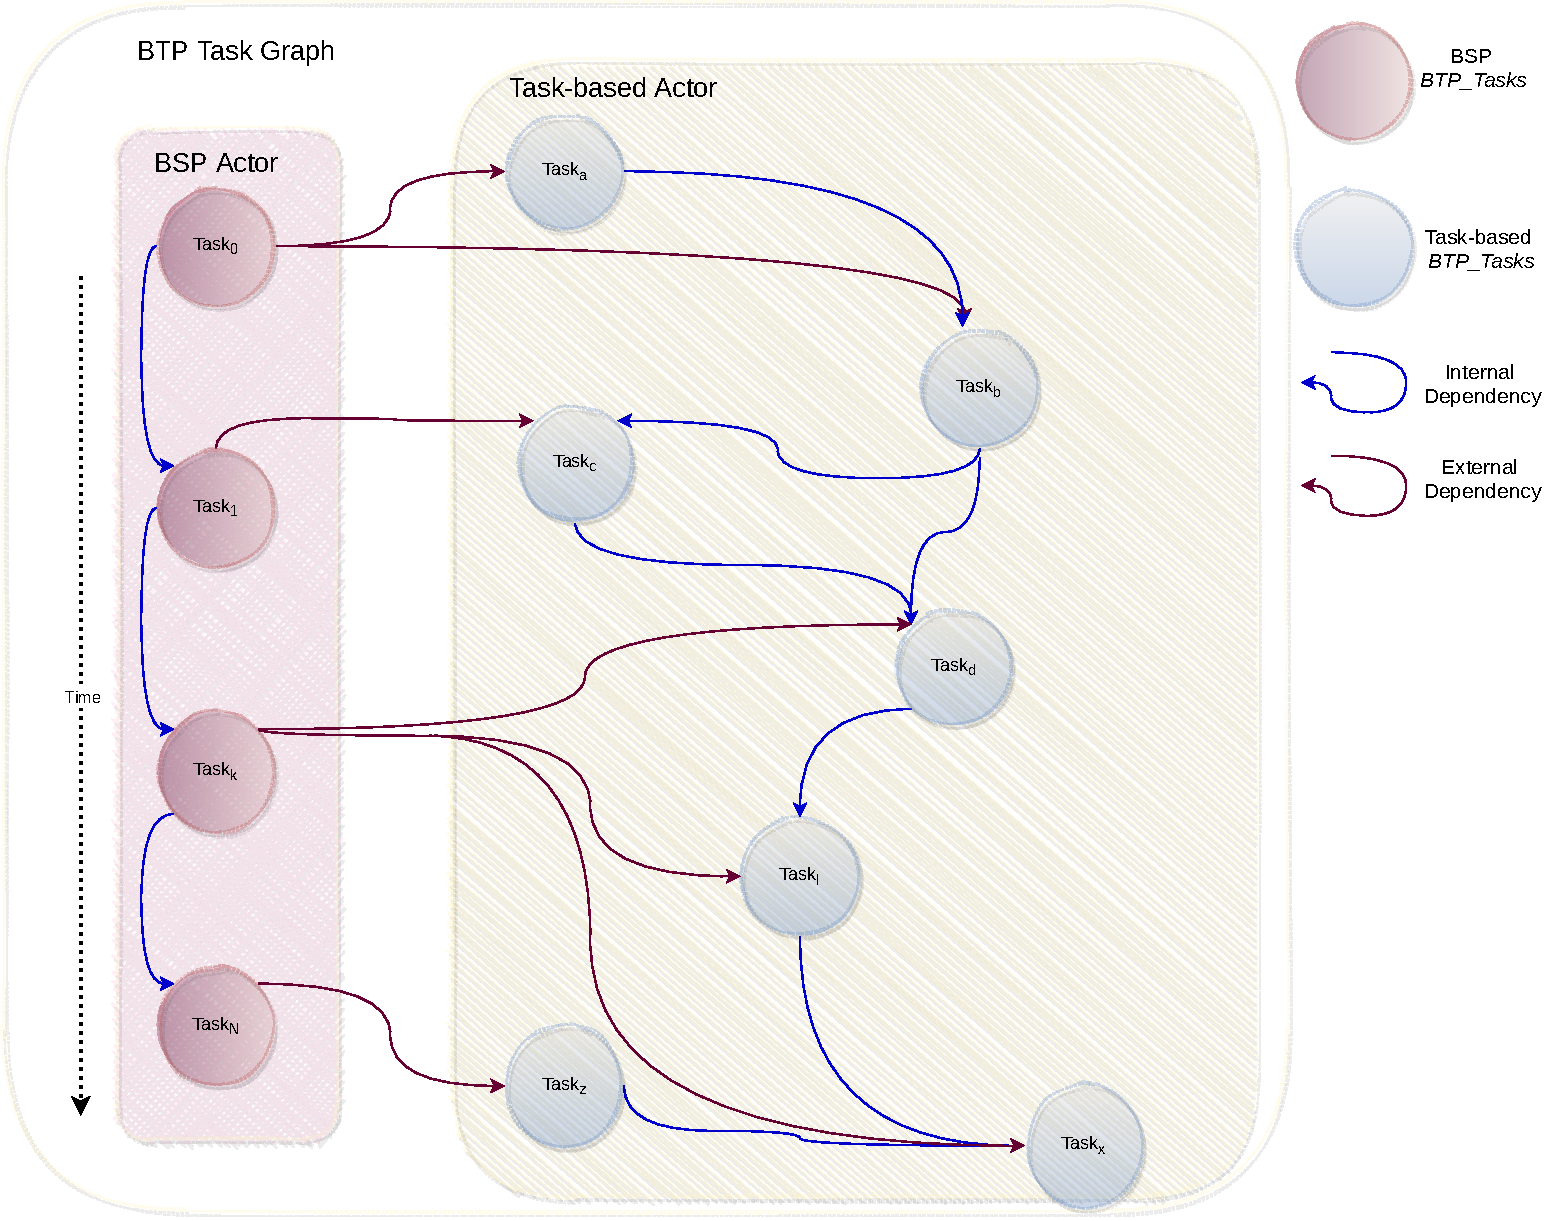
\includegraphics[width=0.75\columnwidth]{figures/BTPTaskGraph.pdf}
\caption{\deisa task graph of two coupled components: an MPI component in the left and a task-based component in the right. Note that all the tasks have either an external output on input.}
\label{figWUG}
\end{figure}

\subsubsection{\deisa Delivery Facility}\label{DF}
In addition to ensuring the establishment of connections between components, the \textit{Delivery Facility} (DF) ensures a global identification and redistribution of data between coupled components. 
It identifies a piece of data internally in a component and translates its identifier to a global ID understandable in other components. This step is essential due to the different ways data is defined in the two paradigms. The DF also implements data redistribution schemes, as the components deal with distributed data structures that are not necessarily distributed in the same way.   

% \ subsection{Exchange Point}\label{EP}

%An \textit{Exchange Point} (EP) can be defined as an entry point to the BTP bridging model; an component shares its internal data with other components through it. The main motivation to introduce \textit{Exchange points} is to keep a good separation of concerns. It provides a clean way to couple components. For instance, component $A$ can, through its \textit{EPs}, expose an array \textit{A} for external use. component $B$ does not need to know how component $A$ computes this array, and component $A$ does not need to know how component $B$ will use it.

%The only way to get information about data an component generates is by establishing a connection with it through a \textit{Delivery Facility} and checking available data (the data that $A$ wants to share) in the \textit{Exchange points}.


\subsection{Assumptions}
Now that we have defined the main concepts and terminology, we define the main requirements and assumptions for a working bridging model in this section. 

We recall that partial ordering is a binary relation $\Re$, defined on a set of events X, which is:
\begin{itemize}
    \item reflexive: $x\Re x, $  $\forall x \in X$, 
    \item transitive: $x\Re y $ $\wedge$ $ y \Re z \Rightarrow  x \Re z, $  $\forall x, y, z \in X$,
    \item antisymmetric: If $x\Re y$ $\wedge$ $ y \Re x \Rightarrow  x = y, $  $\forall  x, y \in X$.
\end{itemize}

If $x\Re y $,  we say that $x$ happens before $y$. Thus, we define a temporal error as a violation intended partial ordering of events. 

Here are the main assumptions:
\begin{enumerate}
    \item We consider coupling two components in a producer/consumer scheme.\label{rule1}
    
    \item The producer is a BSP-like program where the partial order of the internal events is respected.\label{rule2}
    
    \item The consumer is a distributed task-based program (framework runtime is included in the component). The partial order of all internal events is respected.\label{rule3}
    
    \item $\forall x \in P$,  $ \forall y \in T $ $ | $ $x \Re y $ $\Rightarrow$ $ x $ $ triggers $ $ y$, where $P$ is the set of external events in the producer, and $T$ is the set of the \deisa tasks in the consumer, $x \in P $ and $y \in T$.\label{rule4}
    
    \item $\forall y \in T', $ $ \exists x \in P' $ $|$ $ x \Re y$, where $T' \subset T$ and $P' \subset P$. $T'$  is the set of \deisa tasks receiving data or control from the producer, and  $P'$ is the set of external events sending data or control to the consumer.\label{rule5}
    
    \item The previous rule is also applicable in the other sense for control messages that the consumer may send to the producer: $\forall x \in P', $ $ \exists y \in T' $ $|$ $ y \Re x$,  where $T' \subset T$ and $P' \subset P$. $T'$  is the set of external events sending control to the consumer, and  $P'$ is the set of \deisa tasks receiving control from the producer.\label{rule6}  

    \item  $\forall x_1, x_2 \in P' $, $ \forall y_1, y_2 \in T' $ $ | $  $x_1 \Re y_1$ $ \wedge $ $x_2 \Re y_2 $  $ \wedge $  $ x_1 < x_2 $ $\notimplies$ $y_1 < y_2$, where $P' \subset P$, $T' \subset T$ and the binary relation $x_1 < x_2$ means that $x_1$ and $x_2$ are partially ordered ($x_1$ happens before $x_2$). $P'$ is the set of external events in the producer that send data to the consumer, and $T'$ are set of \deisa tasks (triggered by an external event).\label{rule7}

    \item The delivery facilities of coupled components must agree on the use of the same identification protocol; the data expected by the consumer must be sent with enough metadata to be well identified and used.\label{rule8}   
    
\end{enumerate}

Assumptions we have made here are important to use this bridging model to couple two components. They ensure a good operation of the coupling. In assumption~\ref{rule1}, \ref{rule2}, \ref{rule3}, we define our scheme and ensure that the separate components are already working and do not have a temporal error. In assumption~\ref{rule4}, we define a relation between external events of two coupled components and make sure that an external event emitted by one of the coupled components triggers an action in the second component. 

Assumption~\ref{rule5} makes sure that consumer components will not be blocked waiting for data or control that will not be sent by the producer. In other words, all reception events in the consumer must have a sending event coming from the producer. 

In assumption~\ref{rule6}, we make sure that control messages that are waited by the producer must have a sending event coming from the consumer, else the producer will be blocked forever waiting for it.  We only talk about control in assumption~\ref{rule6} because we suppose that the producer will not receive data from the consumer. In reactive workflows, we may also include data in this assumption. 

Assumption~\ref{rule7} concerns partial ordering of \deisa tasks in the consumer. Since we assume that the consumer is a task-based component, we do not know when the runtime will launch the tasks, so we can't assume that if the trigger events are partially ordered, the triggered tasks will also be. Since we only add external dependencies to the original task graph, we may only delay the execution of tasks but not falsify the results.     
Assumption~\ref{rule8} makes sure that the data expected by the consumer is sufficiently accompanied by metadata to be integrated as the right external input in the task graph.

\subsection{Full Producer/Consumer Example}\label{sec:btp:FullPCExample}
 
\begin{figure}[tb]\centering
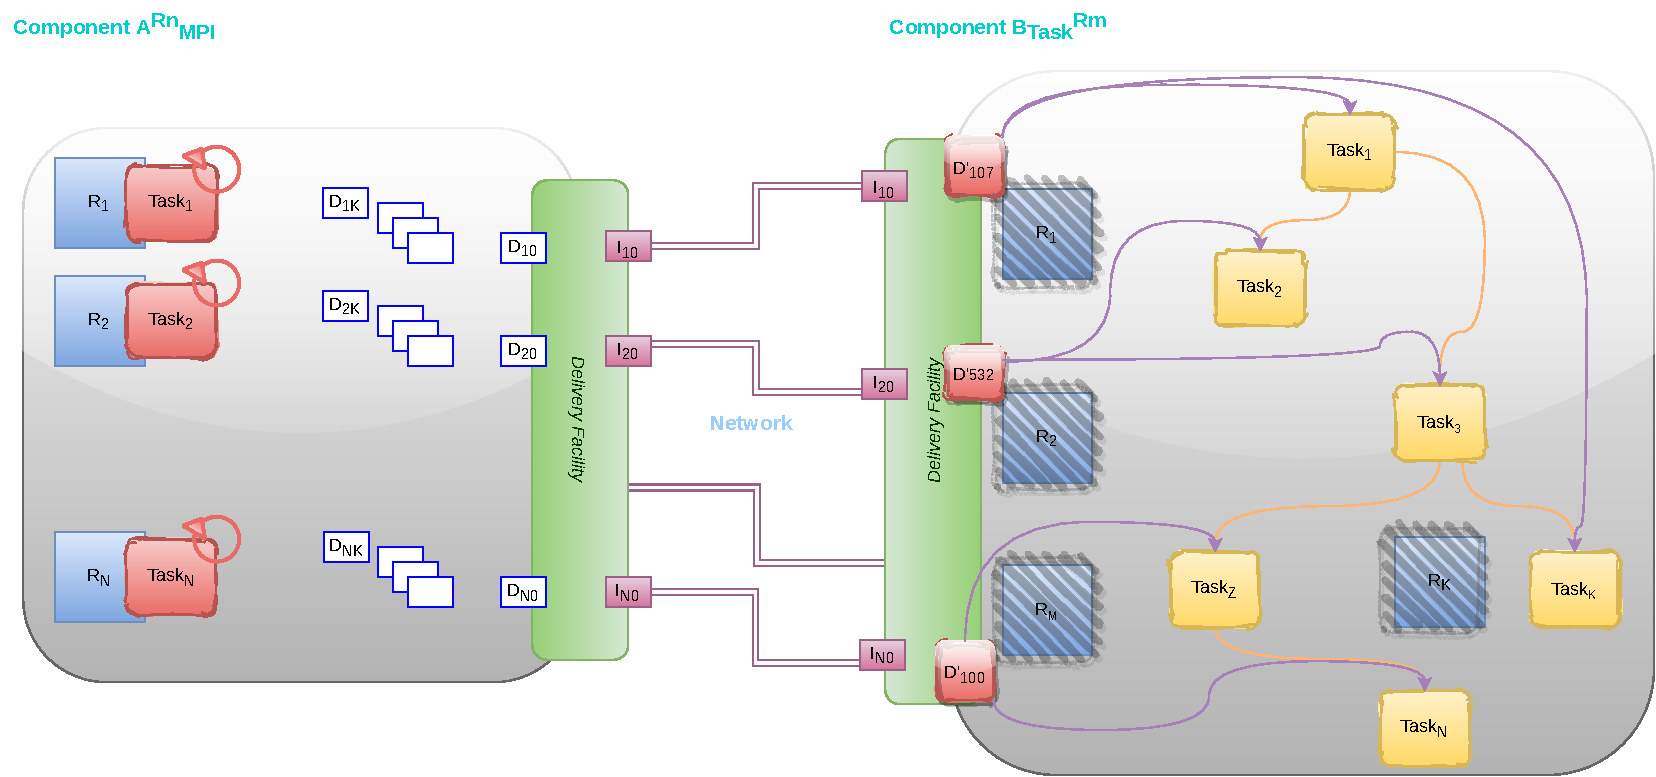
\includegraphics[width=\columnwidth]{figures/BTP.pdf}
\caption{Producer Consumer Example}
\label{figBTP}
\end{figure}

We only show data communication between two \deisa components in this example to simplify the workflow.
Figure~\ref{figBTP} shows an example coupling $A_{MPI}^{R_{n}}$ and $B_{Dask}^{R_{m}}$ where $A$ is a producer and $B$ is a consumer. The MPI component has $R_{n}$ resources. Each $Task_k$ is scheduled explicitly to a set of resources $R_{k}$. In scientific applications, we usually have an iterative code. Each task generates a block of data at a given moment $t$ (only one task is shown in the figure, with a loop mark). Those blocks of the data (small blue boxes $D_{i,j}$) are shared and sent to the \textit{Delivery Facility}.
Component $B$ is the consumer of the data. It is a task-based component that has $R_{m}$ resources that are managed implicitly by a runtime (blue boxes with grey hachures). A task graph is represented as a \deisa task graph (yellow graph), with dependencies on external inputs. Those inputs (in red) are data with new keys (IDs) that are easily recognizable, thus usable in $B$.  

The data is sent through the network between components. The \textit{DFs} ensure the connection to a distant component, identifying and redistributing data between components. 
In this figure, the data identification is made in two steps from each side. The small blue boxes $D_{i,j}$ are identified by three elements: $D$ is the name of the data, $i$ for instance, the position of this block of data in the global distribution, and the $j$ corresponds to the timestep or the iteration. These keys can be considered as being local to the component $A$. 
The same component has created a new key: $I_{l,m}$. It is a global key recognizable in the \textit{DF} of $B$. In the component $B$, those keys are translated to new keys internally understandable $D'_{k}$. 
This identification and translation process is mandatory but can be done in fewer steps. For example, if $I_{l,m}$ is recognizable by $B$, then there is no need for further translation at reception.


\section{\deisa Bridging Model Implementation}\label{sec:btpimplementation}

Several choices have been made regarding the implementation of the bridging model. We have focused on three main goals: performance and separation of concerns on the simulation side and productivity on the analytics side. Those goals have guided all our choices to propose a solution that responds the most to our problematic: bringing together the performance of in situ and the productivity of post hoc workflows.

For that, we have opted for \pdi data interface to handle data and \pdi  plugins to implement the \textit{Delivery facility} engine, \dask distributed as a task-based framework and an \textit{Adaptor} to implement the \textit{Delivery facility} from the analytics component side.
We have chosen MPI for its success and popularity in the HPC community; the huge majority of legacy and new production codes are parallelized in MPI+X. We only focus here on justifying our choice regarding \pdi and \dask distributed.

As already presented in Section~\ref{sec:pdi}, \pdi is a lightweight data handling library that ensures good separation of concerns. It enables sharing of simulation data for external use without any copy, thus its performance. 
%In addition, it has a declarative API and allows changing the data handling approach in the external configuration file without recompiling the simulation code. 
In this work, we have chosen to use \pdi to extract simulation data and implemented the \textit{Data Facility} on top of the pycall plugin in Chapter~\ref{deisachapter} and then through a new \pdi plugin named \deisa in Chapter~\ref{deetitachapter}. In addition to the advantages listed above, \pdi allows switching between different plugins easily, thus switching between in situ and post hoc modes if needed. This is crucial to support heterogeneous workflows to be able to keep analytics results along with raw data in case further analytics are needed. 

In this work, we introduce an ease-of-use in in situ workflows which is comparable to post hoc ones and bring the zen of Python to the HPC community, all in one through \dask distributed framework. 


\subsection{Components}
The BSP component in our work corresponds to a running simulation parallelized with MPI. Since we are interested in HPC simulations, we suppose that they are distributed over multiple processes, thus manipulating distributed data structures.   

The task-based component is a complete \dask distributed cluster running an analytics job. Unlike the simulation, where we only deal with the MPI processes, we deal with three entities in the task-based component: the analytics client, the centralized scheduler and distributed workers that compute the needed job. 

We recall that we only consider a producer/consumer scheme where the producer is the simulation and the consumer is \dask. In this chapter, we will make an abstraction of the concept of \deisa tasks and \deisa task graphs for simplification; we will need it back in Chapter~\ref{deisachapter}. 

\subsection{External Events}

We have respected the information hiding and separation of concerns modularity principles. All internal events are hidden at this point, and the components may share data only through external events. 
In the MPI simulation, we have introduced external events thanks to \pdi data interface that allows sharing of internal data for external use. Once the data is shared via \pdi, it is handled by our dedicated.

In \dask,  an external event is usually input data coming from the simulation and integrated into the task graph. We will detail that in the next section.   



\subsection{MPI Simulation Delivery facility: Bridge}\label{sec:bridge}
The delivery facility in the most important entity, as it ensures the real coupling and communication between the different components.
The delivery facility in the simulation component is called the \textit{Bridge}, 
It is built on a lightweight \dask client that is only used to send data to the workers and communicates metadata with the analytics client. It is implemented as a Python class.

We have implemented a \pdi plugin that creates a bridge in each MPI process. Thus,  the delivery on the MPI side can be seen as a set of distributed lightweight \dask clients. They ensure the connection to the \dask scheduler (so the task-based component). They also ensure the identification (Section \ref{sec:datamodel:dataid}) and communication of the data. 
We have opted to use \texttt{scatter} to send data from the  bridges to the \dask workers. To communicate metadata, we have used \dask \texttt{Queue}s and \texttt{Variable}s. We will detail the different mechanisms in the next sections.  


\subsection{\dask Analytics Delivery facility: Adaptor}\label{sec:adaptor}

The delivery facility in the \dask component is called the \textit{Adapter}. It is associated with the main \dask client. It ensures communication with the \deisa bridges through the scheduler via \texttt{Queue}s and \texttt{Variable}s
Sending the data to the workers is not enough; metadata has to be sent to the adaptor to keep the semantics of the data blocks sent independently and use them in meaningful analysis. 


\subsection{Data and Control Communication}\label{sec:DandCcomm}

To ensure the coupling of MPI with \dask, both data and control need to be exchanged. Several communication schemes can be considered. For instance, in a producer/consumer scheme, data can be pushed by the producer in the consumer's memory, or the consumer can pull the data from the producer. A staging memory can be deployed to host generated data before the consumer retrieves it. This works for the control as well.      
In this work, the delivery facilities ensure the data and control communications. We have opted for a push scheme where the BSP component pushes the generated data to the distributed task-based component when it is ready. 

\subsubsection{Control Communication}\label{sec:DandCcomm:control}
Control in in situ coupling can be defined as events that are exchanged between data producers and consumers to trigger actions. We have used that to coordinate several operations. In this work, all control goes through the \dask scheduler. The scheduler's memory can be seen as a staging area between the two components. We have used available data structures in \dask to communicate control, namely \texttt{Queues} and \texttt{Variables}. 

\paragraph{Control Communication with \dask Distributed Queues} 
The definition of a \texttt{Queue} in \dask is similar to python \texttt{Queue} where data is stored in a First In First Out (FIFO) fashion. The main difference is that in \dask, the \texttt{Queue}s can be accessed by multi-producers and multi-consumers \dask clients. 
We have used the \texttt{Queue}s to communicate metadata that have to be accessed only once and only by one consumer. A typical use is to store the metadata associated with the data generated by an MPI process.  

\paragraph{Control Communication with \dask Variables}
\texttt{Variable}s in \dask are mutable variables that allow sharing of data values between all connected clients. Unlike the \texttt{Queue}s, the data stored in a \dask \texttt{Variable} can be accessed and modified by several clients at the same time. The way they are used in our implementation avoids any possible race conditions that may occur; we have used them only for immutable data, and we have only one writer and several readers.
We have used \texttt{Variable}s to share metadata that have to be accessed by all the bridges. The adaptor is the only writer in the \texttt{Variable}s. For instance, the list of connected workers is stored in one shared \texttt{Variable}.  

\paragraph{Synchronization with \dask Variables}
The \texttt{Variable}s have an interesting property: a reader is blocked while the \texttt{Variable} is not initialized yet. We have used this property to synchronize the simulation and \dask represented by the bridges and the adaptor, respectively.  

For instance, the analytics client waits actively until all workers connect; we assume that the analytics client already knows the number of needed workers. once those workers get connected, it puts a list of all the workers' IP addresses in a variable called \texttt{Workers}, which is accessible to the bridges that are blocked until this variable is initialized. Each bridge gets the same list of workers.

The way we implement the synchronization today is not different from making all bridges wait until all workers are connected and get the list from the scheduler directly. Both solutions imply requesting data from the scheduler, which may be an issue while increasing the number of associated MPI processes. This is because both information comes from the scheduler. Trying to get the list of connected workers or the content of a variable implies requests to the same entity, which is the scheduler. However, the implementation of the bridges may be changed, and communications between those and the adaptor may be improved to bypass the scheduler. And at that moment, our current implementation will make a lot of sense.    

\subsubsection{Data Communication}\label{sec:DandCcomm:data}
Data communication is the most important part of the in situ paradigm. All the solution is built around how data is communicated between the producer and the consumer. 
Data can be kept in shared memory between the two parts, may be copied to another memory or even sent via the network to other nodes. 
We have opted for this last solution and separated the two components' resources. Our solution is in transit. 
We have chosen to push generated data by a simulation process to \dask workers' memory without any staging area and the associated metadata to the analytics client, thanks to the bridges (Section\ref{sec:bridge}) and the adaptor (Section\ref{sec:adaptor}.

\subsection{Control Flow}\label{sec:dataflow}

In a producer/consumer architecture, data flow must be controlled correctly. For instance, if the producer is faster than the consumer, the system still works thanks to data flow management. In this case, there are several ways to manage the flow of data, and the most intuitive one is to block the producer until there is enough memory in the consumer. Other solutions may propose having a staging area to store the data if the producer is full or just writing the data to disk. 
In this work, we have opted for the trivial solution. The simulation is blocked while \dask is still processing data from previous timesteps.  

We have used the \dask distributed \texttt{Queue}s system to manage the data flow thanks to the \texttt{Queue.size} attribute. We can set the size of the \texttt{Queue} depending on the total memory size of the workers and the size of the data generated per timestep. This solution is possible only when it analytics are submitted at each time step. For instance, we can identify whether data from a given timestep is processed, depending on if its associated metadata is pulled from the \texttt{Queue}. 

\subsection{Data Model}\label{sec:btpImp:datamodel}

Data is one of the core concepts of our work; its definition, identification, representation, and communication are as important as its processing. To smooth  differences between BSP and task-based model, the \textit{Delivery Facilities} from both sides, being aware of the semantics of data, add a layer to make it understandable to other components. We will detail in the following sections how we managed the data in \deisa bridging model regardless of all the differences in data semantics and definitions.

\subsubsection{Data Semantics}\label{sec:datasemantic}

In order to couple a BSP component and a task-based one, we have to map data generated by the first to the task graph managed by the second while preserving their semantics. As \deisa components hold distributed data structures and exchange blocks rather than the whole data, the semantics may easily be lost while communicating.  
A possible way to preserve the semantics of the data is by uniquely identifying the blocks generated by the simulation (as defined in section\ref{defdataBSP}) and mapping them as inputs to the task graph as a pure data task (as defined in section\ref{sec:puredata}). 

In this section, we provide a clear definition of the data in each model; this is important because all the following sections are based on those definitions.

\paragraph{Definition:}\label{defdataBSP}
In the BSP model, data can be defined as a \textbf{value} of a buffer at a given timestep. In MPI, the name of this buffer, an MPI communicator, the rank of the process, and the timestep are needed to identify data in the global distribution of the generated array by a simulation over time. 

\paragraph{Definition:}\label{defdatataskbased}
Data in a task-based model can be defined as an \textbf{input} of a or many tasks. Data may be ordinary objects, files, or pure data arrays from external resources. In work, we are mainly interested in simulation-generated data provided as inputs to the task-based component. In \dask,  our solution is built on the pure data tasks (as defined in section\ref{sec:puredata}), which are nothing else than pure data arrays. 


\subsubsection{Data Representation and Identification}

A \deisa component can manage distributed data structures and process them. Distributed data structures are builtin concepts in several tools nowadays; high-level APIs already exist to manage those such as \texttt{dask.array}s, \texttt{dask.dataframs}s in \dask, \texttt{region}s in Pygion, \textit{Ds-array} in PyCOMPSs and others. 
The common characteristic of those data structures is that they are virtual; they may be distributed over several nodes, and the whole data structure may not exist simultaneously in the memory. 
Each array represents a coherent multidimensional field. An array is split into blocks. Each block should be identified in a way that allows a receiver component to know the component it comes from, the field it belongs to and its position in the spatio-temporal decomposition. 

\paragraph{Data Representation}\label{sec:datamodel:datarepresent}

%Deisa virtual arrays in synch or numpy arrays in asynch and dask arrays 
%from the simulation side as a mirror of the dask array that we create in the client side.

One of our motivations for using \dask, was the relevant high-level APIs it offers. The one that corresponds the most to our need is the \texttt{dask.arrays} API. 
A \texttt{dask.arrays} is a virtual representation of a multidimensional array broken down into several blocks called chunks. It can be used, for instance, to read an HDF5 dataset in post hoc case, so it would be appreciated by the user if we keep the same API. 
We have chosen to provide a \texttt{dask.array} per generated data field.  
This representation can preserve decomposition information of out-of-memory problems through chunks definition. 
Note that the user can jump from \texttt{dask.arrays} to \texttt{dask.dataframes} easily and can use lower-level APIs alongside \texttt{dask.array} if needed. For instance, when he wants to use specific methods from \texttt{Pandas} API (\texttt{dask.dataframes}).

While we had a simple choice for the \dask side, we have two equivalent data representations for the simulation:
either keeping a basic representation, where we associate each generated block with a set of metadata, and we push them to \dask; 
or proposing a virtual data structure, similar to \texttt{dask.arrays} to represent the global view of the generated blocks.  
We suppose we have a perfect decomposition of the shared array; all participating processes generate the same shape and size of data. 
For both possibilities, all the changes will be added on the configuration side rather than in the simulation file. So the user will not need to change the way he implements the simulation. 

We have provided both implementations of data representations; technical details are shown in Chapter~\ref{deisachapter}.

\paragraph{Data Definition}\label{sec:datamodel:datadef}
%from ptr - pdi store -  pybind - numpy - dask

When data is shared with \pdi, it only gets a pointer to that data rather than making a copy unless it is defined as metadata in the specification tree (see Section~\ref{sec:pdi} for more details about \pdi). 
The bridge is built on \pdi with python support, and \pdi uses already \texttt{pybind11} to expose C++ types to python. Thus, the bridge uses it too. 
When data is shared with \pdi and has to be handled by the bridge, a pointer of that data is passed to \pdi and transformed into a \texttt{numpy} array by \texttt{pybind11} then passed to the bridge alongside other the metadata allowing the identification of this array.
Note that there is no copy that is performed, and all those steps are done in the master thread of the MPI process sharing its data. 

In \dask side, we define our data as \texttt{dask.arrays}. We use the metadata we get in the adaptor to reconstruct the global view of the domain decomposition. Each block in \texttt{dask.array} corresponds to a \texttt{numpy} array generated per an MPI process in the simulation and sent to \dask. 

\paragraph{Data Identification}\label{sec:datamodel:dataid}
%metadata
%what and how and why 
%keys we get from a scatter, the size and position are sent 
%used for dask array creation 

To smooth the differences in the data semantics, we uniquely identify each value of a given buffer produced in the BSP model. This step consists of associating a unique \textit{key} to a buffer's value at a given timestep and using this same \textit{keys} in the creation of the corresponding \texttt{dask.arrays} in \dask side. We have two main possibilities here: to use \dask key-management system or to develop our key-manager. 
Both solutions have pros and cons, and opting for one or the other changes the design of our coupling system. Using the \dask key-management system gives rise to a synchronous implementation of \deisa, and the second gives rise to an asynchronous one. 

\paragraph*{\dask Key Management}\label{sec:synchimplementation}

This solution is based on \dask \textit{key} management system in addition to a set of metadata (data name and its position in the global decomposition). Once data is generated by an MPI process, the set of metadata is associated with it.  We have used \texttt{scatter} method to send data generated by the simulation to the \dask workers.
The \texttt{Future} returned by the \texttt{scatter} function is appended to the metadata and sent to the scheduler. The \textit{key} returned by the \texttt{scatter} is unique. Thus the data can be identified in \dask by that unique \textit{key}. 

\dask has to wait for the returned \texttt{Future} by the \texttt{scatter} to be able to use the data for analytics, thus, the synchronicity of this solution. 

\paragraph*{Asynchronous Key Management}\label{sec:asynchimplementation}

In the previous version, the keys associated with the data generated by the simulation were managed by \dask. To provide an asynchronous solution, we have provided a common key-manager that is used in both components' data facilities. Thus, it is possible to know all the keys of the data that the BSP component will generate in advance. 
Having this information allows us to create the associated \texttt{dask.arrays} and submit tasks on them in advance (before they are generated), thus the asynchronicity of this solution.

We have introduced a new concept in \dask to implement this solution: namely external tasks. We will provide more details on that in the next sections. 
 


\subsection{Porting an MPI code to \deisa semantics}\label{sec:btp:porting}

\begin{figure*}[tb]
\centerline{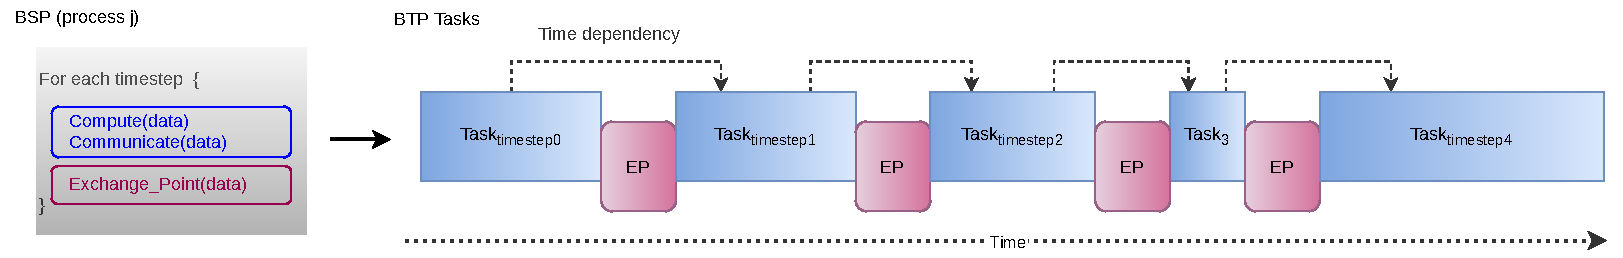
\includegraphics[width=\textwidth]{figures/unrolled.pdf}}
\caption{Example of \deisa representation for an iterative MPI code}
\label{figunroll}
\end{figure*}

The MPI code does not need to be rewritten to be designed in the \deisa semantic. What needs to be done is only to tag the data we want to share externally and specify when this will be done. Concretely, calls to external events are added in the simulation code to make data available for external use. A \deisa task, in MPI words, is a set of computations and internal communications delimited by two external events; concretely, it is all the code that is delimited by two calls of \texttt{pdi\_expose}. The call to \texttt{pdi\_expose} that is added at the end of each iteration in the loop in fig.~\ref{figunroll} is enough to construct a list of \textit{\deisa tasks}, one per each time step. It can be seen as an unrolled loop over time.



%%%%%%%%%%%%%%%%%%%%%%%%%%%%%%%%%%%%%%%%%%%%%%%%%%%%%%%%%%%%%%
%%%%%%%%%% DEISA %%%%%%%%%%%%%%%%%%%%%%%%%%%%%%%%%%%%%%%%%%%%%
%%%%%%%%%%%%%%%%%%%%%%%%%%%%%%%%%%%%%%%%%%%%%%%%%%%%%%%%%%%%%%

\chapter{Deisa: \dask-Enabled In Situ Analytics} \label{deisachapter}
\vspace{20mm}

\epigraph{\textit{Everything is theoretically impossible until it is done}} {Robert A. Heinlein}
\vfill


In \deisa~\cite{deisa}, we have implemented the synchronous version of the bridging model called \deisa. \deisa: \dask-Enabled In Situ Analytics, or more precisely in transit, because we launch each component on separate nodes. In \deisa, we have used the \dask key management system, the available \texttt{scatter} method to send data to \dask workers and a task graph is submitted at each time step. 
In this section, we will detail the architecture of \deisa, its implementation, its operation, and its limitations.  

\newpage

\section{Architecture}
Figure~\ref{figdeida} shows the architecture of the \deisa prototype. We couple a running simulation represented by $M+1$ MPI processes with a \dask instance which includes a scheduler, an analytics client and $N$ workers.
Simulation data is handled with the \pdi data interface. It is shared at each timestep (or periodically every $K$ timesteps) through the \texttt{pdi\_expose} function with the \deisa plugin that instantiates a bridge object per MPI process. 

Each bridge connects a \dask client to the scheduler. The bridge clients only send the data to the workers and a set of metadata to the scheduler and do not submit any task graph to the scheduler. 
At each timestep, the generated data by each MPI process is sent to a pre-selected \dask worker (step $1$ in Figure~\ref{figdeida}). Each bridge constructs a set of metadata regarding the generated block in the attached process that includes the name of the data, its type and subtype, its size and the timestep. That metadata is sent to the scheduler in a \dask \texttt{Queue} associated with the bridge (step $2$ in Figure~\ref{figdeida}). 

The delivery facility in the \dask side is called a \deisa \textit{Adaptor} or also called metadata adaptor. At each timestep, it requests the metadata from the scheduler (which is/will be available in the queues); uses them to create a \texttt{dask.array}. It creates one \textit{dask.array} per block of data received from an MPI process. Then it gathers all the blocks in one larger array using the available \texttt{dask.array.block} method (step $3$ in Figure~\ref{figdeida}). 

The client retrieves this \texttt{dask.array}, which is only a descriptor of the actual data that resides in the workers' distributed memory and submits a task graph on it (step $4$ in Figure~\ref{figdeida}). 

This process is done at each timestep, only after the communication of the data to \dask workers, thus its synchronicity. 


\begin{figure}\centering
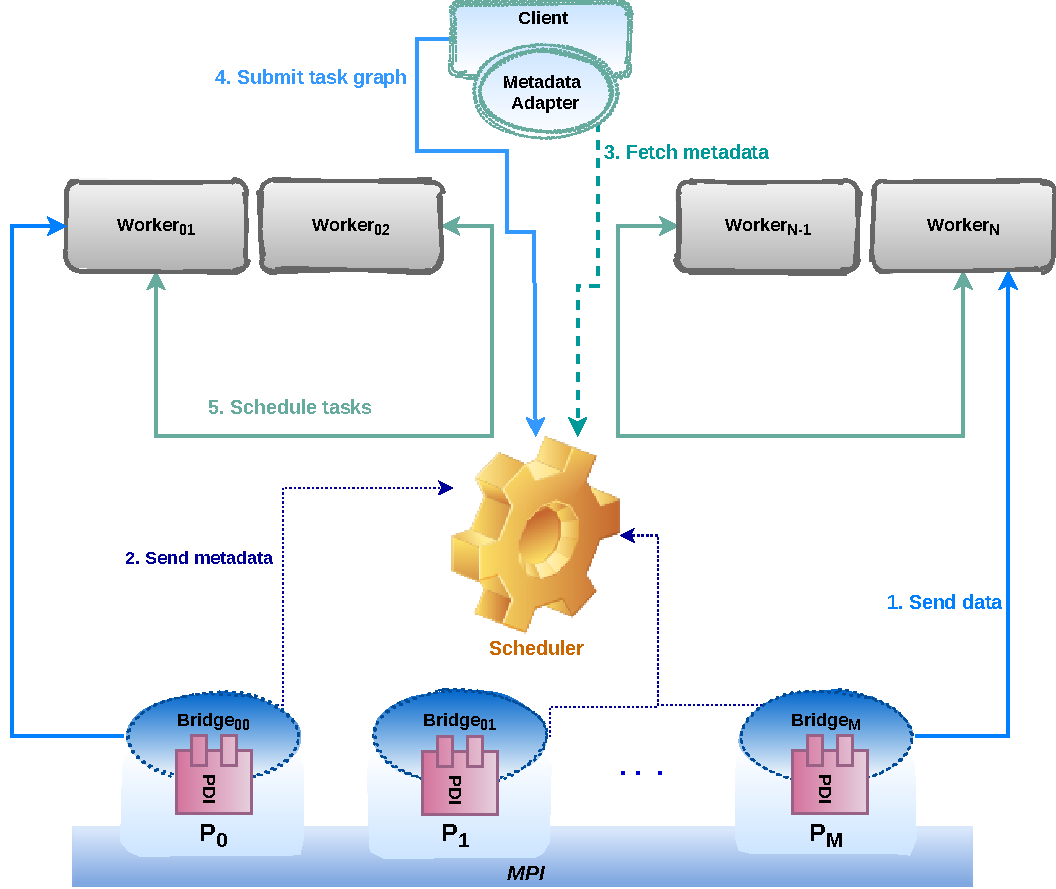
\includegraphics[width=\columnwidth]{figures/DeisaV1.pdf}
\caption{\deisa architecture}
\label{figdeida}
\end{figure}


\section{Implementation}
As already mentioned in the previous section, we have tried to use as much as possible the available functionalities in \dask. A deep understanding of \dask was required to ensure the coupled distributed systems' operation. We will detail in the next sections the operation of the coupling of the two distributed applications.

\subsection{Data and metadata Communication}\label{sec:datametadacomm}
%bypass GC, scatter  ..
%create dask array from future delayed 

When data is available in an MPI process, it is shared with \pdi via \texttt{pdi\_expose}. The pointer of that data is transformed into a \texttt{numpy} array by \texttt{pybind11}, and passed to the \deisa plugin that implements the delivery facility from the simulation side. 
The array is sent to a pre-selected \dask worker via an available method called \texttt{scatter}. 
The \texttt{scatter} is a method in the \dask \texttt{Client} class. It is meant to send pieces of data from the client to the workers directly or by passing through the scheduler. Here are the most important arguments of the \texttt{scatter} method: 
\texttt{scatter(data, workers=None, broadcast=False, direct=None,...)}. Iit returns a \texttt{Future} object (or a structure of \textit{Future}s matching the input data type) pointing to the data that has been sent to the workers. 
In our case, the data is the received \texttt{numpy} array available in the bridge. We enable \textit{direct} mode to send data directly to the workers without passing by the scheduler, to avoid slowing down the scheduler and make it possible to communicate data larger to memory between the coupled components. We specify the IP address of the worker destination. We get in return a \texttt{Future} object, including a unique key generated by \dask.

In this prototype, we did not change the implementation of the \texttt{scatter}, thus, we will consider it a block box that ensures the communication of the data. In Section~\ref{sec:datacommscatter}, we will detail the scatter's internal operation. 

The metadata associated with each generated block is gathered in a python dictionary that includes:  the name of the data, its size and type, and its position in the global distribution as a tuple (including the time dimension in position: 0).  A dictionary is \texttt{msgpack} codable; thus it can be sent via a \texttt{Queue} to the \deisa adaptor in the analytics client of \dask. However, these metadata are not enough to identify data in \dask. The associated key (generated by \dask) with each block of data is required, so it has to be included in the metadata too. The \texttt{Future} returned by the \texttt{scatter} is also needed to identify the data.

The are three main possibilities to include the \textit{Future} in the metadata: 
\begin{itemize}
    \item Include the \textit{Future} in the same \texttt{Queue} as the other metadata, which is not possible because the \textit{Future}s and the dictionaries are not serializable in the same way. So this solution is not possible with the available serialisers in \dask. 
    
    \item Extract the key of the \textit{Future} and append it to the metadata \texttt{Queue}. The key is enough to identify the data that has been sent to \dask. However, if we only send the key, which is a string, the scheduler will not know that the string included in the \textit{Queue} refers to real data. And if, at that time, the bridge goes out of the scoop, and the analytics client did not create a \textit{Future} with the same key yet, then the scheduler may delete that data because it assumes that no client wants it. So this solution does not work.
    
    \item Use a different \texttt{Queue} to send the \textit{Future} or send it as a separate object in the same \texttt{Queue}. This is the most costly solution in terms of communications. However, it ensures a rigorous operation of our coupling system, as sending the \textit{Future} object via a \texttt{Queue} prevents the scheduler from deleting associated data with that \textit{Future}. 
\end{itemize}

We have chosen to use one \texttt{Queue} per MPI process and send the metadata in 2 steps. First construct the metadata dictionary and put it in a \texttt{Queue}, and when the \texttt{scatter} returns a \textit{Future}, we put it in the same \texttt{Queue}. 
Using one \texttt{Queue} per process instead of a unique \texttt{Queue} for all the processes avoids any confusion with  the metadata sent in two steps that may happen because we don't have any control on the arrival of messages to the \texttt{Queue}. 
We have implemented the \deisa adaptor in the \dask side to be able to deal with that 2-step metadata communication.


\subsection{Metadata Reception and \dask \texttt{array} Creation} 
%We have opted to use the available \dask \texttt{Queue} to send metadata from the bridges to the adaptor. But since there is no control over the arrival order of the messages in the \texttt{Queue} and we want to use them to control the flow (Section~\ref{sec:controlflow}), we have opted to use one \texttt{Queue} per bridge. The bridges will send first the metadata dictionary, and then the \textit{Future} returned by the \texttt{scatter} when it send the associated data.   

At the reception of the metadata in the \deisa adaptor, a \texttt{dask.array} is created with the same \textit{key} as the \textit{Future} and is put in a list of lists in the position it is supposed to be in (that we get from the metadata in the dictionary). Once done, we create a global \texttt{dask.array} using the \texttt{block} method that receives a list of lists of \texttt{dask.arrays} and creates a global array with as many blocks as there is the lists are each dimension.  

Creating a \texttt{dask.array} this way is not the most natural way to go in \dask. Usually, the user gives \dask the sizes of the array in each dimension and the way he wants to chunk it, and \dask creates the corresponding \texttt{dask.array}. 
In our work, we do the other way around where we create first the chunks with the keys that we want (keys we have gotten already from the \texttt{scatter}, to be able to identify the blocks), then we position them correctly in the array as real chunks then create it.
The array creation is transparent to the user.  

\subsection{Control Flow}\label{sec:controlflow}

To manage the data flow in \deisa we have opted to explore the already used \texttt{Queue}s to stop the simulation from pushing data into the \dask workers. As already explained in Section~\ref{sec:datametadacomm}, we have used a \texttt{Queue} per bridge, where we put first the metadata and then the \textit{Future} returned by the \texttt{scatter}. We have used the \texttt{Queue} sizes to control the flow. When a \texttt{Queue} is full, data communication cannot be done.

The minimum size of a \textit{Queue} is two because at each timestep we need to send $2$ messages, and the maximum is $2N$ where N is the maximum of timesteps data the workers can host at the same time. 

When a \texttt{Queue} is full, the bridges are blocked trying to add the next message containing the metadata dictionary in the queue. When they are unblocked, they can finally run the \texttt{scatter} and send the data. 

\begin{figure}\centering
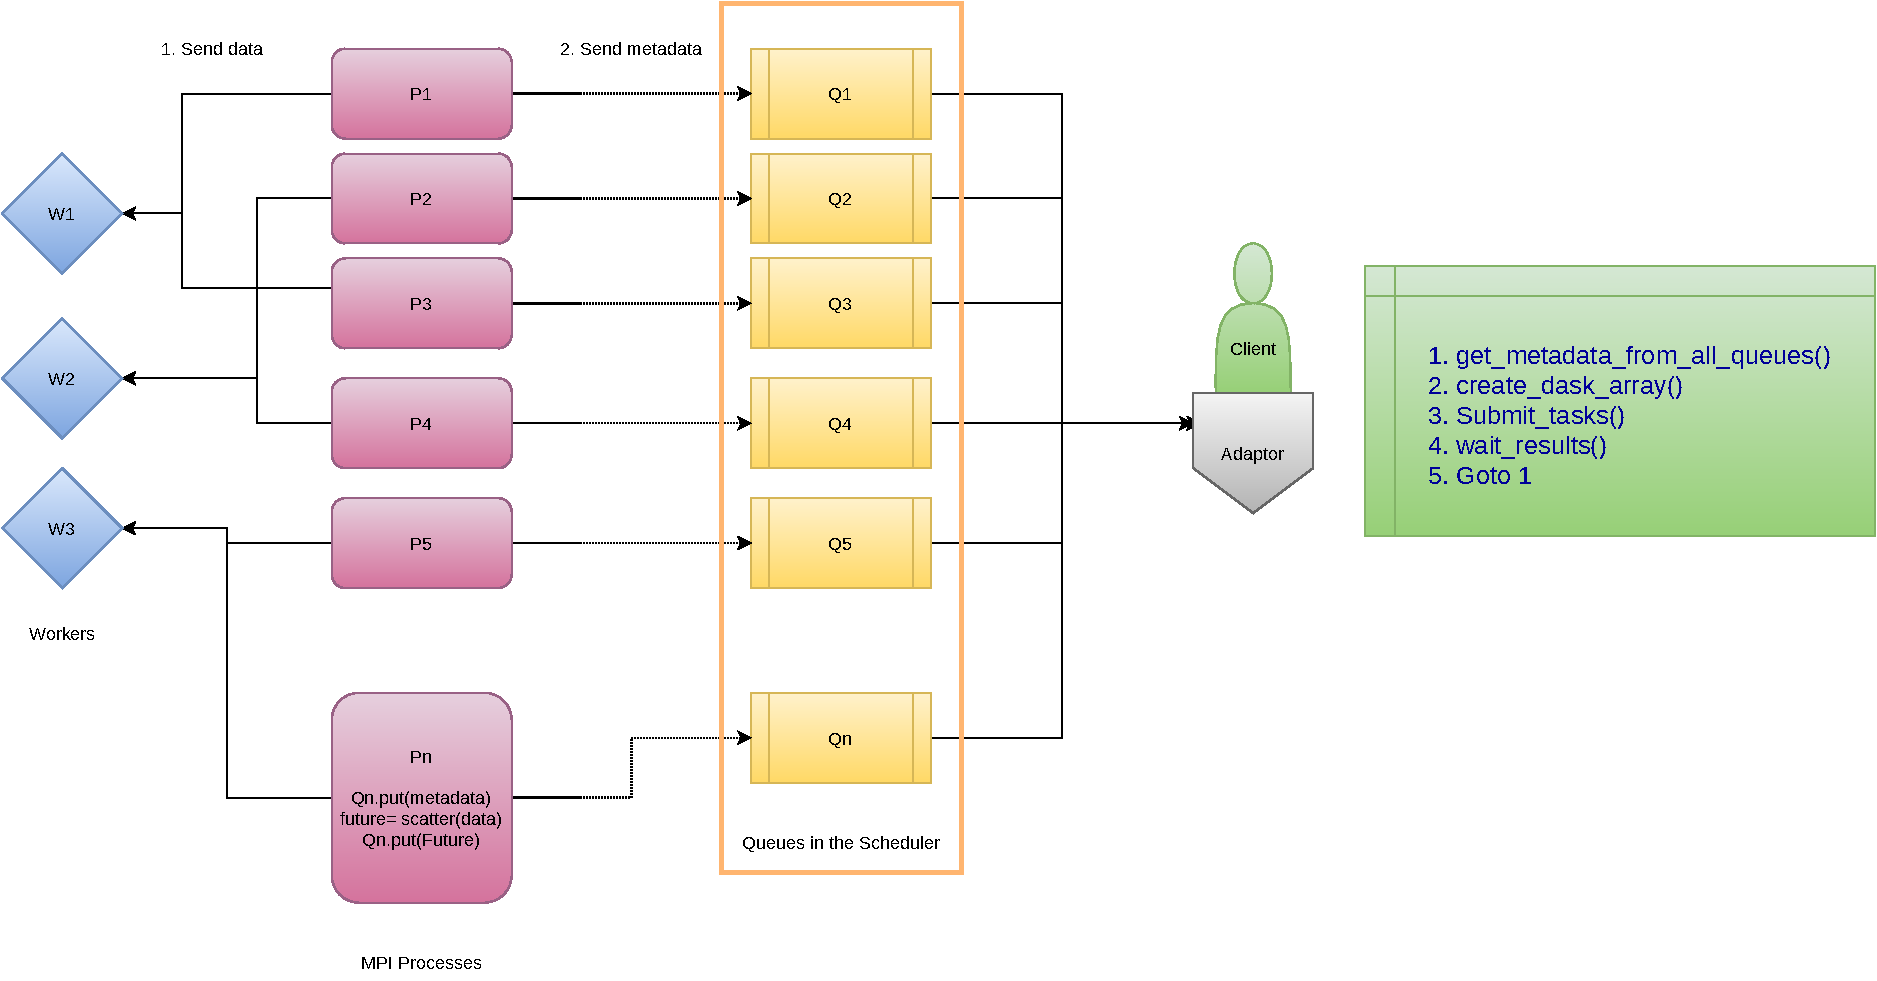
\includegraphics[width=\columnwidth]{figures/controlflow.pdf}
\caption{Control flow}
\label{figdataflow}
\end{figure}

Figure~\ref{figdataflow} shows how the data flow is implemented in the \deisa architecture. We have associated one \texttt{Queue} with each bridge. It will put its metadata into it until it is full: first, the metadata dictionary, then it performs the \textit{scatter} and finally sends the \texttt{Future}. Note that if the bridge is blocked in the first step, the \texttt{scatter} is not done until it is unblocked (the adaptor gets data from the \texttt{Queue}).

The client gets two messages at once from each queue. It constructs the associated arrays with each chunk, then creates the corresponding global array per time step and submits the tasks depending on this \texttt{dask.array}. It can wait or not until the results are computed and then gets the next metadata. 


\subsection{Data Redistribution}
In in transit context, we usually have to deal with a data redistribution scheme. Data blocks are sent from the simulations to the workers. 
The generated blocks by the MPI processes are sent directly to the workers' memory following a round-robin. Each process obtains the list of connected workers and computes the position of the corresponding worker in the list. The position of the corresponding worker is computed using this formula : $worker=list_workers[rank\%len(list_workers)]$.
We suppose that the list of the connected workers will not change during runtime, so at the beginning, the adaptor gets the list of connected workers and puts it in a \dask \texttt{Variable} to be available for the bridges. 
At the reception, the user may want to rechunk data, and this is completely feasible thank to \dask API.

We assume that the user puts enough workers and enough memory in each worker to avoid memory overflows. There is no rule for that, as it depends on the simulation, its duration, the size of the data it generates and the time needed to process that data. 


\subsection{User API and Configuration}
In this section, we present the \deisa plugin configuration and the user API in \deisa. 

\subsubsection{\deisa Bridge User API}
There are three main Methods in the \deisa bridge object, and an initialization function: 

\begin{table}[ht]
\begin{tabular}{||  m{6cm}  m{9cm} ||} 
 \hline
Methods & Documentation\\ 
 \hline\hline
 \texttt{Init(Nbr\_bridges, rank, position, queue\_size) } & Init is a wrapper to initialize the Bridge object.\\ 
 \hline \hline 
\texttt{ Bridge.\_\_init\_\_(Nbr\_bridges, rank, position, queue\_size)} & A bridge object is created, and it initialize the number of bridges, the rank of the MPI process associated with this bridge, the position of the data in the global distribution, and the size of the metadata queue to control the flow. \\ 
 \hline\hline
 \texttt{Bridge.publish\_data(timestep, data)} & This method takes the timestep and the data as parameters, it send the data to the associated worker and the metadata to the corresponding queue. \\
 \hline\hline
 \texttt{Bridge.finalize()} &   This method disconnects the bridge from the scheduler. \\
 \hline
\end{tabular}
\caption{Bridge User API methods}
\label{table:bridge}
\end{table}

In this version of \deisa, we have used the \pdi \texttt{pycall} plugin to call the python API of the bridge. Three main events trigger the bridge methods: \texttt{Init, Available} and \texttt{Finalize}. 
At the initialization step (\texttt{Init} event here), the simulation (Listing~\ref{list:simulation}) shares needed metadata with \pdi to initialize the bridge object. In the \texttt{pycall} specification tree (Listing\ref{list:ymldeisa}), we handle the \texttt{Init} event by calling the \textit{Init} function, offered by Python \deisa API (in Table~\ref{table:bridge}), that initializes the bridge object.

When the simulation sends the \texttt{Available} event along side the data it wants to share for external use, the \texttt{publish\_data()} method handles it in the \texttt{pycall} specification tree. This method sends the data and the metadata to \dask. This part is done inside the main loop, so each time the simulation reaches this \texttt{pdi\_multi\_expose} function, the available data it sent to \dask.  

Finally, when the simulation is finished, we disconnect all the bridges from the \dask scheduler by emitting the \texttt{Finalization} event that it handled by calling the \textit{finalize} method of the bridge. 

All in one, the user has to keep in mind three main steps: at the beginning of the simulation, he has to initialize the coupling by calling \texttt{Init()} that returns a Bridge instance. Every time he wants to share data with \dask, he calls \texttt{Bridge.publish\_data}. And once finished, he disconnects the bridges from \dask by calling \texttt{Bridge.finalize()}.

\begin{lstlisting}[escapeinside={\#}, float, label=list:ymldeisa, language=yaml, caption= Deisa configuration file]
# ...
pdi:
  metadata:
    timestep:     int
    MaxtimeSteps: int 
    pcoord_1d:     int
    pcoord: { type: array, subtype: int, size: 2 }
    dsize:  { type: array, subtype: int, size: 2 }
    psize_1d: int 
    gmax: int 
  data:
    local_t: 
        type: array
        subtype: double
        size: ['$dsize[0]', '$dsize[1]']
  plugins:
    pycall:
      on_event:
        Init: # Initialization step
          with: # Needed parameters
            position: $pcoord
            rank: $pcoord_1d
            mpi_size: $psize_1d
            queue_size: $gmax
          exec: | # Initialize deisa
            from deisa import Init
            Bridge = Init(mpi_size, rank, position, queue_size)
        Available: # Data communication at each `Available` event
          with: 
            timestep: $timestep
            local_t: $local_t
          exec: | # Send data and metadata to the deisa adaptor 
            Bridge.publish_data(timestep, local_t) 
        Finalization: # Finalization step
          with: ~
          exec: | 
            Bridge.finalize()
# ...
\end{lstlisting}


\begin{lstlisting}[float, label=list:simulation, language=c, caption= Simulation main loop]
int main( int argc, char* argv[] )
{
    /*...*/
    // Loop counter referring for the timestep 
    int ii=0;

    // Share useful metadata for initialization step
    PDI_multi_expose( "Init",
                      "pcoord",       pcoord,       PDI_OUT,
                      "pcoord_1d",    &pcoord_1d,   PDI_OUT,
                      "dsize",        dsize,        PDI_OUT,
                      "psize",        psize,        PDI_OUT, 
                      "psize_1d",     &psize_1d,    PDI_OUT,
                      "timestep",     &ii,          PDI_OUT, 
                      "gmax",         &gmax,        PDI_OUT,
                      "MaxtimeSteps", &generations, PDI_OUT,
                      NULL);

    // Main loop
    for (; ii<generations; ++ii) {

        // control simulation duration by performing more substeps
        for (int jj=0; jj<200; ++jj){       
            // Compute the values for the next iteration
            iter(dsize, cur, next);

            // Exchange data with the neighbours
            exchange(cart_comm, next);

            // Swap the current and next values
            double (*tmp)[dsize[1]] = cur; cur = next; next = tmp;
        }

        // Send the `Available` event and share available data with PDI 
        PDI_multi_expose("Available",
                         "timestep",   &ii, PDI_OUT,
                         "local_t",    cur, PDI_OUT,
                         NULL);
        // A barrier to synchronising the processes
        MPI_Barrier(cart_comm);
    }

    // Send the `Finalization event` 
    PDI_multi_event("Finalization"); 

    // Finalize PDI
    PDI_finalize();
/*...*/
}
\end{lstlisting}

\subsubsection{\deisa Adaptor User API}
There are four main functions in the \deisa adaptor user API: 
\begin{table}[ht]  
\begin{tabular}{||  m{6cm}  m{9cm} ||} 
 \hline
Methods & Documentation\\
 \hline\hline
 \texttt{Initialization(Nbr\_bridges, Nbr\_workers) }& Initialization is a wrapper to initialize the Adaptor object.\\ 
 \hline\hline  
\texttt{Adaptor.\_\_init\_\_(Nbr\_bridges, Nbr\_workers)} & An Adaptor object is created; it takes the number of associated bridges and the number of the workers that will be expected. \\ 
 \hline\hline
 \texttt{Adaptor.get\_client()} & This method returns the analytics client created by the Adaptor\\
 \hline\hline
 \texttt{Adaptor.get\_data()} & This method returns the \texttt{dask.array} of a given timestep when available.\\
 \hline\hline
 \texttt{Adaptor.finalization()} &   This method disconnects the clients from the scheduler and shutdown the dask cluster. \\
 \hline
\end{tabular}
\caption{Adaptor User API methods}
\label{table:adaptor}
\end{table}

The user has to initialize the coupling from the \dask side too. In his script, as shown in Listing~\ref{list:deisaanalyse}, he calls the \texttt{Initialization()} function that returns an Adaptor object. The adaptor connects a client to the scheduler, and the \texttt{Adaptor.get\_client()} can be called to get access to it. The metadata sent by the bridges in the queues is retrieved by the client and used to create a \texttt{dask.array}. To get access to it, the user can call \texttt{Adaptor.get\_data()} that returns a \texttt{dask.array} object. This array can be used as any ordinary array in \dask, thus, all the available API\footnote{https://docs.dask.org/en/stable/array-api.html} is usable now.  
To finalize the \dask cluster, the \texttt{Adaptor.finalization()} can be called. This method makes sure that there is no connected bridges and then shuts down the cluster. 

Note that in this synchronous version, one \texttt{dask.array} is created per timestep. Thus if several steps are waited, the \textit{Adaptor.get\_data()} has to be called as many times as needed, and in this version, we suppose that the total number of timesteps is known in advance.

\begin{lstlisting}[float, label=list:daskanalyse, language=python, caption= Dask IPCA code]
import os
import h5py
import dask.array as da
from dask_ml.decomposition import IncrementalPCA

# Connect the analytics client to the scheduler
def connect('scheduler.json'):
    # ...
    return client

client = connect(scheduler_info)

# Dask Configuration 
dask.config.set({"distributed.deploy.lost-worker-timeout": 60, "distributed.workers.memory.spill":0.97, "distributed.workers.memory.target":0.95, "distributed.workers.memory.terminate":0.99 })

# Get HDF5 dataset information
f = h5py.File('data.h5', 'r') 
ds = f['local_t']

# Create a dask array from the dataset with the same chunking as in deisa 
gt = da.from_array(ds, chunks=(1, chunkx, chunky))

# Initialize and compute the incremental PCA
for i in range(len(gt)):
    if i==0:
       ipca=IncrementalPCA(n_components=2,copy=False, svd_solver='randomized') 
    ipca.partial_fit(gt[i])

print("IPCA Algorithm, ", ipca, flush=True)
print("[explained_variance , singular_values]: [", 
      ipca.explained_variance_ , ", ",  ipca.singular_values_], "]", 
      flush=True)

# Clean up    
os.remove('data.h5') 
client.shutdown()

\end{lstlisting}




\begin{lstlisting}[float, label=list:deisaanalyse, language=python, caption= Deisa Client interface]

from deisa import Initialization
import dask.array as da
from dask_ml.decomposition import IncrementalPCA

# Get configuration data
with open(r'config.yml') as file:
    data = yaml.load(file, Loader=yaml.FullLoader)
    Ssize = data["parallelism"]["height"]*data["parallelism"]["width"]
    generations = data["MaxtimeSteps"]
    Sworkers = data["workers"]
    timeStep = 1

# Initialize the Adaptor 
Adaptor = Initialization(Ssize, Sworkers)

# Get a dask client 
Adaptor.client.get_versions(check=True)

# At each timestep we apply a partial_fit
for g in range(0, generations, timeStep):  
    # Get dask array from the Adaptor 
    arrays = Adaptor.get_data()

    # Reshape the data if necessary 
    arrays = da.reshape(arrays, (arrays.shape[1], arrays.shape[2])) 

    # Initialize and compute the Incremental PCA
    if g==0:
        ipca=IncrementalPCA(n_components=2, copy=False, 
                           svd_solver='randomized')

    ipca.partial_fit(arrays)

    # Delete arrays if they are no more needed
    arrays=None

print("IPCA Algorithm, ", ipca, flush=True)
print("[explained_variance , singular_values]: [", 
      ipca.explained_variance_ , ", ",  ipca.singular_values_], "]", 
      flush=True)

# Finalization of dask instance
Adaptor.finalization()
    
\end{lstlisting}

\section{Experiments and Evaluation}\label{sec:evaldeisa}
Now that we have explained how our \deisa prototype operates, we will launch real experiments and evaluate its performance in two supercomputers: Ruche and Irene. This section will detail how \deisa can be used, show the API and configuration, and compare its performance to post hoc analytics.  


\subsection{Launching Experiments}\label{sec:launch}
There are several ways to launch a \dask cluster. However, since our work aims to use \dask for in situ analytics, we have opted to use the command line to include launching both \dask and the simulation in the same submission script and the same job. 
One of the most important motivations for that is the fact that we need both \dask and the simulation launched together for in situ analytics. If we launch them in two different jobs, we do not have control over the starting moment of each. For instance, if data is already available in the simulation, but \dask is in the waiting queue to be started, then we lose the data (if we didn't activate any write). 

To do so, we have used commands already available to launch the different parts of a \dask cluster. Namely, \texttt{dask-scheduler} to start the scheduler process, \texttt{dask-worker} to start worker processes in one or more nodes. The analytics client is launched as a python process also.  

At the end, four steps are launched in one script; the scheduler first creates a file containing the connection information. Once this is done, the client and the workers can be connected, and the simulation is launched.  Launching the steps in the background using \texttt{\&} and Waiting for all the steps is mandatory, else the first finished step will stop the job. 



\subsubsection{Ruche Cluster}\label{sec:ruche}
We have used for our experiments the Ruche\cite{ruche} cluster (Moulon mesocentre, Paris-Saclay). The cluster is composed of 216 ThinkSystem SD530 server nodes; each with 2 Intel Xeon Gold 6230 20C @ 2.1GHz CPUs and 180GB of maximum user-allocatable memory. Each CPU has 20 cores. The interconnect uses Omni-Path 100 Gbit/s and the parallel file system the Spectrum Scale GPFS (IOs rate: 9 GB/s). 
Ruche uses the Slurm job management system.  

Listing~\ref{list:script} shows an example of a submission script in Ruche supercomputer(see Section~\ref{sec:ruche}). This script has four steps, as already described. Each step is launched with \texttt{srun}.
To make sure that the steps are not launched in the same nodes, we use the \texttt{--relative=<n>}\cite{slurm_relative} option of \texttt{srun} that launches the job step relative to node $n$ of the current allocation. In our case, we make sure that each job step is launched in a distinct subset of nodes.  

\begin{lstlisting}[float, label=list:script, language=bash, caption=Submission script of simulation and in situ analytics in Ruche supercomputer]
#!/bin/bash

# Configure the different parameters 
SCHEFILE=scheduler.json
NNODES=$(($SLURM_NNODES-2))
WORKERNODES=$(($NNODES/3))
SIMUNODES=$(($WORKERNODES*2))
NPROC=$(($SIMUNODES*2))                   
NWORKER=$(($WORKERNODES*2))

# Launching the scheduler 
srun -N 1  -n 1 -c 20 --relative 0  dask-scheduler   --protocol tcp  --scheduler-file=$SCHEFILE 1>> scheduler.o  2>> scheduler.e  &

# Wait for the SCHEFILE to be created 
while ! [ -f $SCHEFILE ]; do
    sleep 3
    echo -n .
done


# Connect the client to the Dask scheduler
srun  -N 1 -n 1 -c 20 --relative 0   `which python` -m trace -l -g client.py 1>> client.o 2>> client.e &
client_pid=$!

# Launch Dask workers in the rest of the allocated nodes 
srun  -N $WORKERNODES -n $NWORKER -c 20 --relative 1   dask-worker --local-directory /tmp  --scheduler-file=${SCHEFILE} 1>> worker.o 2>>worker.e  &
     
REL=$(($WORKERNODES+1)
# Launch the simulation code
ccc_mprun  -N $SIMUNODES -n $NPROC -c 20 --relative $REL  ./simulation 1>> simulation.o 2>> simulation.e &

# Wait for the client process to be finished 
wait $client_pid
wait 
       
\end{lstlisting}

\subsubsection{Irene Supercomputer}

We have used the Irene supercomputer in the CEA TGCC centre. We have used the skylake partition. It has 1653 nodes, each with 2 CPUs: CPU: 2x24-cores Intel Skylake@2.7GHz (AVX512), 180GB memory per node. Irene has a total of 79344 cores.  The compute nodes are connected through an EDR InfiniBand network. This high throughput (100Gb/s) and low latency network is used for I/O and communications among nodes of the supercomputer. Irene uses a Luster parallel distributed file system. Script~\ref{list:scriptIrene} show the equivalent submission script in Irene Supercomputer. The main difference is the \texttt{ccc\_mprun} command which is the equivalent of \texttt{srun} in Irene.  

\begin{lstlisting}[float, label=list:scriptIrene, language=bash, caption=Submission script of simulation and in situ analytics in Irene supercomputer]

#!/bin/bash

# Configure the different parameters 
SCHEFILE=scheduler.json
NNODES=$(($SLURM_NNODES-2))
WORKERNODES=$(($NNODES/3))
SIMUNODES=$(($WORKERNODES*2))
NPROC=$(($SIMUNODES*2))                  
NWORKER=$(($WORKERNODES*2))

# prepare the spack environment
ml purge
source $CCCWORKDIR/env_spackuser
unset LD_PRELOAD
unset SELFIE_MPRUN
unset SELFIE_MSUB
export OMP_NUM_THREADS=24

# Launching the scheduler
ccc_mprun -N 1  -n 1 -c 24 -r 0  dask-scheduler --protocol tcp --scheduler-file=$SCHEFILE 1>> scheduler.o  2>> scheduler.e  &

# Wait for the SCHEFILE to be created 
while ! [ -f $SCHEFILE ]; do
    sleep 3
    echo -n .
done


# Connect the client to the Dask scheduler
echo Connect Master Client  
ccc_mprun  -N 1 -n 1 -c 24 -r 1   `which python3` ipca.py 1>> client.o 2>> client.e &
client_pid=$!

# Launch Dask workers in the rest of the allocated nodes 
echo Scheduler booted, Client connected, launching workers 
ccc_mprun  -N $WORKERNODES -n $NWORKER -c 24 -r 2   dask-worker --local-directory /tmp  --scheduler-file=${SCHEFILE} 1>> worker.o 2>>worker.e  &
     
REL=$(($WORKERNODES+2))
# Launch the simulation code
echo Running Simulation 
ccc_mprun  -N $SIMUNODES -n $NPROC -c 24 -r $REL  ./simulation 1>> simulation.o 2>> simulation.e 

# Clean up the files 
`which python3` postscript.py

# Wait for the client process to be finished 
wait $client_pid
wait 
\end{lstlisting}

\subsection{Software}
\subsubsection{Heat2D Mini-App}
We have evaluated our prototype using an implementation of a modified 2D explicit finite difference heat solver. It has been parallelized in MPI using a block domain decomposition, also called a cartesian topology of processes, because the subdomains are squared or rectangular (Listing~\ref{list:simulation}).   
It is representative of a typical 2D Eulerian simulation with stencil computation pattern and MPI ghosts data exchange. Outputs, consisting of the temperature field on the 2D domain, are produced periodically after a fixed number of iterations set to represent a realistic compute-to-output time ratio. 


\subsubsection{Principal Component Analysis}\label{IPCA}
The Principal Component Analysis (PCA), is an important statistical method for dimensionality-reduction. 
Historically in has been invented in 1901 by \textit{Karl Pearson}~\cite{pearson_karl_1901_1430636} and named by \textit{Harold Hotelling}~\cite{10.2307/2333955}.
It is used to reduce the  dimensionality of a dataset, while preserving as much variability (statistical information) as possible\cite{jolliffe2016principal}. 
This is accomplished by linearly transforming the data into a new coordinate system where most of the variation in the data can be described with fewer dimensions than the initial data.

The operation of a PCA can be summarized in those steps \cite{noauthor_principal_nodate, ho_principal_nodate, noauthor_beginners_nodate}: 
\begin{itemize}
    \item Standardization: it aims to standardize the range of the initial variables so that each one of them contributes equally to the decomposition.
    
    \item Covariance Matrix Computation: in this step, the covariance matrix of the initial variables is computed to see all the possible pairs of correlated variables. Note that highly correlated variable contain redundant information.
    
    \item Eigenvectors and Eigenvalues Computation: here, the eigenvectors and the eigenvalues of the covariance matrix are computed to identify the principal components. Geometrically, principal components represent the directions of the data that explain a maximal amount of variance. The covariance matrix's eigenvectors are the axes' directions where there is the most variance (most information), and they are called \textit{Principal Components}. The eigenvalues are simply the coefficients attached to eigenvectors, which give the amount of variance carried in each principal component, and the eigenvectors, in the order of their eigenvalues, highest to lowest, are the principal components in order of significance.
    
    \item Feature Vector: the feature vector is the matrix that has as columns the eigenvectors of the components that we decide to keep

    \item Final Dataset Computation: by recasting the original data along the computed principal components axes. This can be done by multiplying the original dataset's transpose by the feature vector's transpose.
    
\end{itemize}

\texttt{Dask-ML}\footnote{https://ml.dask.org/} library provides scalable machine learning algorithms in Python  using \dask framework and machine learning libraries such as \texttt{Scikit-Learn}\footnote{https://scikit-learn.org/stable/}. \dask-ML provides an implementation of the PCA based on the Singular Value Decomposition (SVD) algorithm\footnote{https://ml.dask.org/modules/generated/dask\_ml.decomposition.PCA.html}.

The PCA needs all the data to be processed in the main memory, which is impossible for large datasets or in situ processing (as data comes as the simulation progresses). The Incremental PCA (IPCA) \footnote{https://ml.dask.org/modules/generated/dask\_ml.decomposition.IncrementalPCA.html} responds to this limitation by processing the data in a minibatch fashion. Furthermore, the IPCA algorithm has a constant memory complexity.    

Listing~\ref{list:deisaanalyse} shows how the IPCA algorithm can be used along side \deisa.

\subsection{Performance Evaluation}

We have performed two main experiments:
\begin{itemize}
    \item \textbf{Experiment I} compares \deisa performance to a baseline with neither IO nor analysis, and to a version using a parallel post hoc analysis with plain \dask.
    \item \textbf{Experiment II} investigates the performance of \deisa more in-depth on large and small data sets to explain its behaviour.
\end{itemize}

\subsubsection{Experiment I}\label{XP1}
Those experiments have been performed in the Irene supercomputer. We have used the developed MiniApp and the Incremental PCA. Table~\ref{parameters1}  and Table~\ref{config1} summarize the used parameters and configurations in these experiments.


\begin{table}[ht]
\centering
\begin{tabular}{||c  c||}
\hline
 Parameter                         & Value \\
\hline\hline
Number of runs                      & 3   \\
Number of iterations IPCA           & 10  \\
 MPI nodes / \dask worker node      & 2   \\
 MPI process / MPI node             & 2   \\
 Dask worker / \dask worker node    & 2   \\
 Thread / \dask worker              & 24  \\
 MPI process / \dask worker         & 2   \\
 \deisa client code                 & Listing~\ref{list:deisaanalyse} \\
 \dask client code                  & Listing~\ref{list:daskanalyse} \\
\hline
\end{tabular}
\caption{\label{parameters1}Fixed parameters used in the Experiment~\ref{XP1}}
\end{table}


\begin{table}[ht]\centering
\begin{tabular}{||cccc||}
\hline
 Configuration              & XP1:128\,MiB  & XP1:256\,MiB  & XP1:512\,MiB   \\
\hline\hline
 MPI block size             & 128                 & 256                  & 512    \\
\dask chunk size            & 128                 & 256                  & 512        \\
\multicolumn{1}{||c}{MPI Nodes}                   &\multicolumn{3}{c||}{[4, 8, 16, 32, 64]} \\
\multicolumn{1}{||c}{\dask Nodes}                 &\multicolumn{3}{c||}{[2, 4, 8, 16, 32] }\\

\hline\hline
\end{tabular}
\caption{\label{config1}The three configurations of Experiment~\ref{XP1}}
\end{table}



\begin{figure}
     \centering
     \begin{subfigure}[b]{0.3\textwidth}
         \centering
         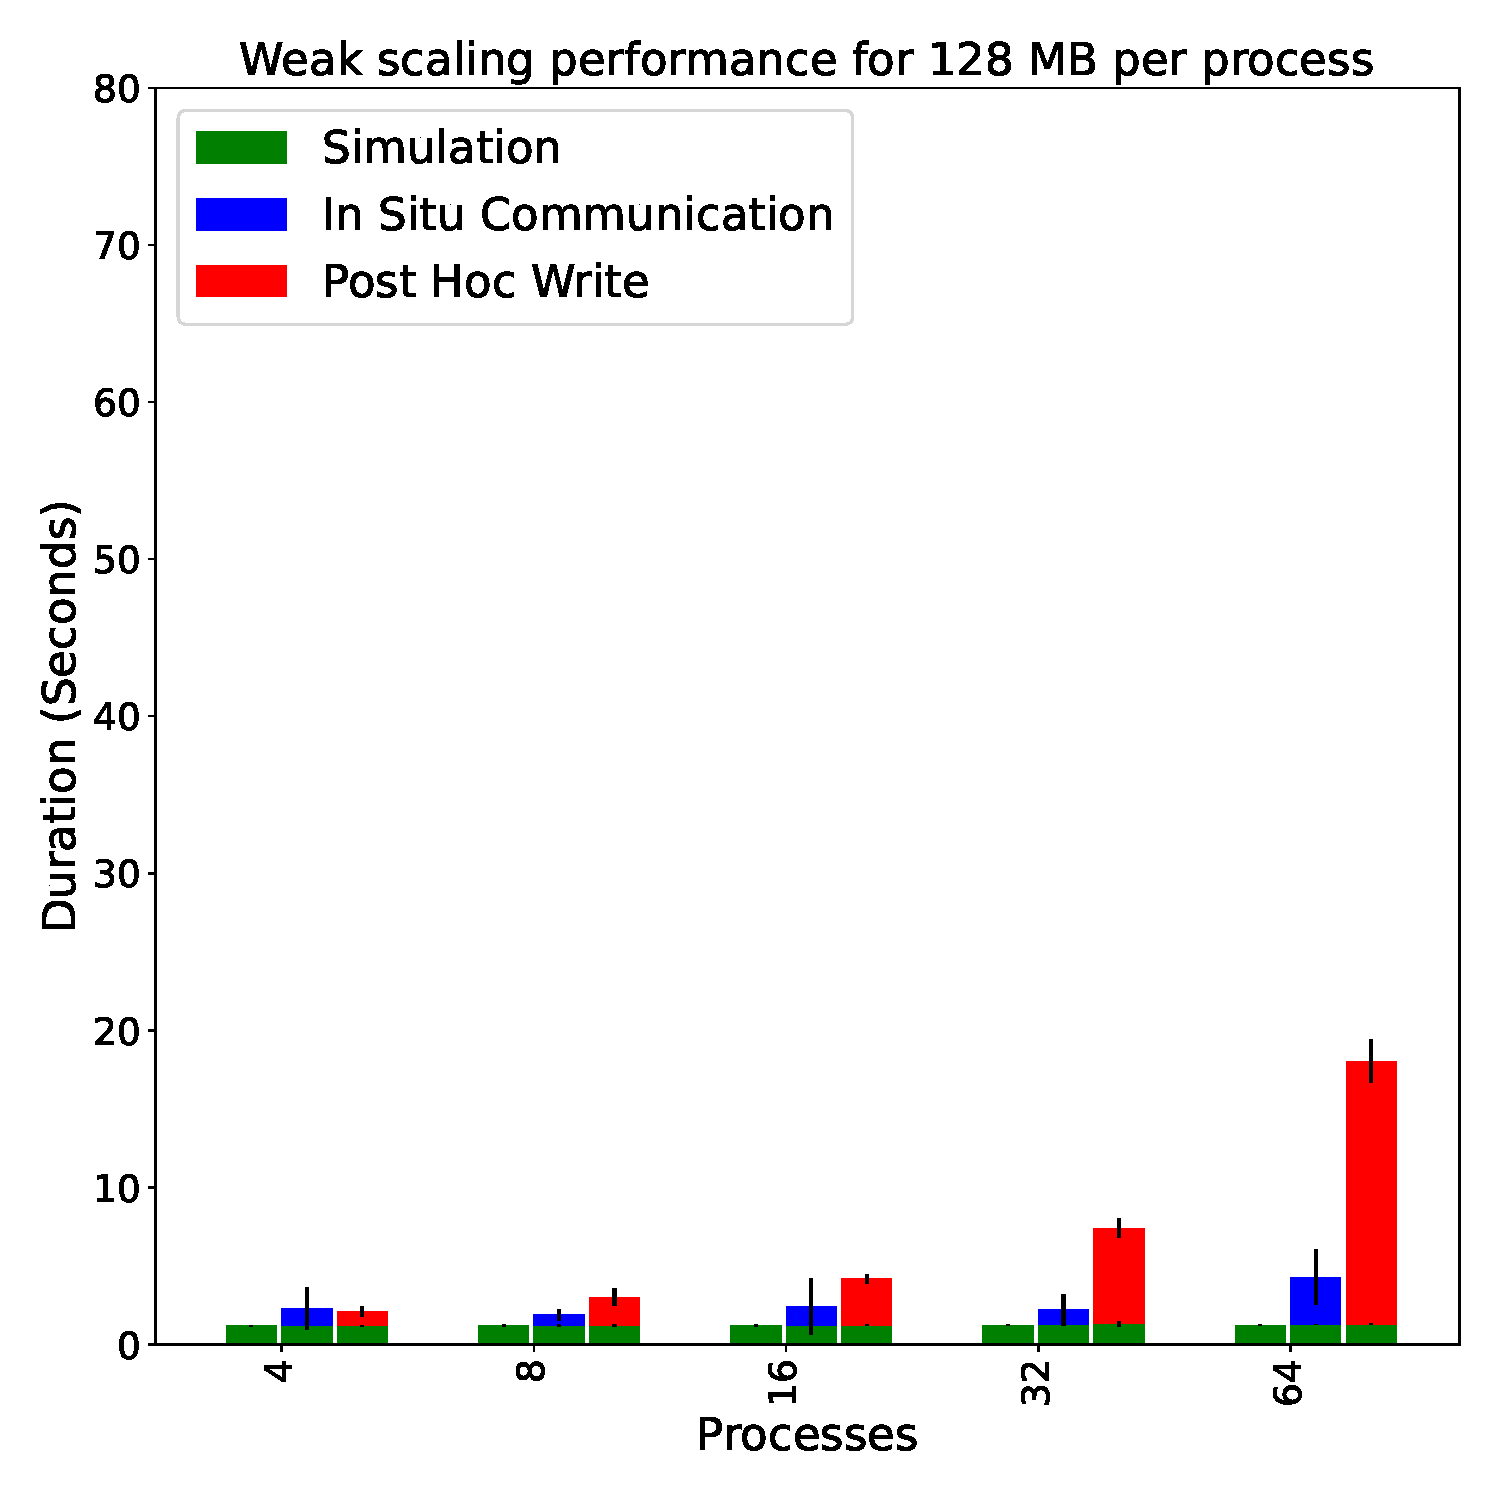
\includegraphics[width=\textwidth, height=\textwidth]{figures/128MB.pdf}
         \caption{Average simulation, communication and IO times per iteration for case: 128\,MiB per process}
         \label{fig:X128}
     \end{subfigure}
     \hfill
     \begin{subfigure}[b]{0.3\textwidth}
         \centering
         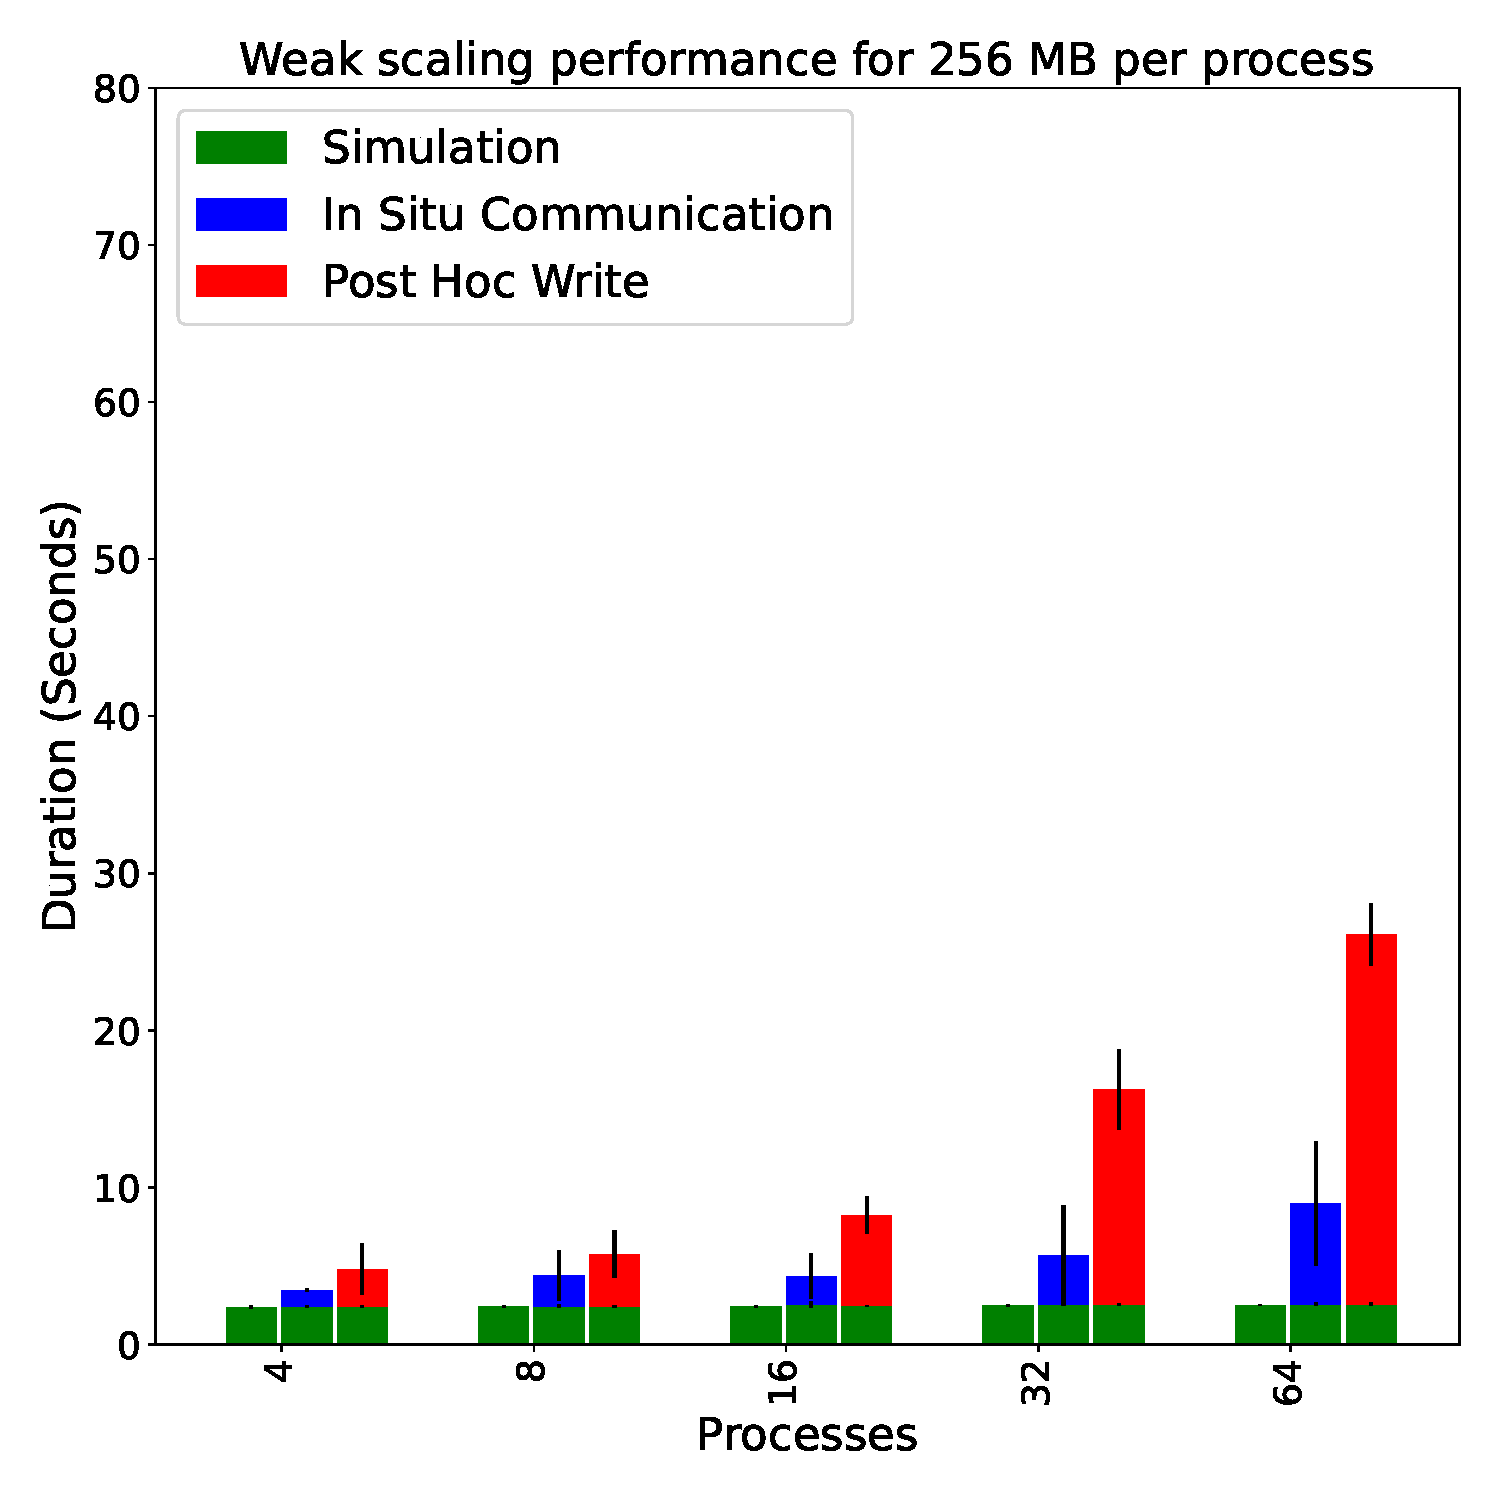
\includegraphics[width=\textwidth, height=\textwidth]{figures/256MB.pdf}
         \caption{Average simulation, communication and IO times per iteration for case: 256\,MiB per process}
         \label{fig:X256}
     \end{subfigure}
     \hfill
     \begin{subfigure}[b]{0.3\textwidth}
         \centering
         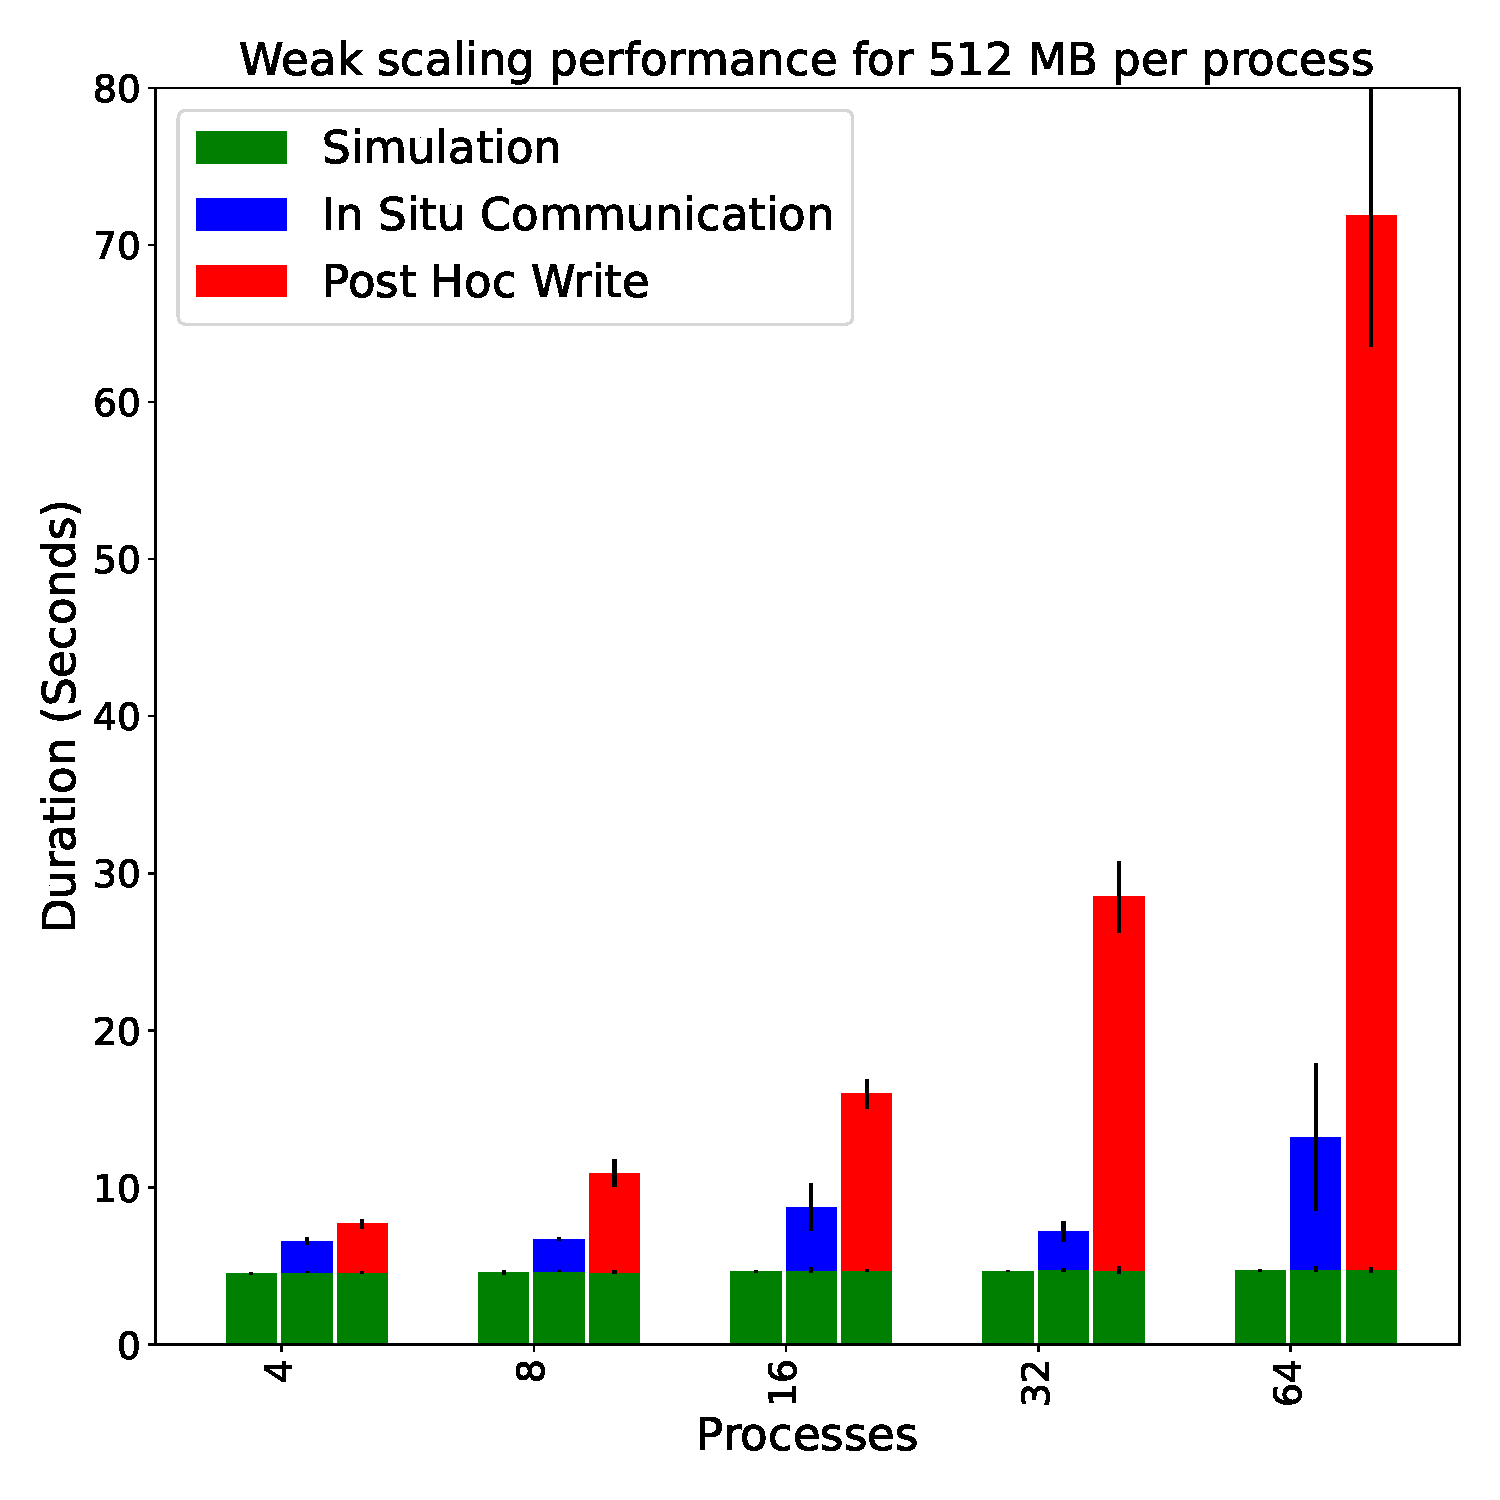
\includegraphics[width=\textwidth, height=\textwidth]{figures/512MB.pdf}
         \caption{Average simulation, communication and IO times per iteration for case: 512\,MiB per process}
         \label{fig:X512}
     \end{subfigure}
        \caption{Weak scaling average simulation, communication and IO times per iteration for 128 MiB, 256\,MiB and 512\,MiB per process for three experiments: the first bar from the left of each scale represents the baseline (simulation time without any IOs), the second shows the results for \deisa (simulation and communication time over network), and the third bar represents results for the post hoc experiment (simulation and parallel HDF5 write).}
        \label{fig:perfX1}
\end{figure}

Figure~\ref{fig:perfX1} shows the weak scaling results for the different configurations of \textbf{Experiment I}\ref{XP1}. In the first subfigure from the left: \ref{fig:X128}, we have fixed the size of the data per MPI process to 128\,MiB, to 256\,MiB in the subfigure in the middle\ref{fig:X256}, and to 512\,MiB in the subfigure in the right\ref{fig:X512}. 
The x-axis of each subfigure represents the variation of the processes for 4 to 64, and y-axis represents the duration in seconds of the different steps.
In each subfigure, we have the three cases of \textbf{Experiment I}\ref{XP1}: the first bar from the left, of each scale,  is the baseline (simulation without IO). 
The stacked bar in the middle shows results for \deisa: simulation in green, and the in situ communication over the network in blue. The last stacked bar of each scale show results for the post hoc experiment: simulation in green and parallel HDF5 \textit{write} in red.

The represented values are the mean of the maximum duration per iteration over ranks and runs. The bar errors are the standard deviation of the maximum duration per iteration over ranks and runs. 
First of all, the simulation time for all the experiments is almost the same with minimal variability, and it weak-scales perfectly when increasing the problem size.

We notice that the \deisa communication duration is less than the HDF5 write in all the experiments, which is expected, as in \deisa we just send the data over the network, whereas in post hoc, we write data to the shared PFS. 

In theory, \deisa will have better performance than post hoc,  when the aggregated network bandwidth of \dask workers is greater than the data rate transfer of the Scratch disk of Irene. Concretely, the network bandwidth is 100Gb/s, and the Scratch data rate transfer is 300GB/s. We can expect to be better than post hoc, starting at 24 worker nodes.
However, with only two worker nodes, \deisa is already slightly better than post hoc performance, in the three subfigures. This is simply explained by the fact that we never reach the theoretical disk transfer rate in real experiments.
In theory, we expect \deisa to scale perfectly as the aggregated bandwidth increases in correlation with the problem size. However, we notice that the \deisa communication times increase slightly when increasing the number of processes. 
The small variation and the variability are due to the number of communications to the \dask scheduler that may slow it down.  

The gap between in situ and post hoc performance increases when increasing the number of nodes (thus the number of \dask worker nodes). This is because the rate transfer is fixed. Thus, we face the IO bottleneck post hoc while the aggregated network bandwidth increases with the problem size.    
The variability in the red bars (HDF5 write) is likely due to sharing the parallel file system with other applications.

\begin{figure}
     \centering
     \begin{subfigure}[b]{0.3\textwidth}
         \centering
         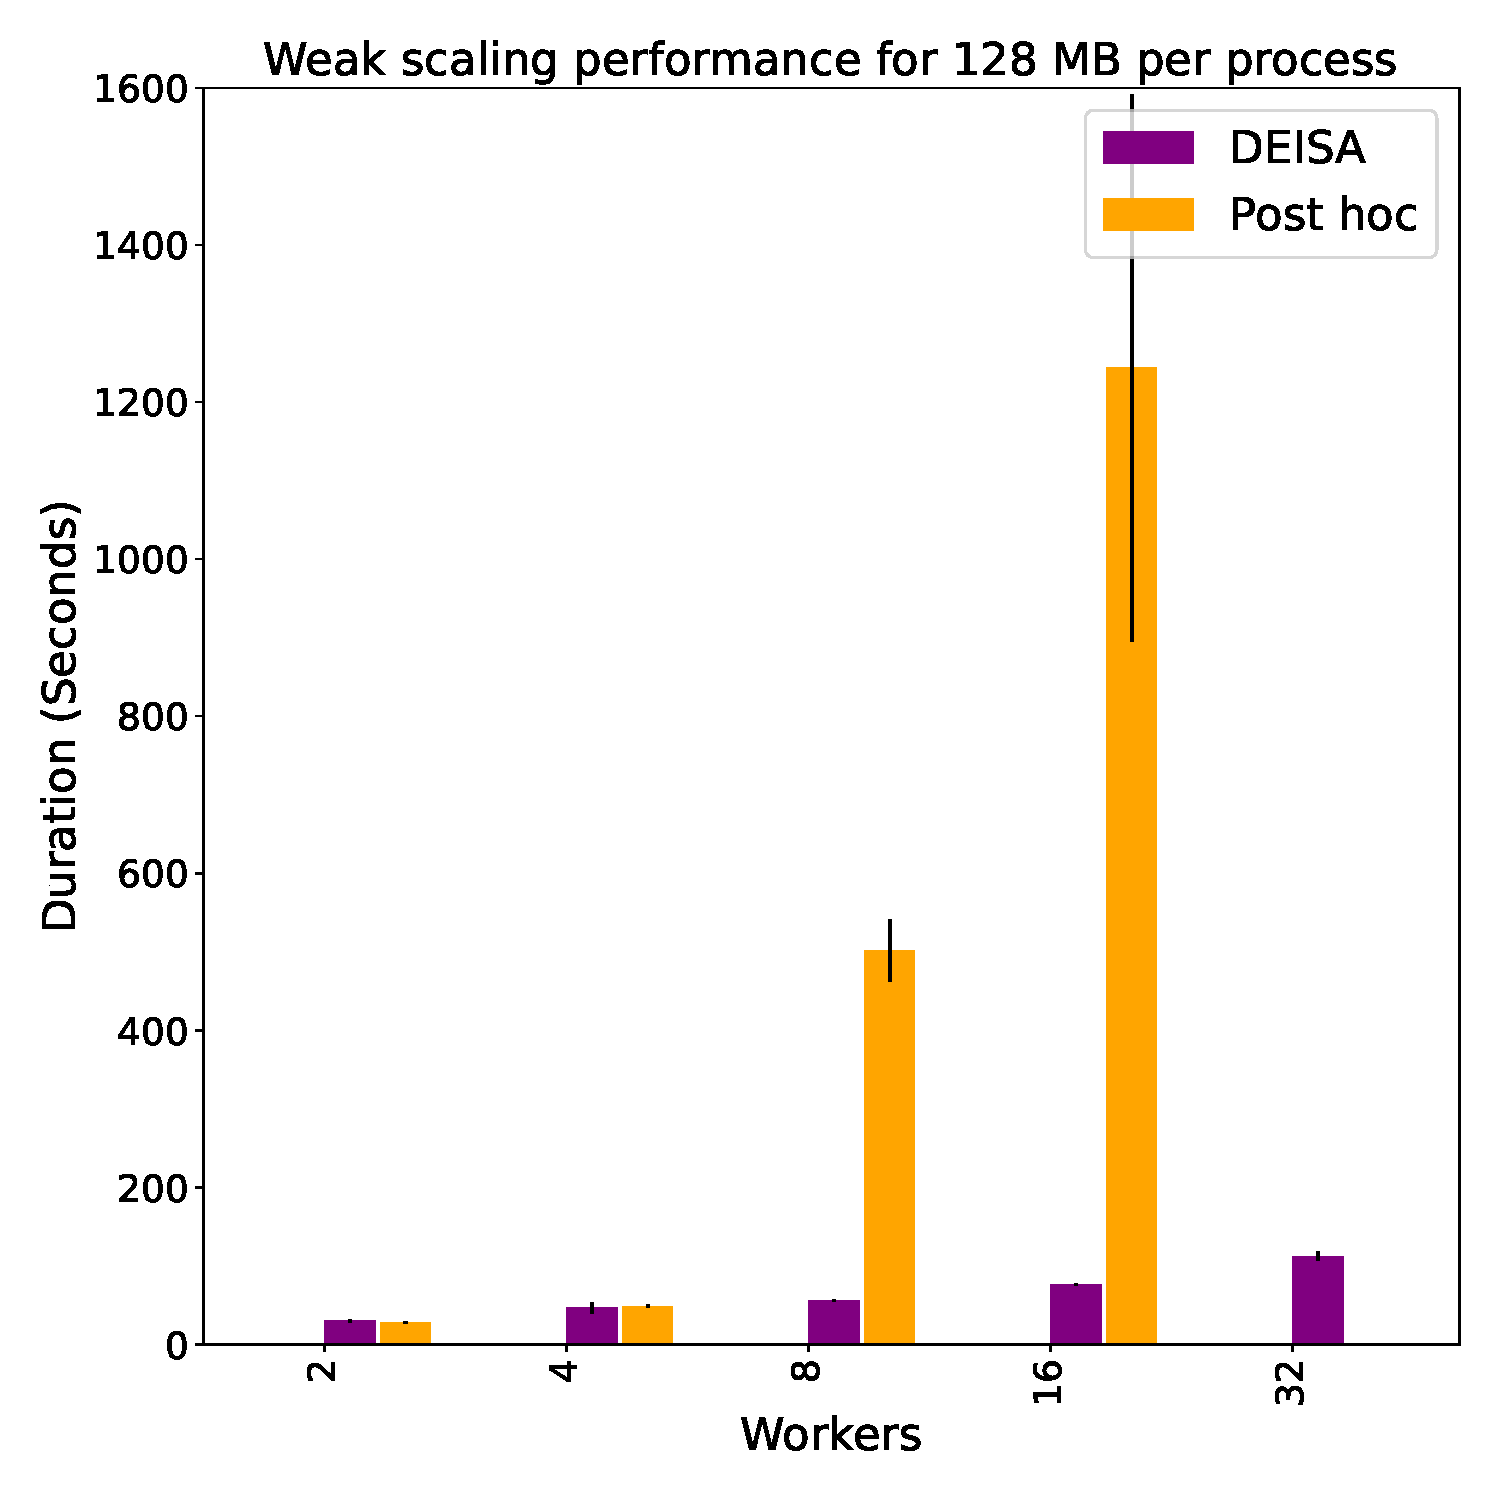
\includegraphics[width=\textwidth, height=\textwidth]{figures/128A.pdf}
         \caption{Total analytics time for case: 128\,MiB per process}
         \label{fig:A128}
     \end{subfigure}
     \hfill
     \begin{subfigure}[b]{0.3\textwidth}
         \centering
         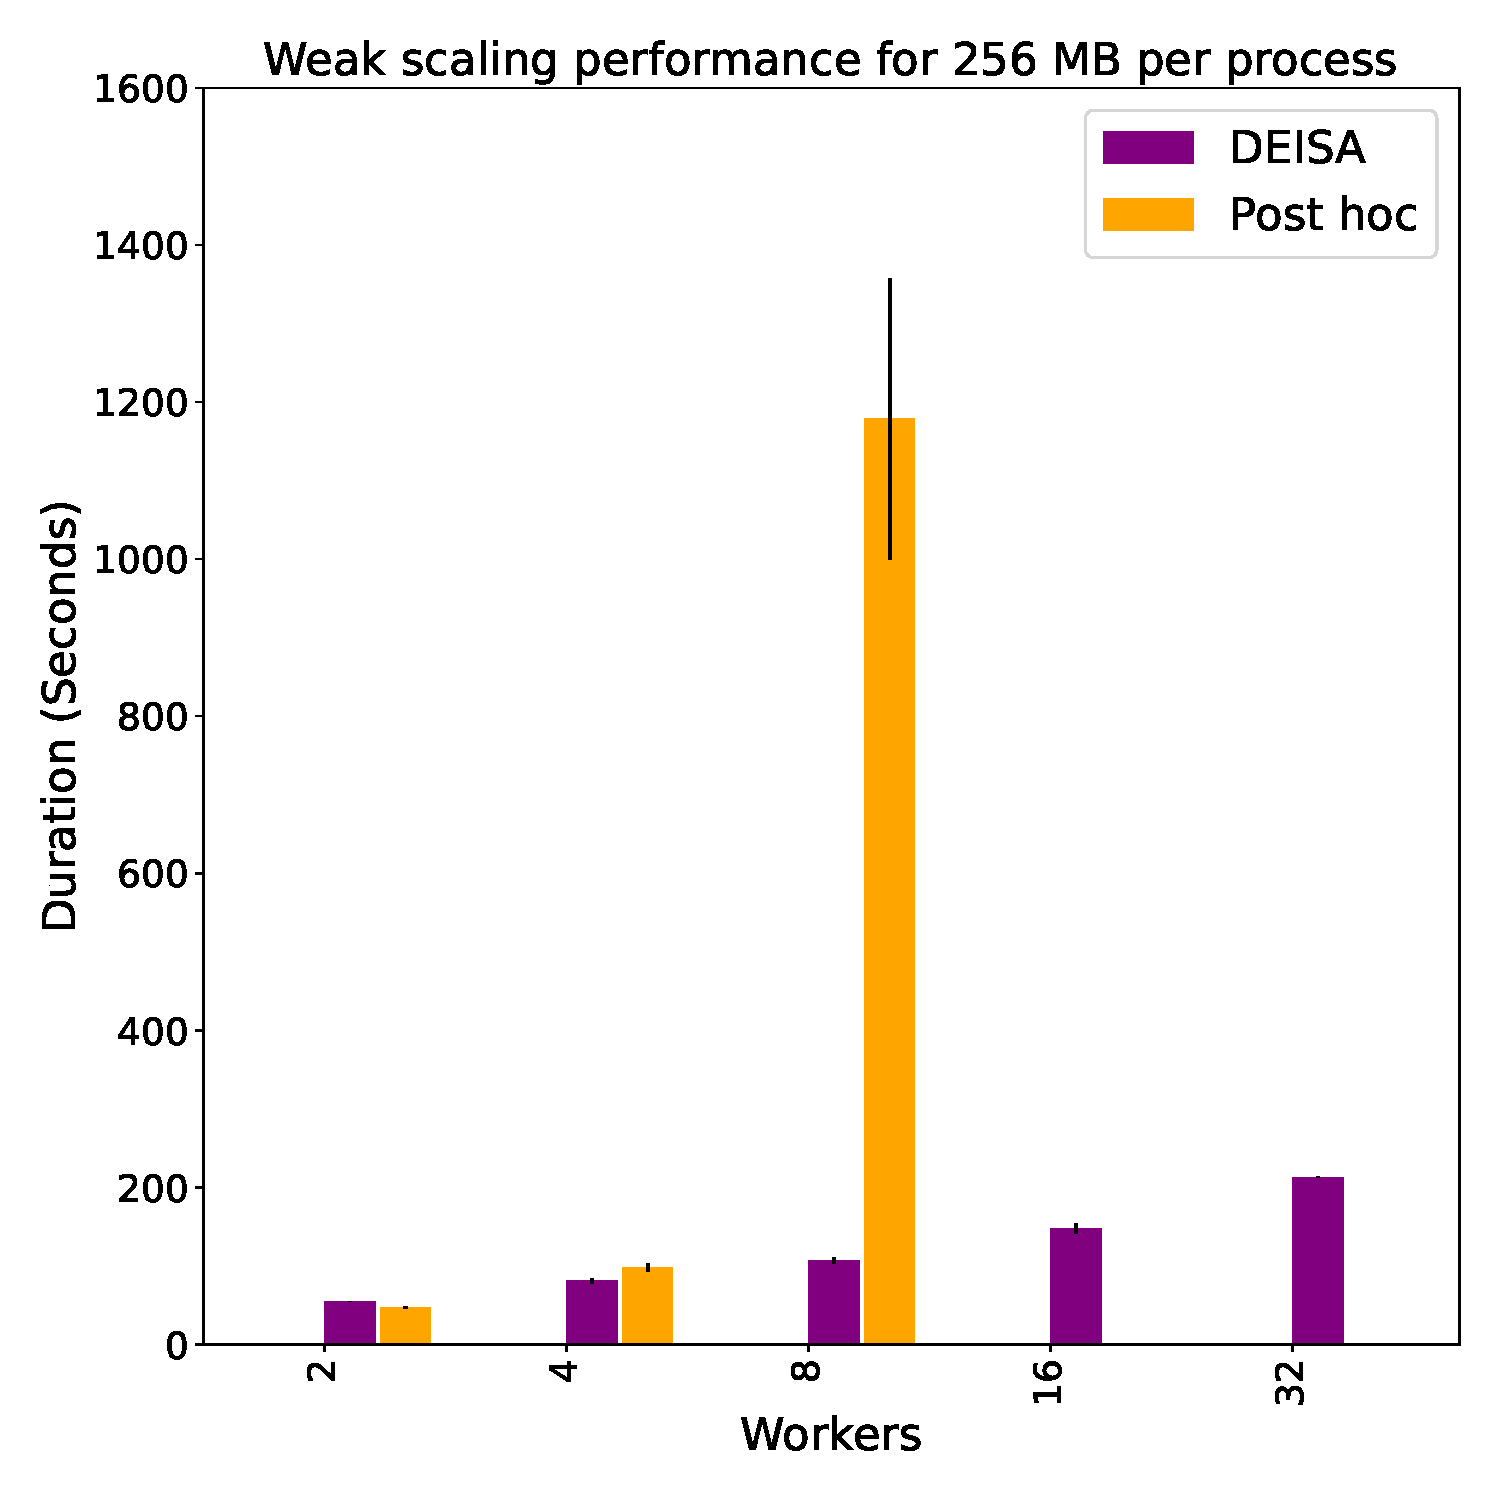
\includegraphics[width=\textwidth, height=\textwidth]{figures/256A.pdf}
         \caption{Total analytics time for the case: 256\,MiB per process}
         \label{fig:A256}
     \end{subfigure}
     \hfill
     \begin{subfigure}[b]{0.3\textwidth}
         \centering
         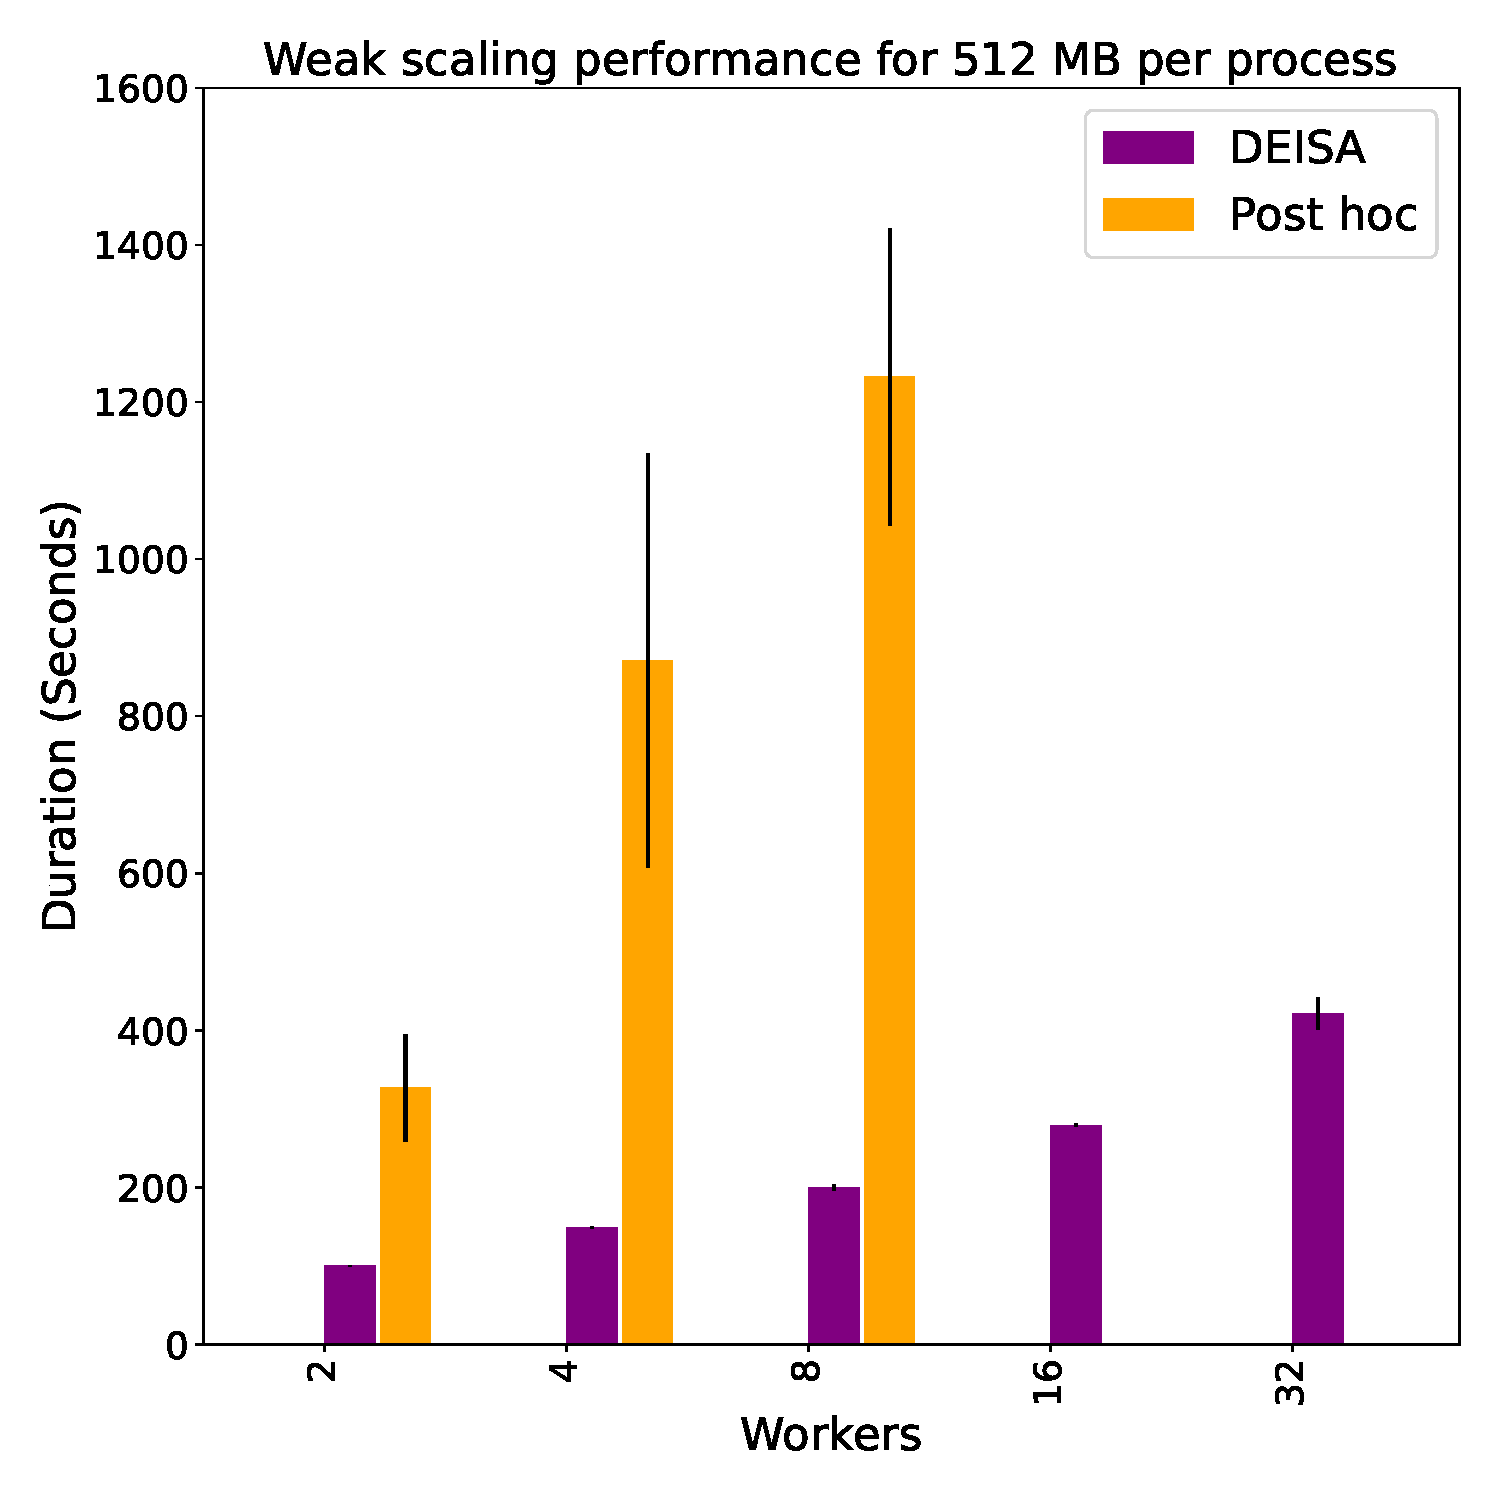
\includegraphics[width=\textwidth, height=\textwidth]{figures/512A.pdf}
         \caption{Total analytics time for case: 512\,MiB per process}
         \label{fig:A512}
     \end{subfigure}
        \caption{Weak scaling performance for the analytics. The first bar from the left shows the duration time in seconds of the in situ incremental PCA with \deisa, it includes waiting for the data to be available and the analytics duration. The second bar shows results for the post hoc version that includes both reading data from the PFS and processing it with the same algorithm.}
        \label{fig:perfA1}
\end{figure}

Figure~\ref{fig:perfA1} shows the weak scaling results for the analytics part of the different configurations of \textbf{Experiment I}\ref{XP1}. In the first subfigure from the left: \ref{fig:A128}, we have fixed the chunk size, which is the size of the data per MPI process to 128\,MiB, to 256\,MiB in the subfigure in the middle\ref{fig:A256}, and to 512\,MiB in the subfigure in the left\ref{fig:A512}. The x-axis of each subfigure represents the variation of the MPI processes from 4 to 64, equivalent to the variation of the \dask workers from 2 to 32. The y-axis represents the duration in seconds of the analytics. 
In each subfigure, we have the \deisa and the \dask analytics: the bar on the left of each scale is the \deisa analytics time that includes compute time and waiting for the data from the next step. The bar on the right of each scale shows the analytics time,  which includes reading the data from the disk and analysing the data. 
The represented values are the mean duration over the three runs. The bar errors represent the standard deviation over the three runs.       

Results for \deisa are quite good compared to post hoc. Since the analytics time includes waiting for simulation data, we can not affirm that the IPCA algorithm does not scale perfectly. The variability is also limited, which is good.

When the chunks are 128\,MiB, the post hoc results increase exponentially, starting from 8 workers to reach x25 times longer than in situ time at 16 workers. Similarly, when the chunks are 256\,MiB, with 8 workers, the analytics time increases exponentially. For 512\,MiB the scaling is linear but not better than the other sizes.
Since we are performing the exact same algorithm as in the in situ case with the exact same configurations, the only reason to have such results may be the time spent by \dask workers in reading the data. The \dask workers get the tasks at runtime; one reason may be the fact that the workers open and close the file for each \textit{read} task. 
Another reason may be the chunking of the files: we have not specified any chunking of the \pdi HDF5 plugin, so by default, no chunking is activated\cite{noauthor_pdidev_2022}. \dask may not be efficient in reading non-chunked files. 

Note that we don't have some values for the post hoc analytics experiments because the three runs crashed. The worker's and scheduler's logs show that the scheduler kills the workers after a given timeout without sending heartbeats. This is the case when the workers do long IOs. 

We repeated the experiment by activating the chunking of the HDF5 files. It is equal at each time to the local block size of an MPI process which is equal to the chunking in \dask too. 
The results are represented in Figure\ref{fig:perfA2}. Post hoc performance is clearly better with the chunking activated. 
Even if the \deisa time includes the waiting for simulation data, it weak-scales better than post hoc, and the ratio between the \deisa performance and the post hoc one increases when increasing the number of \dask workers likely because of the shared parallel file system. 

The missed values for post hoc here are due to crashes in the simulation side, likely because of the bug in HDF5~\cite{large_2023}.

\begin{figure}
     \centering
     \begin{subfigure}[b]{0.3\textwidth}
         \centering
         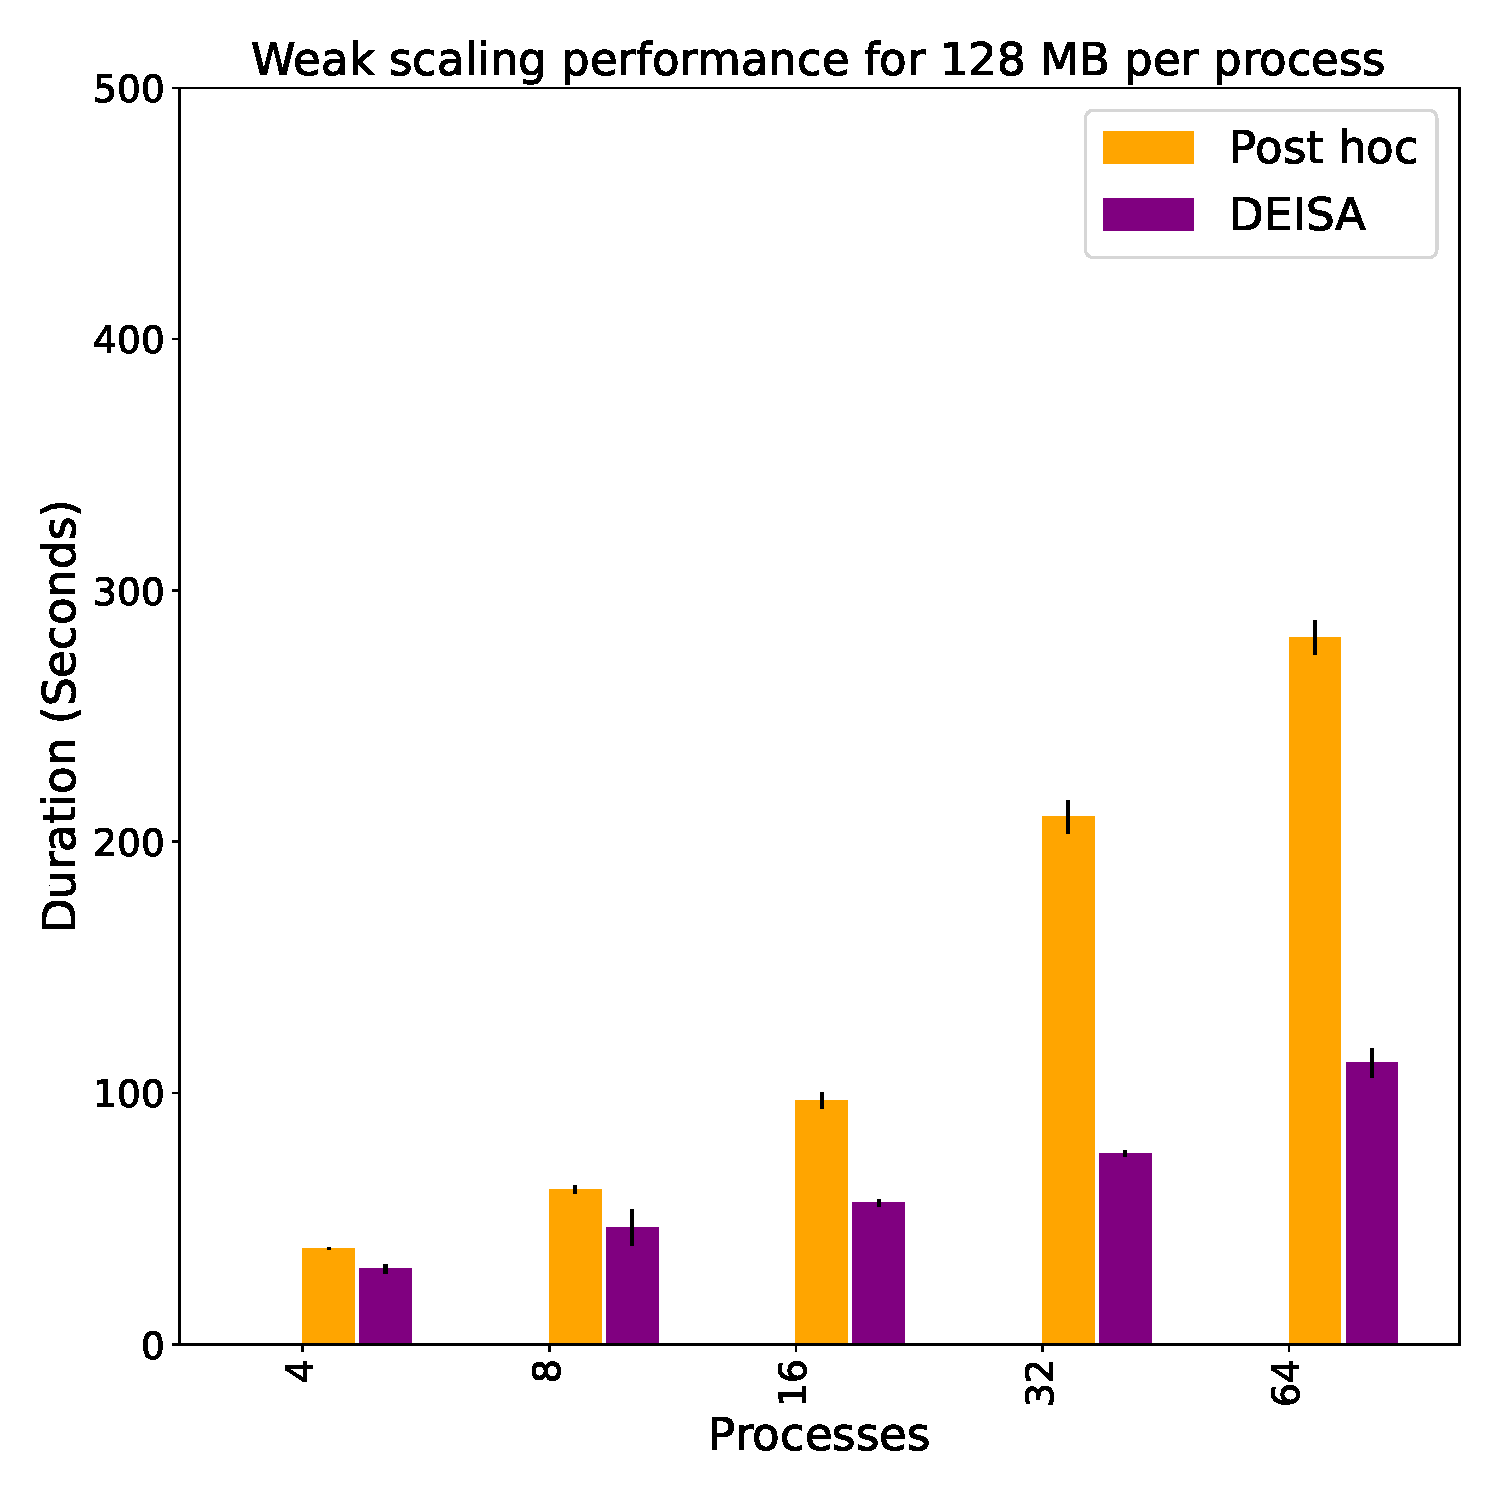
\includegraphics[width=\textwidth, height=\textwidth]{figures/128A_CH.pdf}
         \caption{Total analytics time for case: 128\,MiB per process}
         \label{fig:A128CH}
     \end{subfigure}
     \hfill
     \begin{subfigure}[b]{0.3\textwidth}
         \centering
         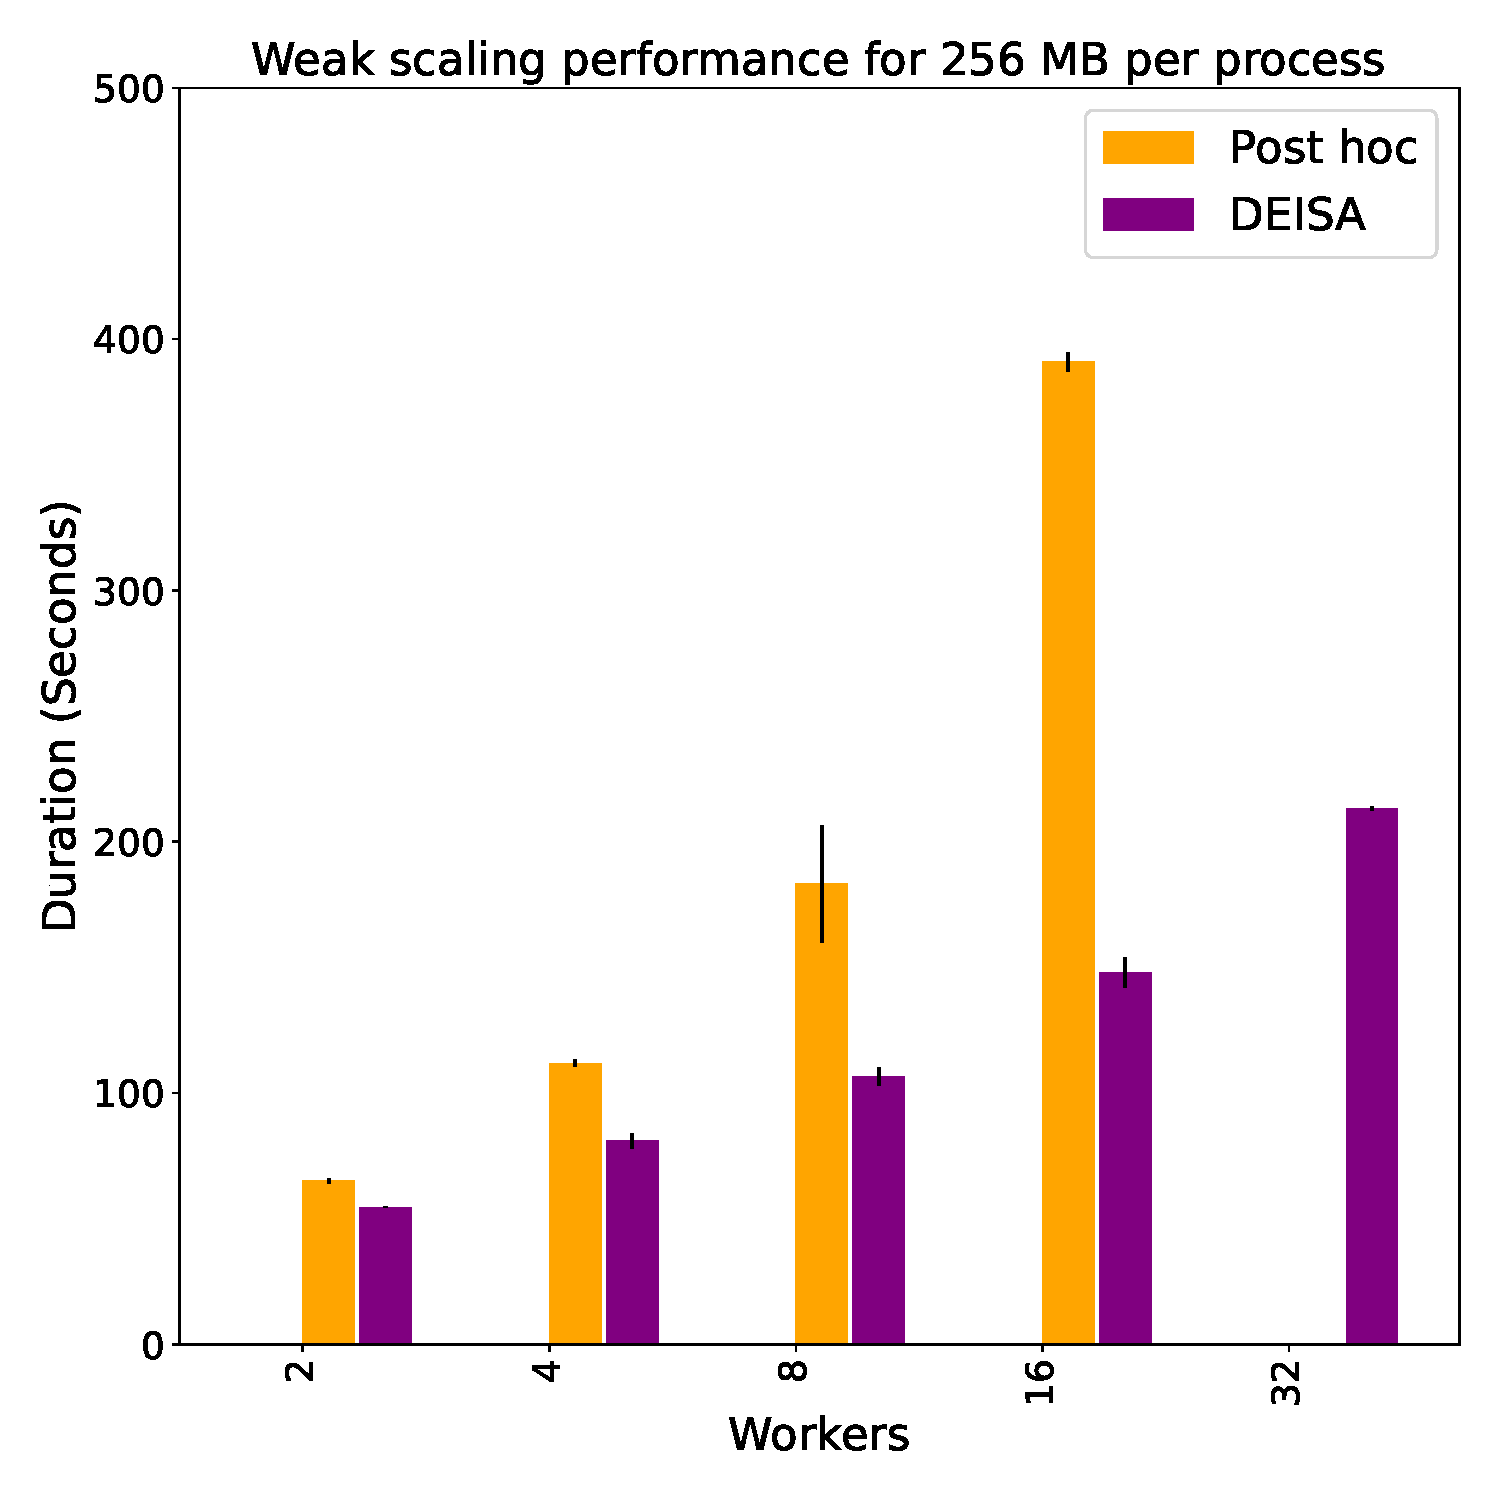
\includegraphics[width=\textwidth, height=\textwidth]{figures/256A_CH.pdf}
         \caption{Total analytics time for the case: 256\,MiB per process}
         \label{fig:A256CH}
     \end{subfigure}
     \hfill
     \begin{subfigure}[b]{0.3\textwidth}
         \centering
         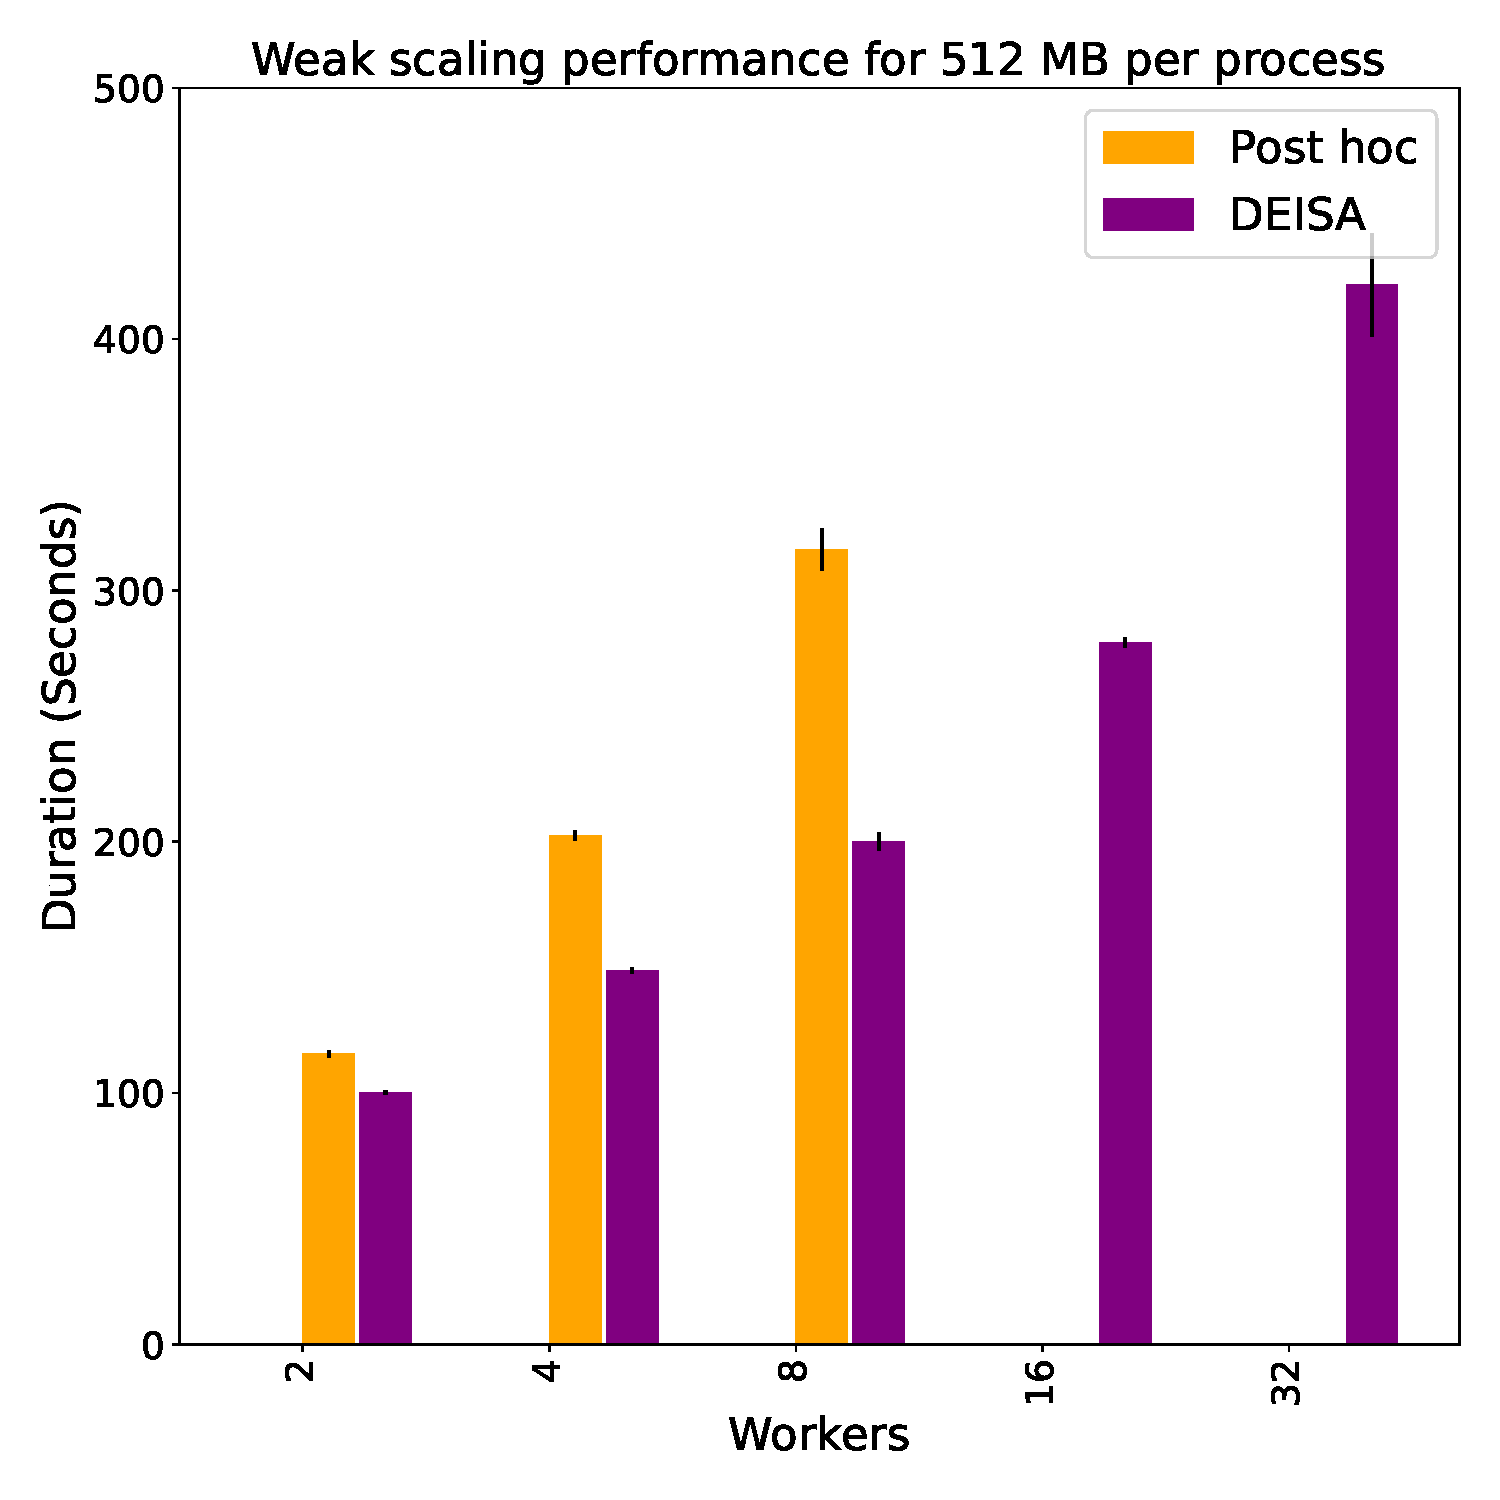
\includegraphics[width=\textwidth, height=\textwidth]{figures/512A_CH.pdf}
         \caption{Total analytics time for case: 512\,MiB per process}
         \label{fig:A512CH}
     \end{subfigure}
        \caption{Weak scaling performance for the analytics with chunking activated while writing the HDF5 file. The chunking is equal to the size of data per MPI process and the chunking in \dask. The first bar from the left shows the duration time in seconds of the in situ incremental PCA, and the second bar shows results for the post hoc version that includes both reading data from the PFS and processing it with the same algorithm.}
        \label{fig:perfA2}
\end{figure}

Figure~\ref{fig:taskstreamdask} and Figure~\ref{fig:taskstreamdeisa} show the two stream tasks generated by \dask for the Incremental PCA, in the configuration: 64 MPI processes, 32 workers and 128\,MiB, \dask post hoc version in the first and \deisa in situ version in the second. The x-axis represents the time, and the y-axis represents the cores of the workers. 
The small colored patches are tasks. Each color represents a type of task. We will not detail more those task streams, but they can be found online\footnote{https://gitlab.maisondelasimulation.fr/agueroud/phd\_xp}. 
The colours in the task stream are not similar, as the submitted task graphs are different. In the in situ version we do not perform reads for instance.
In the post hoc stream task, \dask generated more tasks compared to the in situ version because reading data from disk are considered as tasks so they are also included in the count. 
In both figures, we can notice that there are 10 steps (iterations). The algorithm computes the PCA incrementally. It submits a task graph for each iteration.


\begin{figure}[ht]\centering
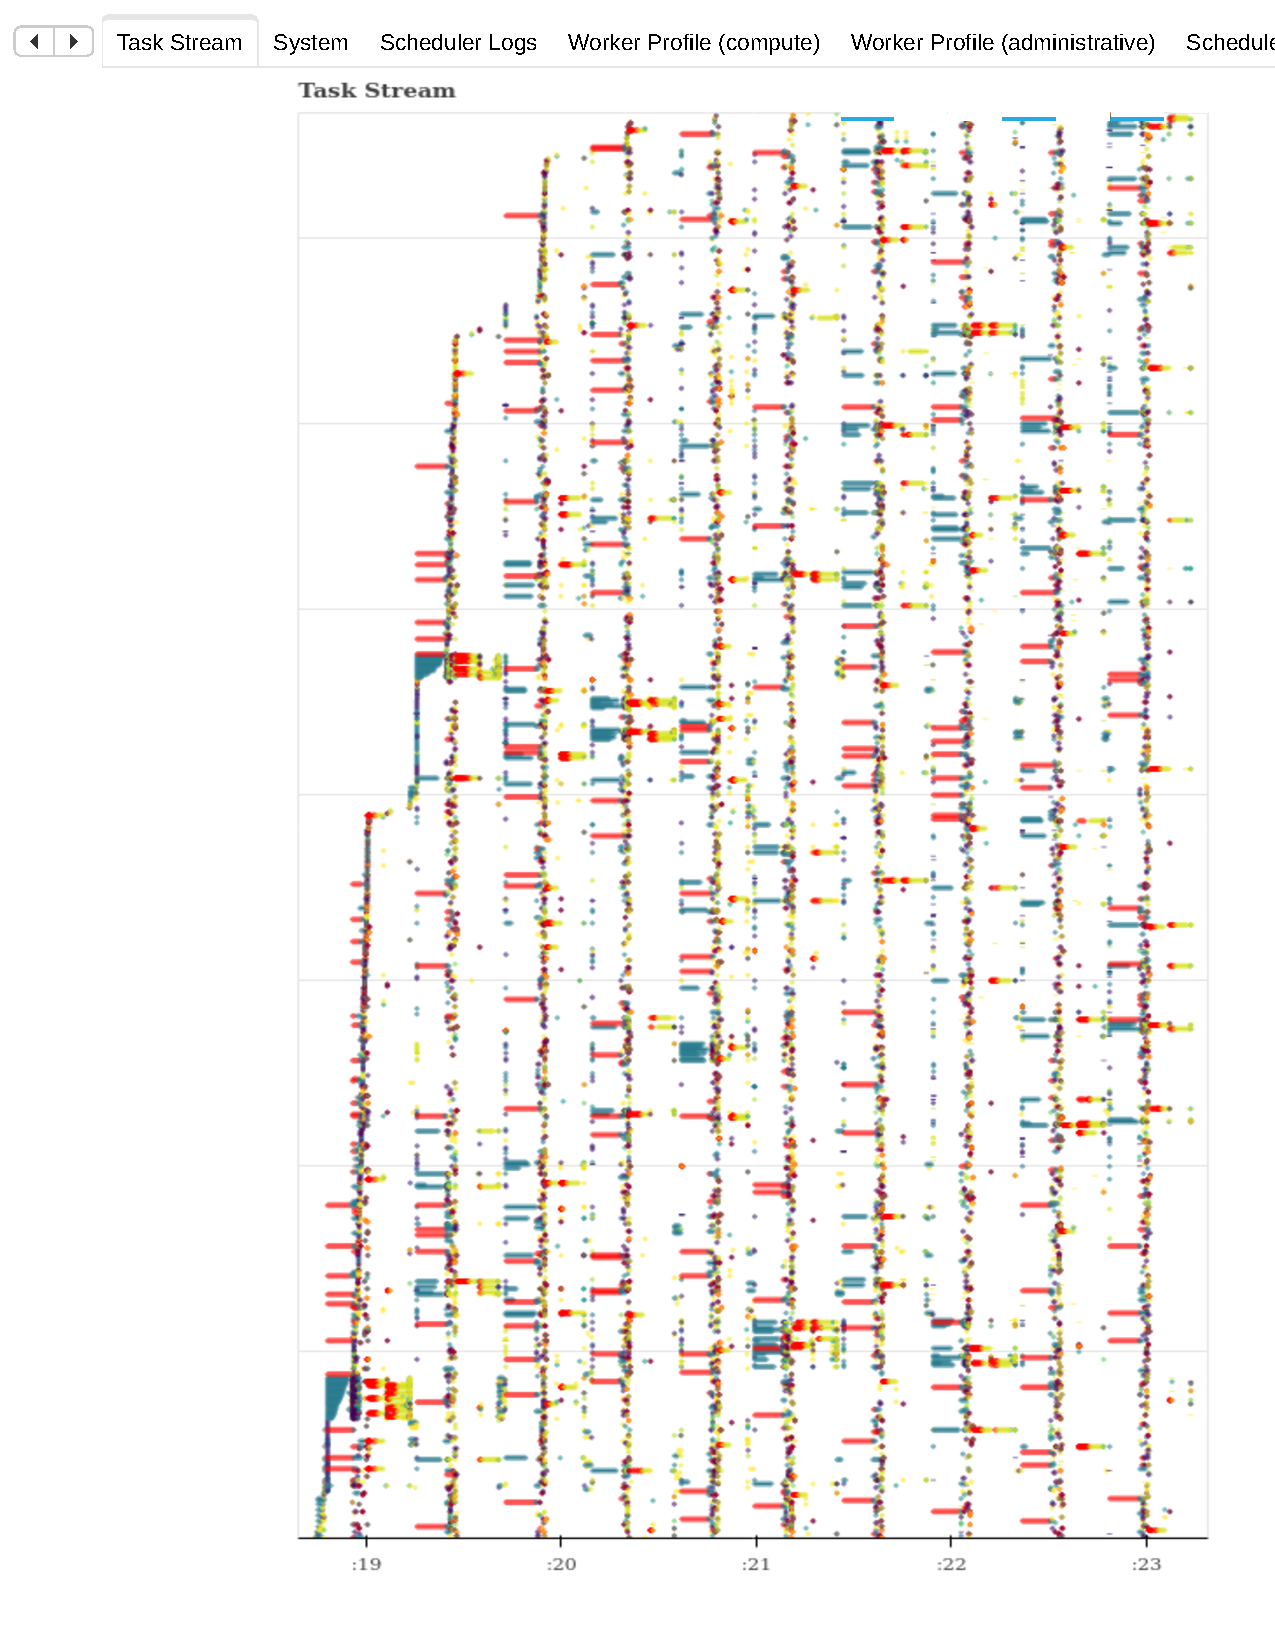
\includegraphics[width=\columnwidth]{figures/P64_W32_D128_DASK_CHUNK.pdf}
\caption{Task stream generated by \dask for post hoc incremental IPCA with chunking activated for 64 processes, 32 workers and 128\,MiB per process. 
    Number of tasks: 11565,
    Compute time: 3017.67s, 
    Deserialize time: 25.39s,
    Disk-read time: 64.45ms,
    Transfer time: 2709.88s.}
\label{fig:taskstreamdask}
\end{figure}


\begin{figure}[ht]\centering
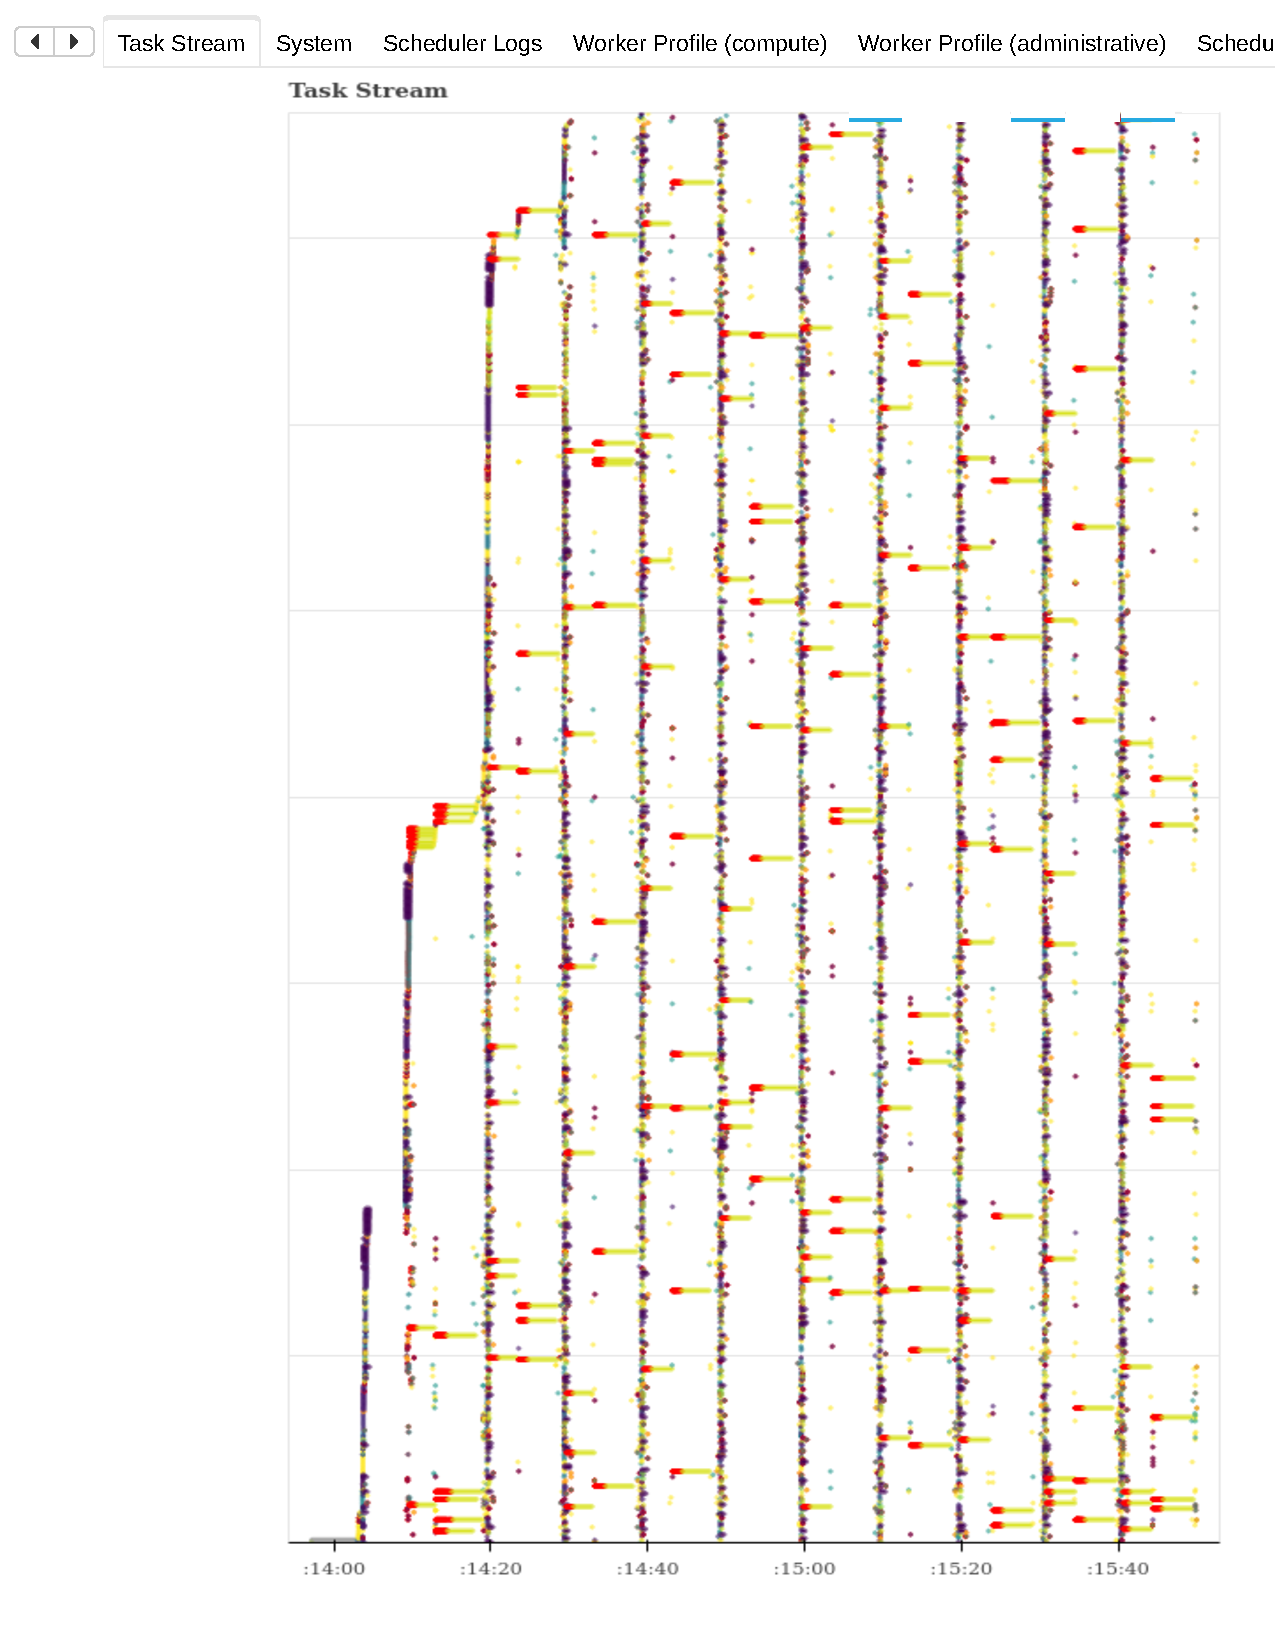
\includegraphics[width=\columnwidth]{figures/P64_W32_D128_DEISA.pdf}
\caption{Task stream generated by \dask with in situ analytics enabled for the IPCA, for 64 processes, 32 workers and 128\,MiB per process.
    number of tasks: 9269,
    compute time: 1104.79s,
    deserialize time: 5.89s,
    disk-read time: 63.47ms,
    transfer time: 1007.39s.}
\label{fig:taskstreamdeisa}
\end{figure}


\subsubsection{Experiment II}\label{XP2}

In this Experiment we perform a very detailed study about the variability and performance of \deisa communications and how they affect the scheduler performance. This section has already been presented in paper~\cite{deisa}.


\begin{table}[tb]
\centering
\begin{tabular}{||ll||}
\hline
 Parameter                         & Value \\
\hline
 MPI nodes / Dask worker node      & 4 \\
 MPI process / MPI node            & 32  \\
 Dask worker / Dask worker node    & 16  \\
 Thread / Dask worker              & 2  \\
 MPI process / Dask worker         & 8 \\
 Data size / MPI process           & 128\,MiB \\
 Data size / MPI node              & 4\,GiB \\
 Mean data size / Dask worker node & 16\,GiB \\
\hline
\end{tabular}
\caption{\label{parameters2}Fixed parameters used in Experiment II~\ref{XP2}}
\end{table}


\begin{table}[tb]\centering
\begin{tabular}{||ccccc||}
\hline
 Configuration   &             XP2:{1\,MiB:128}     & XP2:{1\,MiB:512}    & XP2:{256\,MiB:128} & XP2:{256\,MiB:512} \\
\hline\hline
 Data size / MPI process            & 1\,MiB        & 1\,MiB        & 256\,MiB       & 256\,MiB   \\
 Total nodes                        & 6             & 21            & 6             & 21 \\
 MPI node                           & 4             & 16            & 4             & 16\\
 \dask worker nodes                 & 1             & 4             & 1             & 4\\
 client \& scheduler node           & 1             & 1             & 1             & 1\\
 Global data size                   & 128\,MiB      & 512\,MiB      & 32\,GiB       & 128\,GiB \\
 Data size / MPI node               & 32\,MiB       & 32\,MiB       & 8\,GiB        & 8\,GiB   \\
 Generated tasks                    & 15330         & 55330         & 15210         & 55150\\
\hline\hline
\end{tabular}
\caption{\label{configXP2}Four configurations used for Experiment II~\ref{XP2}}
\end{table}

\begin{figure}[tb]\centering
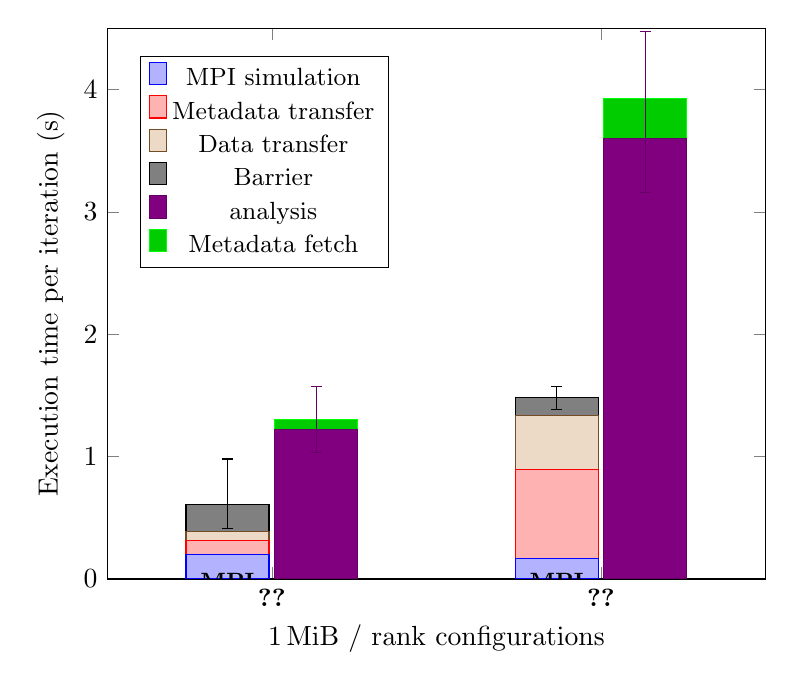
\begin{tikzpicture}[
/pgfplots/every axis/.style={ % <- added /pgfplots/ 
    ybar stacked,
    ymin=0,
    ymax=4.5,
    ytick={0, 1, 2, 3, 4},
    symbolic x coords={411, 1641},
    bar width=30pt,
    legend style={font=\small, at={(0.05,0.95)},anchor=north west},
    ylabel={Execution time per iteration (s)},
    xlabel={1\,MiB / rank configurations},
    xtick=data,
    xticklabels={\ref{XP2.1.128},\ref{XP2.1.512}},
    x tick label style={font=\small,},
    hide axis,
    width=.82\columnwidth,
    enlarge x limits={rel=0.5},
    point meta=explicit symbolic,
  }, 
]
\begin{axis}[bar shift=-16pt, hide axis=false]
\legend{MPI simulation, Metadata transfer, Data transfer, Barrier, \dask analysis, Metadata fetch}
\addplot coordinates { (411,0) (1641,0) };
\addplot coordinates { (411,0) (1641,0) };
\addplot coordinates { (411,0) (1641,0) };
\addplot coordinates { (411,0) (1641,0) };
\addplot coordinates { (411,0) (1641,0) };
\addplot coordinates { (411,0) (1641,0) };
\end{axis}

%%%%%%%%%%%%%% 1M %%%%%%%%%%%%%%%%%%%%%%%%%%%%%%%%%%%%%%%%%%%%%%%%%

%meansimu =   [0.20378826092928648,  0.16849265048716688]
%meandask =  [1.2227224971564417, 3.60005530453701]
%meanputq= [0.11280882632812943,  0.7232108102396827]
%meangetq= [0.08205931478490432,  0.32900929676058394]
%meanscatter= [0.07447400204512178,  0.4456939545007496]
%meanbar= [0.21443583569608413,  0.1472610141856876]

%iter =  [Max( MPI:0.6073631280990716, Dask: 1.304781811941346 ),Max ( MPI: 1.486193363804432, Dask : 3.929064601297594 )]
% 2%*iter = [0.02609563623882692, 0.07858129202595188]

%%%%%%%%%%%%%%%%%%%%%%%%%%%%%%%%%%%%%%%%%%%%%%%%%%%%%%%%%%%%%%%%%%%%%%%%%%%

%%%% MPI %%%%
\begin{axis}[xshift=-16pt]
\node[coordinate,pin={{\footnotesize\bfseries MPI}}] at (411,-.45) {};
\node[coordinate,pin={{\footnotesize\bfseries MPI}}] at (1641,-.45) {};

%stdsimu =  [0.028907557788677447,  0.00656858080088586] : [0.02609563623882692, 0.07858129202595188]
%Min simu =  [0.17287868517973948,  0.16206971241592782]
%Mean simu =  [0.20378826092928648,  0.16849265048716688] 
%Max simu [0.23015613693451087,  0.17519777858422003]


\addplot+[error bars/.cd, y dir=both, y explicit]  %simu
         coordinates { (411,0.203)
                       %+- (,0.00656858080088586) % < 0.02609563623882692
                       (1641,0.168)
                       % +- (,0.00656858080088586) % < 0,0.02972386727
                     };
%stdputq =  [0.005781409824694809,  0.009123255592682601] : < [0.02609563623882692, 0.07858129202595188]
%Min putq =  [0.10689240859187521,  0.7171006665419668]
%Mean putq =  [0.11280882632812943,  0.7232108102396827]
%Max putq [0.11844503826546315,  0.733697799782135]


\addplot+[error bars/.cd, y dir=both, y explicit]  %putq
         coordinates { (411,0.11280882632812943)
                       % +- (,0.005781409824694809) % < 0.02609563623882692
                       (1641,0.7232108102396827)
                       % +- (,0.009123255592682601) % < 0.07858129202595188
                      };
%stdscatter =  [0.022278990461730694, 0.06619416442538288] : < [0.02609563623882692, 0.07858129202595188]
%Min scatter =  [0.05815409594345056,  0.4070897154490467]
%Mean meanscatter =  [0.07447400204512178,  0.4456939545007496]
%Max scatter [0.0998560024370363,  0.5221270809265661]


\addplot+[error bars/.cd, y dir=both, y explicit]  %scatter
         coordinates { (411,0.07447400204512178)
                       %+- (,0.022278990461730694)
                       (1641,0.4456939545007496)
                       %+- (,0.06619416442538288)
                      };
%stdbar =  [0.3250447445341635,  0.09527162041058722] : > [0.02609563623882692, 0.07858129202595188]
%Min bar =  [0.024776848883675484, 0.046745352296341025]
%Mean bar =  [0.21443583569608413,  0.1472610141856876]
%Max bar [0.5897580874584492,  0.23623748330203398]

\addplot+[error bars/.cd, y dir=both, y explicit]  %bar
         coordinates { (411,0.21443583569608413)
                       += (,0.375322251762365) -= (,0.18965898681240864)
                       (1641,0.1472610141856876)
                       += (,0.08897646911634638) -= (,0.10051566188934657)
                      };
\addplot coordinates { (411,0)     (1641,0)     }; %dask
\addplot coordinates { (411,0)     (1641,0)     }; %getq
\end{axis}

%%%% Dask %%%%
\begin{axis}[xshift=16pt] 
\node[coordinate,pin={{\footnotesize\bfseries \dask}}] at (411,-.45) {};
\node[coordinate,pin={{\footnotesize\bfseries \dask}}] at (1641,-.45) {};
\addplot coordinates { (411,0)     (1641,0)     }; %simu
\addplot coordinates { (411,0)     (1641,0)     }; %putq
\addplot coordinates { (411,0)     (1641,0)     }; %scatter
\addplot coordinates { (411,0)     (1641,0)     }; %bar
%stddask =  [0.3015011760477324, 0.7588320784454731] : > [0.02609563623882692, 0.07858129202595188]
%Min dask =  [1.0339068029231082, 3.157302851245428]
%Mean dask =  [1.2227224971564417, 3.60005530453701]
%Max dask [1.5704373405573682, 4.476262671329702]


\addplot+[error bars/.cd, y dir=both, y explicit]  %dask
         coordinates { (411,1.2227224971564417)
                       += (,0.3477148434009265) -= (,0.18881569423333344)
                       (1641,3.60005530453701)
                       += (,0.8762073667926922) -= (,0.4427524532915821)
                      };
%stdgetq =  [0.0015614752884921415, 0.012205066604482485] : < [0.02609563623882692, 0.07858129202595188]
%Min getq =  [0.08025651518255472,  0.3181074700421757]
%Mean getq =  [0.08205931478490432,  0.32900929676058394]
%Max getq [0.0829860181806402,  0.3421949552009917]


\addplot+[error bars/.cd, y dir=both, y explicit]  %getq
         coordinates { (411,0.08205931478490432)
                       % +- (,0.0015614752884921415) % < 0,00807149734339
                       (1641,0.32900929676058394)
                       % +- (,0.012205066604482485) % < 0,0263540142663
                      };
\end{axis}

\end{tikzpicture}



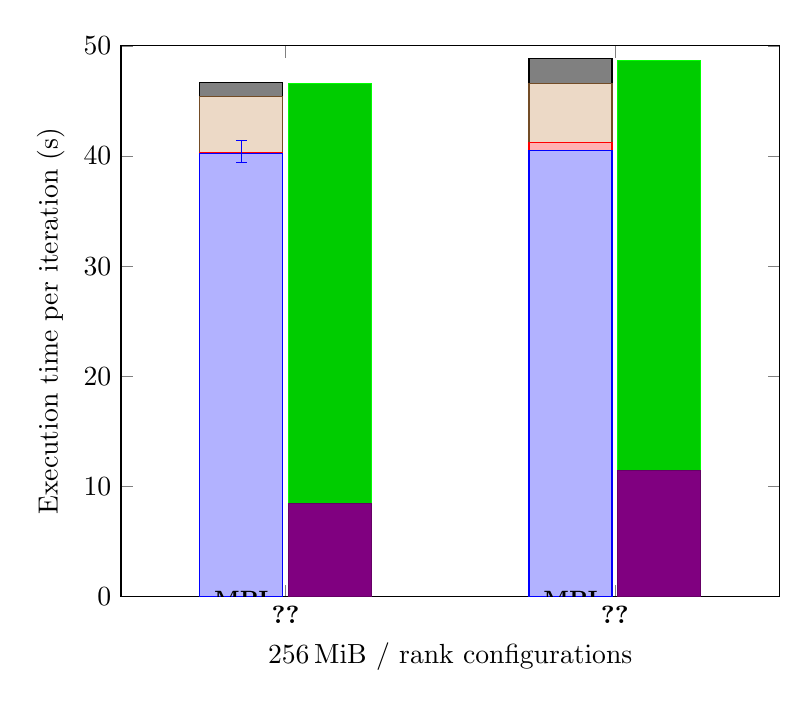
\begin{tikzpicture}[
/pgfplots/every axis/.style={ % <- added /pgfplots/ 
    ybar stacked,
    ymin=0,
    ymax=50,
    ytick={0, 10, 20, 30, 40, 50},
    symbolic x coords={ 41256, 164256},
    bar width=30pt,
    %legend style={font=\small, at={(0.05,0.9)},anchor=south east},
    ylabel={Execution time per iteration (s)},
    xlabel={256\,MiB / rank configurations},
    xtick=data,
    xticklabels={\ref{XP2.256.128},\ref{XP2.256.512}},
    x tick label style={font=\small,},
    hide axis,
    width=.82\columnwidth,
    enlarge x limits=0.5,
    point meta=explicit symbolic,
  },
]
\begin{axis}[bar shift=-16pt, hide axis=false]
\addplot coordinates { (41256,0) (164256,0) };
\addplot coordinates { (41256,0) (164256,0) };
\addplot coordinates { (41256,0) (164256,0) };
\addplot coordinates { (41256,0) (164256,0) };
\addplot coordinates { (41256,0) (164256,0) };
\addplot coordinates { (41256,0) (164256,0) };
\end{axis}

%%%%%%%%%%%%%%%%%% 256M %%%%%%%%%%%%%%%%%%%%%%%%%%%%%%%%%%%%%%%%

%meansimu =  [40.19396744045631, , 40.474843232321064]
%meandask =  [8.410617398468917,  11.448131603119826]
%meanputq= [0.0795850563008192,  0.7631853370359067]
%meangetq= [38.19960798663777, 37.22121849190444]
%meanscatter= [5.147044166001099,  5.316233275613153]
%meanbar= [1.253565882761298,  2.259944601142744]


%MPI iter =  [46.67603649275399,  48.81615962772145]
%Dask  = [46.61022538510669, 48.669350095024264]
%iter =  [Max( MPI, Dask: ),Max ( MPI: , Dask :  )] = 
%iter = MPI iter = [46.67603649275399,  48.81615962772145]
% 2%*iter = [0.9322045077021338, 0.9733870019004853]

%%%%%%%%%%%%%%%%%%%%%%%%%%%%%%%%%%%%%%%%%%%%%%%%%%%%%%%%%%%%

%%%% MPI %%%%
\begin{axis}[xshift=-16pt]
\node[coordinate,pin={{\footnotesize\bfseries MPI}}] at (41256,-5) {};
\node[coordinate,pin={{\footnotesize\bfseries MPI}}] at (164256,-5) {};
%stdsimu =  [1.0833717427874794,  0.4051487721548612] : [>0.9322045077021338, <0.9733870019004853]
%Min simu =  [39.44312698278668,  40.13795151070883]
%Mean simu =  [40.19396744045631, 40.474843232321064]
%Max simu [41.43591711969384,  40.924400287337676]

\addplot+[error bars/.cd, y dir=both, y explicit]  %simu
         coordinates { (41256,40.19396744045631)
                       += (,1.2419496792375284) -= (,0.7508404576696321)
                       (164256,40.474843232321064) 
                       %+- (,0.4051487721548612) % < 0.976323192554
                      };
%stdputq =  [0.007874413545552569, 0.07190917364509905]< [0.9322045077021338, 0.9733870019004853]
%Min putq =  [0.07086614267359437, 0.6901729620151968]
%Mean putq =  [0.0795850563008192,  0.7631853370359067]
%Max putq [0.08617874621711508,  0.8339380437080308]

\addplot+[error bars/.cd, y dir=both, y explicit]  %putq
         coordinates { (41256,0.0795850563008192)
                       % +- (,0.007874413545552569) % < 0.933520729855
                       (164256,0.7631853370359067) 
                       %+- (,0.07190917364509905) % < 0.976323192554
                      };
%stdscatter =  [0.22428716130564308,  0.24283345436052847] <[0.9322045077021338, 0.9733870019004853]
%Min scatter =  [4.8977906801026165,  5.168739588378514
%Mean meanscatter =  [5.147044166001099,5.316233275613153]
%Max scatter [5.332574566903986,  5.5965044415901275]

\addplot+[error bars/.cd, y dir=both, y explicit]  %scatter
         coordinates { (41256,5.147044166001099)
                       % +- (,0.22428716130564308) % < 0.933520729855
                       (164256,5.316233275613153)
                       % +- (,0.24283345436052847) % < 0.976323192554
                       };
%stdbar =  [0.0890767570792701,  0.6896973362478515] < [0.9322045077021338, 0.9733870019004853]
%Min bar =  [1.1664388556512222, 1.747406680871677]
%Mean bar =  [1.253565882761298,  2.259944601142744]
%Max bar [1.3444720780314583,  3.044097142989756]
\addplot+[error bars/.cd, y dir=both, y explicit]  %bar
         coordinates { (41256,1.253565882761298)
                       % +- (,0.0890767570792701) % < 0.933520729855
                       (164256,2.259944601142744)
                       % +- (,0.6896973362478515) % < 0.976323192554
                       };
\addplot coordinates { (41256,0)     (164256,0)     }; %dask
\addplot coordinates { (41256,0)     (164256,0)     }; %getq
\end{axis}

%%%% Dask %%%%
\begin{axis}[xshift=16pt] 
\node[coordinate,pin={{\footnotesize\bfseries \dask}}] at (41256,-5) {};
\node[coordinate,pin={{\footnotesize\bfseries \dask}}] at (164256,-5) {};
\addplot coordinates { (41256,0)     (164256,0)     }; %simu
\addplot coordinates { (41256,0)     (164256,0)     }; %putq
\addplot coordinates { (41256,0)     (164256,0)     }; %scatter
\addplot coordinates { (41256,0)     (164256,0)     }; %bar
%stddask =  [0.11870514435554211,  0.5837459627450405] < [0.9322045077021338, 0.9733870019004853]
%Min dask =  [8.329631023703971, 10.896099947574031]
%Mean dask =  [8.410617398468917, 11.448131603119826]
%Max dask [8.54688018762196,  12.059117784025148]

\addplot+[error bars/.cd, y dir=both, y explicit]  %dask
         coordinates { (41256,8.410617398468917)
                       % +- (,0.11870514435554211) % < 0.933520729855
                       (164256,11.448131603119826)
                       % +- (,0.5837459627450405) % < 0.976323192554
                       };
%stdgetq =  [0.8944936599264665,  0.05439716415244653] < [0.9322045077021338, 0.9733870019004853]
%Min getq =  [37.65883787051361,  37.182585414266214]
%Mean getq =  [38.19960798663777,  37.22121849190444]
%Max getq [39.23209190231541,  37.28342635212984]

\addplot+[error bars/.cd, y dir=both, y explicit]  %getq
         coordinates { (41256,38.19960798663777)
                       % +- (,0.8944936599264665) % < 0.933520729855
                       (164256,37.22121849190444)
                       % +- (,0.05439716415244653) % < 0.976323192554
                       };
\end{axis}

\end{tikzpicture} 


\caption{\label{XP2_time}Detailed timing per time step for \deisa with 1 or 256\,MiB /rank and 128 or 512 processes (6 or 21 nodes, respectively).
For each configuration, the left bar shows the timing for the MPI side, and the right timings for \dask side}
\end{figure}

Those experiments have been done on the Ruche cluster, where we have used the same mini-app and analytics as the previous experiment.
We investigate the performance of \deisa in depth when either the data size or computer resources vary. Those two parameters are important because they may affect the \dask performance negatively. 

To show this impact we vary the size of the data per MPI process from 1\,MiB to 256\,MiB, and we use either 128 or 512 MPI processes.
The size of the data per MPI process corresponds to the size of the chunks in the \dask analytics, and the number of MPI processes is the number of bridges connected to the scheduler.

Table~\ref{configXP2} summarizes the four configurations tested, and Figure~\ref{XP2_time} presents the average execution time over 3 runs of 10 iterations as well as an error bar representing the min and max values when standard deviation exceeds 2\%. We excluded the first iteration here as it may include initialization time.

On MPI side, we identify the compute time, the time to transfer the data from \deisa bridge to \dask workers, and that to send the required metadata to the scheduler.
We also measure the duration of a barrier inserted just after these communications.
This barrier captures the time required to re-synchronize the processes after potentially differing time in the communications.
Without it, this time would be counted as part of the computation time.

On \dask side, we identify the time required by \deisa adapter to gather all metadata from the scheduler on one hand and the time required for the submission and actual execution of the task graph on the other hand.

At 1\,MiB/process, the MPI simulation executes much faster than the analysis; this is reversed at 256\,MiB/process.
The task granularity has a high impact on \dask performance. At 1\,MiB/process, the average time per task is at most 1ms, which is very small compared to the minimum recommended task duration of 100ms\cite{noauthor_dask_chunk} in \dask. 
With a scheduling overhead of about 1ms per task, scheduling and communication overheads account for more than half the measured time at this granularity.
With larger chunks, 256\,MiB, and so longer tasks, \dask analytics become faster than the MPI part.

The experiment is run with no maximum \verb|queue| size between \deisa bridges and the adapter.
Hence, when the simulation produces data faster than the analysis can consume it (1\,MiB/process configurations), data is buffered in the worker nodes' memory and processed even after the end of the simulation.
The total time to solution is limited by the analytics part. On the other hand, when the simulation produces data slower than the analysis can consume it (256\,MiB/processes configurations), \dask spends time waiting for metadata that is not yet produced by the simulation.
The total time to solution is limited by the MPI part and \dask workers are idle for more than 4/5 of the iteration; a time that appears as part of the metadata fetch.

At 1\,MiB/Process, data and metadata transfer costs are significant. This is mostly explained by the fact that at this scale, communication time is noticeably impacted by network latency. The data transfer performance is also explained by the behaviour of \dask \verb|scatter| used by \deisa to transfer data to the workers. 
This method directly transfers data to the worker, but it also establishes an additional connection to the scheduler to notify it of the new data reference.
For large enough data, this is negligible, but at this scale, this starts to be noticeable. 
In addition to the latency, another factor impacts network performance for small data sizes.
When the data is small, simulation time is too, and data production frequency increases.
The high number of requests sent to the scheduler per second can impact its response time.
For the configuration XP2:1\,MiB:128, more than 1920 requests/s are sent to the scheduler, and more than 9116 requests/s for configuration XP2:1\,MiB:512.
The time required to send metadata becomes almost 7 times longer in the configuration XP2:1\,MiB:512 than in configuration XP2:1\,MiB:128, while the number and size of requests per MPI process are the same.
At 256\,MiB/process, this difference is still visible, but metadata handling represents less than 1.6\% of an iteration in the worse case.

The variation in data and metadata transfer time between MPI processes are measured by the barrier we inserted.
For small sizes, this can represent as much time as the mean duration of data + metadata transfer.
For larger sizes, however, the transfer time becomes more stable, and the barrier represents a lower relative amount of time.
This can be explained by the existence of time spent waiting for the availability of \dask network thread on the server when making a request.
This time is very irregular and does not seem to depend on the data size.

This bad network performance does not only affect \deisa at the interface between the MPI simulation and \dask analysis.
Communications also happen in \dask execution of the task graph.
The number of communications grows with the number of tasks, and their efficiency improves with the size of the data.
Hence, with 4 times more compute resources to compute a graph 4 times bigger, \dask task graph execution is 2.9 times slower at 1\,MiB/rank, while this ratio is only 1.36 at 256\,MiB /rank.

Overall, data granularity must be set to a large enough value for \deisa to be efficient.
This is however not a \deisa specificity, and plain \dask post hoc usage must follow the same rules.

\section{Limitations}
This implementation suffers from several limitations. First, the centralized scheduler becomes very quickly a bottleneck due to the number of messages it receives while increasing the number of bridges. In addition to the heartbeat messages sent by each client to the scheduler, sending metadata frequently slows down the scheduler. The second limitation is related to the quantity of data that is sent at each timestep. This implementation has no automatic way to select and send only needed data to the workers. All generated data is sent to the workers. This limitation implies extra time, memory and energy at each timestep. 
Finally, because the task graphs are submitted at each timestep, all dependencies among the time dimension must be managed manually, making writing some algorithms complicated.  


\section{Conclusion}
This chapter was dedicated to presenting the \deisa : \dask-Enabled In Situ Analytics prototype, which implements a full in situ workflow based on the \deisa bridging model.
We have presented its architecture and operation. Then show the user API and the real deployment of the solution in two supercomputers. Finally, we have evaluated the \deisa architecture and compared it to the post hoc analytics using \dask. 
We have shown that with almost the same coding efforts \deisa prototype shows better performance than post hoc. We have highlighted the different limitations of \deisa and the inherited ones from \dask to serve as learned lessons.



\newpage




\chapter{\dask-Enabled External Tasks for In Transit Analytics}\label{deetitachapter}
\vspace{20mm}

\epigraph{\textit{Everything is theoretically impossible until it is done}} {Robert A. Heinlein}
\vfill

We have addressed the limitations of \deisa by introducing three main concepts: \deisa virtual arrays, contracts, and external tasks in \dask distributed. A \deisa virtual array describes the spatiotemporal domain decomposition of a generated data array. Describing the data in this way allows us to have a global view of the generated data. \deisa virtual arrays are used to create the \texttt{dask.arrays} in the analytics client. They are sent to \dask through contracts. 

The created \texttt{dask.arrays} are collections of external tasks, with the specific state \texttt{‘deisa’} and particular keys. They refer to tasks computed by other applications outside from \dask, and can be used as other \dask arrays, thus integrated into \dask task graphs transparently. In \dask, data is considered as a specific task called pure data task, and the external tasks belong to that category. By introducing the new state \texttt{‘deisa’}, we prevent the scheduler from sending those tasks to the workers. They only become visible and usable when the simulation sends the generated data with that specific keys to a worker. The tasks that depend on that specific external task can then be scheduled. 

We have implemented these improvements on top of \deisa\cite{deisa}. We have added a new \deisa plugin in the \pdi data interface and included our external tasks contribution into a forked version \dask distributed repository\cite{amal_distributed_2022}. 

\section{Architecture}

The architecture is similar to the previous version \deisa. We still have two components in a producer/consumer scheme, where the running MPI simulation represented by $M+1$ processes is the producer, and the \dask cluster is the consumer. We have improved and optimized the workflow operation by minimizing the load in the scheduler and providing a better user API. The main changes in the architecture are meant to minimise the load in the centralized scheduler and the way the two components communicate.

We have kept the implementation of the bridge built on the \dask client class. We still have to go through the scheduler for all communications between the bridges and the analytics client.    

At the beginning of the simulation, the bridge in rank $0$ connects to \dask, and sends the \deisa virtual arrays description to the adaptor. The analytics client connected to the adaptor in \dask, makes selections using \texttt{slice} objects in the \deisa arrays depending on the pieces needed for analytics. Then send back the selections to the bridge. And this is done via a \dask \textit{Variable}, which is accessible to all bridges afterwards. This is done at the beginning, so no need to send any metadata to the scheduler at each timestep which improves the performance. 

All the bridges are synchronized at this step and can go further after needed data is known, or in other words, contracts are signed, and then the client submits the analytics. 
At each time step, each bridge checks if its block of data is needed. If so, then it will be sent to the pre-selected worker. 

We suppose in this version that the data sizes, including the time dimension, are known in advance. We are aware that this is not always possible. We may think of several interesting ways to bypass this limitation, such as hybridizing the two versions: by using the current implementation until a deterministic timestep and switching to the previous version where analytics are submitted only when the data arrives in memory (we do not have any information about it in advance). Or one can think about dynamic contacts that may change over time, so the bridges need to check the contacts at each timestep, and more analytics may be submitted by the client depending on that.

\begin{figure}[tb]\centering
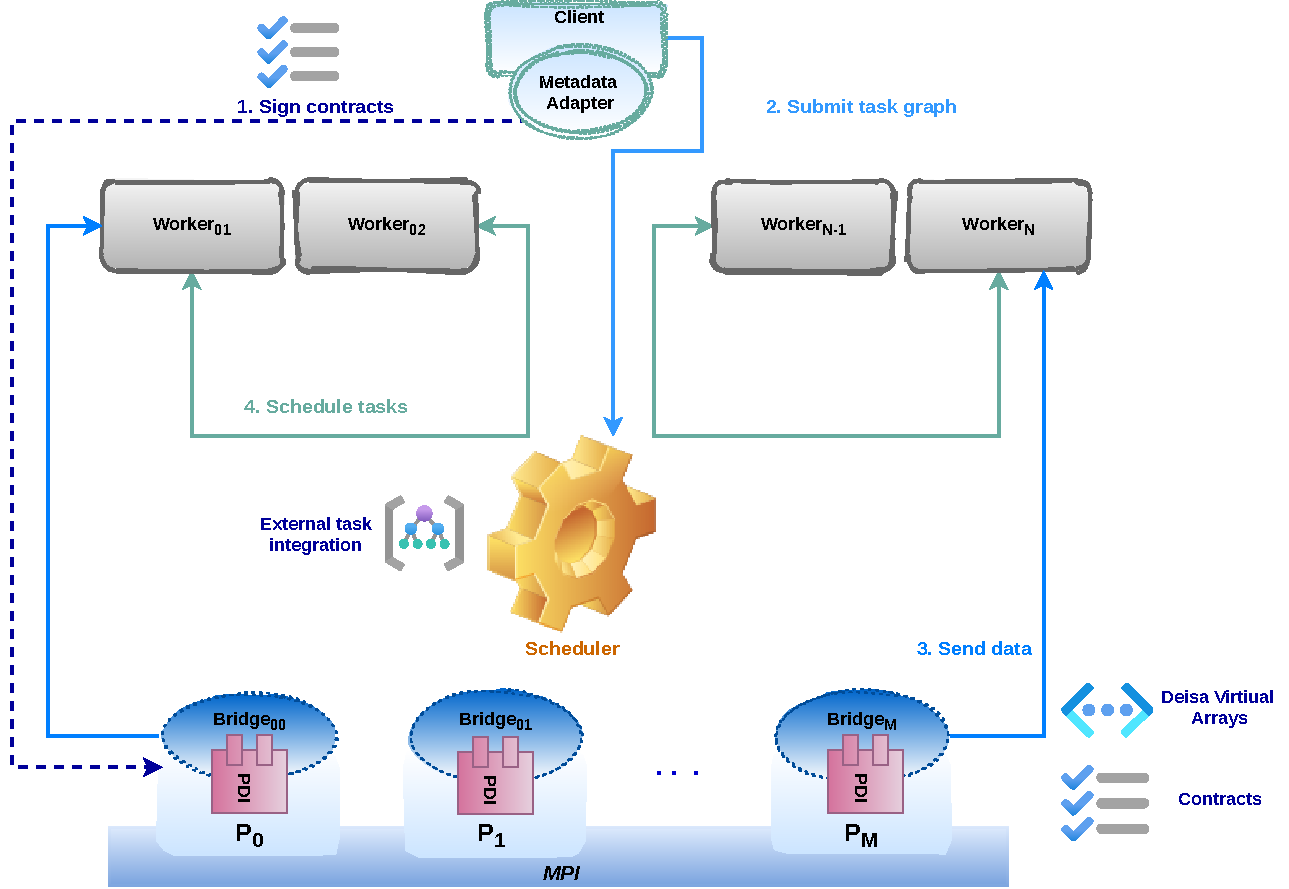
\includegraphics[width=\columnwidth]{figures/DeisaV2.pdf}
\caption{New \deisa architecture}
\label{figdeidav2}
\end{figure}

\section{Implementation}

We have implemented this version on top of \deisa. Most of the improvements are meant to achieve better performance and make \dask distributed support naively external tasks. To do so, we have extended the \texttt{scatter} function, introduced \texttt{external} tasks in a forked version of \dask distributed to support external tasks and improved the \deisa plugin to describe virtual arrays easily and support contracts. 

%One of the main limitations of \deisa that we wanted to address was the huge amount of metadata exchanged at each timestep and the amount of data which is sent to the workers even if it will not be needed. 

\subsection{Data Communication and Metadata management}

\subsubsection{Data Communication With Scatter}\label{sec:datacommscatter}

The \texttt{scatter} is a method in the \dask \texttt{Client} class. It is meant to send pieces of data from the client to the workers directly or by passing through the scheduler.

\begin{figure}\centering
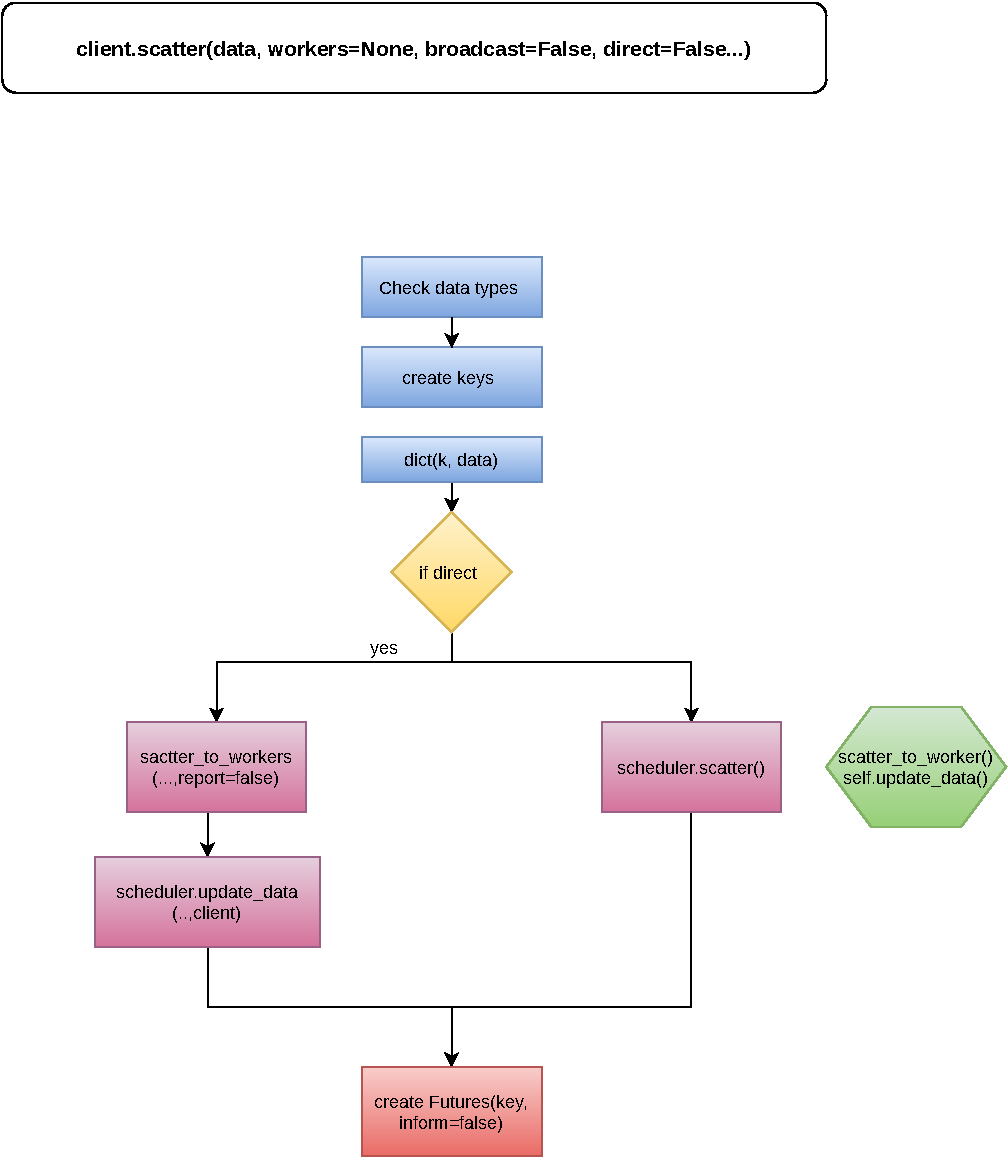
\includegraphics[scale=0.65]{figures/scatter.pdf}
\caption{Simplified pseudo-algorithm of the \dask implementation of \texttt{scatter} method}
\label{figoldscatter}
\end{figure}

Figure~\ref{figoldscatter} shows a simplified diagram of the pseudo-algorithm of the \texttt{scatter} method. The keys are created and associated with the data in a dictionary format. If the \texttt{Direct} option is activated, then the data is sent directly to the worker, which is relevant when large data is sent. If this option is not enabled then, the data is sent first to the scheduler and then to the workers via \texttt{scatter\_to\_worker} function. In the case of direct communication, the \texttt{scatter\_to\_worker} function does not inform the scheduler that the current client desires this data. This is done by calling the \texttt{scheduler.update\_data} that ensures relating the data identified by its key to the client that called the \texttt{scatter}. Once this is done, a \texttt{Future} object with the \texttt{finished} state is created. 

Note that the \texttt{scatter} is a complex process that involves the three entities in \dask distributed, namely the client, the scheduler and the worker. The \texttt{scatter\_to\_worker} function trigger a remote procedure call that calls the \texttt{worker.update\_data} function that updates the internal data of a worker without informing the scheduler.

If the worker informs the scheduler that new data is available in its memory, but this data is not associated with any client in the scheduler's data structures, then it will be deleted by the garbage collector. 
To prevent this scenario from happening, the worker only updates its internal data structures to keep track of the data in its memory but does not inform the scheduler.
The client from its side initiates a new RPC to the scheduler to call \texttt{scheduler.update\_data}, which will populate the internal data structures of the scheduler with the new data keys, associates them with the workers where they live (\texttt{who\_has} mapping) and the client who wants them (\texttt{wants\_what} mapping). This way, the data will not be deleted because there is at least one client that desires it.

Finally, once this is done, a local \texttt{Future} is created with the same \texttt{key}, and returned to the client in the \texttt{"finished"} status. 
Understanding the operation of the \texttt{scatter} and all the underlying functions was a very important step towards supporting in situ analytics in \dask. 

\subsubsection{\deisa Key Management System}
Unlike the synchronous version where the \texttt{dask.array}s are built on chunks whose keys are generated by \dask itself (that are returned by the \texttt{scatter} function). In this version, we have created and used specific keys to identify our data while keeping their semantics. 

Each key contains three main sections:  the prefix \texttt{deisa}, the name of the data, and the position of the chunk is the global array considering both time and space decomposition. For example, in  \texttt{(deisa-temp, (1,3,5))}, \texttt{temp} is the name of the data, $(1,3,5)$ is its position in the global array. This naming scheme can be extended to support multiple simulations as producers of data, feeding the same \dask cluster, by adding an identifier for the simulation, for instance. 

To avoid exchanging metadata between the two components at each timestep, and still be able to identify correctly the data generated by the simulation in the \dask component, we have set up a protocol with minimum communications. We use the same domain decomposition in both components by sending to \dask all needed information for that namely: the name of the generated array, its sizes and sub-sizes in all dimensions. On the \dask side, one key per block is created, associated with an array having the corresponding sizes, and identified as already explained. From the BSP component side, every time a process has to send a block of data, it will create a key using the same identification scheme. The only requirement is that each process should know the position of the block it generates; it may be its rank or any other expression.  


\subsubsection{\deisa Virtual Arrays}\label{sec:deisavirtualarr}

A \deisa virtual array describes the spatiotemporal domain decomposition of a generated data array. It contains the global sizes in each dimension, including the time dimension, the size of each block (size of generated data by each MPI process), and the starting indexes of each block. Describing the data in this way allows us to have a global view of the generated data. \deisa virtual arrays are used to create the \texttt{dask.arrays} in the analytics client, based on the \textit{external} tasks concept.

A \texttt{dask.array} that is created from a \deisa array descriptor contains only external data. We create a \texttt{"deisa"} task per MPI block per timestep. Technically, this is achieved by creating, in \deisa mode, a \textit{Future} with a specific key, per MPI block per timestep, and using the \textit{Future} to create a \texttt{dask.array}, then gathering all of the arrays to create a global \texttt{dask.array}. The chunking of this last corresponds to the spatiotemporal domain decomposition of the \deisa array. 

Figure~\ref{figdeisarray} shows an example of a \deisa virtual array construction, where we consider 2 main dimensions: space and time. Each MPI process generates a block per timestep, which is translated to a \deisa task and an external task too. 

The \deisa virtual arrays have been added to the configuration file of the \deisa plugin. Listing~\ref{ymldata} shows an example of a configuration file of the \deisa plugin. In line~\ref{ymldata:deisaarra} starts the list of the \deisa virtual arrays. For instance, here we have only the \texttt{Gtemp} array that is constructed of blocks of the \texttt{temp} data.

\begin{figure}\centering
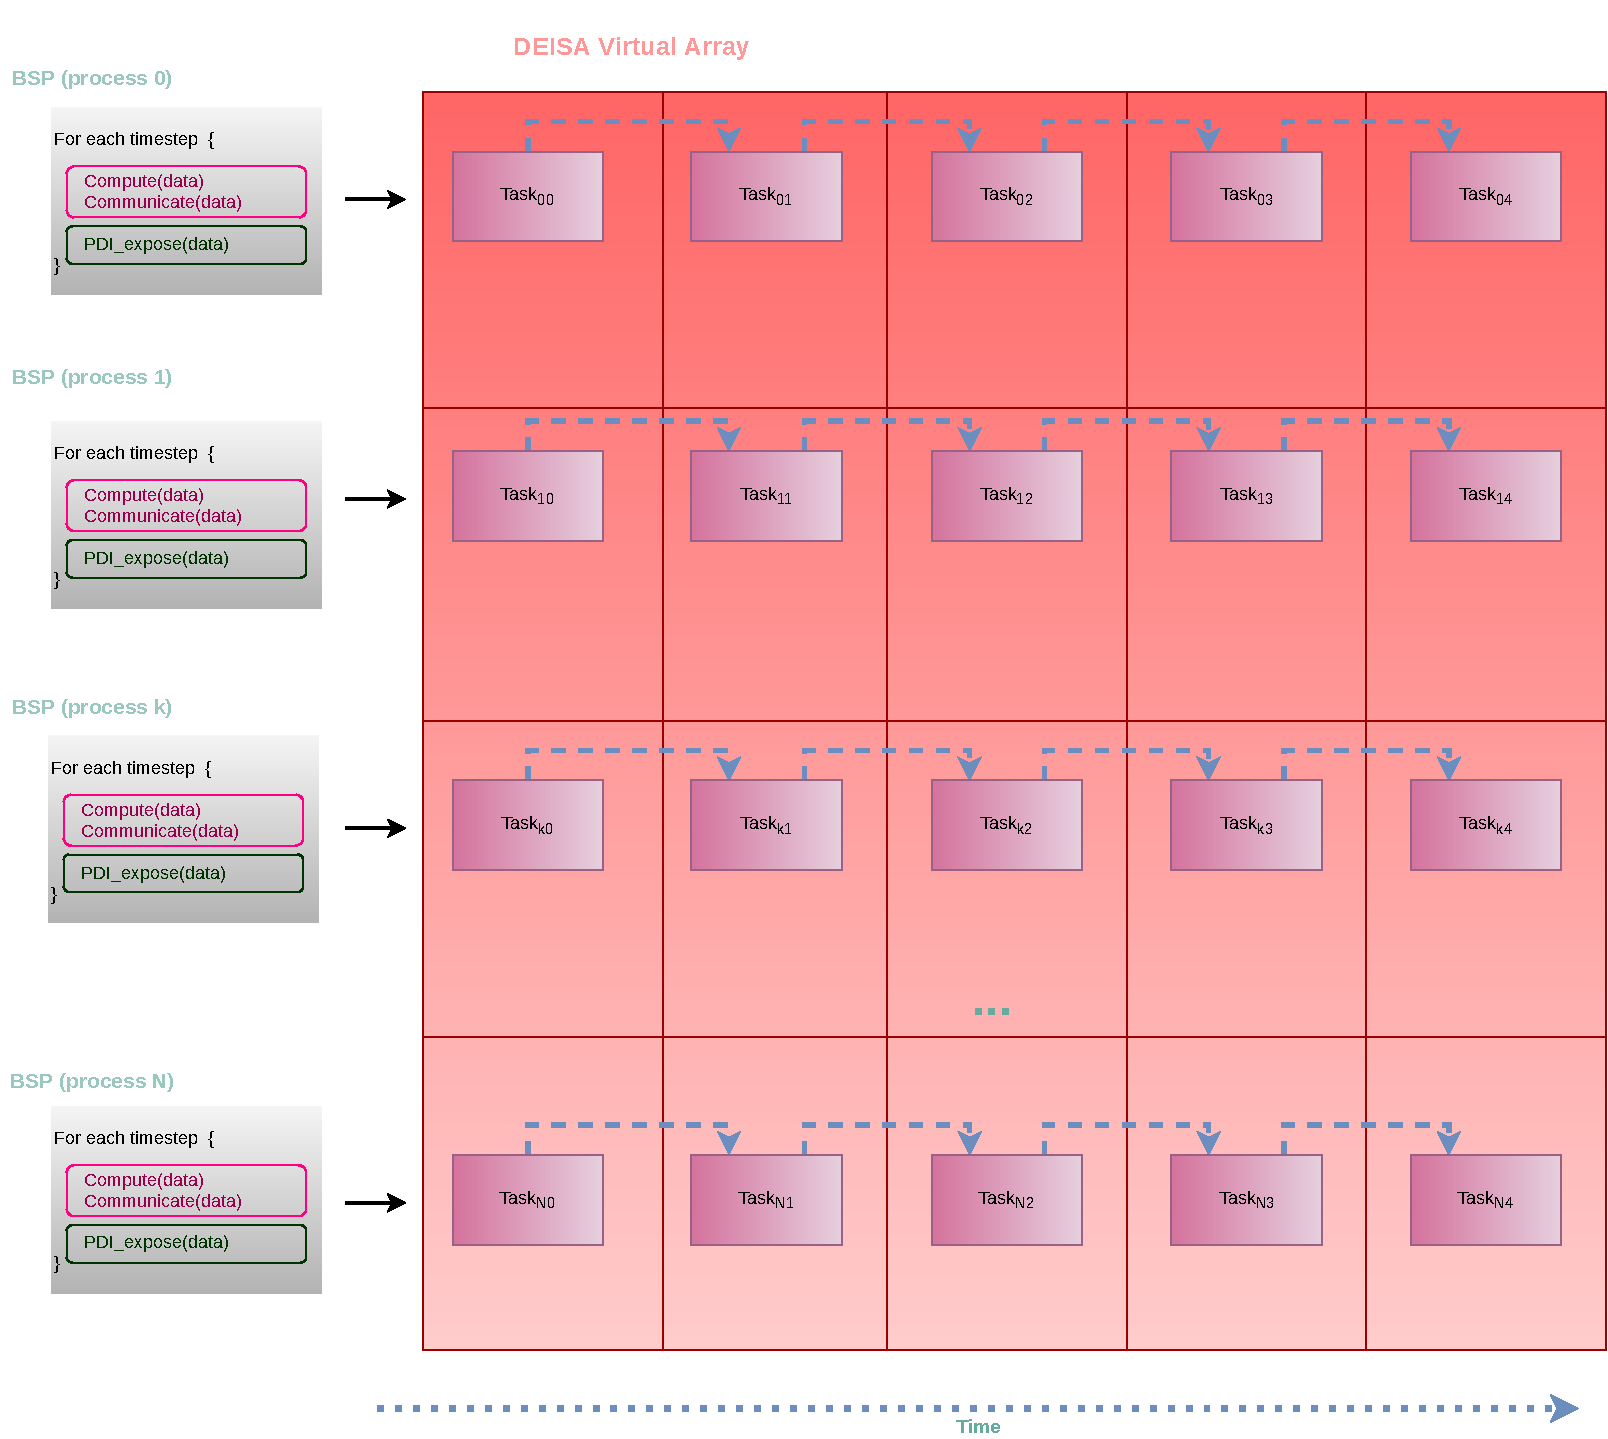
\includegraphics[scale=0.5]{figures/DeisaVirtualArrays.pdf}
\caption{\deisa virtual arrays structure}
\label{figdeisarray}
\end{figure}

\begin{lstlisting}[float, label=ymldata, language=yaml, caption=Data description in \pdi \deisa YAML file]
pdi:
    types: #[...] including config_t description
    metadata: {step: int, cfg: config_t, rank: int} |\label{ymldata:metadata}|
    data: |\label{ymldata:data}|
        temp: # the main temperature field |\label{ymldata:temp}|
            type: array |\label{ymldata:temp.type}|
            subtype: double |\label{ymldata:temp.subtype}|
            size: [ '$cfg.loc[0]', '$cfg.loc[1]' ]  |\label{ymldata:temp.size}|
    plugins:
        mpi: # get MPI rand and size
        deisa:
            scheduler_info: scheduler.json
            init_on: init 
            time_step: $step 
            deisa_arrays: # Deisa Virtual arrays |\label{ymldata:deisaarra}|
                G_temp: # Field name
                    type: array
                    subtype: double
                    size:
                        -'$cfg.maxTimeStep'
                        -'$cfg.loc[0] * ($rank % $cfg.proc[0])'
                        -'$cfg.loc[1] * ($rank / $cfg.proc[0])'
                    subsize: # Chunk size
                        -1
                        -'$cfg.loc[0]'
                        -'$cfg.loc[1]'
                    start:  # Chunk start
                        -$step
                        -'$cfg.loc[0] * ($rank % $cfg.proc[0])'
                        -'$cfg.loc[1] * ($rank / $cfg.proc[0])'
                    +timedim: 0 # A tag for the time dimension
            map_in: # Deisa array mapping
                temp: G_temp    
\end{lstlisting}


\subsubsection{Contracts}\label{sec:contracts}
%reecrire
As there is no automatic way to know if tasks depending on a given timestep are all processed or not, we have opted for the possibility of reducing the quantity of data sent at each timestep. We let the user manage the size of the memory needed by each worker and the number of workers depending on the time spent by the simulation in each timestep and the time spent by \dask to process the equivalent amount of data. To select only needed data, we have implemented contracts.

A contract is concluded between the simulation and \dask at the beginning of the simulation: The bridge in MPI process $0$ builds the \deisa virtual arrays descriptors using data from the simulation and sends them to the adaptor in \dask. The analytics client in \dask, gets access to the equivalent \texttt{dask.array}, and selects the data it is interested in from the available arrays, and sends back a selection request to the simulation bridge identifying the data it is actually interested in.

The contracts in the simulation side are checked every time data is available in an MPI process; if this block is included in the selection needed by the analytics, then the associated \textit{key} is created, and the data (identified by this created \textit{key}) is sent to a pre-selected worker. In the \dask side, the contracts are used at the beginning to create the corresponding \textit{dask.array}s to the \deisa virtual arrays. Similarly, \textit{keys} are created the same way in the adaptor. Those \textit{keys} are used to identify the chunks of the \texttt{dask.array} associated with that data. This way, only the description of the arrays sent in the contract process is performed; no need to send more metadata at each timestep. The contact process is summarized in Figure~\ref{figcontracts}.

\begin{figure}\centering
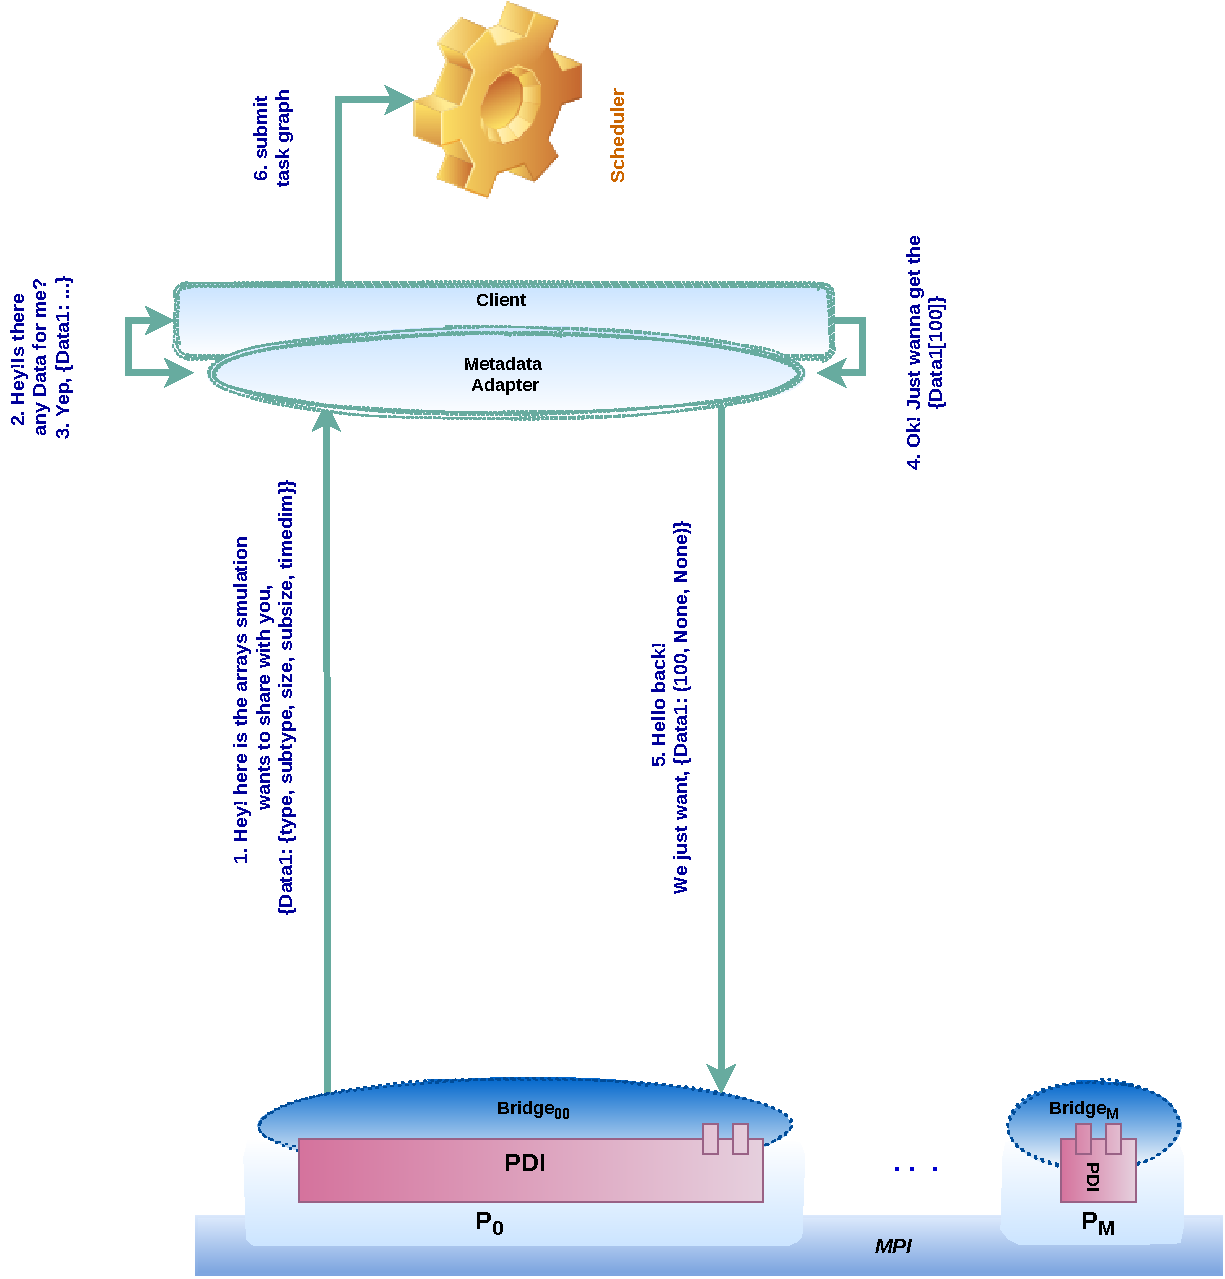
\includegraphics[scale=0.65,  angle=-90]{figures/Contracts .pdf}
\caption{The Contracts operation}
\label{figcontracts}
\end{figure}



\subsection{External Task and Asynchronous Scheduling}
\subsubsection{External Tasks in \dask Distributed}\label{sec:externaltasks}

\dask offers low and high-level libraries to create and submit tasks to the scheduler. The created tasks must be known and correctly defined to be used by \dask (see Section~\ref{sec:task} for more details about tasks in \dask distributed). Except for pure data tasks, a task has to include a callable (the function that the worker will execute). In this work, we want to use \dask for in situ analytics, so we suppose that the data is generated in another application, a running MPI simulation in this case, and we want to use that data as input to a \dask task graph. 

We define an \textit{external} task as work executed outside of the \dask cluster that generates data that will be used by \dask for analytics.  
We call those tasks \textit{external} tasks because they are run in an external environment rather than in \dask cluster. from the \dask point of view, those tasks can be seen as pure data tasks because the only known information about them is their output data.  

We have opted to explore the pure data task concept (via \texttt{scatter}) to integrate external tasks in \dask graphs. However, using by using it, we can only submit computations to \dask when data is sent to \dask via a \texttt{scatter}, and that's the way we have done that in the previous version of \deisa. 
Here we push this solution further to make \dask natively support external tasks, which makes us able to submit graphs on those external pure data tasks in advance (before data is available in the workers' memory). 

To do so, we have extended the \dask distributed core's task states with the new \textit{external} task concept. We have added a new task state called \texttt{"deisa"}. The task in a \texttt{"deisa"} state is identified by a unique key, and it is not schedulable nor runnable by \dask. 
Figure~\ref{figdasktaskstate} shows the newly added \texttt{"deisa"} state and the two main corresponding transitions: to \texttt{"memory"} when the data with the same key is now available in a worker's memory or to \texttt{"released"} when it needs to be deleted. 

\begin{figure}[tb]\centering
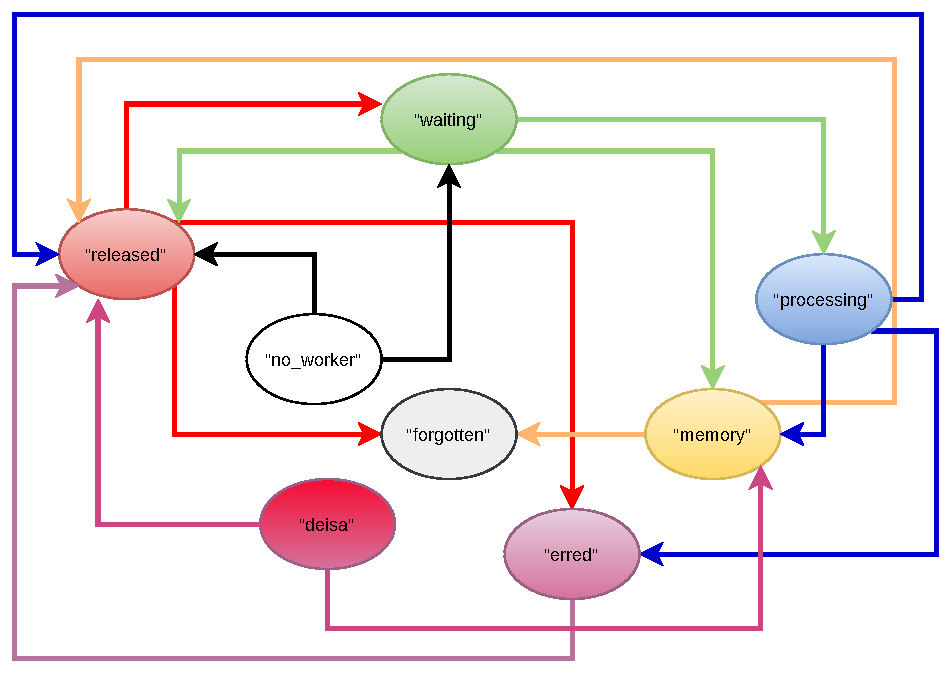
\includegraphics[scale=0.8]{figures/Dask-TaskStatesSheduler.pdf}
\caption{\dask task states and transitions}
\label{figdasktaskstate}
\end{figure}

The implementation of external tasks in \dask distributed extended mainly the client and the scheduler classes. The \texttt{Future} class in the client can be seen as a mirror of the tasks in the scheduler. In other words, the \textit{Future} is an interface that can be used by the client to check the state of the task in \dask scheduler and can retrieve their results as well. Figure~\ref{figfuturestate} shows \texttt{FutureStates} in the client and the corresponding \texttt{TaskStates} in the scheduler. In short, a \texttt{pending} \textit{Future} may be a task in one of these states {\texttt{"released", "retry", "waiting", "processing", "no-worker", "deisa"}}, and so on.  Thus to create an external task (a task in a \textit{"deisa"} state), we need to create a \texttt{Future} by specifying a unique \textit{key} and activating the \deisa mode by setting the \texttt{"deisa"} argument to \textit{True}. This will trigger an RPC to the scheduler to create a \texttt{"deisa"} task. 

\begin{figure}\centering
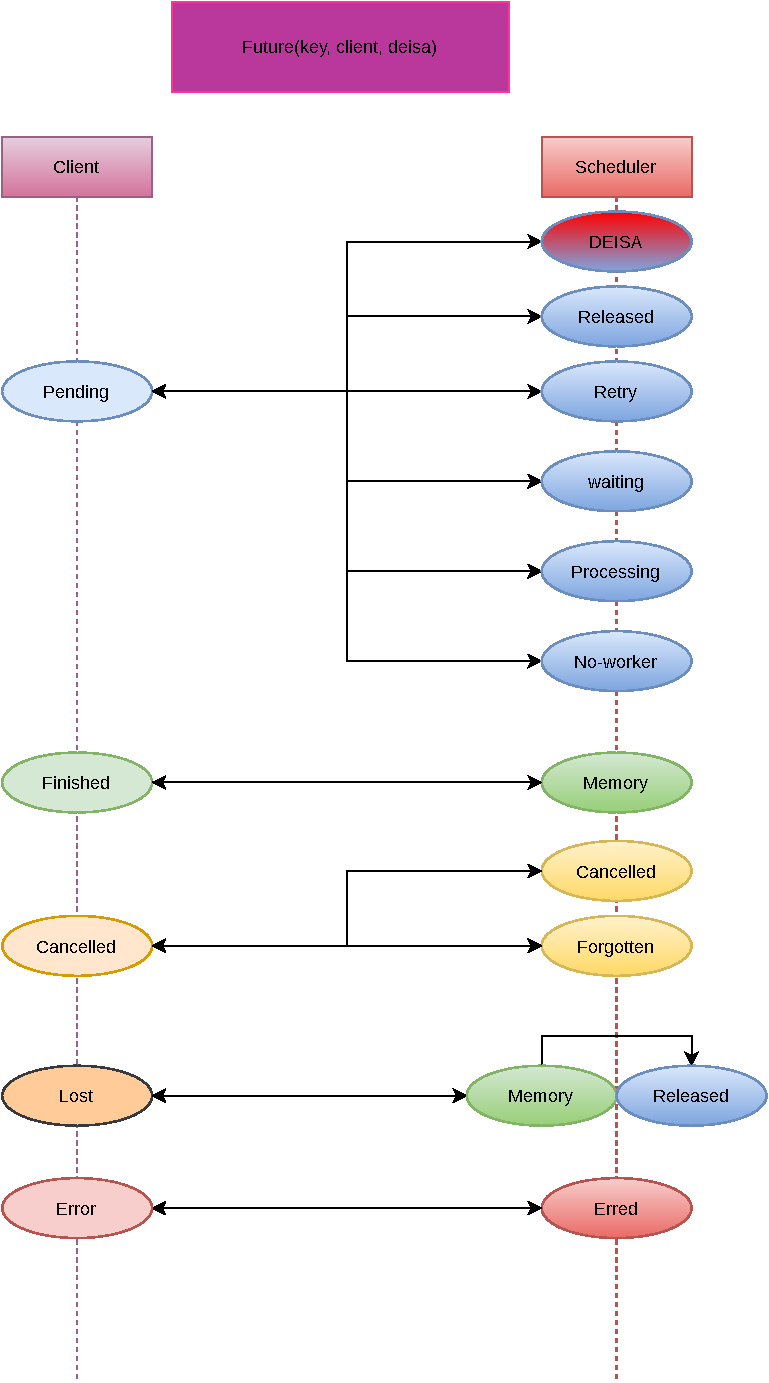
\includegraphics[scale=0.65]{figures/FutureStateClient.pdf}
\caption{Futures states and corresponding task states in the scheduler}
\label{figfuturestate}
\end{figure}

Figure~\ref{figscatterStates} shows a typical example of the task state transition of an external task. We consider in this figure one bridge that represents the external application, a \dask scheduler, a client and a worker.
In this figure, we do not represent all RPC between the different components. Our goal is to show that we are representing the exact same task in different places. We identify it by its unique key: \texttt{key1}. First, we create a \textit{Future} in the client, which is identified by \texttt{key1} and enabling \deisa mode, the creation of the \textit{Future} triggers the creation of a task in the \texttt{"deisa"} state in the scheduler. At some point, the data that is identified by the same \texttt{key1} is sent to worker1, so the state of this date becomes \texttt{"memory"} in worker1, then the \texttt{"deisa"} task in the scheduler switches to the \texttt{"memory"} state as well. Once this is updated in the scheduler, all clients and bridges desiring the \texttt{key1} are informed that the task is finished, and thus the \textit{Future} switches to \textit{finished} state. 

The magic behind this example will be explained in the next section, with all the remote procedure calls. Here the goal is to show the correspondence between a task in the scheduler, a pure data task in the worker and the \texttt{Future} on the client side. 

\begin{figure}\centering
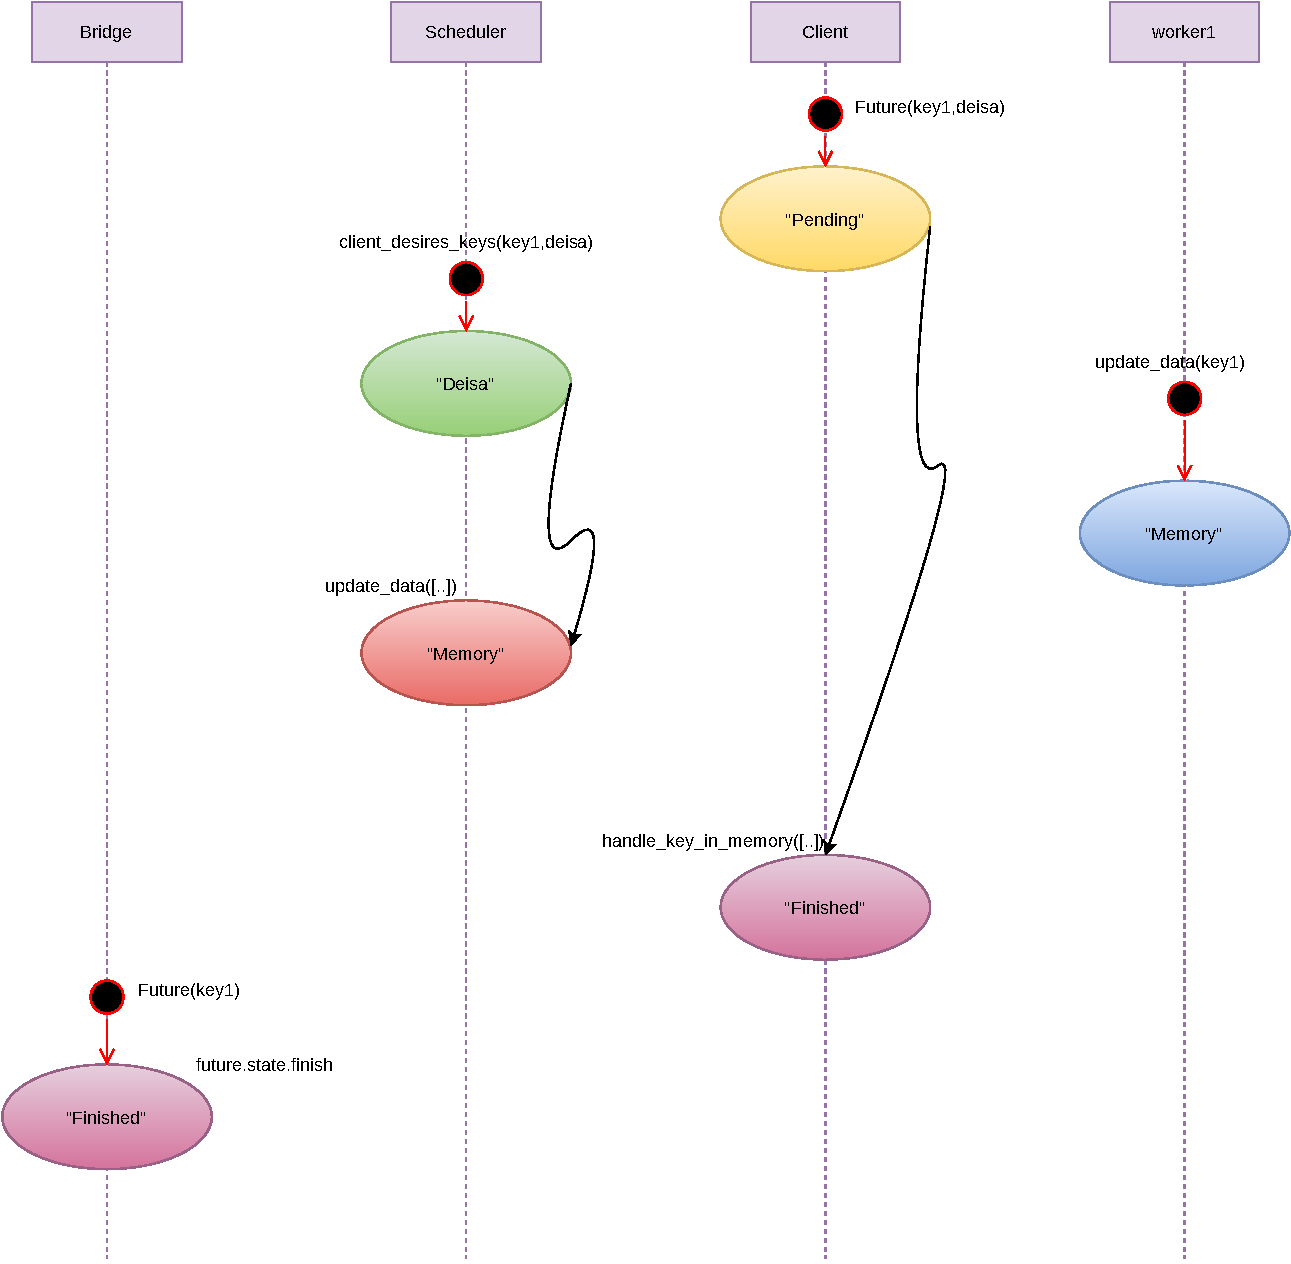
\includegraphics[scale=0.65]{figures/NewSacatterAutomateexample.pdf}
\caption{External task state scenario diagram}
\label{figscatterStates}
\end{figure}


\subsubsection{Asynchronous Scheduling of External Task in \dask}\label{sec:asynchscheduling}

The goal of updating the default scatter system is to make \dask distributed support asynchronous scheduling. In other words, submit a task graph to \dask, that contains \textit{external} tasks. 

\begin{figure}\centering
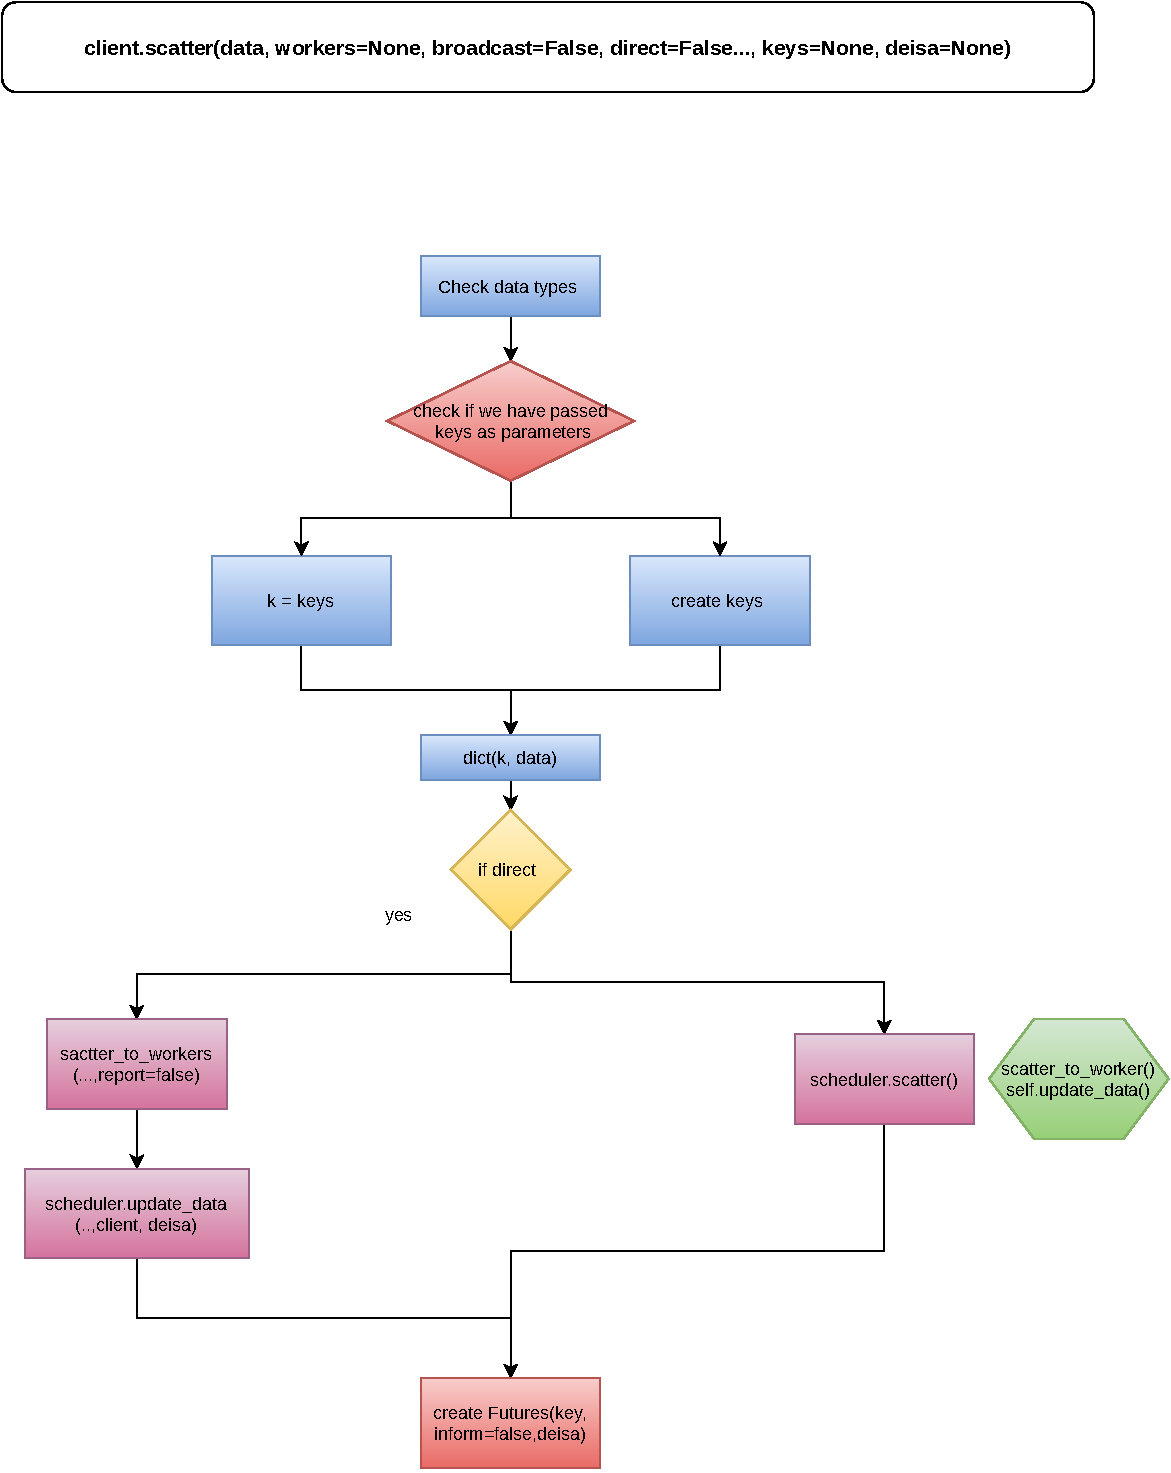
\includegraphics[scale=0.65]{figures/Dask-scatter().pdf}
\caption{New \texttt{scatter} pseudo-algorithm diagram}
\label{figscatter}
\end{figure}

Figure~\ref{figscatter} represents the updated version of \texttt{scatter} in the frame of supporting in situ analytics. We have added two main parameters to the method: \texttt{keys}, and \texttt{deisa}, both of them are \texttt{None} by default. \texttt{keys} is a list of keys associated with a list of data we want to communicate. In our case, it is always a list of one element. and \texttt{deisa} is an argument that is forwarded to the \texttt{scheduler.update\_data} and \texttt{Future.\_\_init\_\_}  methods  that changes the default operation when \texttt{deisa} mode is activated.

The \texttt{Future.\_\_init\_\_} with \texttt{deisa} mode here does not matter because the status of the \textit{Future} is turned to a \texttt{'finished'} status before the client returns from the \texttt{scatter}.
What really matters is the \texttt{scheduler.update\_data} method that needed to be changed. To understand the need for the made modifications in this method, we have to explain two main points.

First, let's recall how \dask scheduler manages finished tasks. When data is an output of a finished task in \dask, the worker sends a message to the scheduler, including, among other information, the key of the task and \textit{"task-finished"} stimulus. Depending on the stimulus, the scheduler triggers different handlers, and in this particular case, it is the \texttt{handle\_task\_finished} which is called. 
This handler triggers the transition process(see Section~\ref{sec:scheduling}), which unblocks the dependent tasks, and the scheduling keeps going.

Now let's go back to the \texttt{scatter}. It has been introduced in \dask to send external data to the cluster. So by definition, this data does not exist in \dask, and it is not even known before it is sent. The associated \texttt{key} with this data is created in the \texttt{scatter} function itself (as shown in the diagram in Figure~\ref{figscatter}), so this data can only be used in a task graph after the \texttt{scatter} is finished and returned.
The way the scheduler manages the data it gets from a \texttt{scatter} is quite different from the way it manages data issued from an ordinary computed task by a worker, even if both of them are considered as tasks in the \texttt{"memory"} state.

As shown in the diagram in Figure~\ref{figscatter}, to inform the scheduler about this new data, the method \texttt{scheduler.update\_data} is called. The left part in Figure~\ref{figsceculerupdatedata} shows a simplified pseudo-algorithm of the \texttt{scheduler.update\_data}; mainly, only the scheduler's internal data structures are updated. So there is no transition process done in \texttt{scheduler.update\_data}. This is a normal operation because we suppose that the data is not known before it is sent to \dask workers. 

\begin{figure}\centering
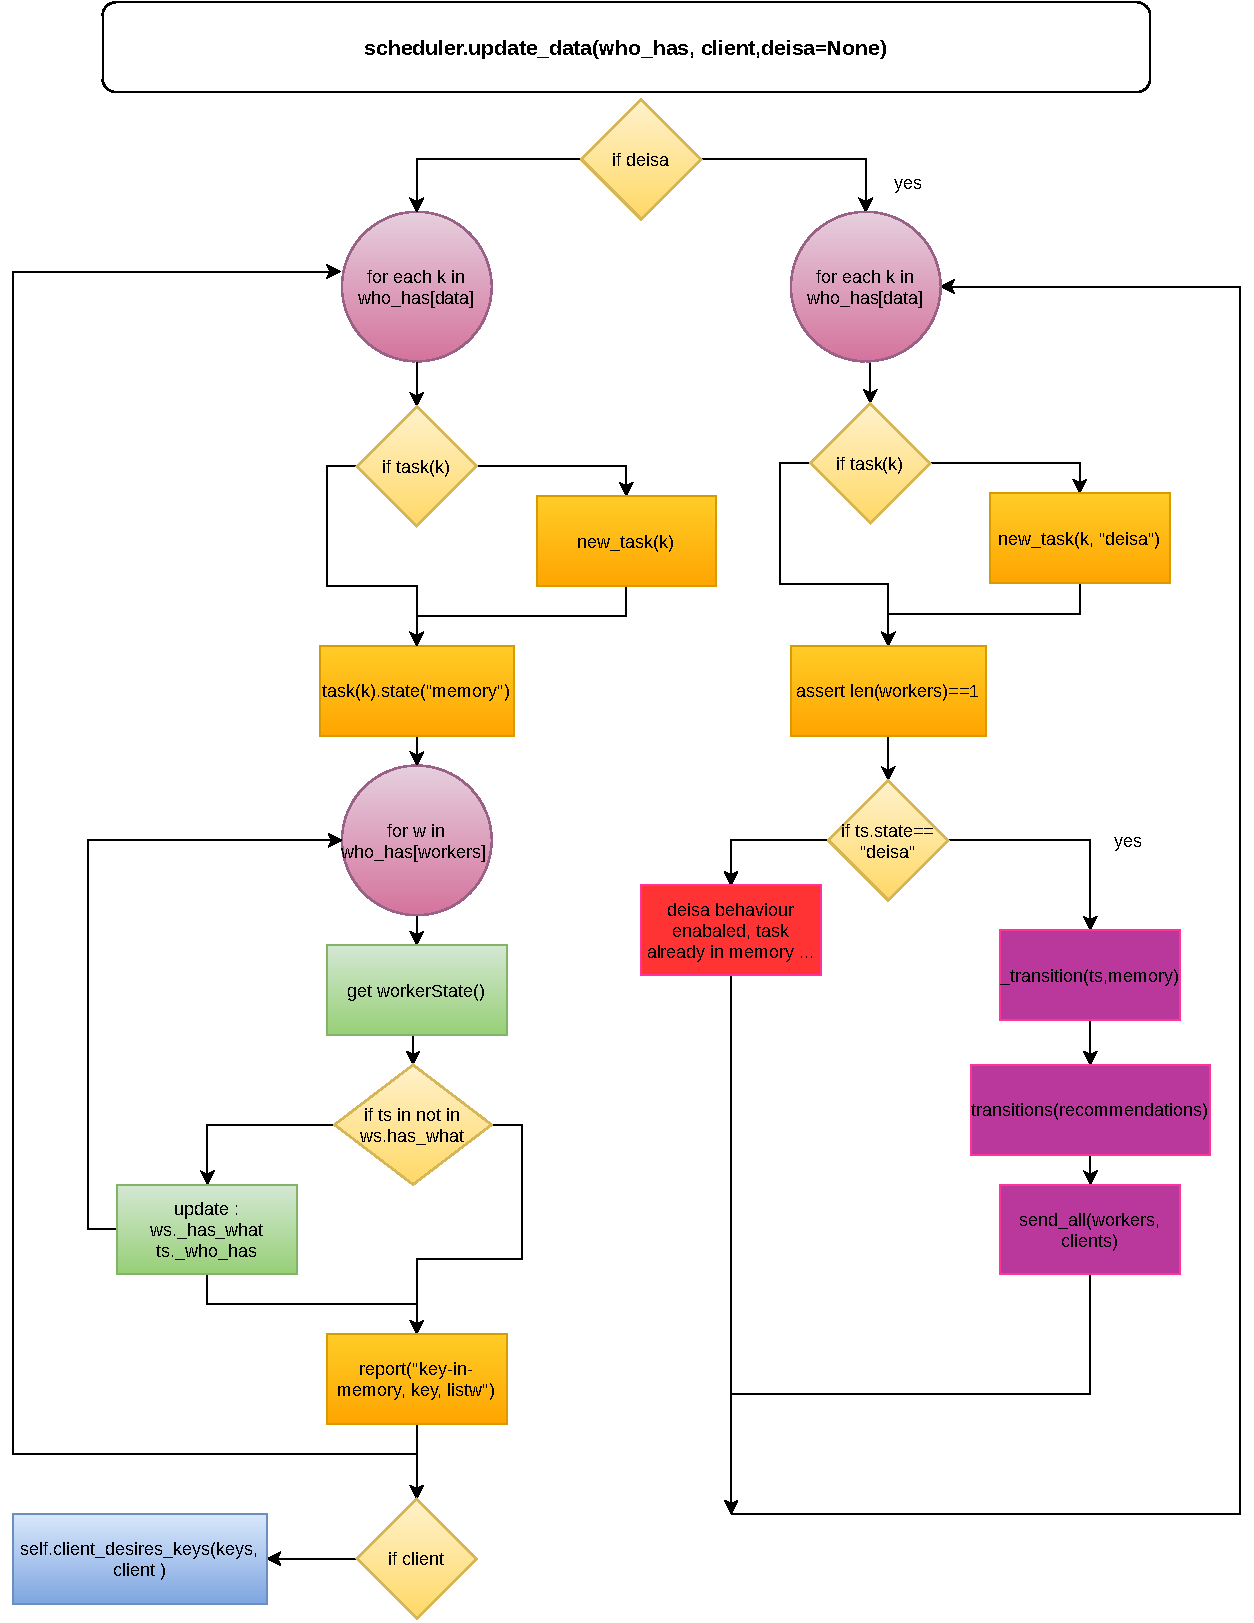
\includegraphics[scale=0.65]{figures/scheduler_update_data().pdf}
\caption{Scheduler update\_data method}
\label{figsceculerupdatedata}
\end{figure}

To be able to make \dask natively support external tasks, we have to make it treat them as any other finished task. This means that \dask will not only update its internal data structures, but it will also trigger the transition process to unblock the depending tasks.  And that is mainly what has been done in the right part of Figure~\ref{figsceculerupdatedata}. When \deisa mode is activated, we update the scheduler's internal data structures and trigger the transition process: starting by transiting the current task to \texttt{"memory"} state, then making all underlying transitions.    


\subsubsection{Full External Task scenario}

Now that we have explained how to support the external task in \dask, here is a complete example (Figure~\ref{figscatterDA}) that shows and explains the magic behind the example in Section~\ref{sec:externaltasks}. 

\begin{figure}\centering
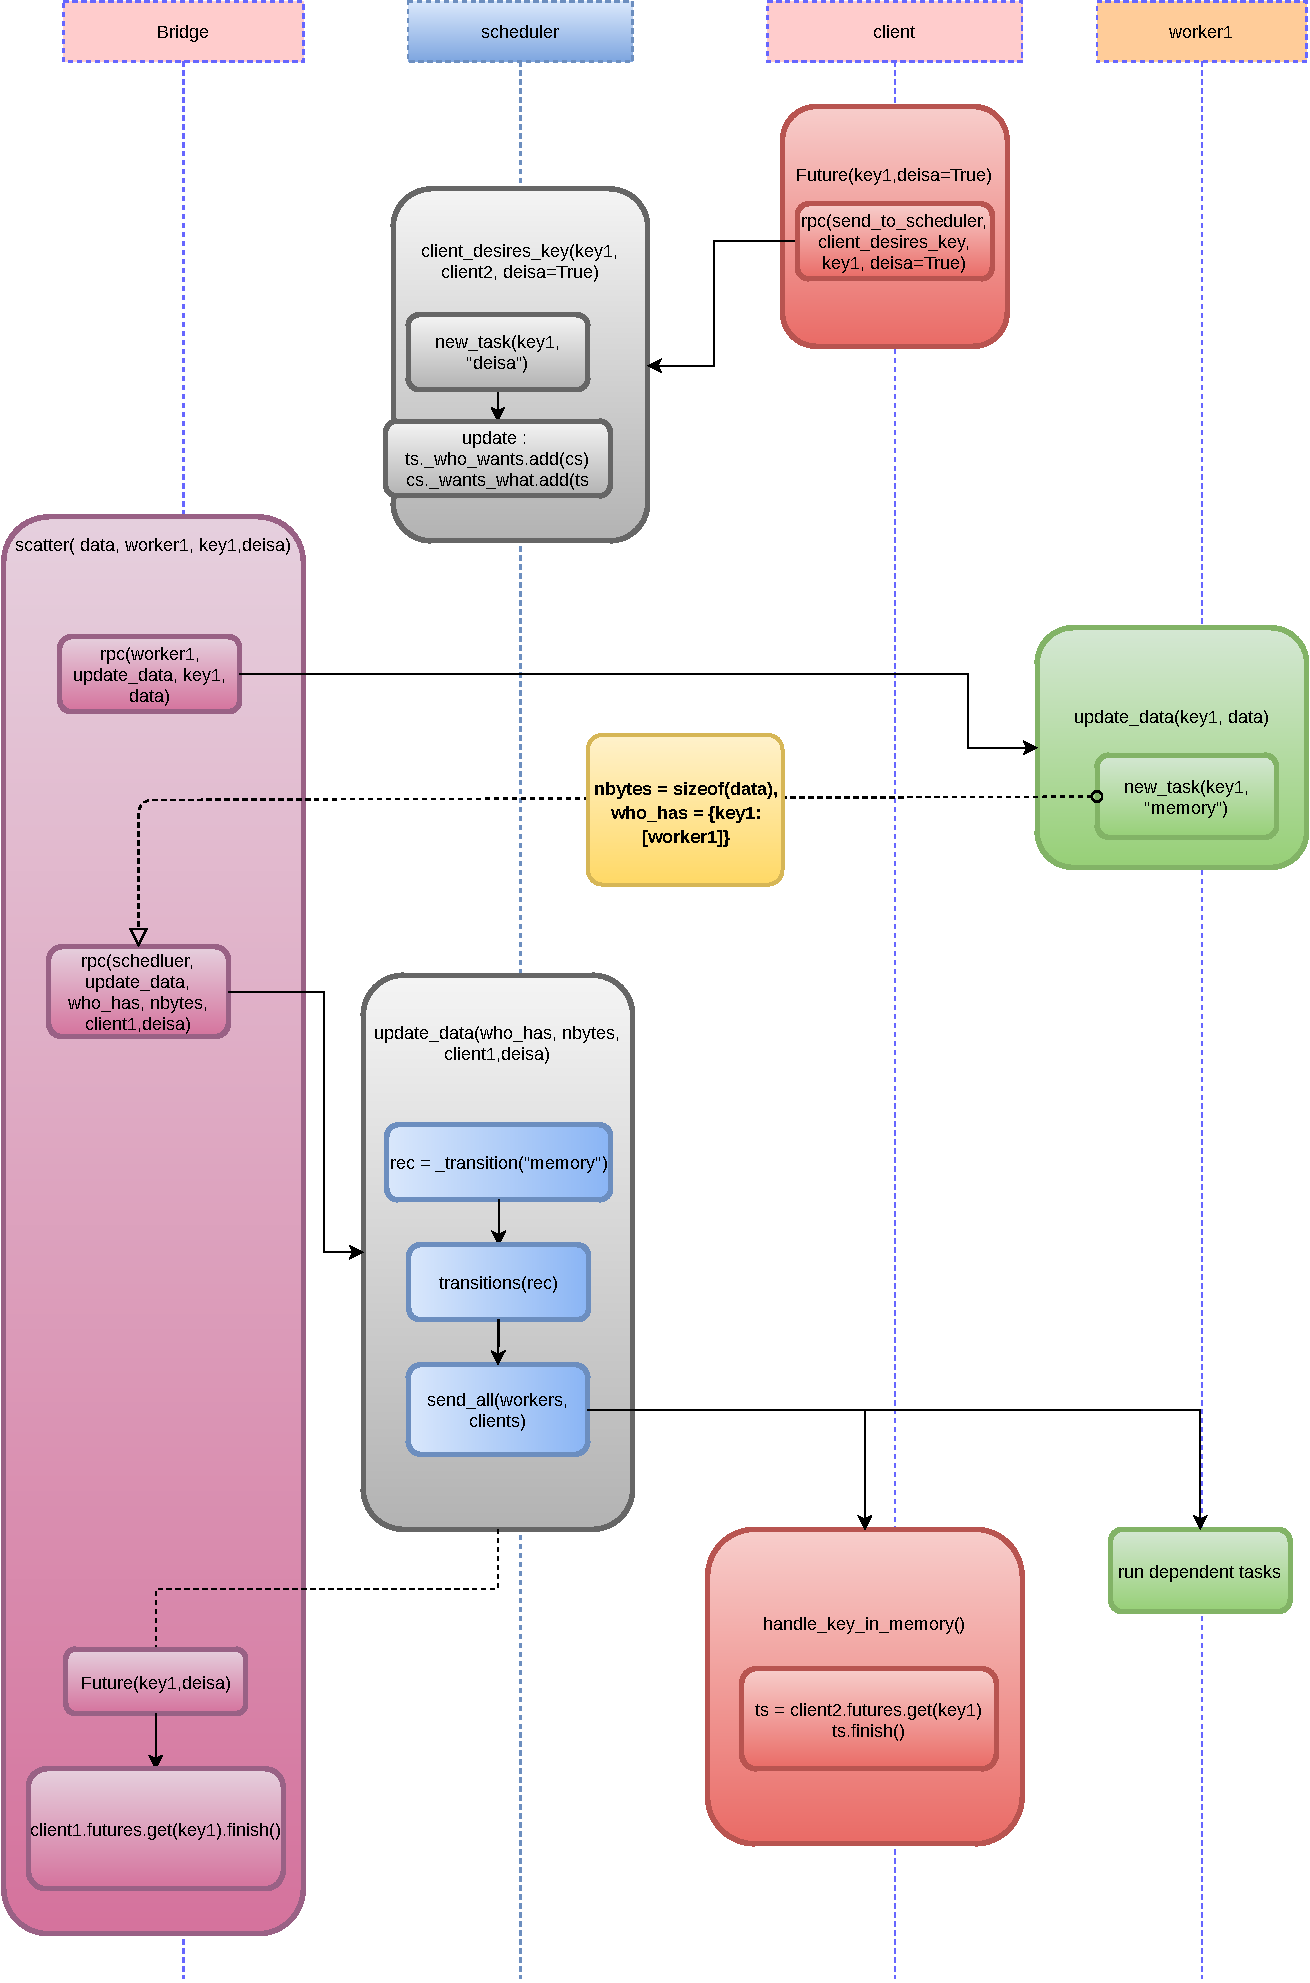
\includegraphics[scale=0.65]{figures/NewScatterDiagramAtcivity.pdf}
\caption{Activity diagram of a typical external tasks scenario}
\label{figscatterDA}
\end{figure}

In this diagram, there are two independent sequences. We suppose here that the top sequence is executed first, so we have only drawn methods called in that scenario. However, if the second sequence is launched first, then this workflow works but in a different scenario. 

When the client creates the \textit{Future} with \texttt{key1} and \texttt{deisa=True} as arguments, an RPC is done: the client sends a message to the scheduler saying that it desires the results of the task \texttt{key1} (or the data \texttt{key1} if it is a pure data task). The scheduler handles this message internally, creates a task in the \texttt{"deisa"} state because \deisa mode was enabled, and updates its internal data structures. 

The second part of the diagram starts when the bridge calls the modified \texttt{scatter} method, with \deisa mode activated and using the same key: \texttt{key1} and specifying the worker \texttt{worker1}. The bridge calls \texttt{worker.update\_data} (using the same key). This call makes the worker update its internal data and internal data structure to make \texttt{key1} to the \texttt{"memory"} in the worker1. Then returns some metadata to the bridge regarding the size and mapping of the \texttt{key1} to the \textit{worker1}.

Once this is received in the bridge, it triggers an RPC again, and this time to the scheduler to update its data with the information it got from the worker and by activating the \textbf{\deisa mode}. Now that the \texttt{scheduler.update\_data} is modified to support external tasks, the scheduler updates its internal data structures and starts the transition process. At the end of this process, it sends messages to concerned clients and workers. For the client and the bridge, they are informed that the \texttt{key1} is now in memory, so they turn their \textit{Future}s to the \texttt{"finished"} status, and the worker1 will likely run dependent tasks on \texttt{key1}.


\subsection{User API and Configuration}

\subsubsection{\deisa Plugin Configuration}

We implemented a \deisa plugin to support the new functionalities. The plugin responds to both data sharing and \pdi events. The specification tree of the plugin contains 5 main keywords:

\begin{itemize}
    \item \texttt{scheduler\_info}: takes a string that represents the path to the \texttt{json} scheduler file that contains connection information. When the scheduler is launched, it generates this file with the name passed to the option \texttt{--scheduler-file}. 

    \item An \texttt{init\_on} initialization event to gather all the needed metadata data and send them to the \deisa adaptor. The needed metadata have to be shared by the simulation before the \texttt{init\_on} event is issued. At the \texttt{init\_on} event, the contracts are signed between the simulation and \dask. We detail the contract process in Section~\ref{sec:contracts}.
    
    \item The \textit{time\_step} variable that represents the iterator over the time dimension. It is needed to create the unique key to the associated data.  
    
    \item A \texttt{deisa\_arrays} section that describes the global data arrays following time and space distributions, independently from local data name; 
    
    \item a \texttt{map\_in} section maps local buffer's name (defined in the \texttt{data} section of \pdi) to the \texttt{deisa\_arrays}'s name. We detail the \deisa virtual array implementation and use in Section~\ref{sec:deisavirtualarr}. 
\end{itemize}


\subsubsection{User API}

The bridge's user API is now hidden with the new declarative interface of the specification tree of the \deisa plugin. The new interface is easier and hides all implementation details.

We have kept recalling until now that the main goal of this work is to bring post hoc easiness to the in situ environment. Thus the user API has to be as much as possible similar to the post hoc one or at least comparable. The user API in the new version of \deisa consists of four main functions: 
\begin{itemize}
    \item \texttt{Deisa(scheduler\_file, nbr\_workers)} returns a \deisa Adaptor object, the scheduler\_file is the file returned by the scheduler when it is launched(see Section~\ref{sec:launch}), and nbr\_workers is the number of workers that need to be connected.  

    \item \texttt{Adaptor.get\_client()} returns a \dask client, it can be used to submit analytics to the scheduler and use all available Client API in \dask distributed.
    
    \item \texttt{Adaptor.get\_deisa\_arrays()} returns a dictionary where the keys are strings representing the names of available data, and the values are \deisa arrays. The square brackets operator can be used to select a \deisa array, and a square brackets operator is also implemented to make a selection in the \deisa array to get a \texttt{dask.array}. If all the array is needed, the Ellipsis \texttt{...} can be used to select all the array.
    
    \item \texttt{Deisa\_arrays.validate\_contracts()} to validate the selection that we did and ask for that data. More details in contacts are explained in Section~\ref{sec:contracts}.
\end{itemize}


\begin{lstlisting}[float, label=listderiv, language=python, caption=In situ incremental temporal derivative]
from deisa import Deisa

# Derivative function
def Derivative(F, dt):
    """
    First Derivative
       Input: F        = function to be derivate
              dt       = step of the variable for derivative
       Output: dFdt = first derivative of F
    """
    c0 = 2. / 3.
    dFdt = c0 / dx * (F[3: - 1] - F[1: - 3] - (F[4:] - F[:- 4]) / 8.)
    return dFdt

# Scheduler file name and configuration file
scheduler_info = 'scheduler.json'

# Initialize Deisa
Deisa = Deisa(scheduler_info, nbr\_workers)

# Get client
client = Deisa.get_client()

# Get available deisa arrays 
arrays = Deisa.get_deisa_arrays()

# Select data: 1/2 timesteps
gt = arrays["global_t"][::2]

# Construct a lazy task graph
cpt = derivative(gt, 1)

# Submit the task graph to the scheduler
s = client.persist(cpt)

# Sign contract
arrays.validate_contract()

print(client.compute(s).result(), flush=True)
client.shutdown()
\end{lstlisting}


\section{Experiments and Evaluation}
In this section, we present the experiments we have performed to evaluate our new prototype. First, we present our experimental environment in the Irene supercomputer. Then talk about the software we have used in the experiments, namely a new version of the incremental PCA and a temporal derivative. We show our comparisons to the previous version of \deisa and the post hoc experiments. We will discuss those results and explain eventual similarities and differences between the different versions.  

\subsection{Environment Installation}
One of the good practices for HPC reproducibility is using the same environment over experiments. To ensure this, we have used spack to install our environment with all needed dependencies instead of relying on the available module systems in the supercomputers. 
In some supercomputers like Irene, users do not have access to the internet, so we had to pre-fetch needed packages in a machine with internet access, then create a mirror and send it to Irene using \texttt{rsync}. Once this is done, you can use the local mirror in the supercomputer to install the packages.  The configuration file in Listing~\ref{spack} shows an example of a configuration file to create a spack environment.     

\begin{lstlisting}[float, label=spack, language=yaml, caption=Spack environment installation configuration file]

spack:
  concretization: together
  specs:
  - netlib-lapack, pdi, pdiplugin-decl-hdf5, pdiplugin-deisa, py-dask+diagnostics py-h5py, pdiplugin-mpi, pdiplugin-pycall
  view: true
  packages:
    all:
      buildable: true
      permissions:
        write: group
        group: group001
      compiler:
      - gcc
      providers:
        mpi:
        - openmpi
    openmpi:
      buildable: false
      externals:
      - prefix: /ccc/products/openmpi-4.0.3/gcc--9.3.0/default/
        spec: openmpi@4.0.3%gcc@9.3.0+cuda+cxx~cxx_exceptions~java+lustre~memchecker+pmi+pmix~sqlite3~static~thread_multiple~wrapper-rpath
          fabrics=ucx schedulers=slurm
        modules: [gnu/9.0.3, openmpi/4.0.3]
  repos:
  - /path/to/spack/var/spack/repos/pdi
  mirrors:
    mirror-gysela-deisa:
      fetch:
        url: file:///path/to/mirror-gysela-deisa

\end{lstlisting}

We have also provided a spack recipe for the cloned version of \dask distributed that supports the external tasks in \dask, and a recipe for \deisa plugin that can be found on GitHub repository\footnote{https://github.com/pdidev/spack}. The \deisa python API can be installed through Pypi\footnote{https://pypi.org/project/deisa/}.  

\subsection{Software}
We have used the same simulation MiniApp to evaluate the new version of \deisa, and provided evaluation with two different analytics, an in situ version of the incremental PCA and a temporal derivative of the generated data.   

\subsubsection{In Situ Incremental PCA}\label{ISIPCA}

We have implemented a new version of the incremental PCA that takes a multidimensional array and computes its PCA incrementally. Thus it can be used for both post hoc and in situ. 
Moreover, we have provided a similar interface to the sequential PCA by hiding the incremental execution of the IPCA.

In addition to the multidimensional array, the \texttt{fit(ndarray, label\_list, feature\_labels, sample\_labels)} method takes three new parameters:
\begin{itemize}
    \item ndarray: array-like or sparse matrix that will be chunked to N chunks in the first dimension, where N is len(ndarray). We suppose that dimension zero is the time dimension.
    \item \texttt{label\_list}: a list of $N$ strings that represents the labels of the N dimensions of the ndarray. It will be used to create an \texttt{xarray}.
    \item \texttt{feature\_labels}: a list of $X$ strings, included in \texttt{label\_list}, that represent the dimensions we want to consider as features. They will be stacked into the features' dimension. 
    \item  \texttt{sample\_labels}: a list of $Y$ strings, included in \texttt{label\_list}, that represent the dimensions we want to consider as samples, where $X+Y=N$. They will be stacked into the samples' dimension.
\end{itemize}

We have used the \texttt{xarray} library to stack the features' dimensions together and the samples' dimensions together to get a 2D array at the end and use the incremental PCA over the time dimensions. The \texttt{fit\_transform(ndarray, label\_list, feature\_labels, sample\_labels)} method takes the same parameters.

\subsubsection{Incremental Time Derivative}

The derivative is very important in physics; it represents the rate of change and leads to precise modelling of the quantity under study. Computing the derivative in post hoc is memory-consuming because we need several timesteps at once to compute a derivative at a given timestep.
In this work, we are interested in the time derivative in particular because it demonstrates the variation over time. Since the simulations are discrete, to approximate the derivative, we use the finite difference\cite{fornberg_generation_1988}. 

Thanks to \textit{dask.array} API and the new version of \deisa, an incremental in situ time derivative, is a one-line stencil computation (see Listing~\ref{listderiv}). The user does not need to manage memory or the incremental nature of the algorithm. \dask launches the tasks when the data is available. 

\subsection{Performance Evaluation}
In this section, we evaluate the new version of \deisa compared to the previous prototype and post hoc analytics. We will use the new interface of the IPCA for both \deisa and post hoc analytics and show the importance of the contract through the incremental time derivative.
We have used the chunking in HDF5 to improve post hoc performance in those experiments.
In the different figures, the results for the previous \deisa prototype are referenced with DEISA1, 
the results for the new version of \deisa without contracts and a heartbeat interval set to 1 min with DEISA2, 
and the full new version with a $\infty$ heartbeat interval is DEISA3.

\begin{table}[ht]
\centering
\begin{tabular}{||c  c||}
\hline
 Parameter                         & Value \\
\hline\hline
Number of runs                      & 3   \\
Number of iterations IPCA           & 10  \\
Number of iteration Derivative      & 12  \\
 MPI nodes / \dask worker node      & 2   \\
 MPI process / MPI node             & 2   \\
 Dask worker / \dask worker node    & 2   \\
 Thread / \dask worker              & 24  \\
 MPI process / \dask worker         & 2   \\
\hline
\end{tabular}
\caption{\label{parameters3}Fixed parameters used in Experiment III~\ref{XP3} and~\ref{XP4}}
\end{table}


\begin{table}[ht]\centering
\begin{tabular}{||ccccc||}
\hline
 Configuration              & XP1:128\,MiB  & XP1:256\,MiB  & XP1:512\,MiB      & XP1:1\,GiB\\
\hline\hline
 MPI block size             & 128                 & 256                  & 512   & 1       \\
\dask chunk size            & 128                 & 256                  & 512   & 1       \\
\multicolumn{1}{||c}{MPI Nodes}                   &\multicolumn{4}{c||}{[4, 8, 16, 32, 64, 128, 256]} \\
\multicolumn{1}{||c}{\dask Nodes}                 &\multicolumn{4}{c||}{[2, 4, 8, 16, 32, 64, 128] }\\

\hline\hline
\end{tabular}
\caption{\label{config3}The three configurations of Experiment~\ref{XP3} and~\ref{XP4}}
\end{table}

We have performed two main experiments with the parameters and configuration in Table~\ref{parameters3} and Table~\ref{config3}:
\begin{itemize}
    \item \textbf{Experiment III} compares the performance of \deisa with and without contracts (DEISA3 vs DEISA2) and the old version (DEISA1)
    \item \textbf{Experiment IV} compares the new version of \deisa (DEISA3) performance to the old version (DEISA1) and to parallel post hoc analysis with plain \dask (DASK) using the old version of the Incremental PCA presented in Section~\ref{IPCA}, and using the newly developed version presented in Section~\ref{ISIPCA}. 
\end{itemize}

\subsubsection{Experiment III}\label{XP3}
Those experiments have been performed in the Irene supercomputer. We have used the developed MiniApp for the three implementations of \deisa. Table~\ref{parameters3}  and Table~\ref{config3} are the used parameters and configurations also in these experiments. In those experiments, we were just interested in the communication time. 
To show the importance of contracts, we have decided to keep one 1/2 iterations.
 
\begin{figure}
     \centering
     \begin{subfigure}[b]{0.4\textwidth}
         \centering
         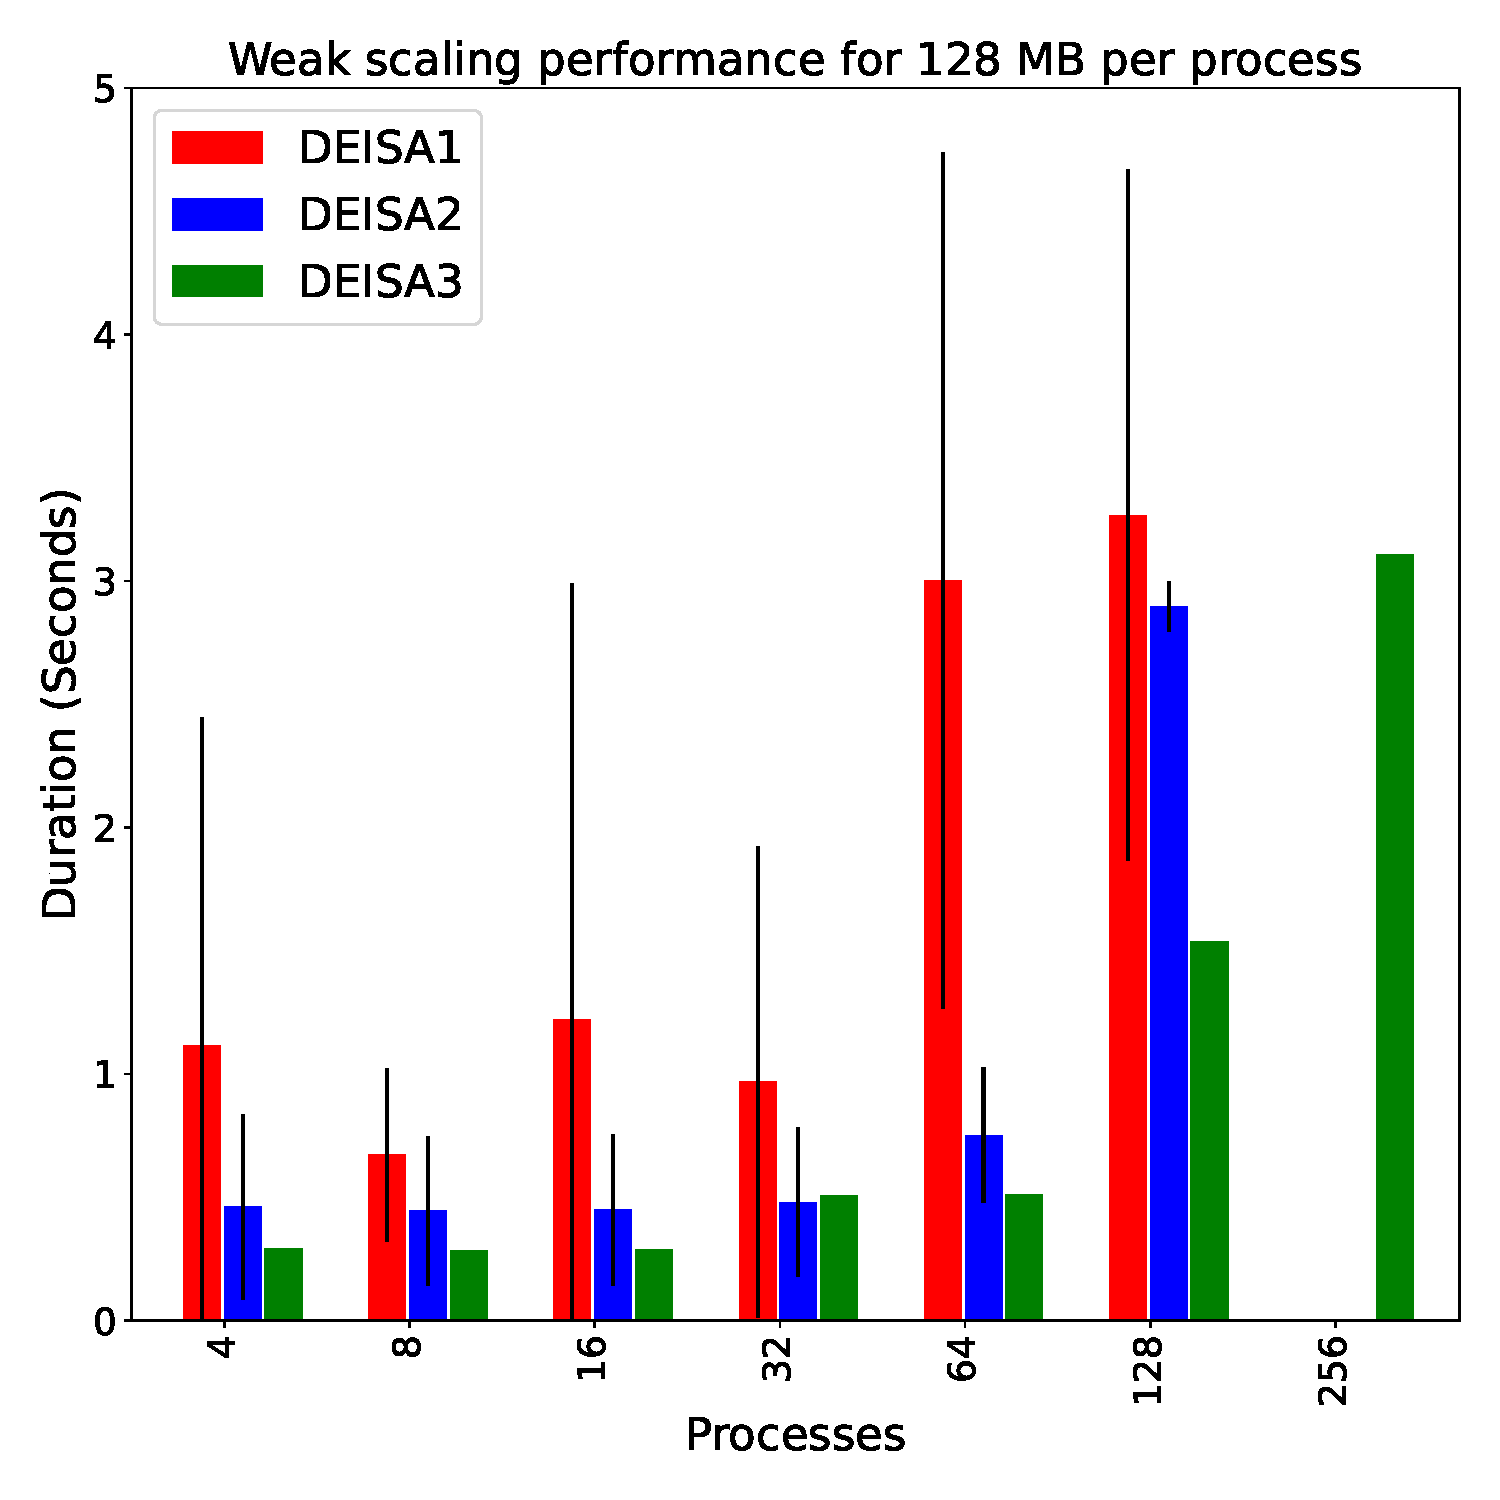
\includegraphics[width=\textwidth, height=\textwidth]{figures/128MB_1vs2vs3.pdf}
         \caption{Average communication times per iteration for 128\,MiB per process}
         \label{fig:X2_128}
     \end{subfigure}
     \hfill
     \begin{subfigure}[b]{0.4\textwidth}
         \centering
         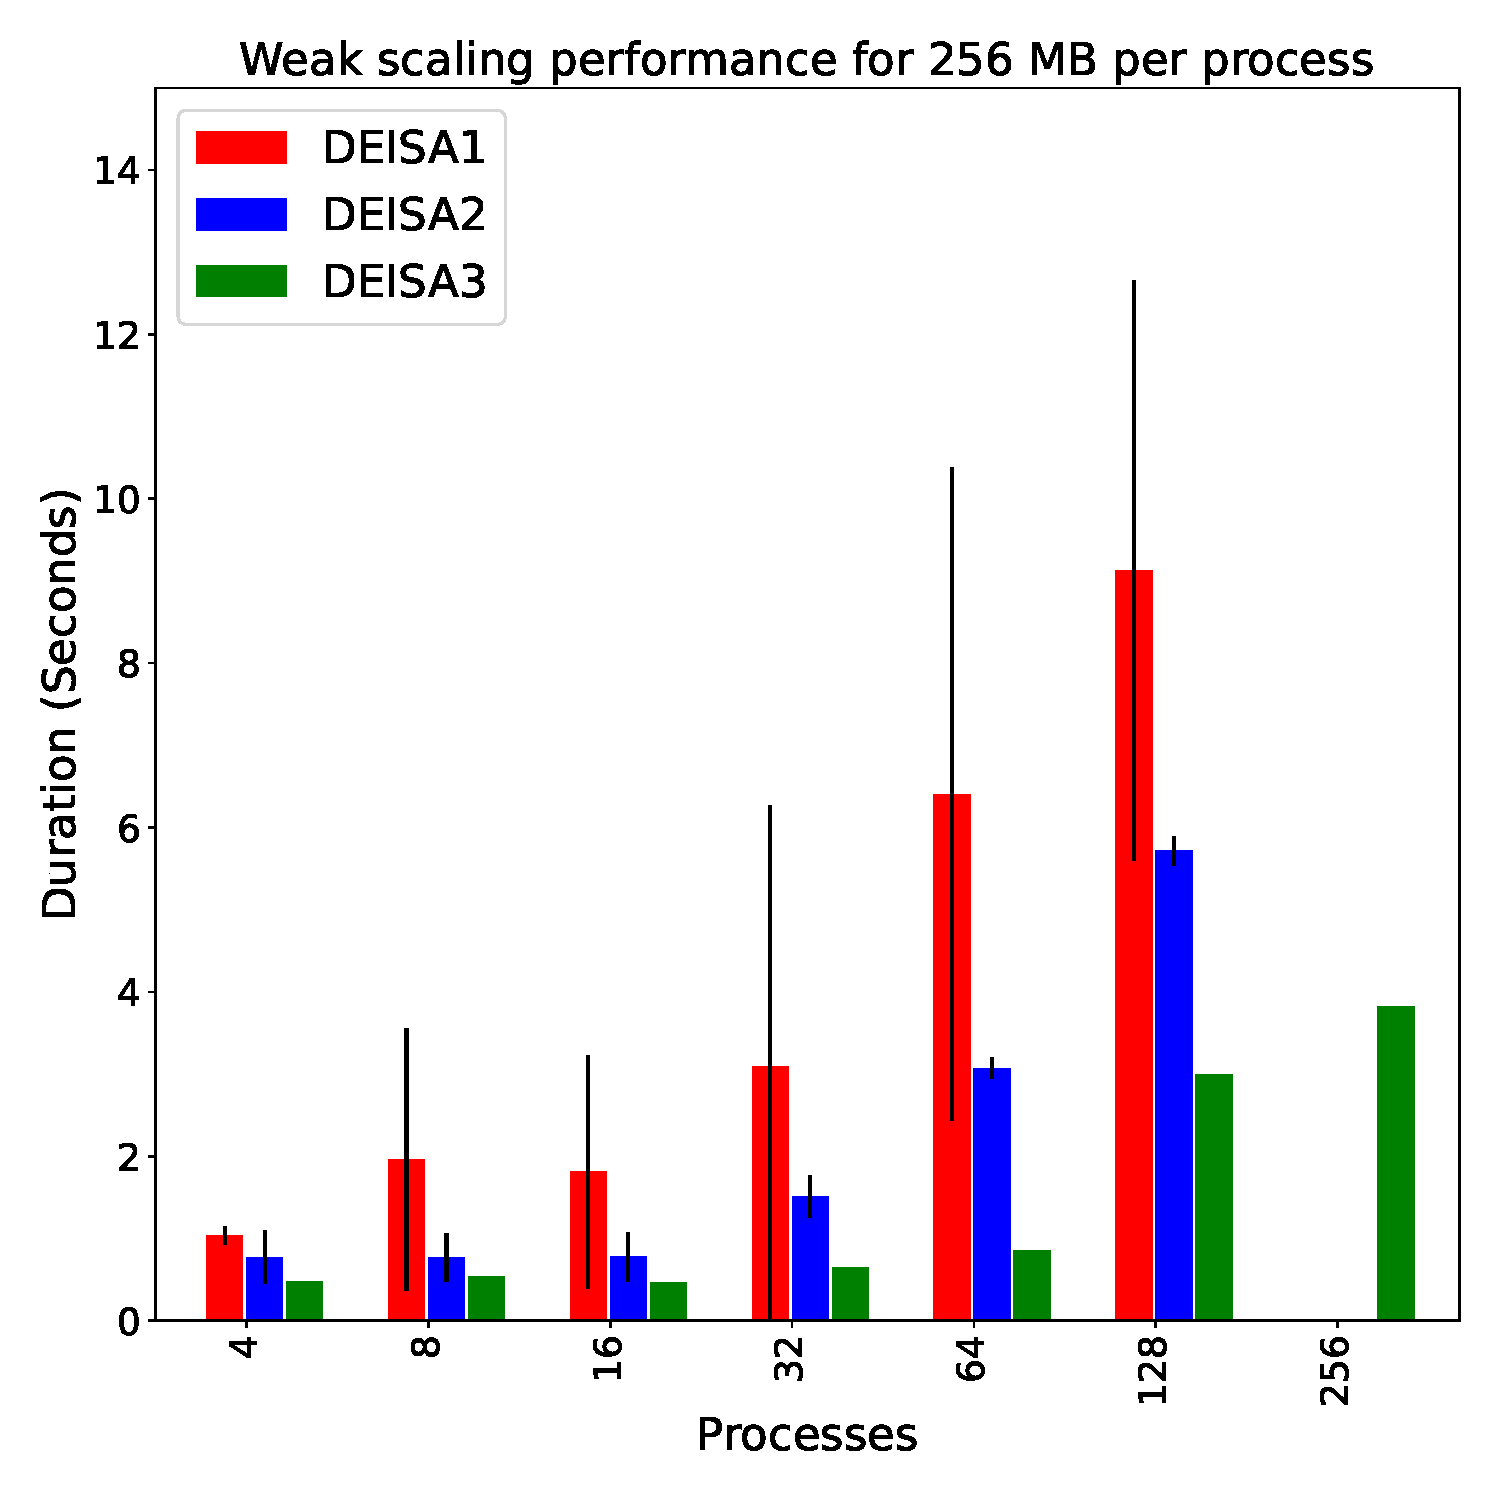
\includegraphics[width=\textwidth, height=\textwidth]{figures/256MB_1vs2vs3.pdf}
         \caption{Average communication times per iteration for 256\,MiB per process}
         \label{fig:X2_256}
     \end{subfigure}
     \vfill
     \begin{subfigure}[b]{0.4\textwidth}
         \centering
         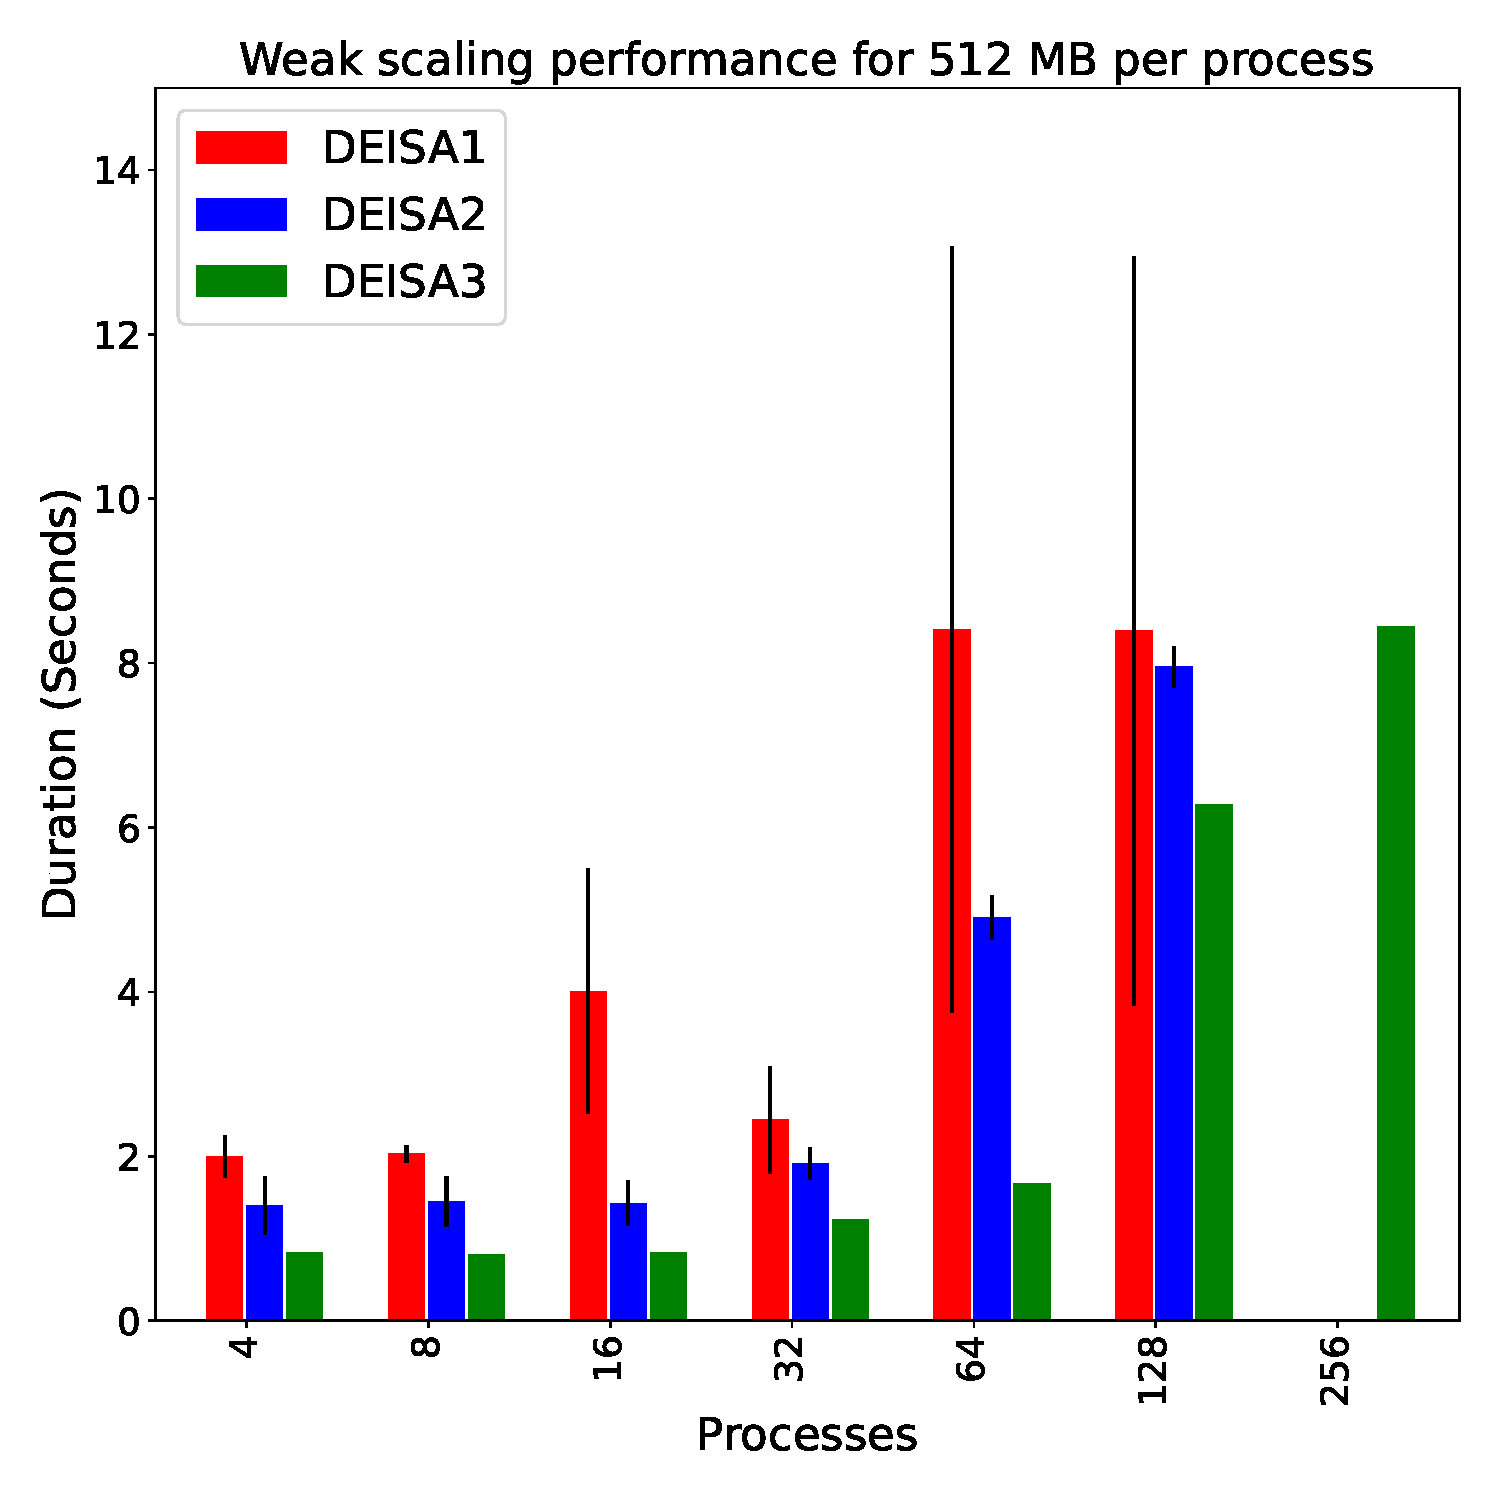
\includegraphics[width=\textwidth, height=\textwidth]{figures/512MB_1vs2vs3.pdf}
         \caption{Average communication times per iteration for 512\,MiB per process}
         \label{fig:X2_512}
     \end{subfigure}
     \hfill
     \begin{subfigure}[b]{0.4\textwidth}
         \centering
         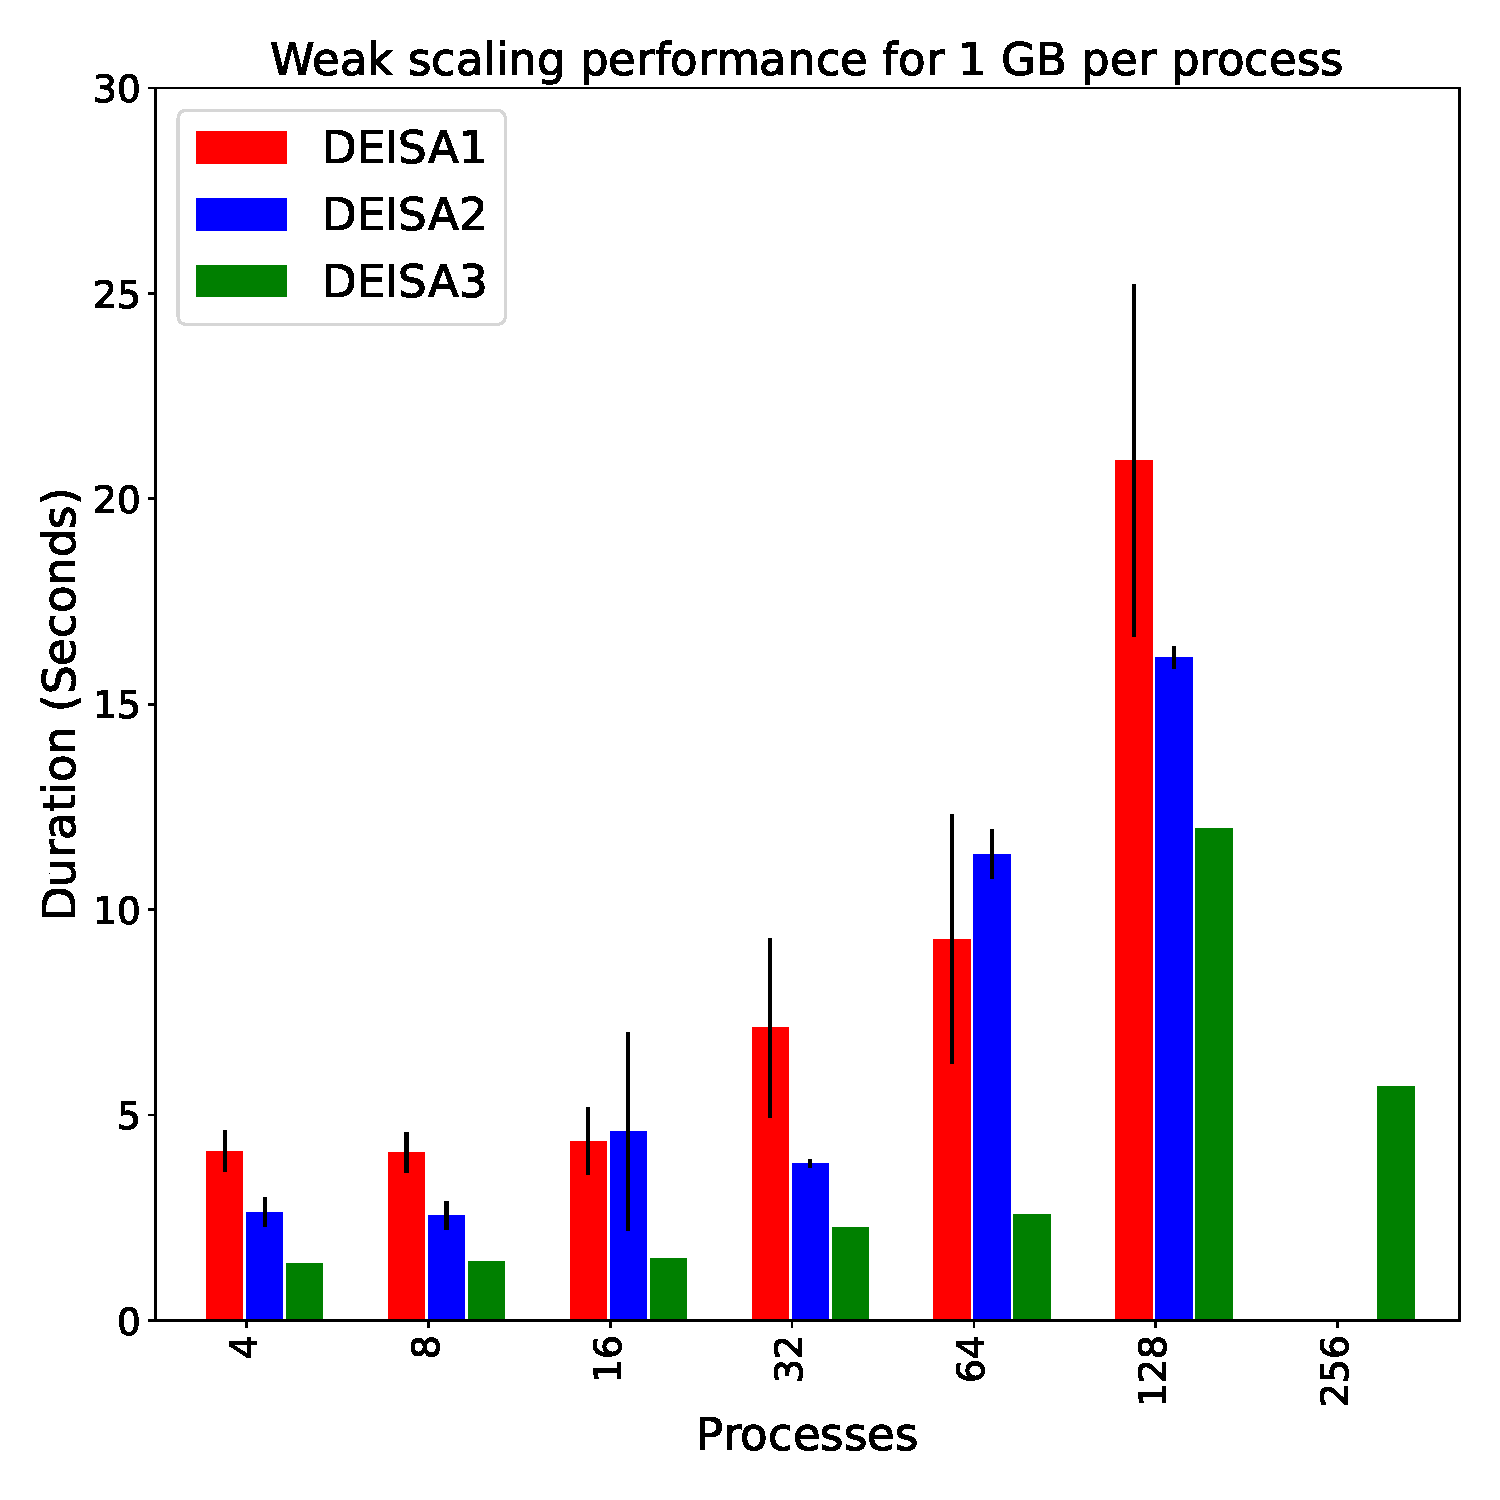
\includegraphics[width=\textwidth, height=\textwidth]{figures/1GB_1vs2vs3.pdf}
         \caption{Average communication times per iteration for 1\,GiB per process}
         \label{fig:X2_1}
     \end{subfigure}
        \caption{Weak scaling average communication for 128\,MiB, 256\,MiB, 512\,MiB  and 1\,GiB per process per iteration for three experiments: the first bar from the left of each scale represents the communication time for the old version of \deisa (in red), the second shows the results for \deisa without contracts (in blue), and the third bar represents results for \deisa full options (in green)}
        \label{fig:perfX2}
\end{figure}


Figure~\ref{fig:perfX2} shows the weak scaling results for the different configurations of \textbf{Experiment III}\ref{XP3}. 
In the subfigure in the top left (Subfigure~\ref{fig:X2_128}), we have fixed the size of the data per MPI process to 128\,MiB, to 256\,MiB in the subfigure in the top right (Subfigure~\ref{fig:X2_256}), to 512\,MiB in the subfigure in the bottom left (Subfigure~\ref{fig:X2_512}) and to 1\,GiB in the bottom right (Subfigure~\ref{fig:X2_1}). 
The x-axis of each subfigure represents the variation of the processes for 4 to 128 for DEISA1 and DEISA2 and for 256 for DEISA3, and y-axis represents the duration in seconds of communication time. 
In each subfigure, we have the three cases of Experiment III\ref{XP3}: the first bar from the left of each scale  is the communication time for DEISA1. The bar in the middle shows results for DEISA2: the new version without contracts and the heartbeat interval set to one minute instead of 5s, in blue. The last bar of each scale shows results for the communication time of the new version of \deisa with contracts activated and the heartbeat interval set to $\infty$.

The represented values are the mean duration over iteration and runs of the maximum value per process. The bar errors are the standard deviation. The standard deviation is not represented for DEISA3 as we do only send the data once every two iterations.

We expect DEISA1 to have the worst performance with more variability (because of the number of metadata we send at each timestep, and the heartbeat interval). DEISA2 would be less variable than DEISA1. 
DEISA3 will perform twice better than DEISA2 and be less variable. 
We have activated the contracts for DEISA3 (Listing~\ref{listderiv}). It prevents the bridges from sending the data to the workers if it is not needed in the analytics. 

Overall, our expectations are true for almost all cases. DEISA1 presents more variability than DEISA2. For all cases, DEISA2 is better than DEISA1 except in Subfigure\ref{fig:X2_1}, when the number of processes is 64. Since we do not observe a big variability, this may be due to the node allocation of this experiment. We will have a look at this in detail in the last part of this discussion.
DEISA3 also shows a strange duration when the number of processes is 128, which we will explore later.

The three versions weak-scale almost perfectly until 64 processes. Then we start seeing an unpredictable variation in the duration for DEISA2 and DEISA3.  

This may be due to the physical distance of simulation nodes from the workers and the scheduler nodes, which may vary along allocations and affect the performance. 

The Skylake partition's compute nodes are connected through an EDR InfiniBand network in a pruned fat-tree topology. 
To simplify the topology, we suppose that we have four nodes: $N_1, N_2, N_3, N_4$. Every $2$ nodes are related to a switch $L_2$ where we have $N_1 $ with $ N_2$ and $N_3 $ with $ N_4$, then the two switches $L_2$ are related to a $L_1$ switch. 
Figure~\ref{fig:fatTreeTopo} shows the difference between a fat tree topology and a pruned fat tree topology which is used the topology of the Skylake partition we are using. The fat tree topology has 200\,Gib in the switch $L_1$; this maintains the 100\,Gib over all the nodes. However, in the pruned fat tree topology, a 100\,Gib link has been used, which makes communications between $N_1$ and $[N_3, N_4]$  or  $N_2$ and $[N_3, N_4]$ potentially longer, and vice versa.    

\begin{figure}
     \centering
     \begin{subfigure}[b]{0.45\textwidth}
         \centering
         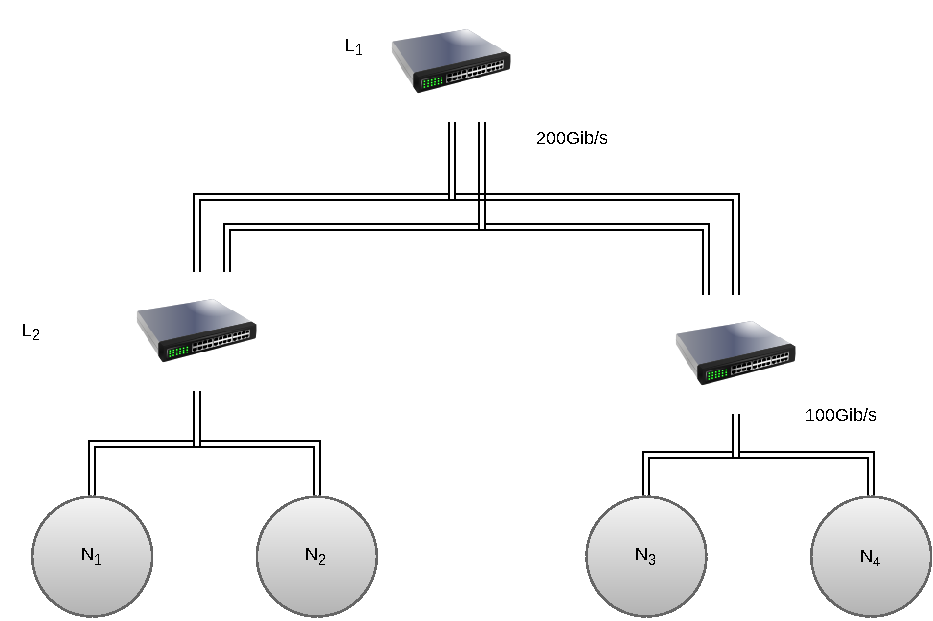
\includegraphics[width=\textwidth, height=\textwidth]{figures/fatTree.pdf}
         \caption{Fat Tree topology}
         \label{fig:fat}
     \end{subfigure}
     \hfill
     \begin{subfigure}[b]{0.45\textwidth}
         \centering
         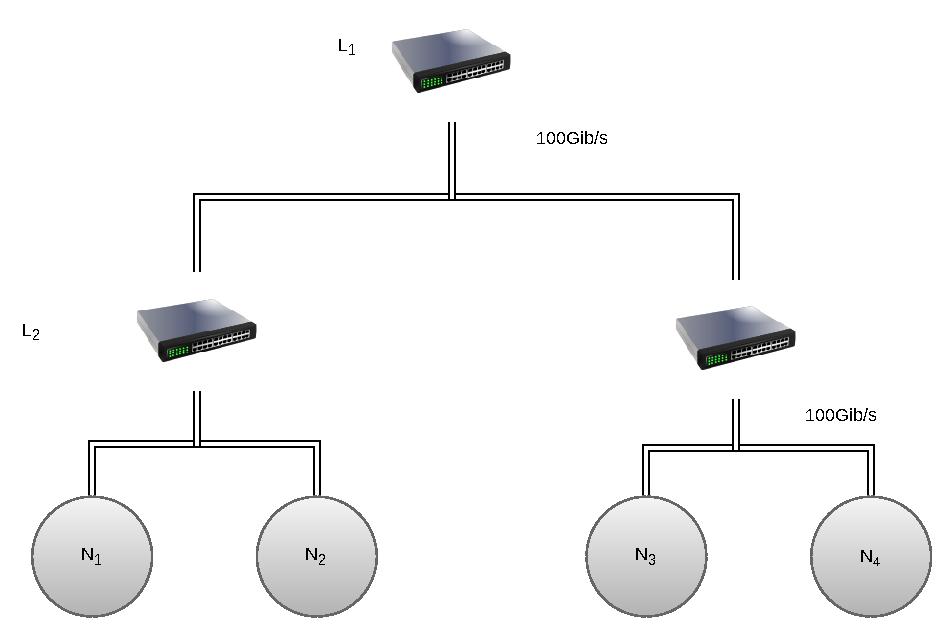
\includegraphics[width=\textwidth, height=\textwidth]{figures/PrunedFat.pdf}
         \caption{Pruned Fat Tree topology}
         \label{fig:prunedfat}
     \end{subfigure}
        \caption{Fat Tree versus Pruned Fat Tree topology}
        \label{fig:fatTreeTopo}
\end{figure}

If the scheduler, which is always in the first node of our allocation, is related to a different switch than some of the simulation nodes, the time to send the messages will vary because of the distance (the number of switches that a message has to go through before getting to the workers and the scheduler) and the bandwidth may get smaller when we go higher in the tree. 

We have investigated this variability by checking the mean duration of the communications per rank for DEISA3 and show the results in Figure~\ref{fig:variability}.
We have fixed the number of processes to 256 and varied the size of the data per process: 128\,MiB, 256\,MiB, 512MiB and 1\,GiB. We have separated the results we got from each run. Each line in the subfigures corresponds to a fixed size of the data. 
We have submitted the runs independently, so we do not have control over the allocated nodes, but we may have the same allocation. 
The x-axis of each subfigure represents the MPI ranks, and the y-axis shows the mean value per rank over iterations (the black line). The standard deviation over iterations is represented as a red band. 
First of all, we notice that there is variability over the 3 runs for specific data size, but overall we do not really notice the red band, so there is minimal variability over iteration. 
In some subfigures, we have the same pattern of variability, for instance: 
Subfigure~\ref{fig:E2_128} and Subfigure~\ref{fig:E3_128}, Subfigure~\ref{fig:E2_256} and Subfigure~\ref{fig:E2_256}, Subfigure~\ref{fig:E2_512} and Subfigure~\ref{fig:E2_512}, 
Subfigure~\ref{fig:E2_1} and Subfigure~\ref{fig:E2_1}. 
This makes us think that they may have the same allocations of at least nodes connected to the same switches. 
We also notice the same patterns even when the size of the data changes, for instance: Subfigure~\ref{fig:E2_512}, Subfigure~\ref{fig:E3_512}, Subfigure~\ref{fig:E1_1}, Subfigure~\ref{fig:E2_1} and Subfigure~\ref{fig:E3_1} have all of them the same variability pattern. 
We have checked the logs and found that all of the four experiments in  Subfigure~\ref{fig:E2_512}, Subfigure~\ref{fig:E3_512}, Subfigure~\ref{fig:E2_1} and Subfigure~\ref{fig:E3_1} have the exact same allocation, thus the similarity in the variations. Subfigure~\ref{fig:E1_1} allocation differs in two nodes than the four others.
We had a look at the topology of the nodes in the Skylake partition (that we can not publish here) and found that the nodes of the previous five experiments are connected to two different switches, which may explain some of the observed variability over processes. 
Note that the scheduler is launched in the first node of the allocation, the client in the second node, the workers are launched starting from the third node, and then the simulation processes are launched in the rest of the nodes. So here, in this particular case, the scheduler, the client, the workers and some of the processes are connected to the same switch, and the rest of the processes are in the other switch. The centralized scheduler worsens the performance.

\begin{figure}
     \centering
     \begin{subfigure}[b]{0.3\textwidth}
         \centering
         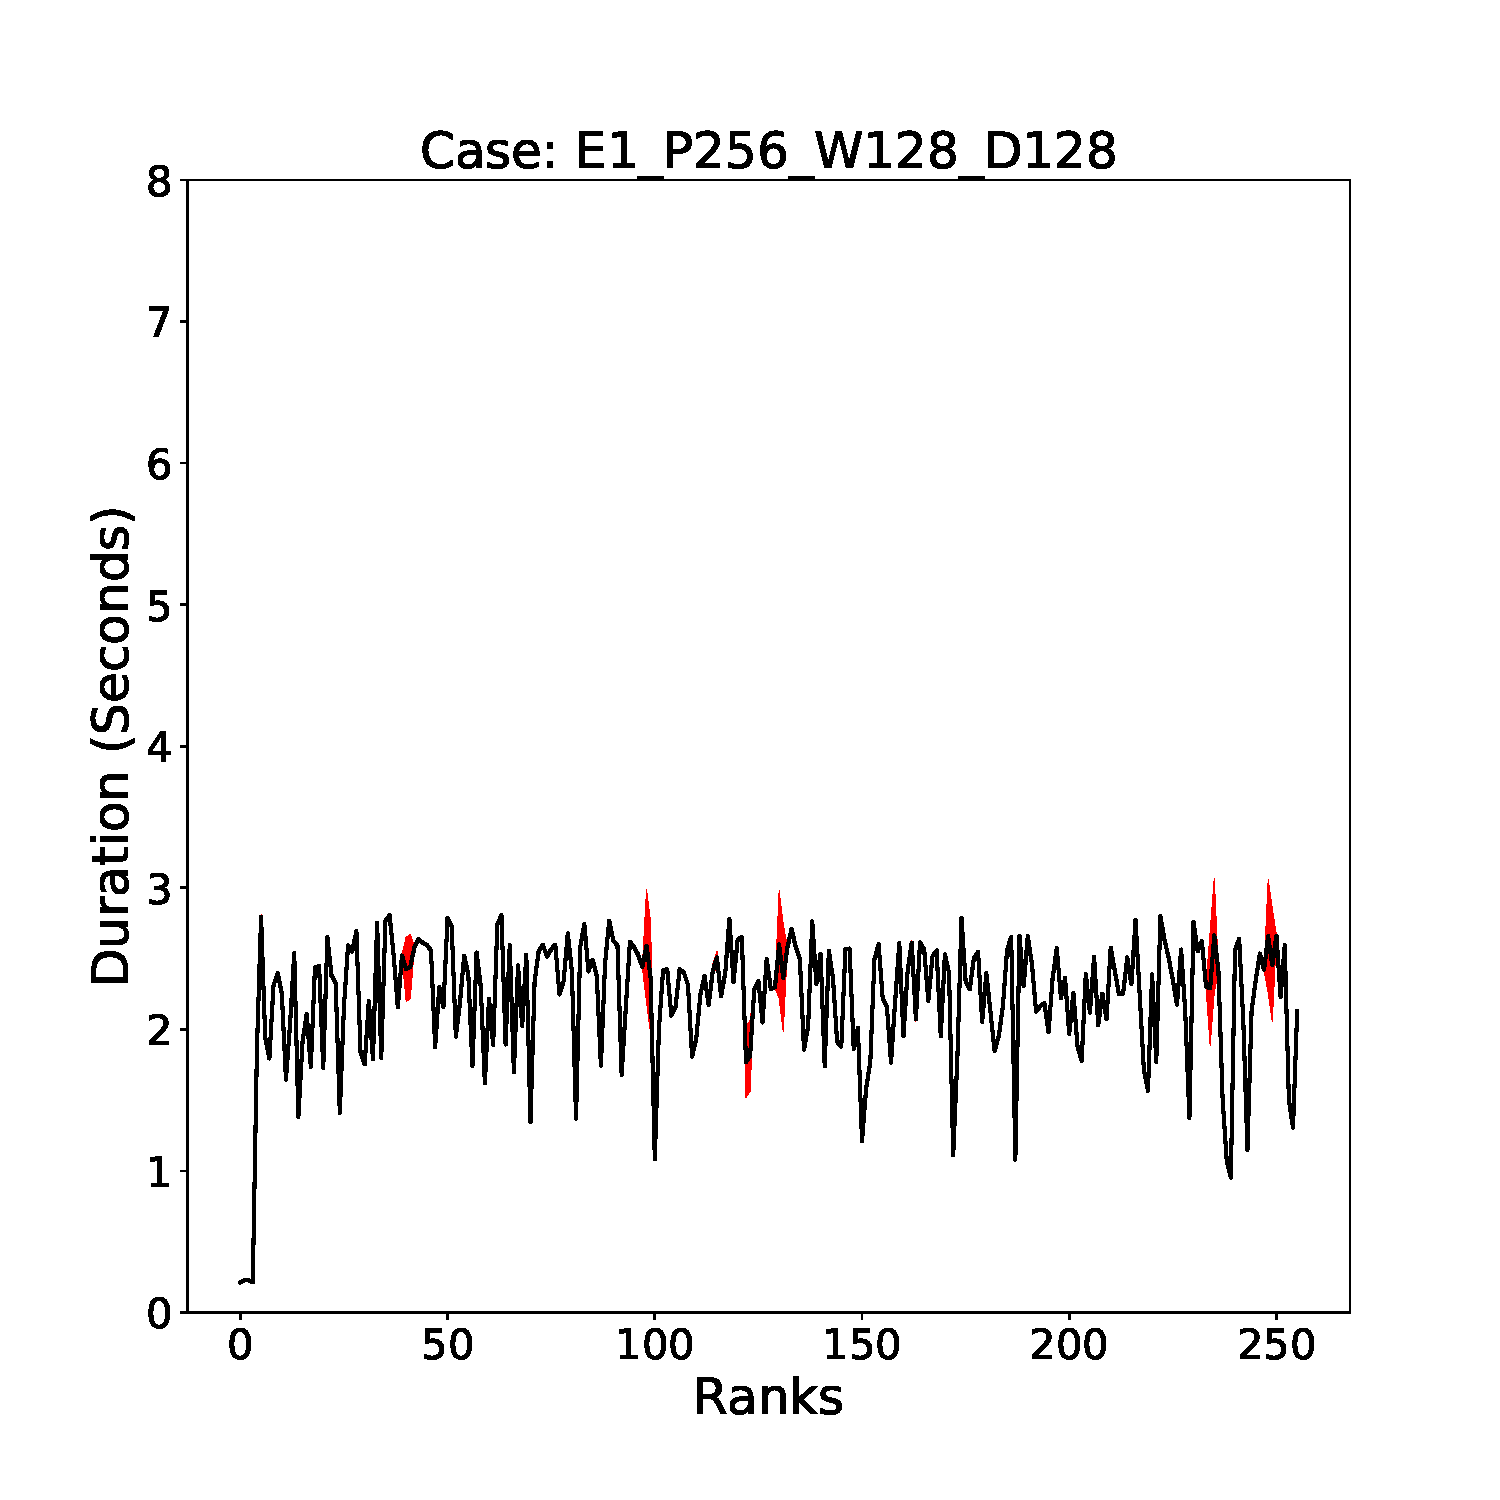
\includegraphics[width=\textwidth, height=\textwidth]{figures/E1_P256_W128_D128.pdf}
         \caption{Run\,1, 128\,MiB per process}
         \label{fig:E1_128}
     \end{subfigure}
     \hfill
     \begin{subfigure}[b]{0.3\textwidth}
         \centering
         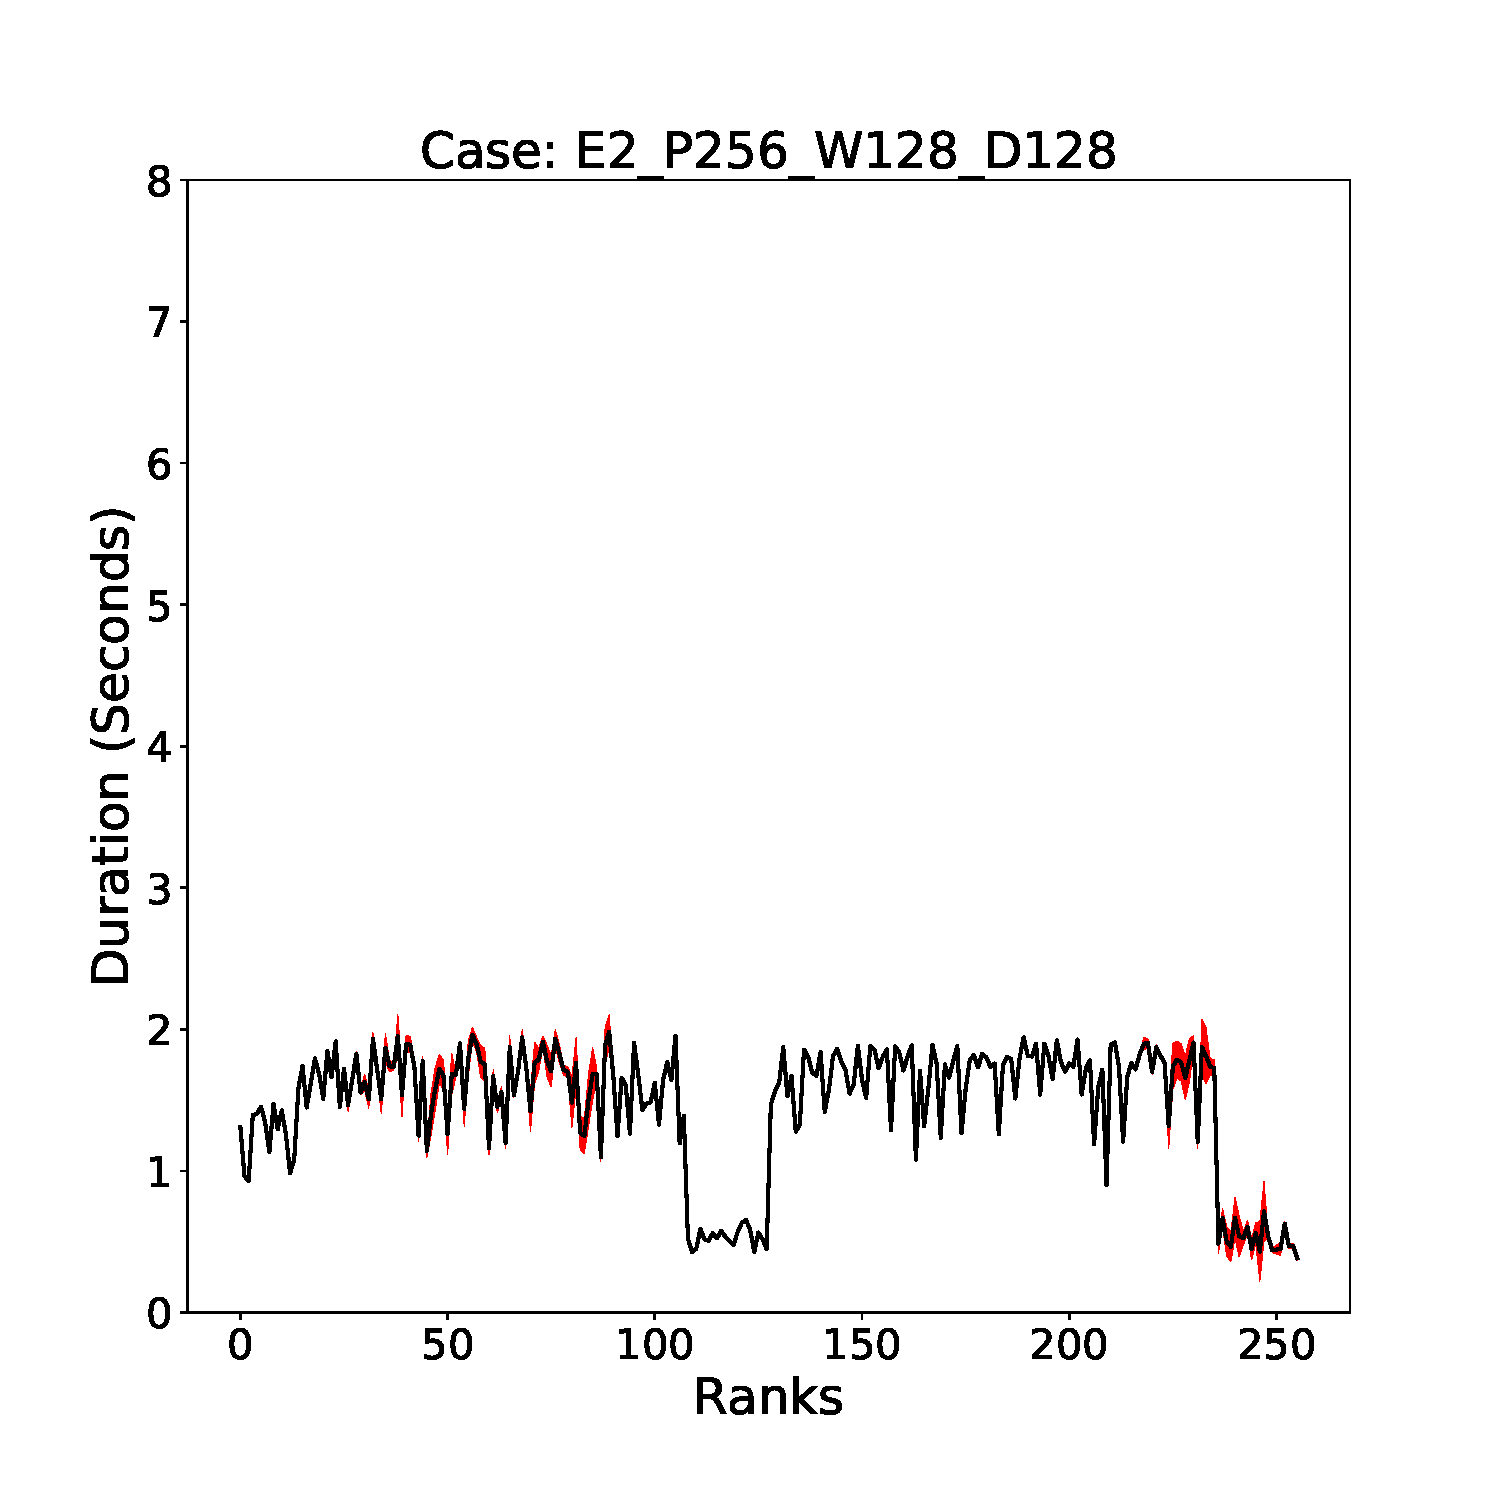
\includegraphics[width=\textwidth, height=\textwidth]{figures/E2_P256_W128_D128.pdf}
         \caption{Run\,2, 128\,MiB per process}
         \label{fig:E2_128}
     \end{subfigure}
      \hfill
     \begin{subfigure}[b]{0.3\textwidth}
         \centering
         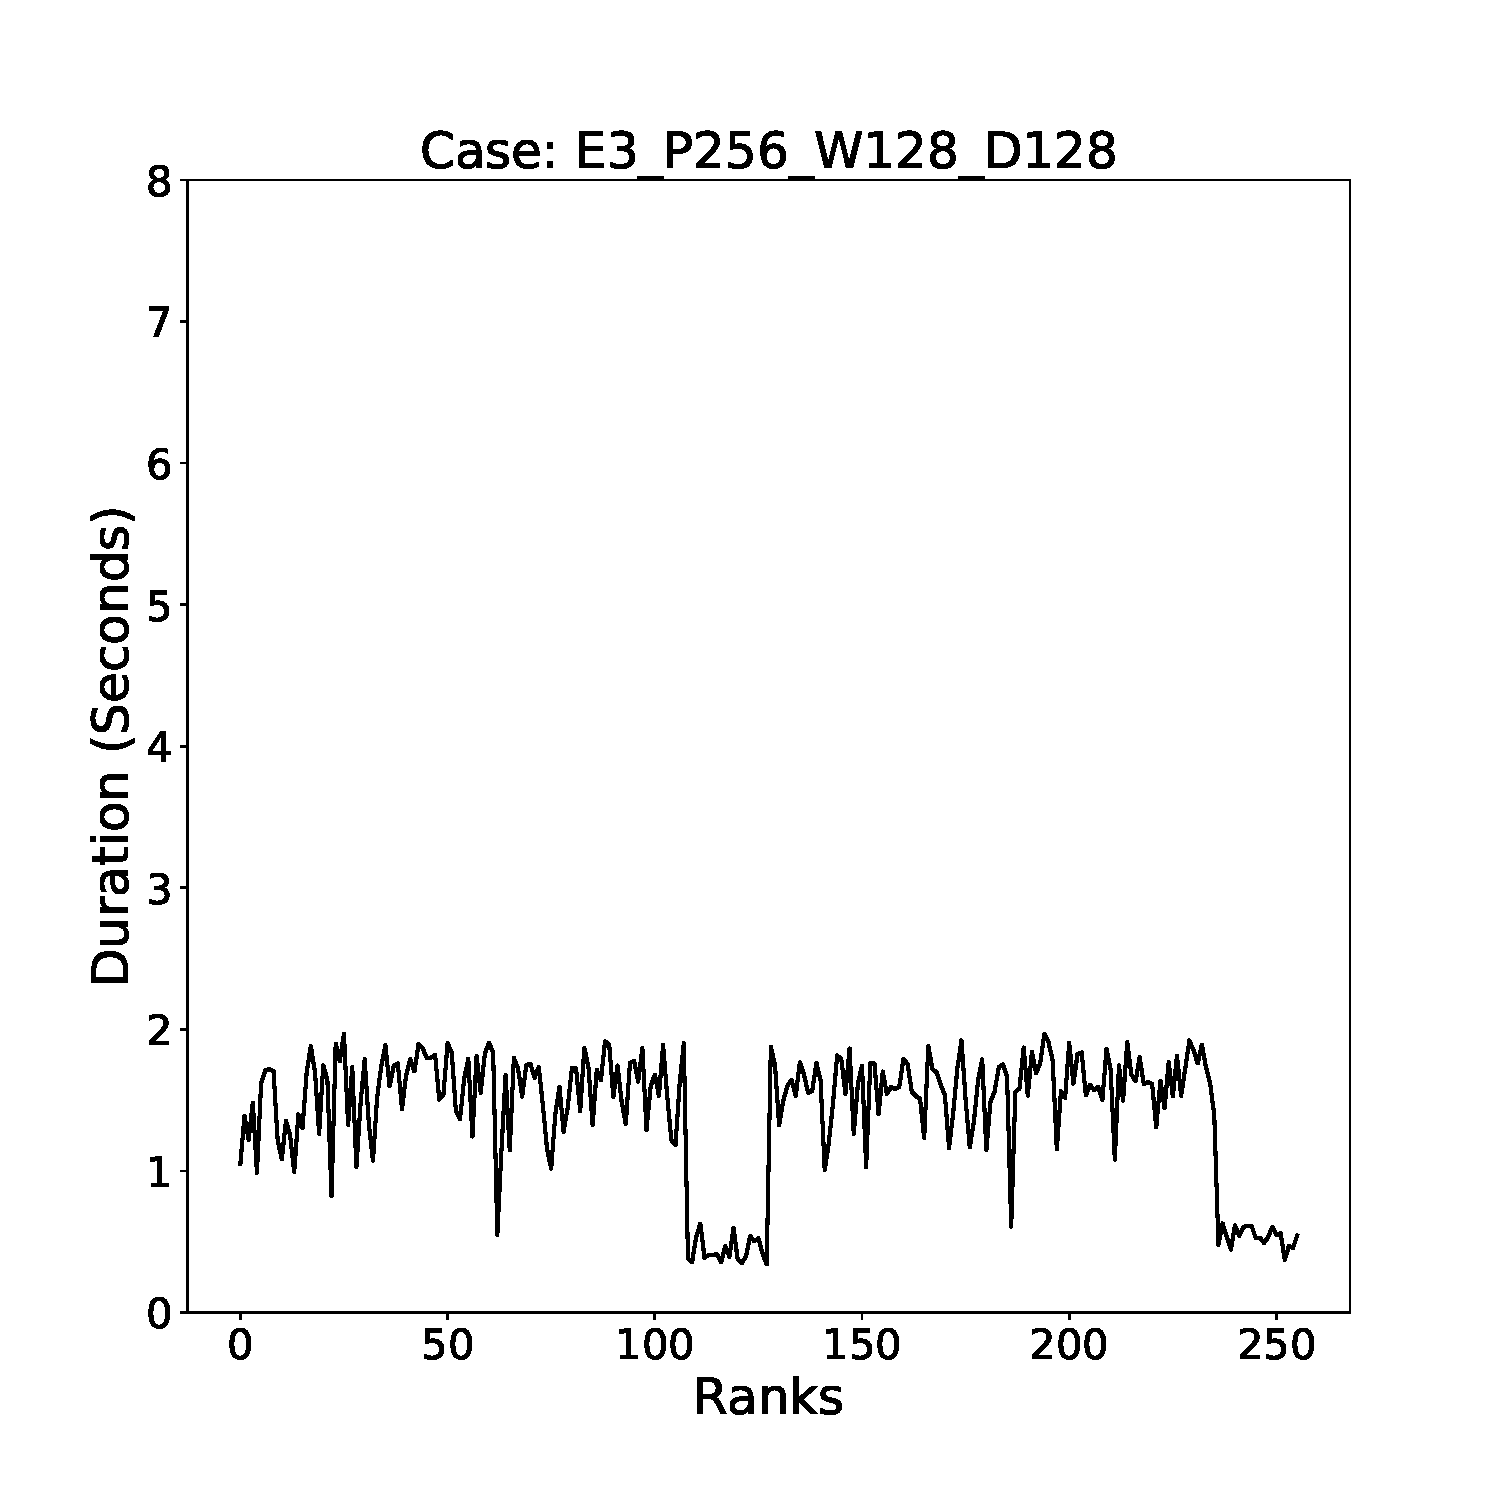
\includegraphics[width=\textwidth, height=\textwidth]{figures/E3_P256_W128_D128.pdf}
         \caption{Run\,3, 128\,MiB per process}
         \label{fig:E3_128}
     \end{subfigure}
     \vfill
     \begin{subfigure}[b]{0.3\textwidth}
         \centering
         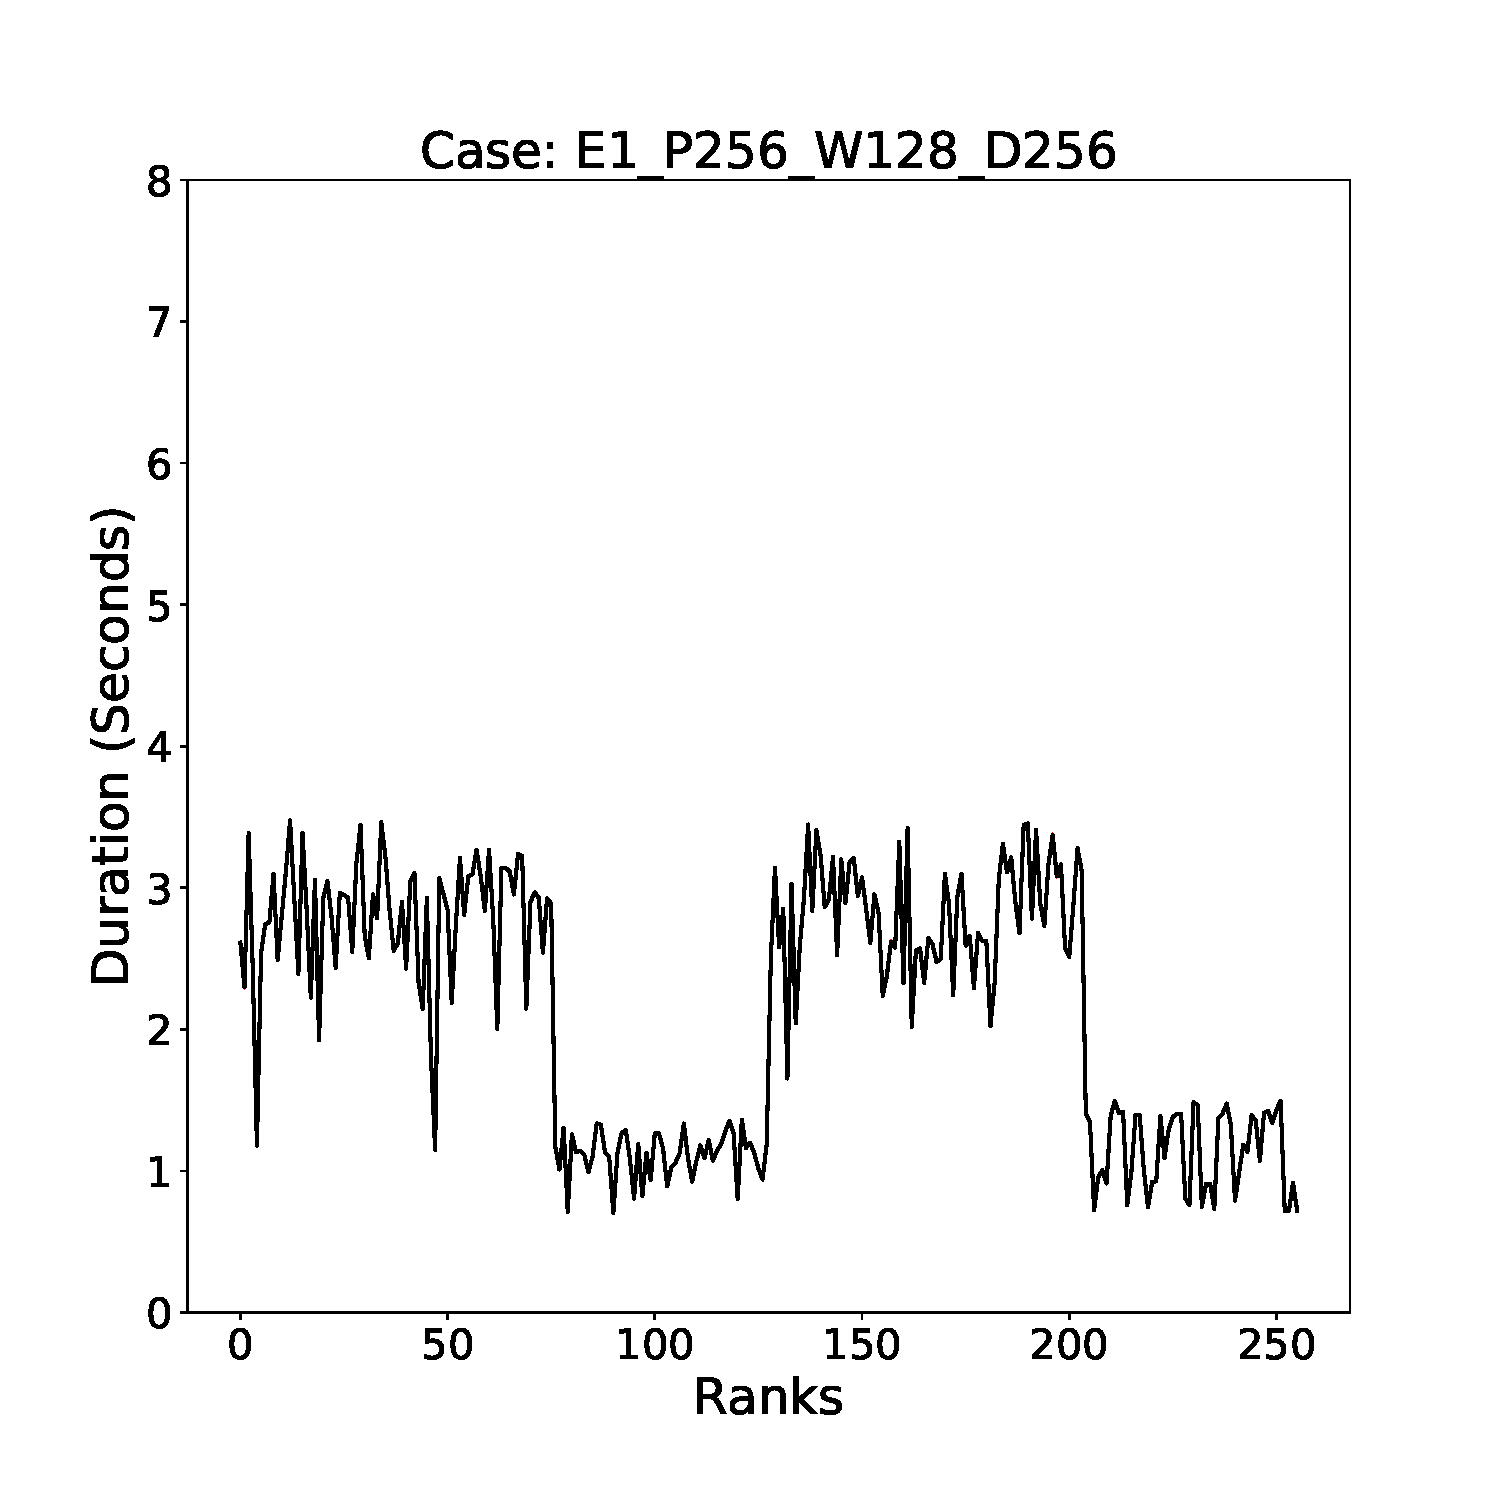
\includegraphics[width=\textwidth, height=\textwidth]{figures/E1_P256_W128_D256.pdf}
         \caption{Run\,1, 256\,MiB per process }
         \label{fig:E1_256}
     \end{subfigure}
     \hfill
     \begin{subfigure}[b]{0.3\textwidth}
         \centering
         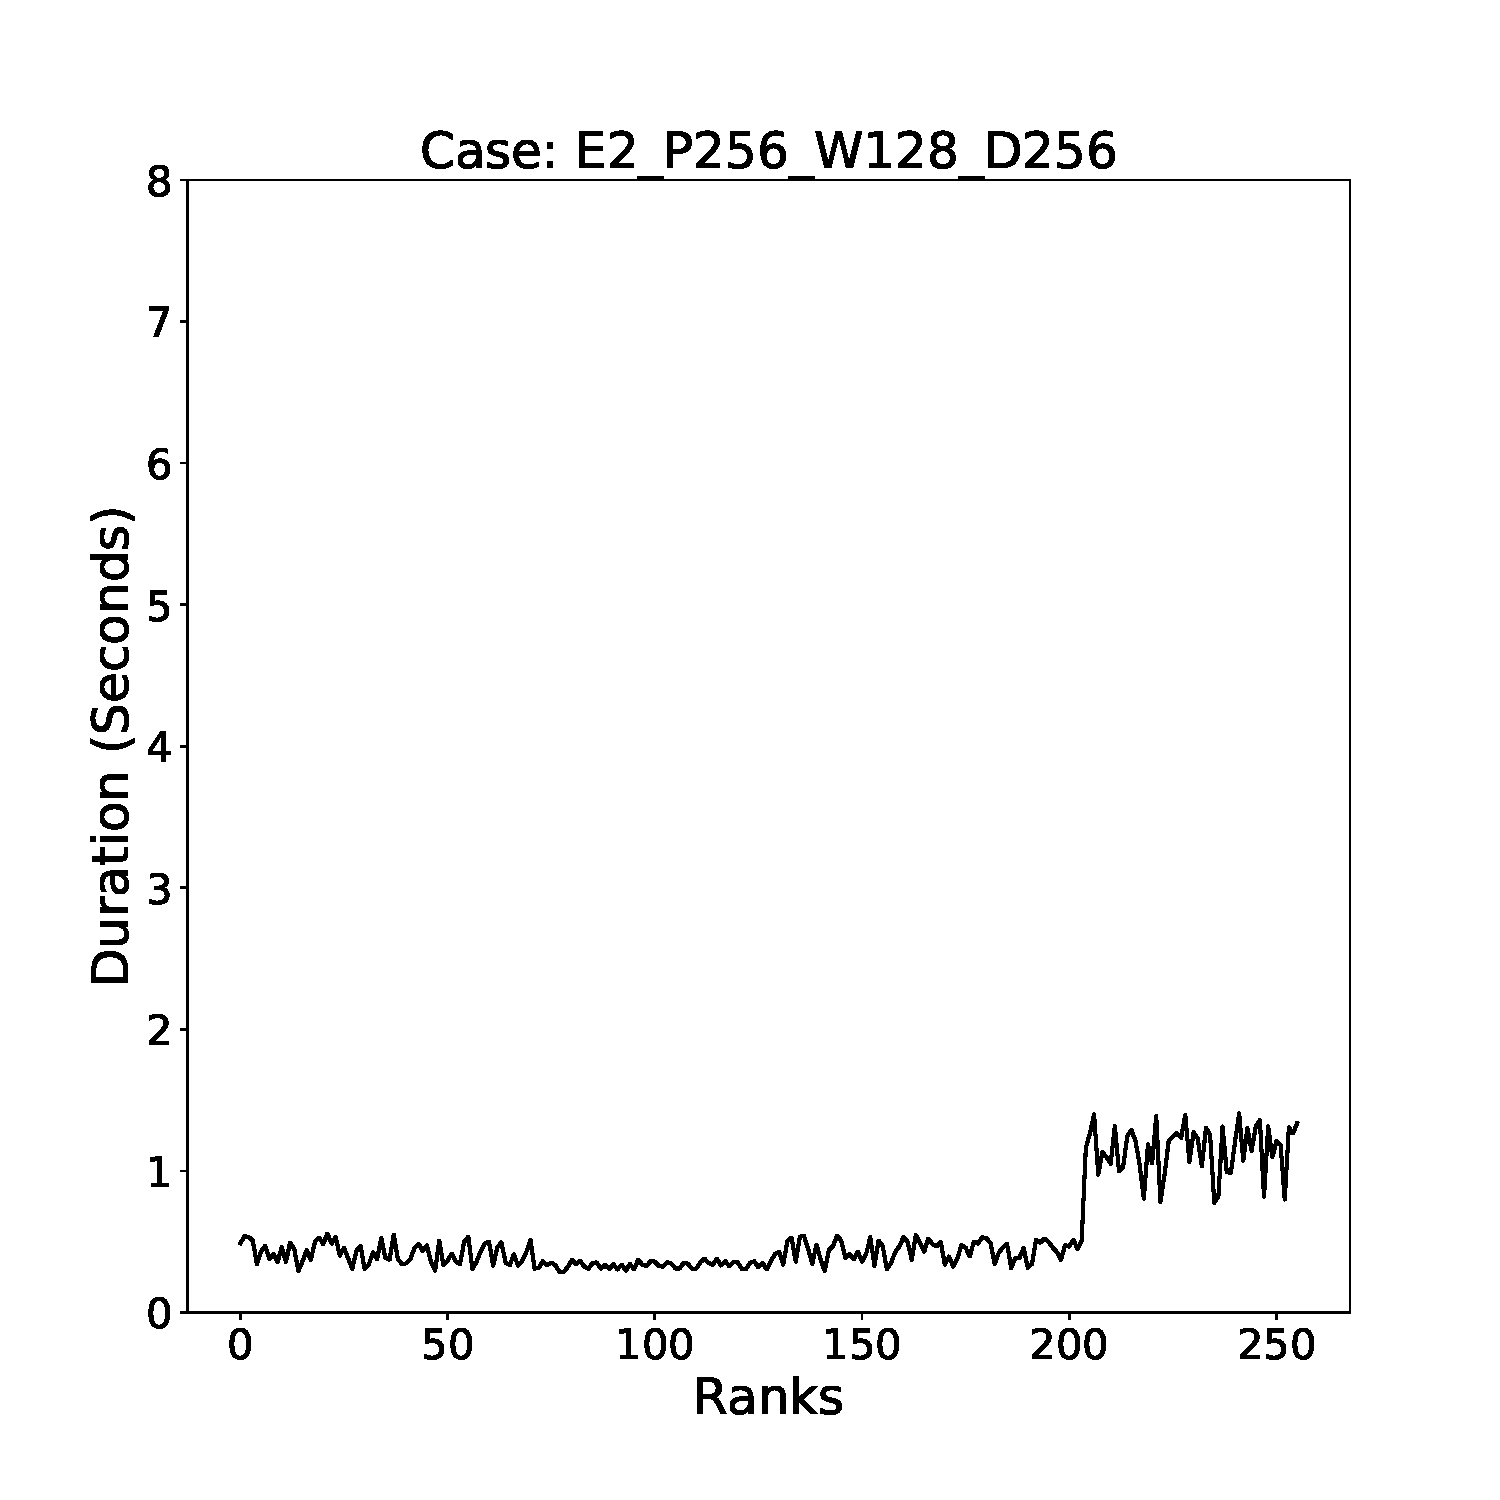
\includegraphics[width=\textwidth, height=\textwidth]{figures/E2_P256_W128_D256.pdf}
         \caption{Run\,2, 256\,MiB per process}
         \label{fig:E2_256}
     \end{subfigure}
      \hfill
     \begin{subfigure}[b]{0.3\textwidth}
         \centering
         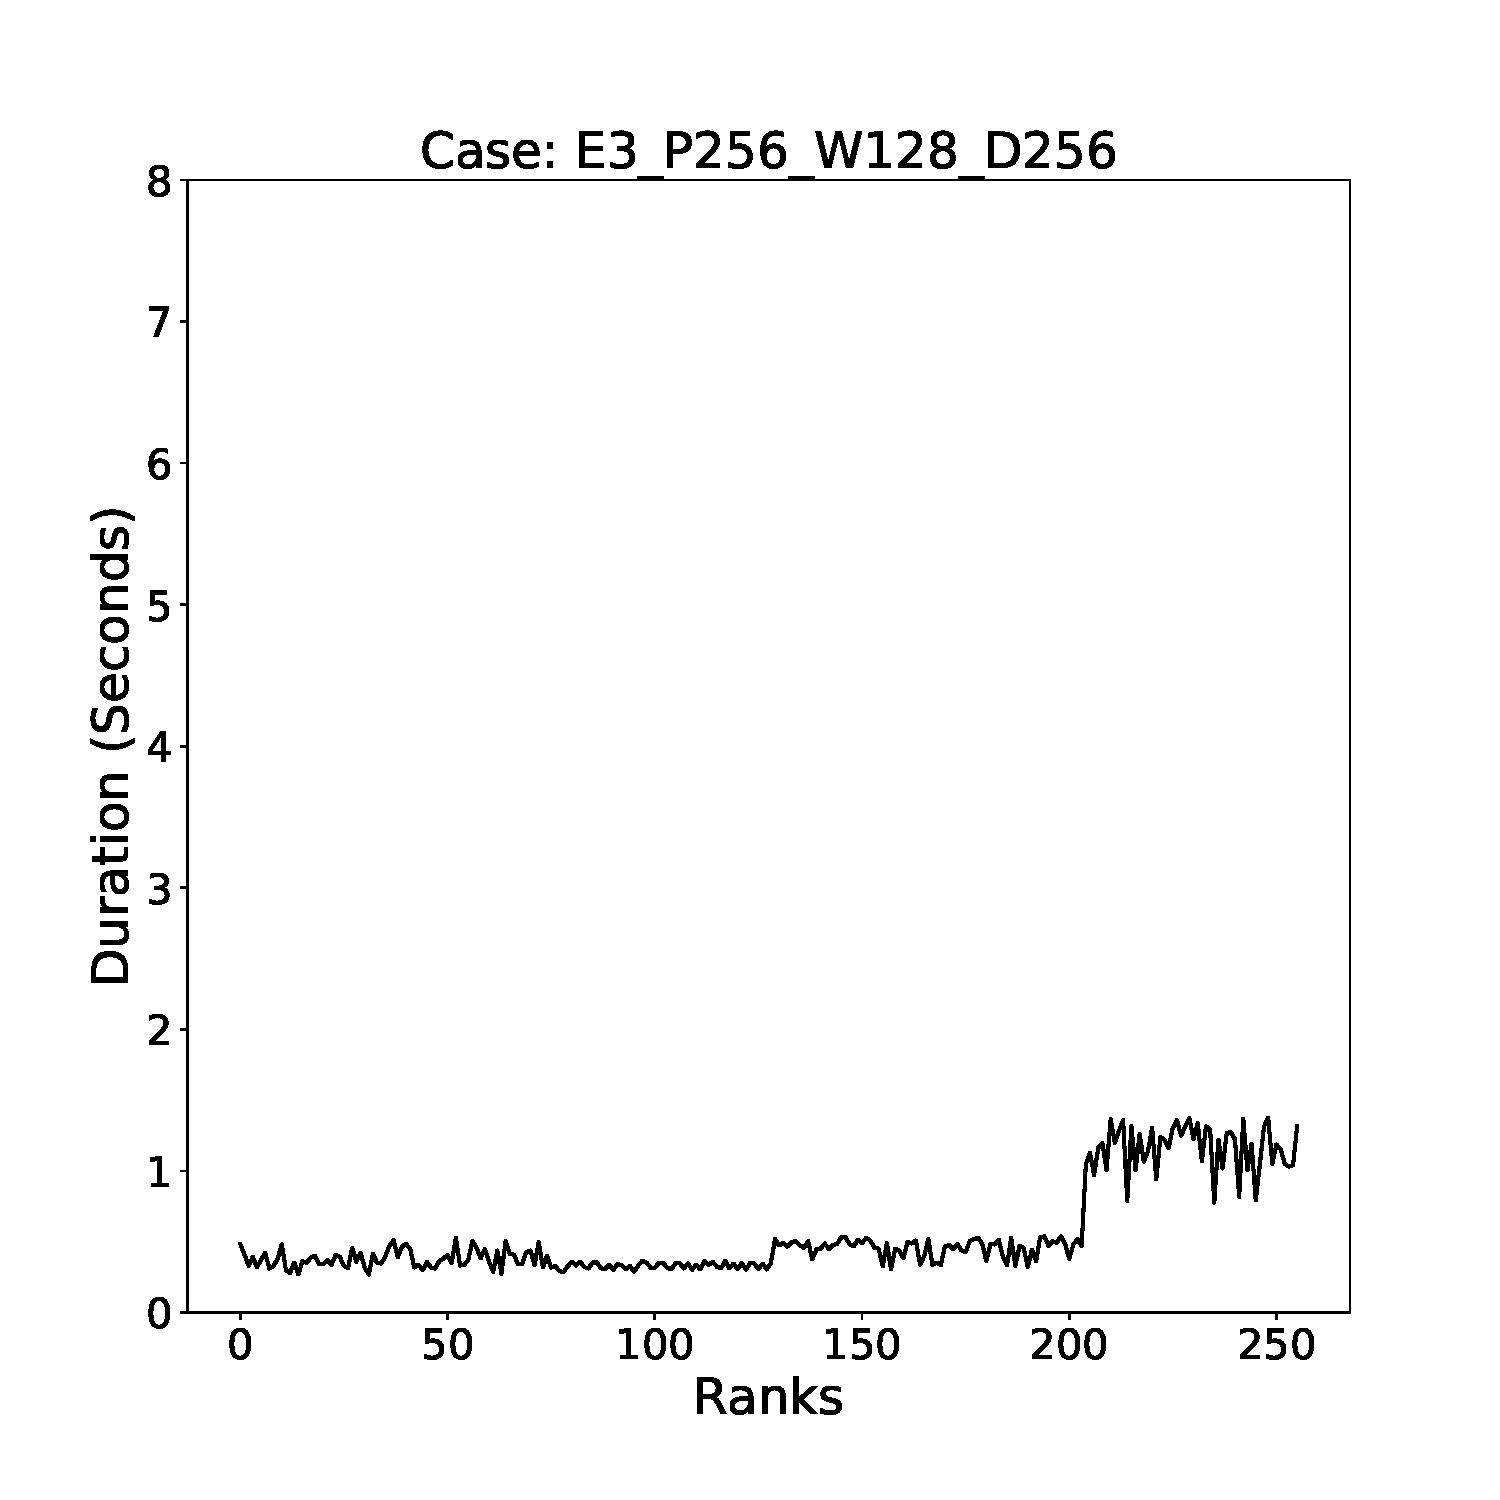
\includegraphics[width=\textwidth, height=\textwidth]{figures/E3_P256_W128_D256.pdf}
         \caption{Run\,3, 256\,MiB per process}
         \label{fig:E3_256}
     \end{subfigure}
     \vfill
          \begin{subfigure}[b]{0.3\textwidth}
         \centering
         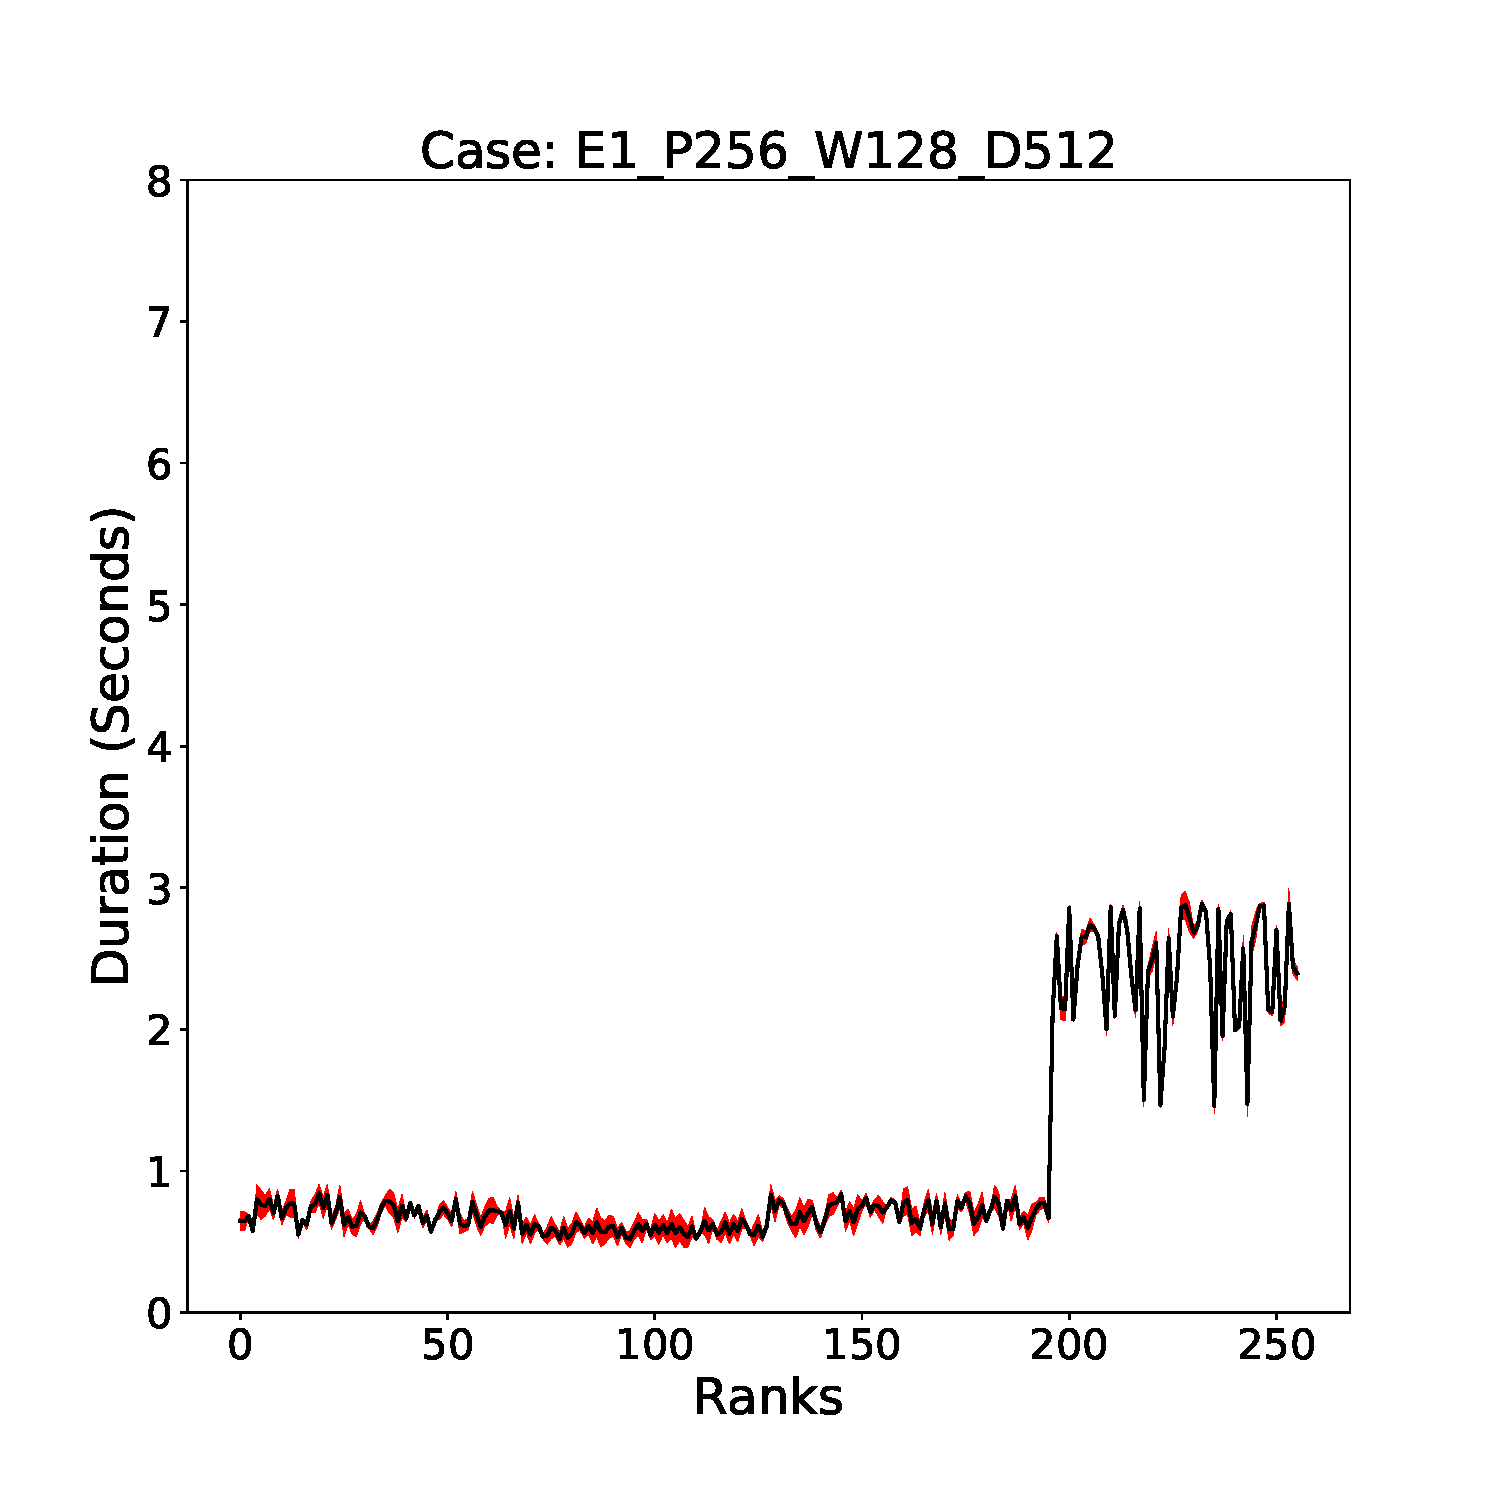
\includegraphics[width=\textwidth, height=\textwidth]{figures/E1_P256_W128_D512.pdf}
         \caption{Run\,1, 512\,MiB per process}
         \label{fig:E1_512}
     \end{subfigure}
     \hfill
     \begin{subfigure}[b]{0.3\textwidth}
         \centering
         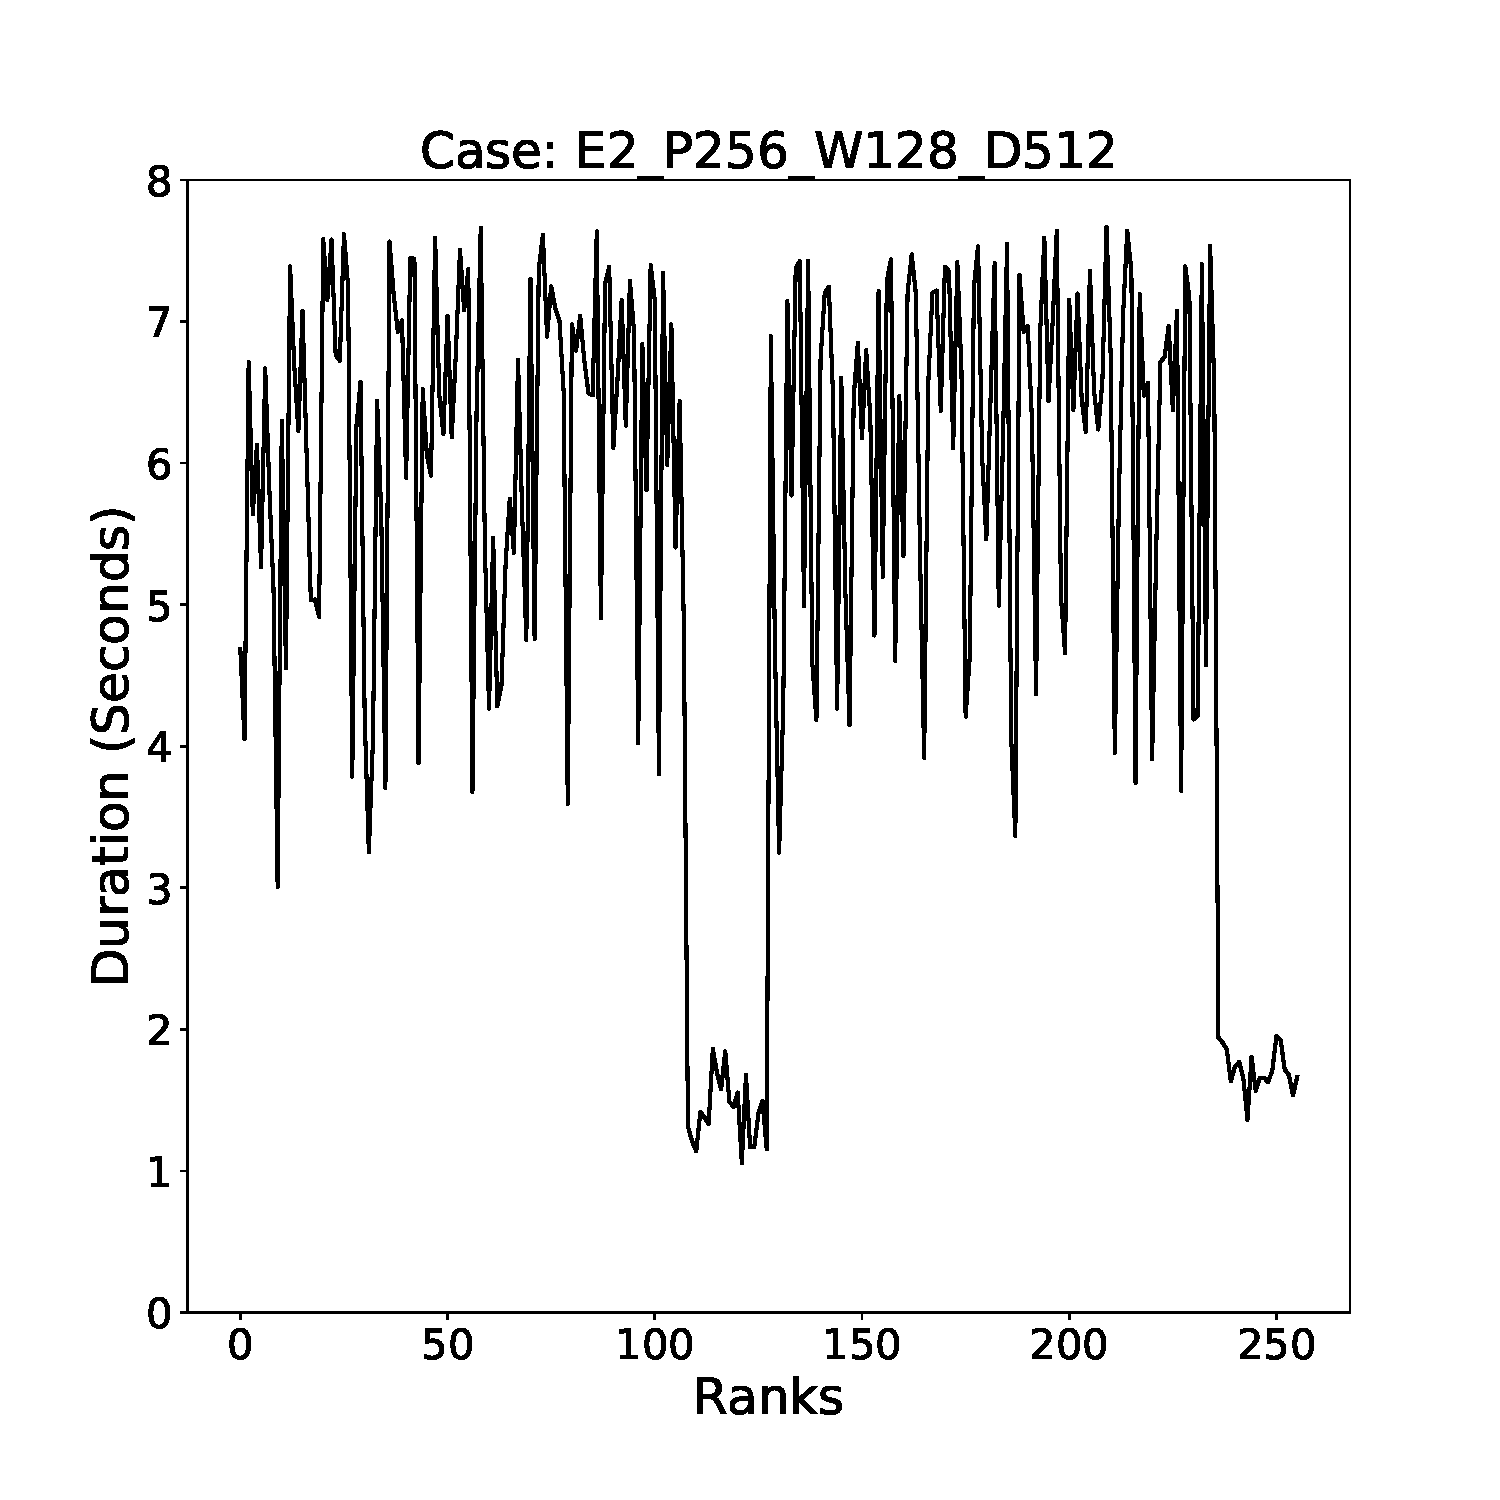
\includegraphics[width=\textwidth, height=\textwidth]{figures/E2_P256_W128_D512.pdf}
         \caption{Run\,2, 512\,MiB per process}
         \label{fig:E2_512}
     \end{subfigure}
      \hfill
     \begin{subfigure}[b]{0.3\textwidth}
         \centering
         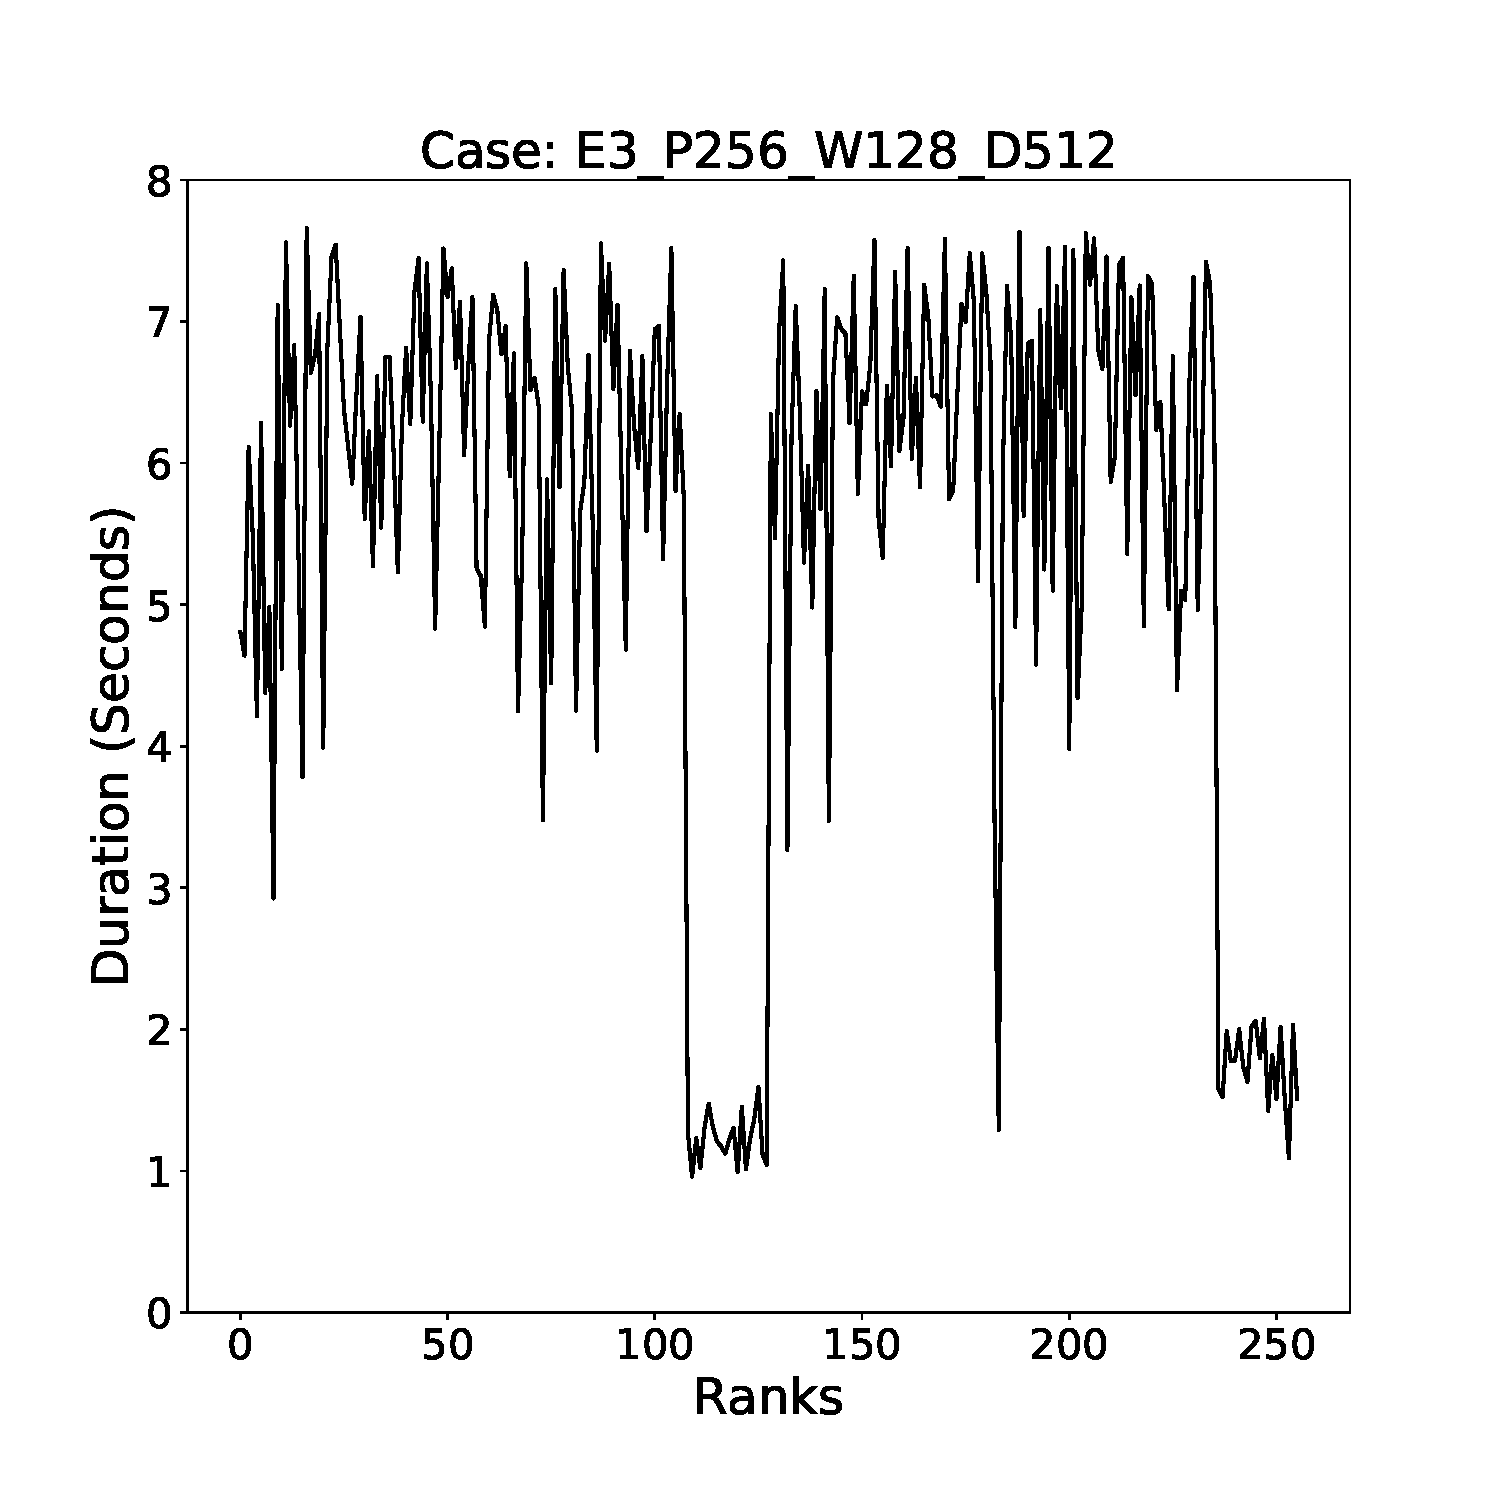
\includegraphics[width=\textwidth, height=\textwidth]{figures/E3_P256_W128_D512.pdf}
         \caption{Run\,3, 512\,MiB per process}
         \label{fig:E3_512}
     \end{subfigure}
     \vfill
          \begin{subfigure}[b]{0.3\textwidth}
         \centering
         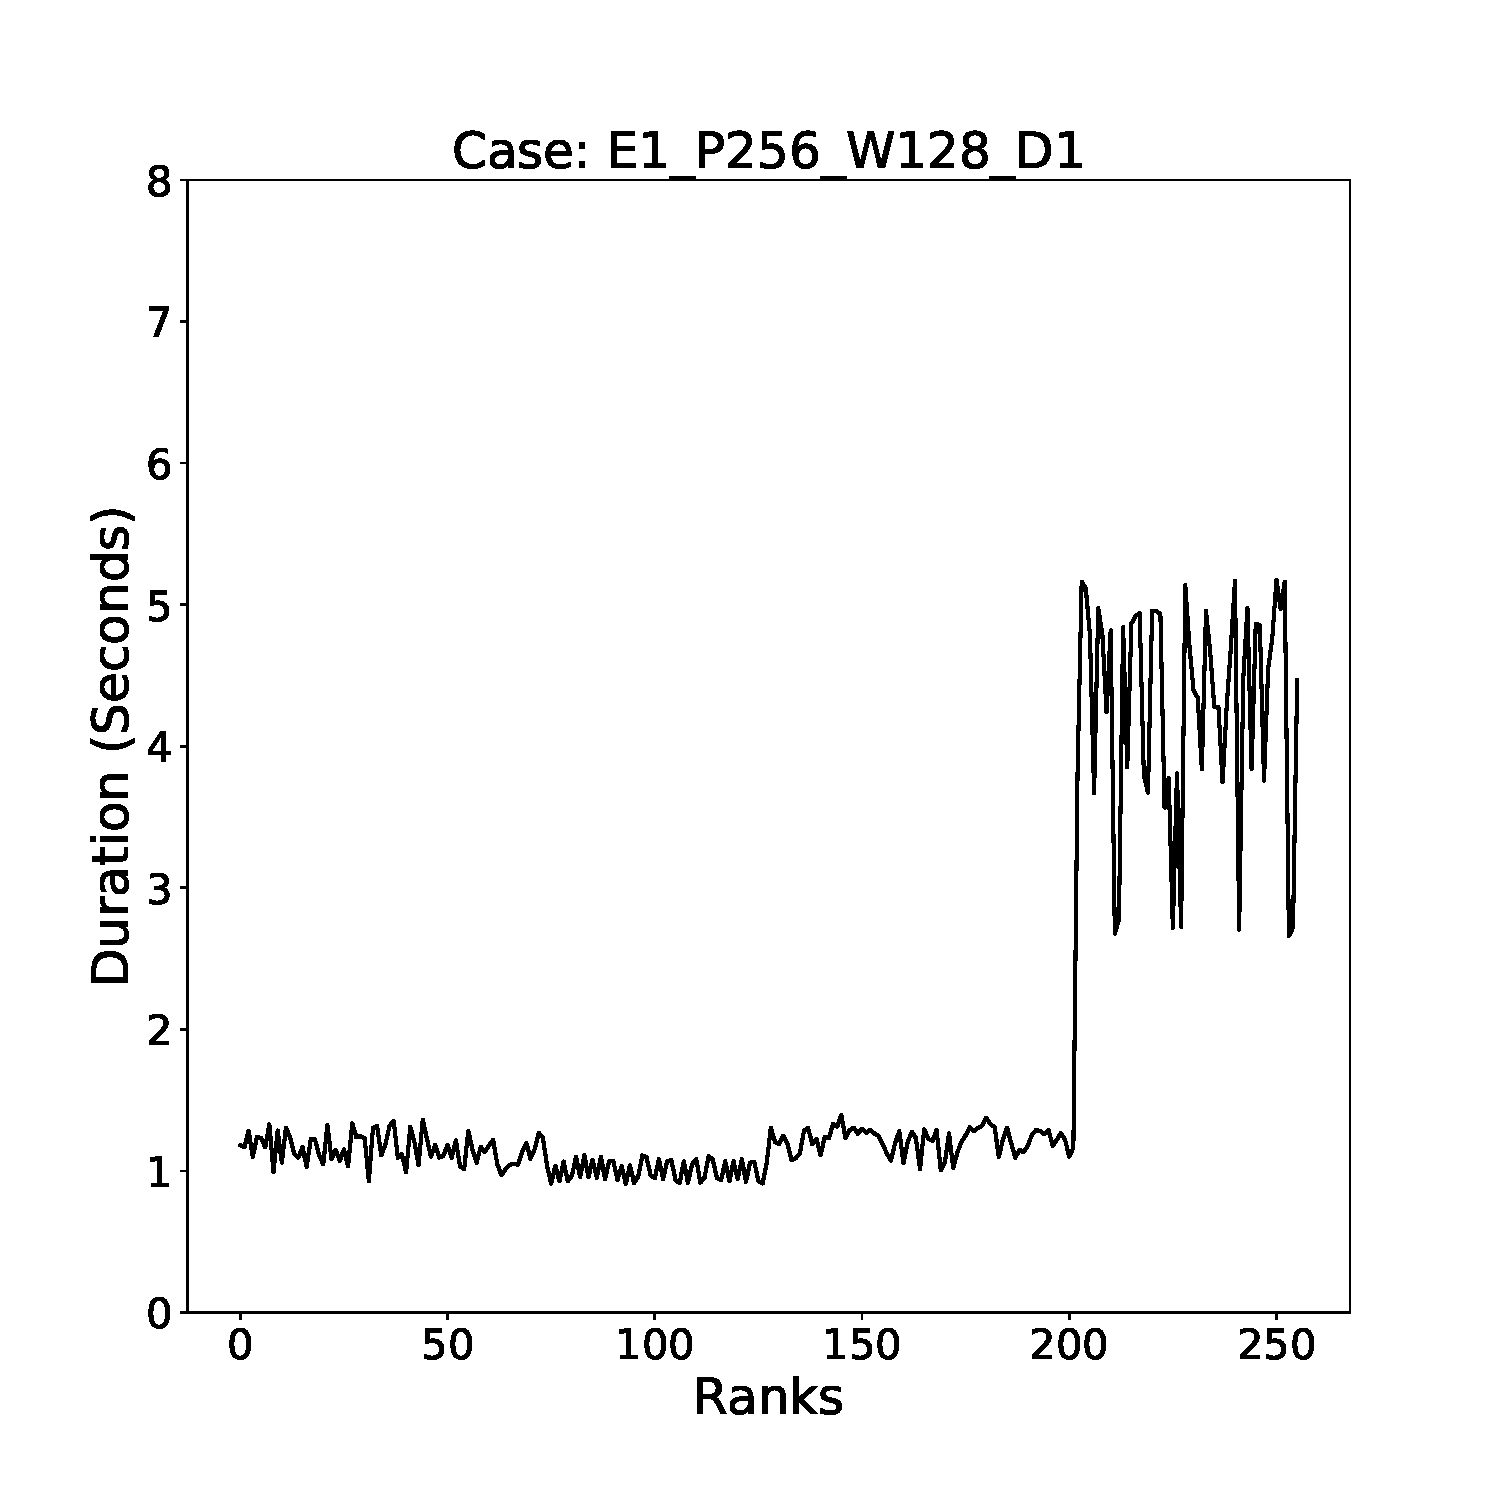
\includegraphics[width=\textwidth, height=\textwidth]{figures/E1_P256_W128_D1.pdf}
         \caption{Run\,1, 1\,GiB per process}
         \label{fig:E1_1}
     \end{subfigure}
     \hfill
     \begin{subfigure}[b]{0.3\textwidth}
         \centering
         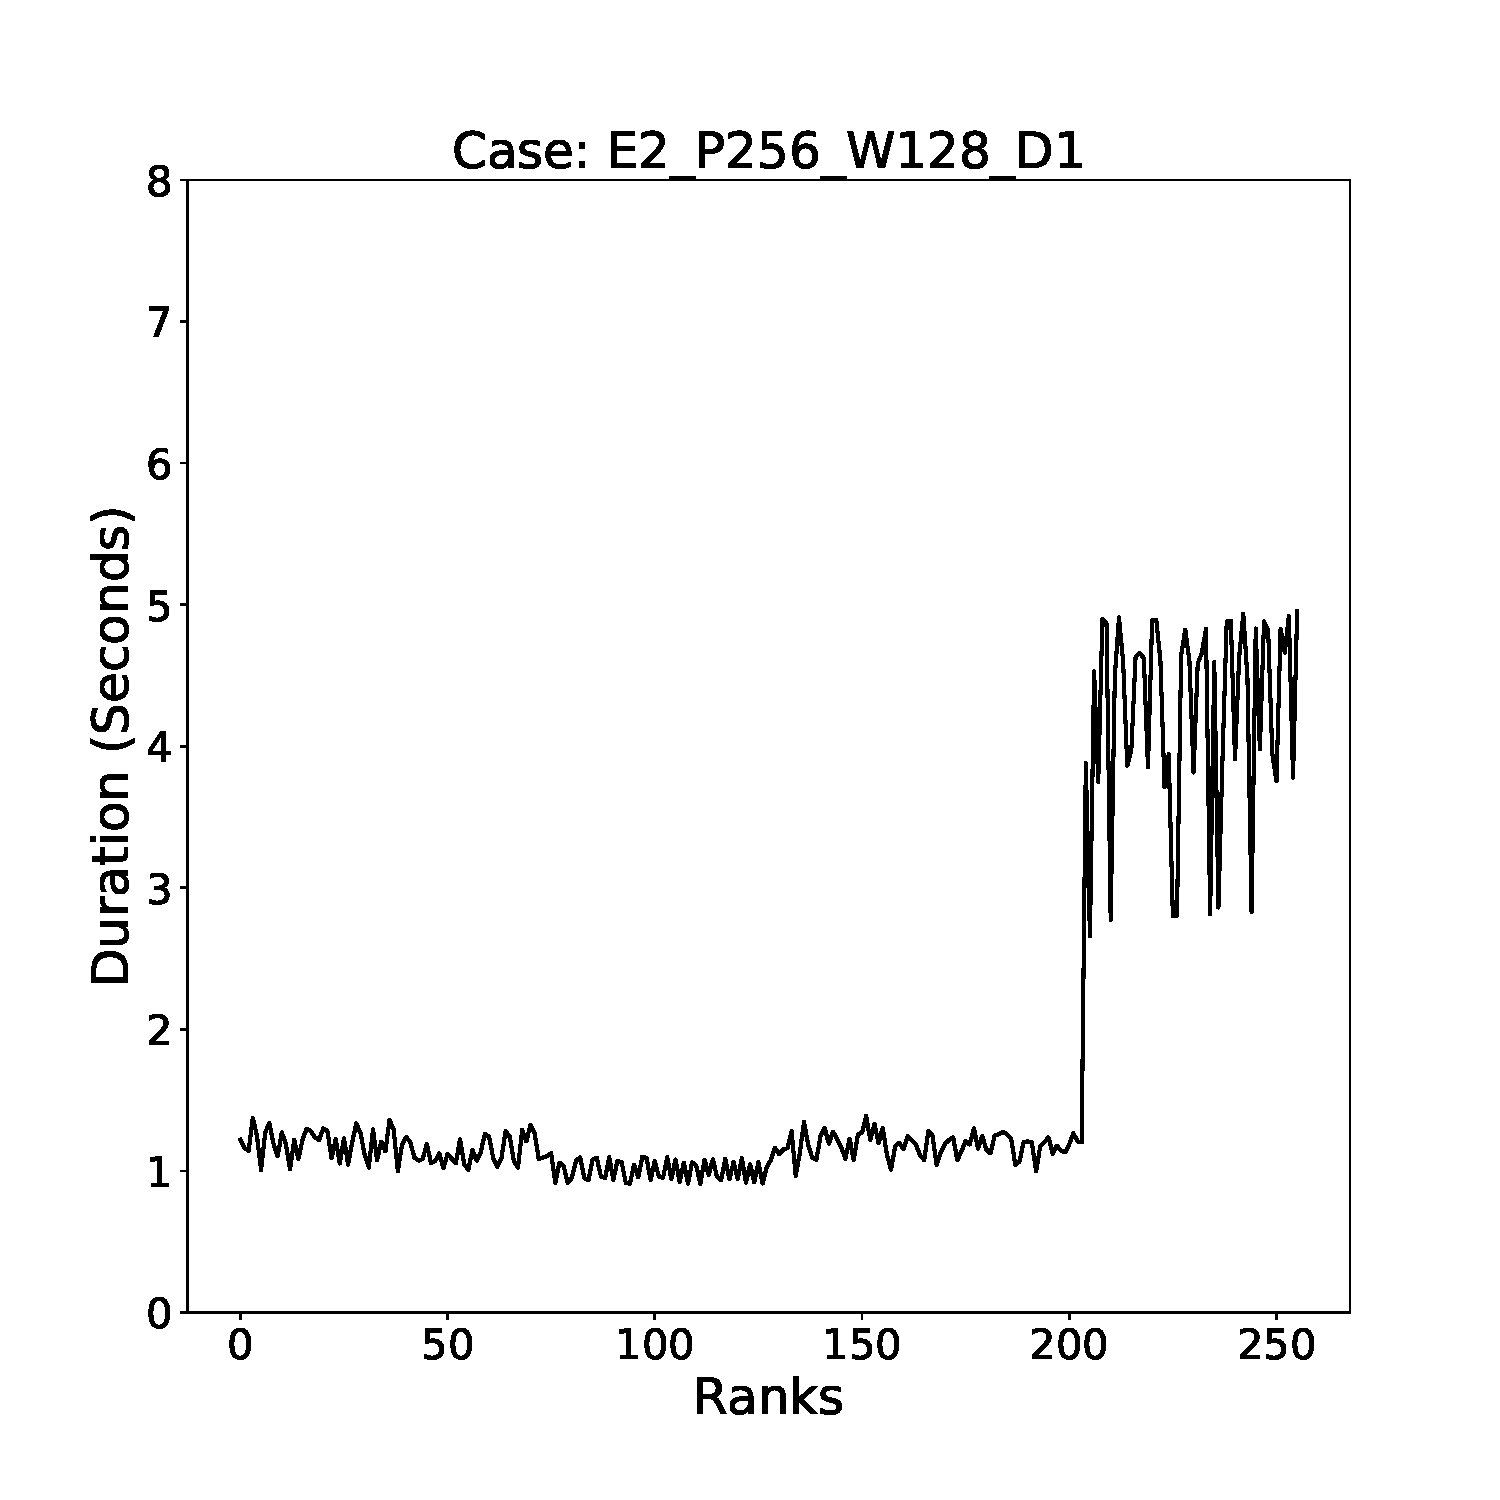
\includegraphics[width=\textwidth, height=\textwidth]{figures/E2_P256_W128_D1.pdf}
         \caption{Run\,2, 1\,GiB per process}
         \label{fig:E2_1}
     \end{subfigure}
      \hfill
     \begin{subfigure}[b]{0.3\textwidth}
         \centering
         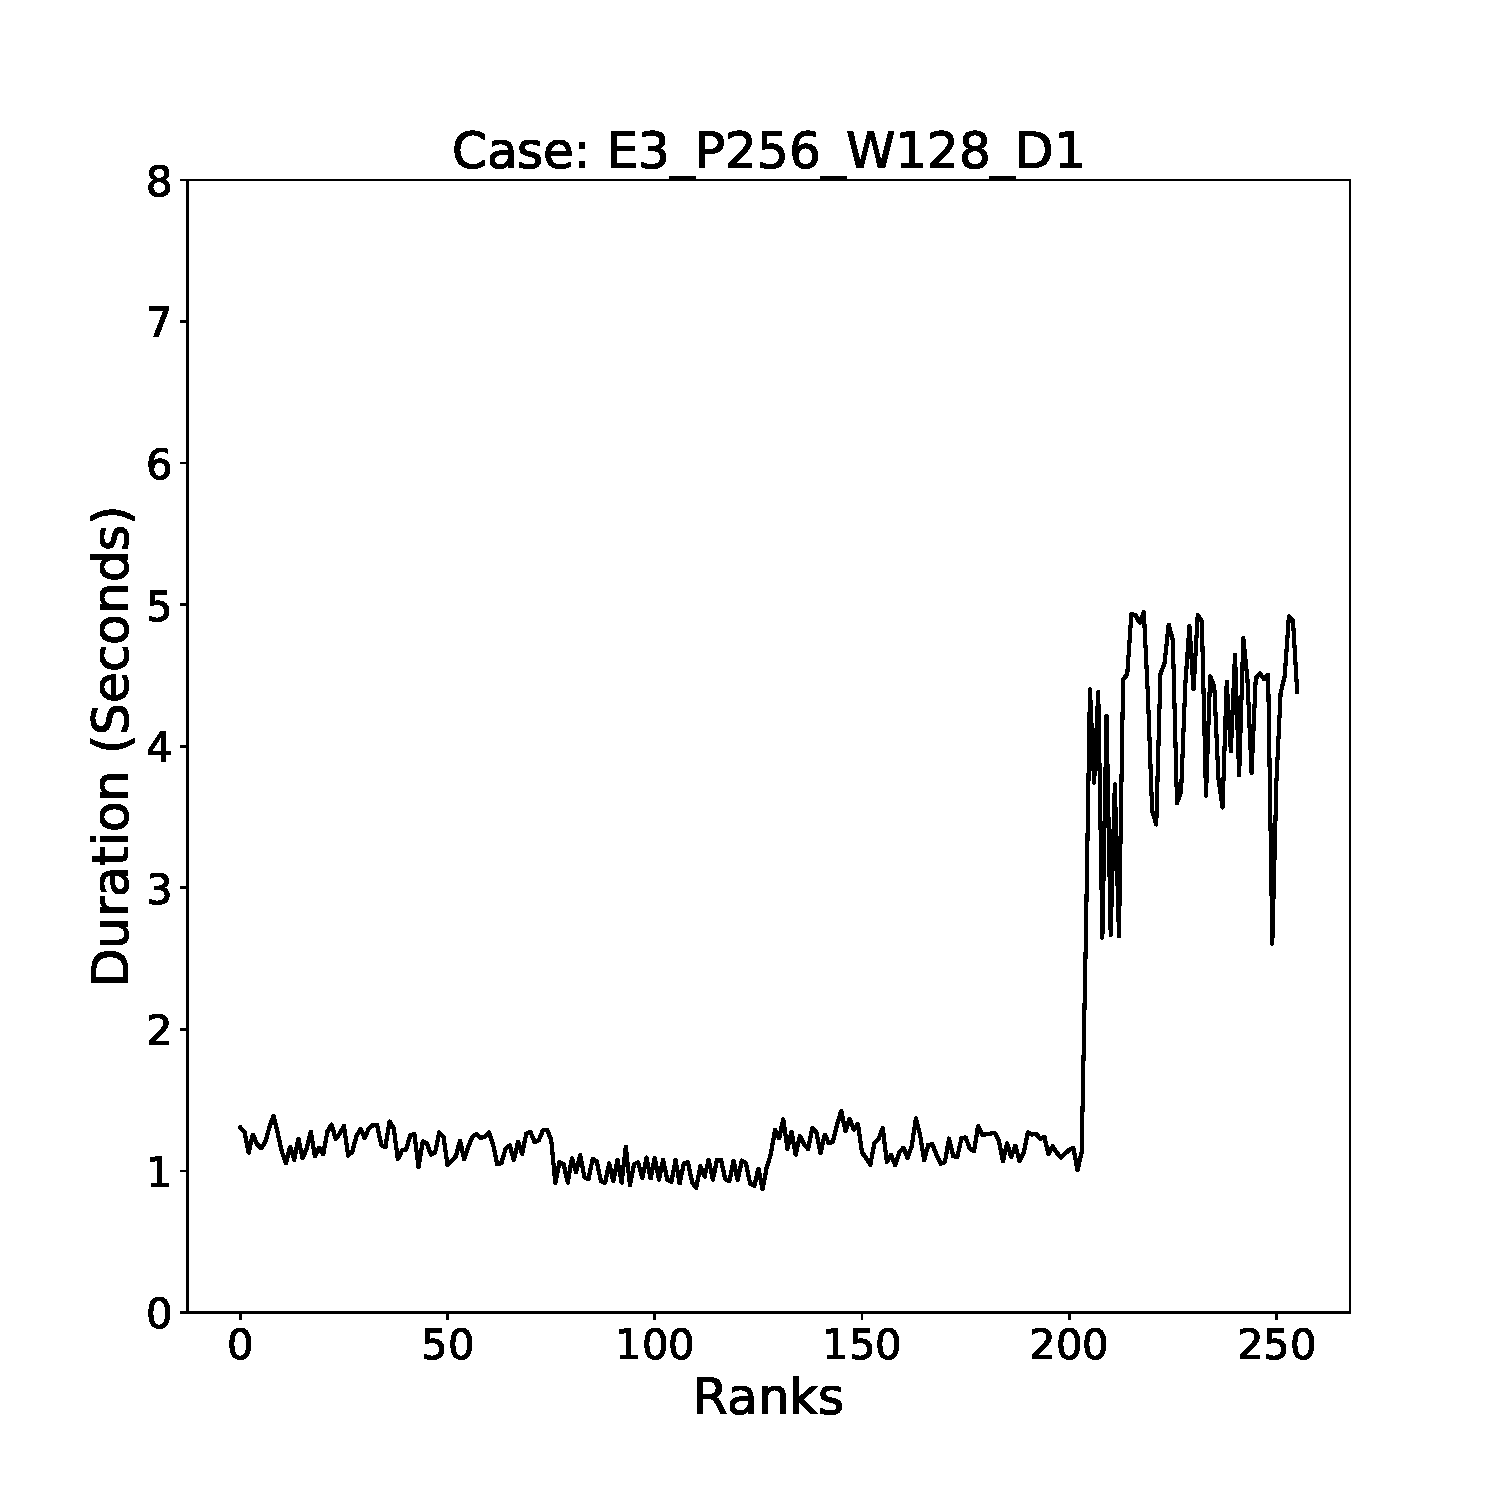
\includegraphics[width=\textwidth, height=\textwidth]{figures/E3_P256_W128_D1.pdf}
         \caption{Run\,3, 1\,GiB per process}
         \label{fig:E3_1}
     \end{subfigure}
        \caption{Average communication time for DEISA3 experiments, the number of processes is fixed to 256, we vary the size of the data from 128\,MiB to 1\,GiB, and we show results over the 3 runs.}
        \label{fig:variability}
\end{figure}


We were also interested in the behaviour of DEISA2 and DEISA1, the variability over ranks, iterations and runs, which we represent in Figure~\ref{fig:variability2} and Figure~\ref{fig:variability11} respectively.  
Our expectations are much more related to the variability over iterations, which will be more visible in DEISA1. 
Remember that in DEISA2, we have fixed the heartbeat interval of the bridges to one minute, and in DEISA1, we have kept the value by default which was 5 seconds. This frequency, alongside the frequent metadata sent to the scheduler, may cause more variability per iteration because of the load in the scheduler in DEISA1.  

Indeed the red band, which represents the standard deviation per iteration, is more visible in the DEISA1 experiments, less in DEISA2 and almost not visible in DEISA3. And this is thanks to the improvements over the three versions: less metadata and even fewer heartbeat messages coming from the bridges.
The takeaway from those experiments is that we could improve performance by minimizing the frequency of messages sent to the scheduler from the bridges. This does not affect the operation of \dask, because the role of the bridges is to send data to the workers only without submitting any tasks to the scheduler. Thus the scheduler does not need to know if they still need results as they even don't wait for any. 
The only variability that we still encounter is the one related to the placement of the process, scheduler and workers. 

\begin{figure}
     \centering
     \begin{subfigure}[b]{0.3\textwidth}
         \centering
         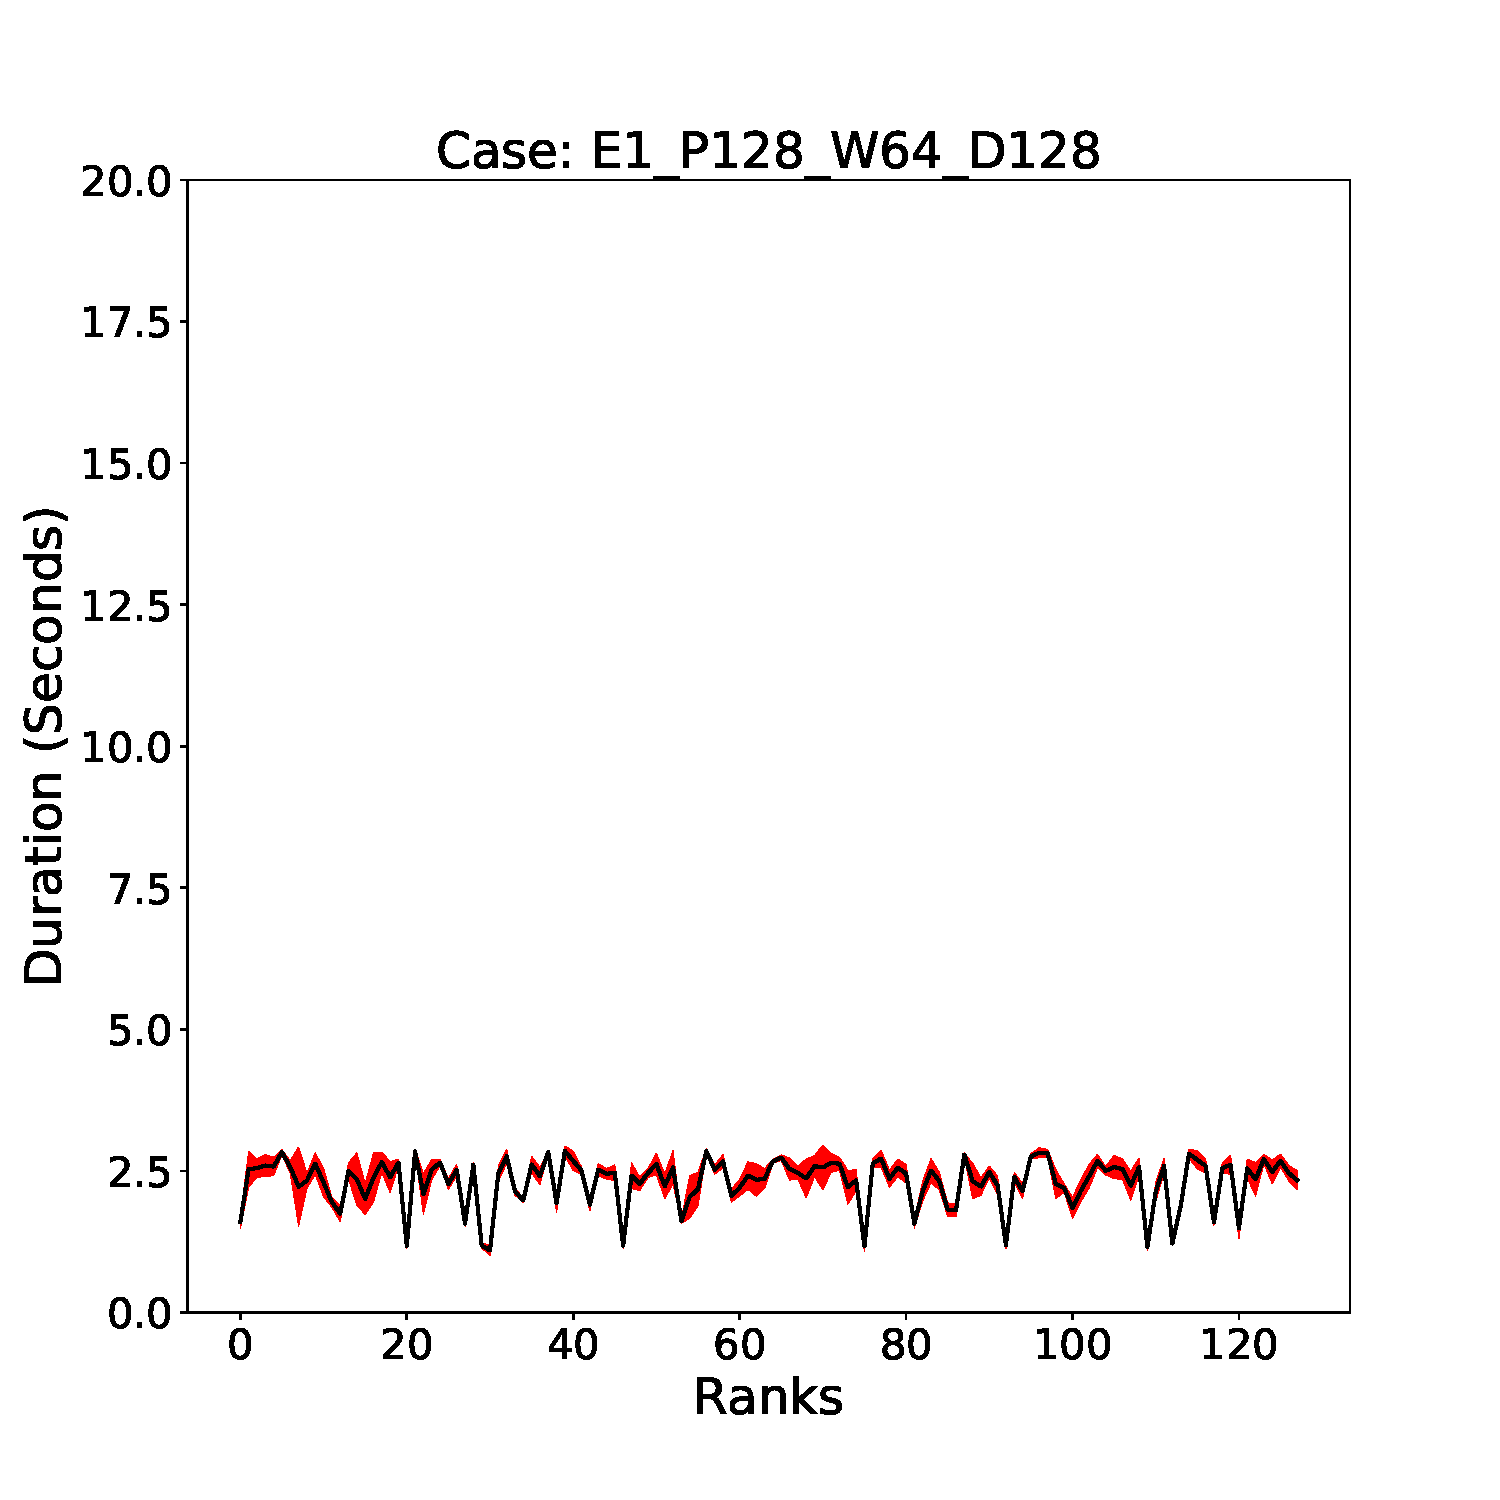
\includegraphics[width=\textwidth, height=\textwidth]{figures/deisa2__E1_P128_W64_D128.pdf}
         \caption{Run\,1, 128\,MiB per process}
         \label{fig:E1_128_d2}
     \end{subfigure}
     \hfill
     \begin{subfigure}[b]{0.3\textwidth}
         \centering
         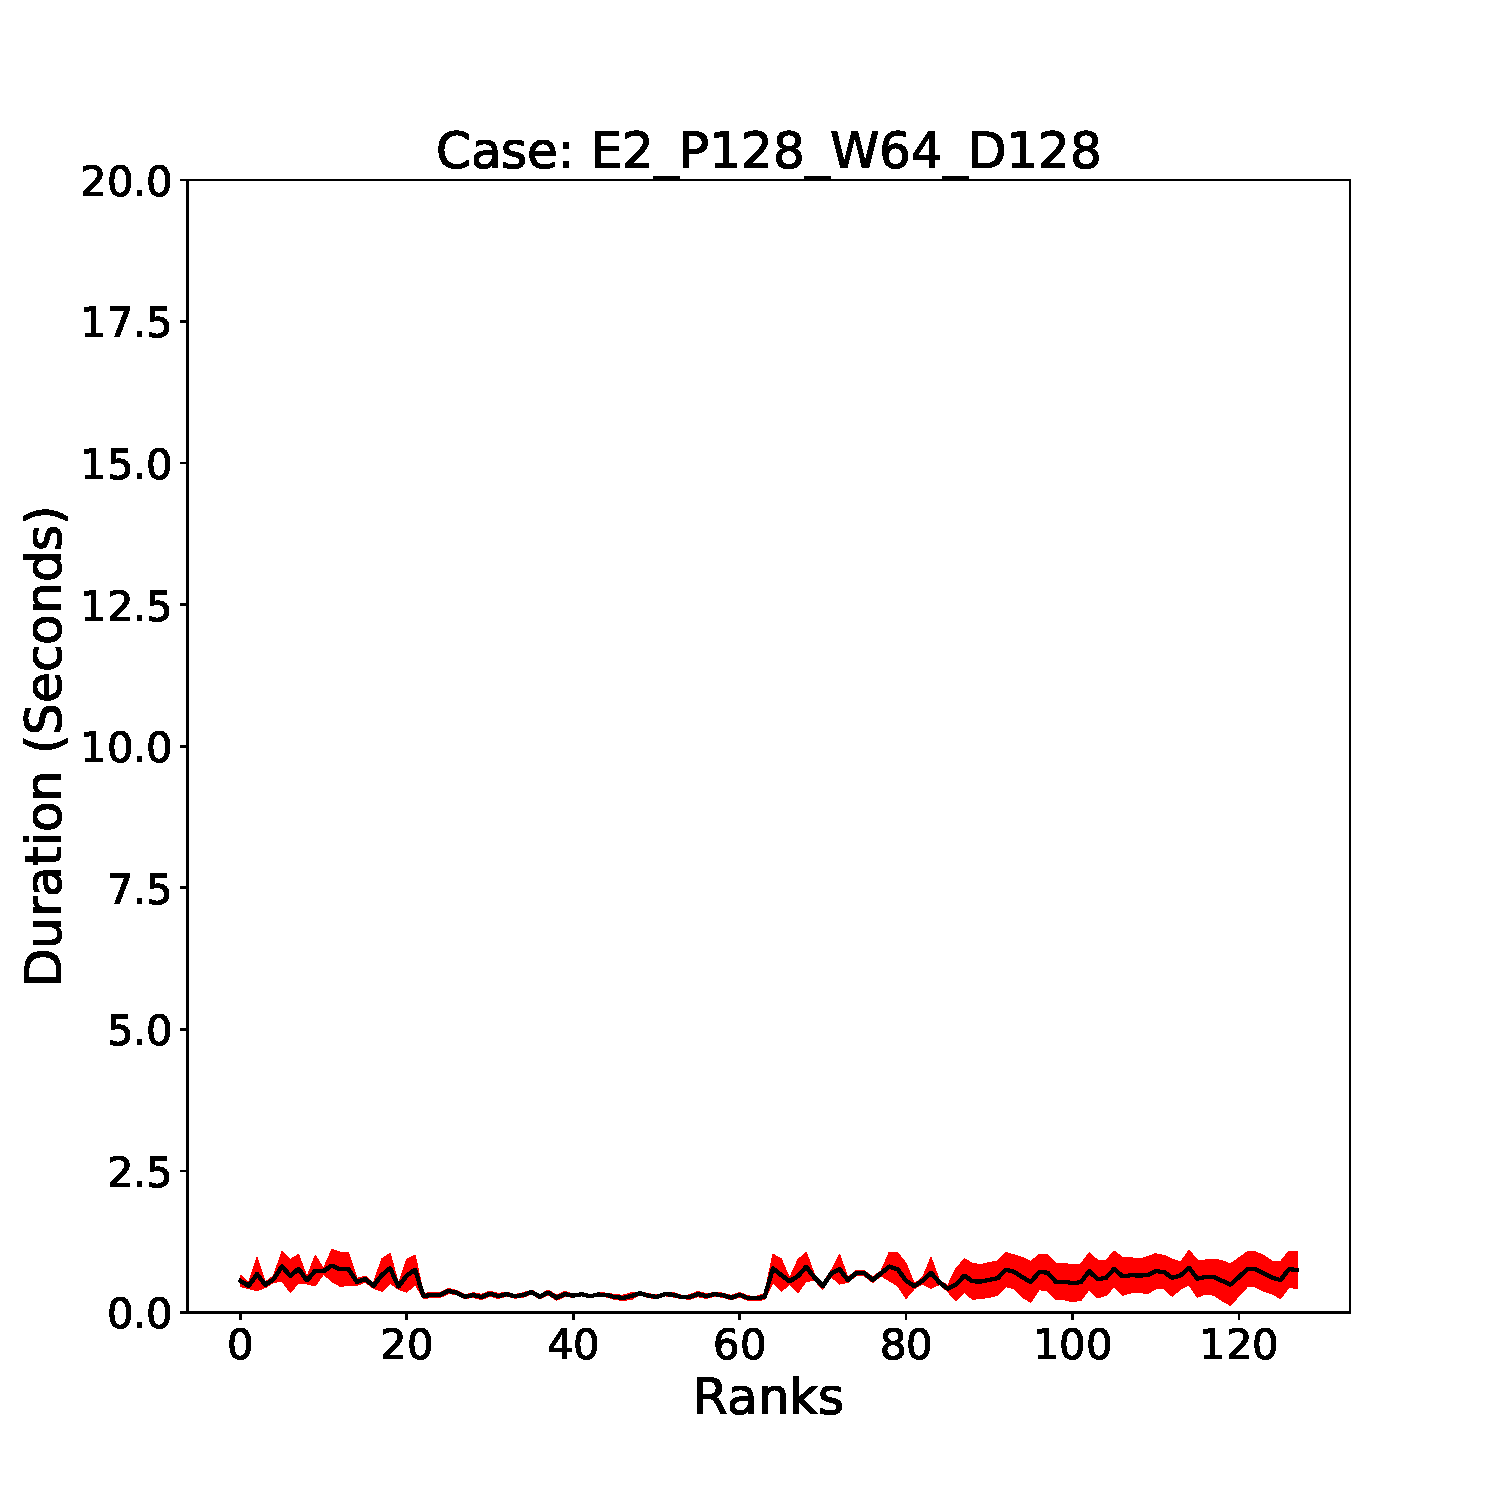
\includegraphics[width=\textwidth, height=\textwidth]{figures/deisa2__E2_P128_W64_D128.pdf}
         \caption{Run\,2, 128\,MiB per process}
         \label{fig:E2_128_d2}
     \end{subfigure}
      \hfill
     \begin{subfigure}[b]{0.3\textwidth}
         \centering
         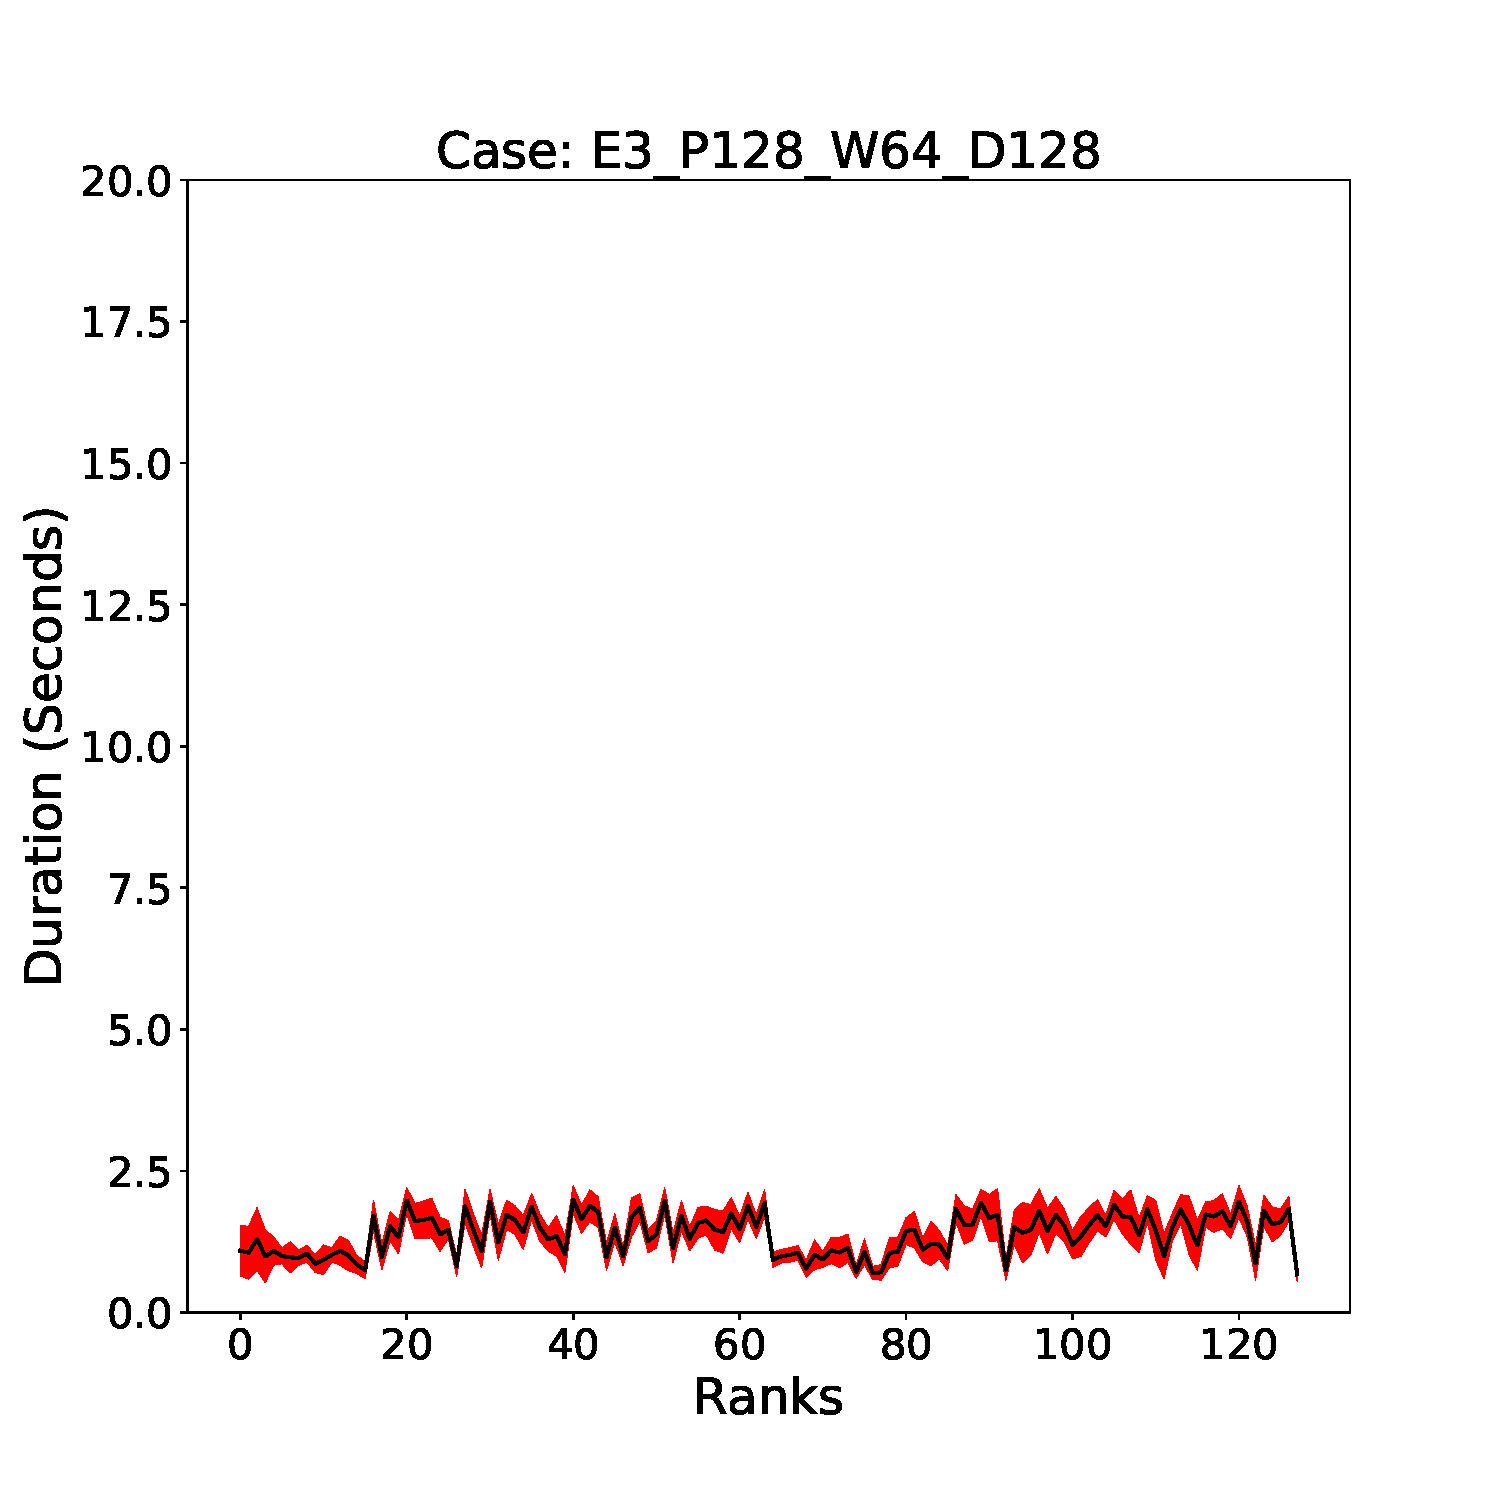
\includegraphics[width=\textwidth, height=\textwidth]{figures/deisa2__E3_P128_W64_D128.pdf}
         \caption{Run\,3, 128\,MiB per process}
         \label{fig:E3_128_d2}
     \end{subfigure}
     \vfill
     \begin{subfigure}[b]{0.3\textwidth}
         \centering
         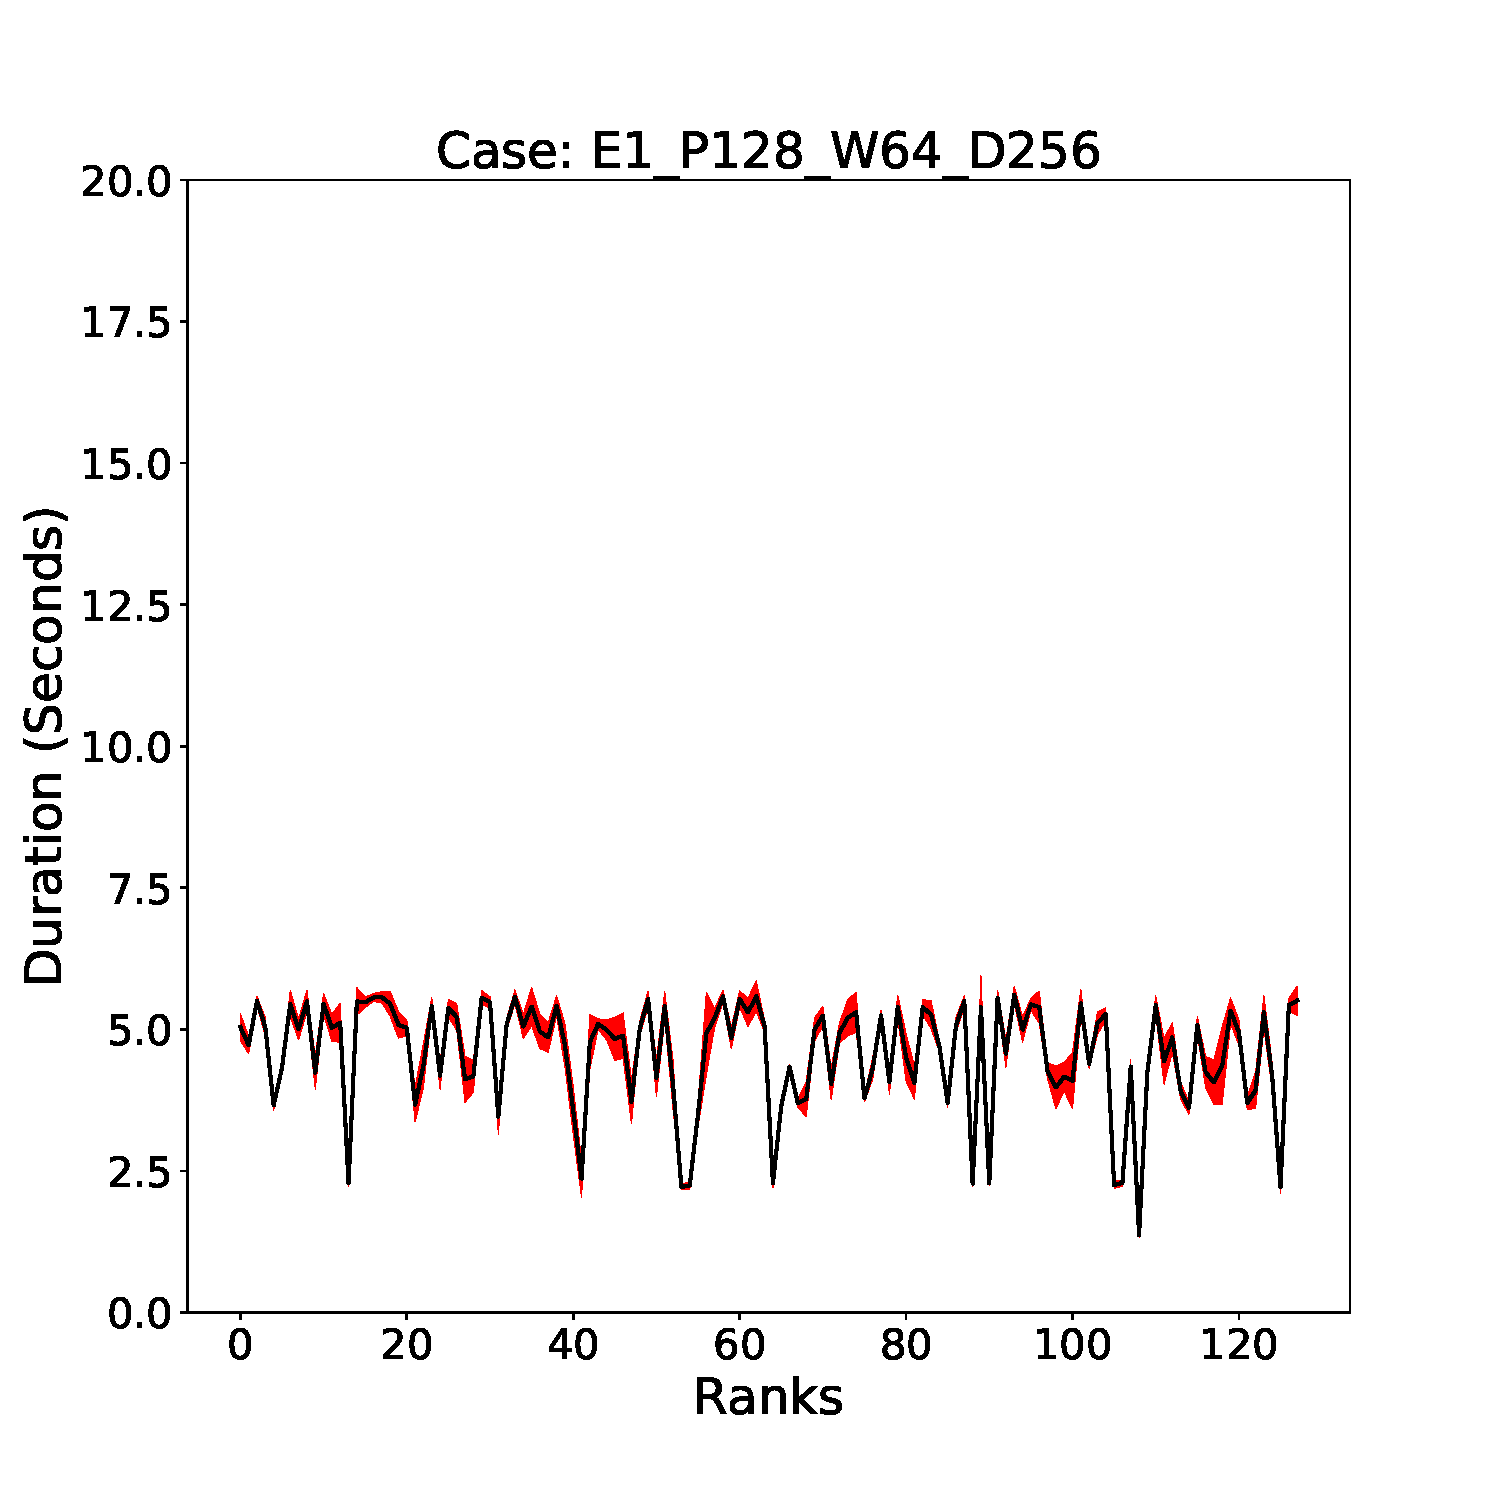
\includegraphics[width=\textwidth, height=\textwidth]{figures/deisa2__E1_P128_W64_D256.pdf}
         \caption{Run\,1, 256\,MiB per process }
         \label{fig:E1_256_d2}
     \end{subfigure}
     \hfill
     \begin{subfigure}[b]{0.3\textwidth}
         \centering
         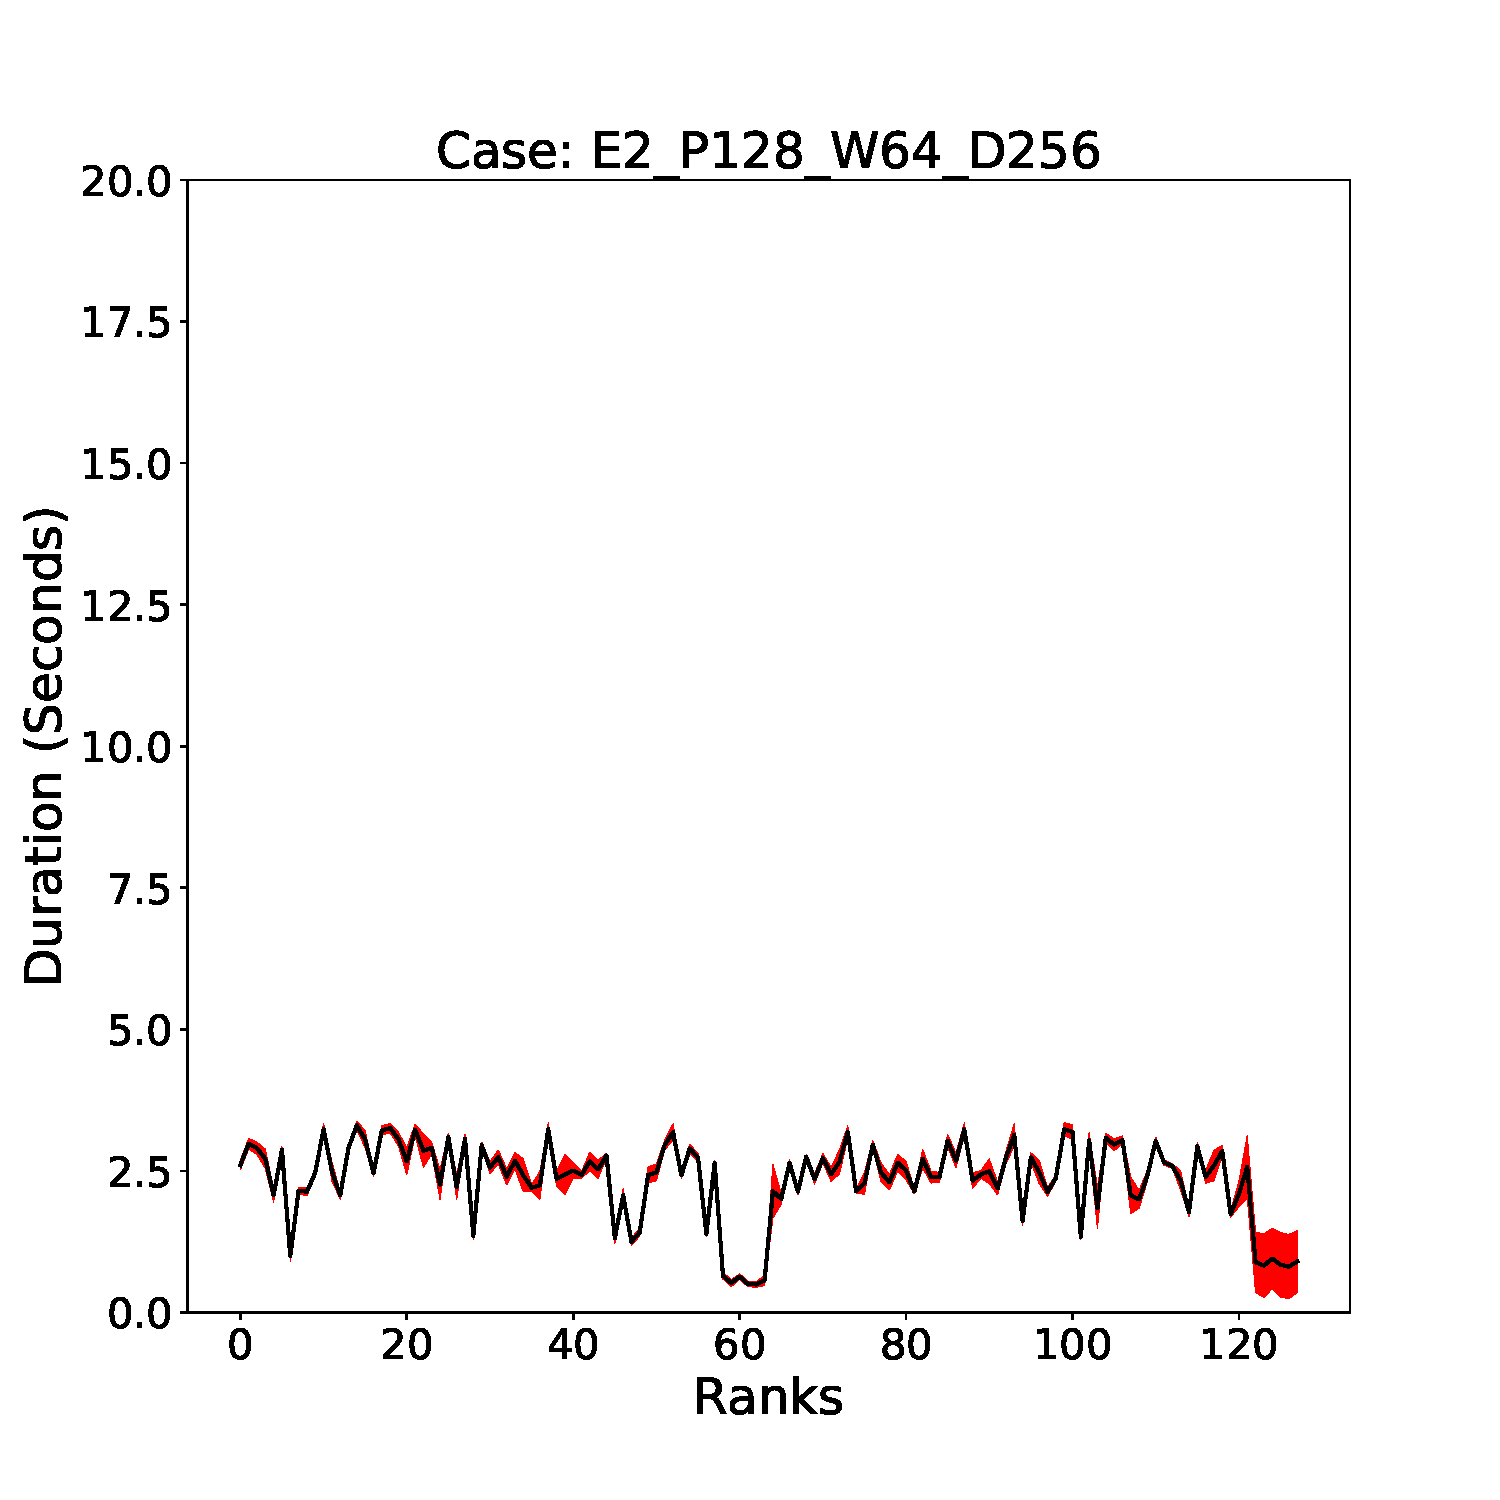
\includegraphics[width=\textwidth, height=\textwidth]{figures/deisa2__E2_P128_W64_D256.pdf}
         \caption{Run\,2, 256\,MiB per process}
         \label{fig:E2_256_d2}
     \end{subfigure}
      \hfill
     \begin{subfigure}[b]{0.3\textwidth}
         \centering
         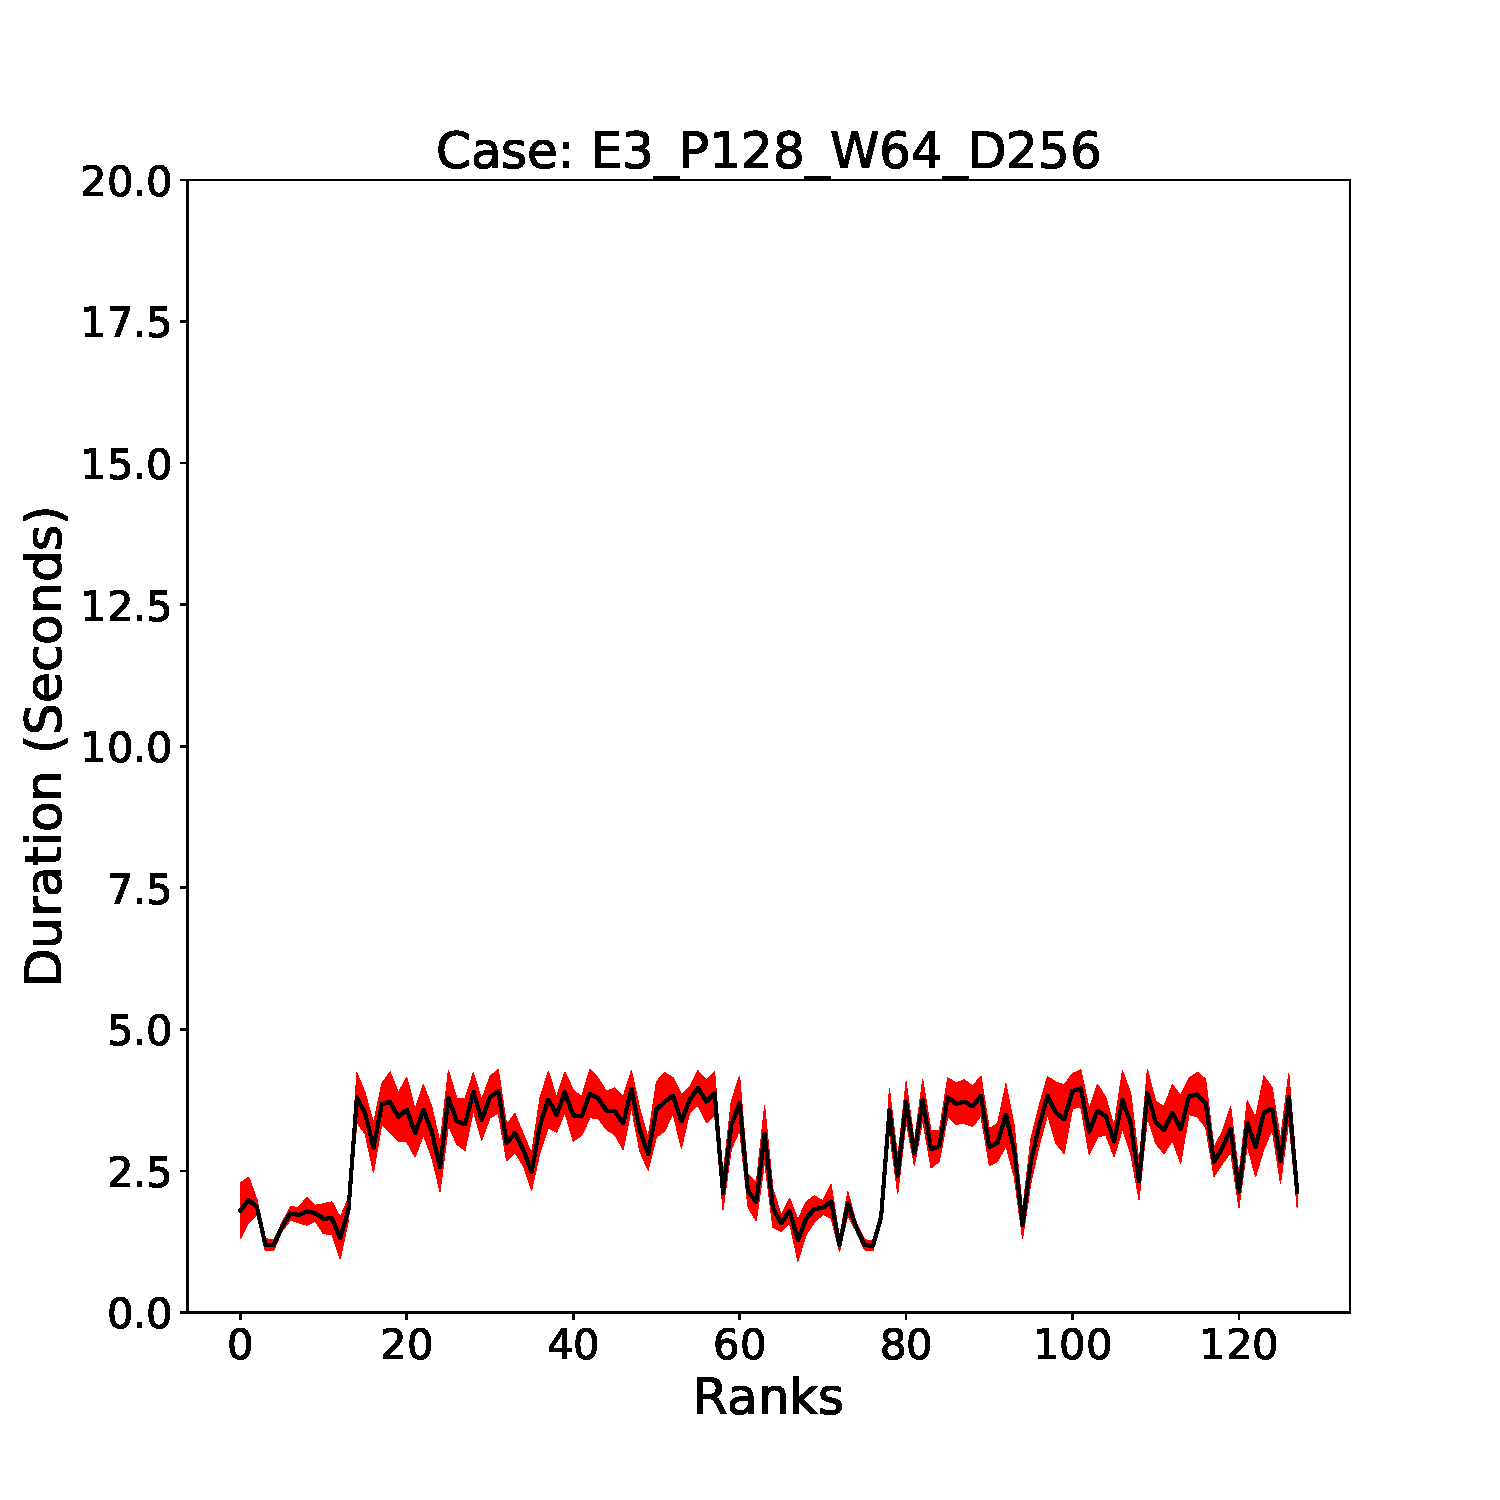
\includegraphics[width=\textwidth, height=\textwidth]{figures/deisa2__E3_P128_W64_D256.pdf}
         \caption{Run\,3, 256\,MiB per process}
         \label{fig:E3_256_d2}
     \end{subfigure}
     \vfill
          \begin{subfigure}[b]{0.3\textwidth}
         \centering
         \includegraphics[width=\textwidth, height=\textwidth]{figures/deisa2__E1_P128_W64_D512.pdf}
         \caption{Run\,1, 512\,MiB per process}
         \label{fig:E1_512_d2}
     \end{subfigure}
     \hfill
     \begin{subfigure}[b]{0.3\textwidth}
         \centering
         \includegraphics[width=\textwidth, height=\textwidth]{figures/deisa2__E2_P128_W64_D512.pdf}
         \caption{Run\,2, 512\,MiB per process}
         \label{fig:E2_512_d2}
     \end{subfigure}
      \hfill
     \begin{subfigure}[b]{0.3\textwidth}
         \centering
         \includegraphics[width=\textwidth, height=\textwidth]{figures/deisa2__E3_P128_W64_D512.pdf}
         \caption{Run\,3, 512\,MiB per process}
         \label{fig:E3_512_d2}
     \end{subfigure}
     \vfill
          \begin{subfigure}[b]{0.3\textwidth}
         \centering
         \includegraphics[width=\textwidth, height=\textwidth]{figures/deisa2__E1_P128_W64_D1.pdf}
         \caption{Run\,1, 1\,GiB per process}
         \label{fig:E1_1_d2}
     \end{subfigure}
     \hfill
     \begin{subfigure}[b]{0.3\textwidth}
         \centering
         \includegraphics[width=\textwidth, height=\textwidth]{figures/deisa2__E2_P128_W64_D1.pdf}
         \caption{Run\,2, 1\,GiB per process}
         \label{fig:E2_1_d2}
     \end{subfigure}
      \hfill
     \begin{subfigure}[b]{0.3\textwidth}
         \centering
         \includegraphics[width=\textwidth, height=\textwidth]{figures/deisa2__E3_P128_W64_D1.pdf}
         \caption{Run\,3, 1\,GiB per process}
         \label{fig:E3_1_d2}
     \end{subfigure}
        \caption{Average communication time for DEISA2 experiments, the number of processes is fixed to 128, we vary the size of the data from 128\,MiB to 1\,GiB, and we show results over the 3 runs.}
        \label{fig:variability2}
\end{figure}


\begin{figure}
     \centering
     \begin{subfigure}[b]{0.3\textwidth}
         \centering
         \includegraphics[width=\textwidth, height=\textwidth]{figures/deisa1__E1_P128_W64_D128.pdf}
         \caption{Run\,1, 128\,MiB per process}
         \label{fig:E1_128_d11}
     \end{subfigure}
     \hfill
     \begin{subfigure}[b]{0.3\textwidth}
         \centering
         \includegraphics[width=\textwidth, height=\textwidth]{figures/deisa1__E2_P128_W64_D128.pdf}
         \caption{Run\,2, 128\,MiB per process}
         \label{fig:E2_128_d11}
     \end{subfigure}
      \hfill
     \begin{subfigure}[b]{0.3\textwidth}
         \centering
         \includegraphics[width=\textwidth, height=\textwidth]{figures/deisa1__E3_P128_W64_D128.pdf}
         \caption{Run\,3, 128\,MiB per process}
         \label{fig:E3_128_d11}
     \end{subfigure}
     \vfill
     \begin{subfigure}[b]{0.3\textwidth}
         \centering
         \includegraphics[width=\textwidth, height=\textwidth]{figures/deisa1__E1_P128_W64_D256.pdf}
         \caption{Run\,1, 256\,MiB per process }
         \label{fig:E1_256_d11}
     \end{subfigure}
     \hfill
     \begin{subfigure}[b]{0.3\textwidth}
         \centering
         \includegraphics[width=\textwidth, height=\textwidth]{figures/deisa1__E2_P128_W64_D256.pdf}
         \caption{Run\,2, 256\,MiB per process}
         \label{fig:E2_256_d11}
     \end{subfigure}
      \hfill
     \begin{subfigure}[b]{0.3\textwidth}
         \centering
         \includegraphics[width=\textwidth, height=\textwidth]{figures/deisa1__E3_P128_W64_D256.pdf}
         \caption{Run\,3, 256\,MiB per process}
         \label{fig:E3_256_d11}
     \end{subfigure}
     \vfill
          \begin{subfigure}[b]{0.3\textwidth}
         \centering
         \includegraphics[width=\textwidth, height=\textwidth]{figures/deisa1__E1_P128_W64_D512.pdf}
         \caption{Run\,1, 512\,MiB per process}
         \label{fig:E1_512_d11}
     \end{subfigure}
     \hfill
     \begin{subfigure}[b]{0.3\textwidth}
         \centering
         \includegraphics[width=\textwidth, height=\textwidth]{figures/deisa1__E2_P128_W64_D512.pdf}
         \caption{Run\,2, 512\,MiB per process}
         \label{fig:E2_512_d11}
     \end{subfigure}
      \hfill
     \begin{subfigure}[b]{0.3\textwidth}
         \centering
         \includegraphics[width=\textwidth, height=\textwidth]{figures/deisa1__E3_P128_W64_D512.pdf}
         \caption{Run\,3, 512\,MiB per process}
         \label{fig:E3_512_d11}
     \end{subfigure}
     \vfill
          \begin{subfigure}[b]{0.3\textwidth}
         \centering
         \includegraphics[width=\textwidth, height=\textwidth]{figures/deisa1__E1_P128_W64_D1.pdf}
         \caption{Run\,1, 1\,GiB per process}
         \label{fig:E1_1_d11}
     \end{subfigure}
     \hfill
     \begin{subfigure}[b]{0.3\textwidth}
         \centering
         \includegraphics[width=\textwidth, height=\textwidth]{figures/deisa1__E2_P128_W64_D1.pdf}
         \caption{Run\,2, 1\,GiB per process}
         \label{fig:E2_1_d11}
     \end{subfigure}
      \hfill
     \begin{subfigure}[b]{0.3\textwidth}
         \centering
         \includegraphics[width=\textwidth, height=\textwidth]{figures/deisa1__E3_P128_W64_D1.pdf}
         \caption{Run\,3, 1\,GiB per process}
         \label{fig:E3_1_d11}
     \end{subfigure}
        \caption{Average communication time for DEISA1 experiments, the number of processes is fixed to 128, we vary the size of the data from 128\,MiB to 1\,GiB, and we show results over the 3 runs.}
        \label{fig:variability11}
\end{figure}



\begin{figure}
     \centering
     \begin{subfigure}[b]{0.3\textwidth}
         \centering
         \includegraphics[width=\textwidth, height=\textwidth]{figures/deisa2__E1_P64_W32_D1.pdf}
         \caption{Run\,1, 1\,GiB per process}
         \label{fig:E1_1_d22}
     \end{subfigure}
     \hfill
     \begin{subfigure}[b]{0.3\textwidth}
         \centering
         \includegraphics[width=\textwidth, height=\textwidth]{figures/deisa2__E2_P64_W32_D1.pdf}
         \caption{Run\,2, 1\,GiB per process}
         \label{fig:E2_1_d22}
     \end{subfigure}
      \hfill
     \begin{subfigure}[b]{0.3\textwidth}
         \centering
         \includegraphics[width=\textwidth, height=\textwidth]{figures/deisa2__E3_P64_W32_D1.pdf}
         \caption{Run\,3, 1\,GiB per process}
         \label{fig:E3_1_d22}
     \end{subfigure}
        \caption{Average communication time for DEISA2 experiments, the number of processes is fixed to 64 and the size of the data to 1\,GiB, and we show results over the 3 runs.}
        \label{fig:variability222}
\end{figure}


In this last part, we are interested in the strange values we got in Figure~\ref{fig:perfX2}.
In Figure~\ref{fig:variability222}, the number of processes is 64, and the data size is 1\,GiB for DEISA2. We notice that there is a big variability over processes and runs and a small one over iterations. In best cases, we spend 2 seconds to send the data, and in the worst cases, we spend around 12 seconds.  
In Figure~\ref{fig:variability3}, the number of processes is 128, and the data size is 1\,GiB for DEISA3. We notice that there is variability over ranks and runs but not over iterations (we do not notice the red band of the standard deviation over iterations). In best cases, we spend around 1 second to send the 1\,GiB; in worst ones, we spend more than 10 seconds.
For both cases, since we take the maximal value registered by all the ranks before we compute the mean over iterations and runs in Figure~\ref{fig:perfX2}, we likely capture the worst cases. 

\begin{figure}
     \centering
    \begin{subfigure}[b]{0.3\textwidth}
         \centering
         \includegraphics[width=\textwidth, height=\textwidth]{figures/E1_P128_W64_D1.pdf}
         \caption{Run\,1, 1\,GiB per process}
         \label{fig:E1_1_d3}
     \end{subfigure}
     \hfill
     \begin{subfigure}[b]{0.3\textwidth}
         \centering
         \includegraphics[width=\textwidth, height=\textwidth]{figures/E2_P128_W64_D1.pdf}
         \caption{Run\,2, 1\,GiB per process}
         \label{fig:E2_1_d3}
     \end{subfigure}
      \hfill
     \begin{subfigure}[b]{0.3\textwidth}
         \centering
         \includegraphics[width=\textwidth, height=\textwidth]{figures/E3_P128_W64_D1.pdf}
         \caption{Run\,3, 1\,GiB per process}
         \label{fig:E3_1_d3}
     \end{subfigure}
        \caption{Average communication time for DEISA3 experiments, the number of processes is fixed to 128 and the size is 1\,GiB, and we show results over the 3 runs.}
        \label{fig:variability3}
\end{figure}


We did not do further investigation on that. However, we can consider optimizing communications with the placement of the workers and simulation processes as a perspective.

\subsubsection{Experiment IV}\label{XP4}
%isipca vs ipca for post vs isipca deisa v3 : perf plus interface 
In this section, we will analyse the performance of the new version of \deisa (DEISA3) compared to the old version (DEISA1) with post hoc performance using \dask. We will compare the results of the IPCA we had in the previous chapter to the results we got with the new version of IPCA presented in Section~\ref{IPCA}. 

\begin{figure}
     \centering
     \begin{subfigure}[b]{0.3\textwidth}
         \centering
         \includegraphics[width=\textwidth, height=\textwidth]{figures/128MB_1vs3vspost1vspost2.pdf}
         \caption{Average simulation, communication and IO times per iteration for 128\,MiB per process}
         \label{fig:X1128_1_3_p}
     \end{subfigure}
     \hfill
     \begin{subfigure}[b]{0.3\textwidth}
         \centering
         \includegraphics[width=\textwidth, height=\textwidth]{figures/256MB_1vs3vspost1vspost2.pdf}
         \caption{Average simulation, communication and IO times per iteration for 256\,MiB per process}
         \label{fig:X256_1_3_p}
     \end{subfigure}
     \hfill
     \begin{subfigure}[b]{0.3\textwidth}
         \centering
         \includegraphics[width=\textwidth, height=\textwidth]{figures/512MB_1vs3vspost1vspost2.pdf}
         \caption{Average simulation, communication and IO times per iteration for 512\,MiB per process}
         \label{fig:X512_1_3_p}
     \end{subfigure}
        \caption{Weak scaling average simulation, communication and IO times per iteration for 128\,MiB, 256\,MiB and 512\,MiB per process for three experiments: the first stacked bar from the left of each scale represent results for post hoc version: simulation in green, communications in red. The second stacked bar shows results for the old version of \deisa (DEISA1): simulation in green and communication in pink. The third stacked bar shows results for the new version of \deisa (DEISA3): the simulation in green and the communications in violet.}
        \label{fig:perfX4}
\end{figure}

Figure~\ref{fig:perfX4} summarizes weak scaling performance from the simulation side. The first subfigure from the left shows results for 128\,MiB per process, in the middle for 256\,MiB and the right for 512\,MiB. 
The x-axis represents the processes, and the y-axis shows the mean duration over runs and the iteration of the maximum duration over ranks. The error bar represents the standard deviation. We have noticed that the first iteration of the post hoc version was longer than the others. We expect that it is due to file creation. We have only computed the mean and the standard deviation over the nine iterations. 

The different results in those subfigures were already discussed in the previous sections. The HDF5 writes are chunked, so we have almost the same HDF5 write time.
The communication times for both \deisa versions are almost similar, with more variability in DEISA1.  
The missed values for post hoc here are due to crashes in the simulation side, likely because of the bug in HDF5~\cite{large_2023}.

\begin{figure}
     \centering
     \begin{subfigure}[b]{0.3\textwidth}
         \centering
         \includegraphics[width=\textwidth, height=\textwidth]{figures/128A_1vs3vspost1vspost2.pdf}
         \caption{Average analytics duration for 128\,MiB chunk size }
         \label{fig:A1128_1_3_p}
     \end{subfigure}
     \hfill
     \begin{subfigure}[b]{0.3\textwidth}
         \centering
         \includegraphics[width=\textwidth, height=\textwidth]{figures/256A_1vs3vspost1vspost2.pdf}
         \caption{Average analytics duration for 256\,MiB chunk size}
         \label{fig:A256_1_3_p}
     \end{subfigure}
     \hfill
     \begin{subfigure}[b]{0.3\textwidth}
         \centering
         \includegraphics[width=\textwidth, height=\textwidth]{figures/512A_1vs3vspost1vspost2.pdf}
         \caption{Average analytics duration for 512\,MiB chunk size}
         \label{fig:A512_1_3_p}
     \end{subfigure}
        \caption{Weak scaling average analytics time for 128\,MiB, 256\,MiB and 512\,MiB per process for three experiments: the first bar from the left of each scale (in red) represents analytics time for post hoc with the IPCA presented in Section~\ref{IPCA}. The second bar from the left (in orange) shows analytics time for the post hoc version with the new version of IPCA presented in Section~\ref{ISIPCA}. The third bar from the left (in violet) shows analytics time for the old version of \deisa (DEISA1) with the old IPCa, and the last bar from the left (purple) shows results for the new version of \deisa (DEISA3) with the new IPCA}. 
        \label{fig:perfA3}
\end{figure}

We will focus more on the analytics part to analyse how the two versions of IPCA performed. Figure~\ref{fig:perfA3} shows the weak scaling results for the analytics part of the different configurations of Experiment IV\ref{XP4}.
the first bar from the left of each scale (in red) represents analytics time for post hoc with the IPCA presented in Section~\ref{IPCA}. 
The second bar from the left (in orange) shows analytics time for the post hoc version with the new version of IPCA presented in Section~\ref{ISIPCA}. 
The third bar from the left (in violet) shows analytics time for the old version of \deisa (DEISA1), and the last bar from the left (purple) shows results for the new version of \deisa (DEISA3)
The x-axis of each subfigure represents the variation of the \dask workers from 2 to 32. The y-axis represents the duration in seconds of the analytics. 
The \deisa analytics time includes compute time and waiting for the data from the next step. The post hoc time includes reading the data from the disk and analysing the data. We have chunked the HDF5 files and used the same chunking in the analytics.
The represented values are the mean duration over the three runs. The bar errors are the standard deviation.      

For the different chunk sizes, for small scales, \deisa versions are comparable to post hoc versions. Post hoc with our new IPCA is even a bit more efficient than \deisa when the number of \dask workers is two. When increasing the problem size, \deisa versions perform better than post hoc, and we have already discussed that in the previous experiments. 

Our new version of IPCA scales better than the old version, both in post hoc and in situ experiments. for post hoc cases the new IPCA version is almost x1.8 faster when the chunk size is 256\,MiB, and the number of workers is 16. We expect that this is due to the way we submit tasks to \dask in the version of IPCA.
Instead of submitting the tasks for each \texttt{partial\_fit}, in the new version of the IPCA, we just create the underlying graph of the \texttt{partial\_fit} for each iteration and submit one task graph to \dask at the end. Doing so will let \dask optimize the execution of all the tasks over iterations and ovoids repetitive and unnecessary computations. For instance, if a given data is needed by two tasks submitted in two separate task graphs, \dask will perform two disk accesses, one for each submission. However, if those two tasks are in the same task graph, the data will be read only once and used by all the tasks present in the graph needing it. This is only one example, and \dask may perform more optimizations.    

This is also beneficial for in situ analytics (in DEISA1, we have used the old version, and in DEISA3, the new one). However, it is less visible as the waiting time for the simulation data is included, and the time to run tasks in in situ is usually short compared to reading data from disk. 


\begin{figure}[t]\centering
\includegraphics[width=\columnwidth]{figures/P64_W32_D128_DASK_ISIPCA.pdf}
\caption{Task stream generated by \dask for post hoc the new IPCA with chunking activated for 64 processes, 32 workers and 128\,MiB per process. 
    Number of tasks: 9693
    Compute time: 8359.85s
    Deserialize time: 26.64 s
    Disk-read time: 67.34 ms
    Transfer time: 1446.00 s
}
\label{fig:taskstreamdask3}
\end{figure}


\begin{figure}[t]\centering
\includegraphics[width=\columnwidth]{figures/P64_W32_D128_DEISA3_IPCA.pdf}
\caption{Task stream generated by \dask with in situ analytics enabled for the new IPCA, for 64 processes, 32 workers and 128\,MiB per process.
    Number of tasks: 7090.
    Compute time: 837.69s.
    Deserialize time: 1.47s.
    Transfer time: 1354.78s.
}
\label{fig:taskstreamdeisa3}
\end{figure}


\begin{table}[ht]\centering
\begin{tabular}{||ccccc||}
\hline
Version               & DEISA1   & DEISA3   & DASK1        & DASK2     \\
\hline\hline
Duration (s)           & 118,39   & 81       & 270.27     &  135       \\
Number of Tasks        & 9269     & 7090     & 11565      &  9693      \\
Transfer time  (s)     & 1007.39  & 1354.78  & 2709.88    &  1446      \\
\hline\hline
\end{tabular}
\caption{\label{tab:taskStrem} Task Stream Summary for the 4 versions of the IPCA: DEISA1 version and DASK1 version both use the old iterative IPCA, DEISA3 and DASK2 use the new IPCA. DEISA versions are in situ, and DASK versions correspond to the post hoc versions}
\end{table}

We can not verify concretely all the optimizations ported by the new version of the IPCA, but we can check the performance report and check the trend and some statistics about the task stream. 
Figure~\ref{fig:taskstreamdeisa3} and Figure~\ref{fig:taskstreamdask3} show the tasks streams for the DEISA3 and the \dask version with the new IPCA algorithm (respectively), which can be compared to the task stream in Figure~\ref{fig:taskstreamdeisa} and Figure~\ref{fig:taskstreamdask} for the old version of the IPCA. 
Visually we can notice a difference, at least in the trend of the task stream.  
With the new version of the IPCA, we noticed a new part in the task stream we didn't have in the old version of the IPCA. This part appears before the -large- task stream; it represents computing some bits of data necessary for the construction of the task graph. We also notice that there are fewer tasks as we progress in time for both \deisa and \dask because having the global view of the task graph at the beginning allows us to compute all ready tasks when the data is available, and more we progress in time we will have fewer tasks to perform, and this is possible thanks to eventual optimizations that \dask may apply to the graph. 

Table~\ref{tab:taskStrem} summarizes the statistics collected from the different task streams, and here we notice clearly that there are fewer generated tasks in the new version both for \deisa and post hoc.    

%%%%%%%%%%%%%%%%%%%%%%%%%%%%%%%%%%%%%%%%%%%%%%%%%%%%%%%%%%%%%%%%%%%%%%%%%%%%%%%%%%%

In order to check the efficiency of the different methods over configurations, we have fixed the number of processes and represented the efficiency in \textit{MibiBytes per Second}.
The represented values are the mean and the standard deviation while changing the size of the data per MPI process, thus the size of the chunks in \dask analytics. The results are shown in Figure~\ref{fig:perf_procs_variability}. 

In the Subfigure~\ref{fig:P}, we have the bandwidth in MiB/s from the simulation side.
The x-axis represents the processes, and the y-axis is the bandwidth in MiB/s.
The first bar from the left for each scale (in red) represents the HDF5 write; in the middle (in pink) is DEISA1 communications, and in the right (in violet), the DEISA3 communications.  
For the post hoc case, the bandwidth gets twice fewer when doubling the number of processes, and this corresponds to our observations regarding the efficiency of post hoc while increasing the problem size.  
 For the in situ cases, the bandwidth is a bit stable until 64 processes, which also corresponds to our previous observations regarding the aggregated bandwidth.
 Remember that for the in situ cases, we measure the \texttt{scatter} method time that performs both one communication to the worker (sending data) and one communication to the scheduler(informing the scheduler about the new data in the worker memory), which means that we can not achieve the theoretical performance of the aggregated bandwidth.

 We can keep in mind three takeaways from those experiments: 
 \begin{itemize}
     \item Post hoc performance gets worse when increasing the problem size because the PFS gets saturated by the number of nodes writing at the same time.
     \item In situ results are better as they take advantage of the aggregated network bandwidth.
     \item The in situ results are limited by the operation of the \texttt{scatter} that goes through the centralized scheduler and the placement of the simulation processes and workers and scheduler, which may vary depending on the network topology. 
 \end{itemize}


\begin{figure}[hb]
     \centering
     \begin{subfigure}[b]{0.45\textwidth}
         \centering
         \includegraphics[width=\textwidth, height=\textwidth]{figures/P_1vs3vspost1vspost2.pdf}
         \caption{Bandwidth in MiB per second for the simulation side}
         \label{fig:P}
     \end{subfigure}
     \hfill
     \begin{subfigure}[b]{0.45\textwidth}
         \centering
         \includegraphics[width=\textwidth, height=\textwidth]{figures/A_1vs3vspost1vspost2.pdf}
         \caption{Bandwidth in MiB per second for the analytics side}
         \label{fig:A}
     \end{subfigure}
        \caption{Bandwidth in MiB per second for both the simulation and the analytics side. In the simulation, the HDF5 write for post hoc cases is represented in red and the communications over the network for the in situ cases (pink and violet bars). On the analytics side, the old IPCA version performance is represented in red, post hoc, with the new version in orange, the DEISA1 with the old PCA is represented in violet, and the DEISA3 with the new IPCA is in purple}
        \label{fig:perf_procs_variability}
\end{figure}

Subfigure~\ref{fig:A} represents the computed bandwidth for the analytics part (Mebibytes computed per second) when the number of the \dask workers varies between 2 and 32.
The x-axis represents the variation of the \dask workers, and the y-axis is the bandwidth in MibiByte per second. Here again, the post hoc versions include reading data from the disk, and the in situ versions include waiting for simulation data to be computed.
For each scale, the first bar from the left represents the results of the post hoc analytics with the old IPCA (in red), the second bar from the left represents the results of the post hoc with the new version of the IPCA (in orange), the third bar from the left represents the results of the DEISA1 with the old IPCA (violet) and the last bar the results of DEISA3 with the new IPCA (purple).  

First, in the first scale, the post hoc version with the new IPCA has a slightly better performance than all the others and starting for 4 workers, in situ versions become better. 
The new version of the IPCA is more efficient than the old version in the post hoc cases. This may be justified by the optimizations we had in the task graph and discussed in the  previous section. 
For in situ cases, the two versions are comparable until the last scale (32 workers), where we see a big difference between the two versions.  

In this figure, we see that the post hoc with the old IPCA performance is almost stable when increasing the size of the problem, which is not the case for either the new version of the IPCA in post hoc or the in situ versions. 
But we can only affirm that the new IPCA in post hoc performs better when increasing the problem size. \amal{aucune idee pourquoi}
%%%%%%%%%%%%%%%%%%%%%%%%%%%%%%%%%%%%%%%%%%%%

\begin{figure}[hb]
     \centering
     \begin{subfigure}[b]{0.4\textwidth}
         \centering
         \includegraphics[width=\textwidth, height=\textwidth]{figures/D2_1vs3vspost1vspost2.pdf}
         \caption{Strong scaling results represented in hour-core for a 2\,GiB problem size}
         \label{fig:D2}
     \end{subfigure}
     \hfill
     \begin{subfigure}[b]{0.4\textwidth}
         \centering
         \includegraphics[width=\textwidth, height=\textwidth]{figures/D4_1vs3vspost1vspost2.pdf}
         \caption{Strong scaling results represented in hour-core for a 4\,GiB problem size}
         \label{fig:D4}
     \end{subfigure}
     \vfill
     \begin{subfigure}[b]{0.4\textwidth}
         \centering
         \includegraphics[width=\textwidth, height=\textwidth]{figures/D8_1vs3vspost1vspost2.pdf}
         \caption{Strong scaling results represented in hour-core for an 8\,GiB problem size}
         \label{fig:D8}
     \end{subfigure}
     \hfill
     \begin{subfigure}[b]{0.4\textwidth}
         \centering
         \includegraphics[width=\textwidth, height=\textwidth]{figures/D16_1vs3vspost1vspost2.pdf}
         \caption{Strong scaling results represented in hour-core for a 16\,GiB problem size}
         \label{fig:D16}
     \end{subfigure}
        \caption{Strong scaling results represented in hour-core for the simulation side. The simulation is represented in green bars, and the post hoc HDF5 write in red. DEISA1 communication in pink and DEISA3 communications in violet}
        \label{fig:strong}
\end{figure}

Figure~\ref{fig:strong} represents the strong scaling results in  hour.core for the simulation side. We have fixed the problem size and varied configurations in each subfigure. 
In Subfigure~\ref{fig:D2}, we have fixed the problem size to 2\,GiB and varied the processes from 4 to 16.
In Subfigure~\ref{fig:D4}, we have fixed the problem size to 4\,GiB and varied the processes from 8 to 32.
In Subfigure~\ref{fig:D8}, we have fixed the problem size to 8\,GiB and varied the processes from 16 to 64.
In Subfigure~\ref{fig:D16}, we have fixed the problem size to 16\,GiB and varied the processes from 32 to 64, we only represent the results for \deisa versions here because post hoc versions have crushed.

The simulation in all subfigures strong scales perfectly. 
In all cases, Post hoc writes are more costly than \deisa communications, and the cost increases with the number of processes. In the largest configuration, post hoc write per iteration is x18 times more costly than DEISA3: in situ workflows are less costly than post hoc workflows.
In most all configurations, DEISA3 is more efficient in energy than DEISA1 and strong-scales better. 

\begin{figure}[hb]
     \centering
     \begin{subfigure}[b]{0.4\textwidth}
         \centering
         \includegraphics[width=\textwidth, height=\textwidth]{figures/AD2_1vs3vspost1vspost2.pdf}
         \caption{Strong scaling results represented in hour-core for a 2\,GiB problem size}
         \label{fig:AD2}
     \end{subfigure}
     \hfill
     \begin{subfigure}[b]{0.4\textwidth}
         \centering
         \includegraphics[width=\textwidth, height=\textwidth]{figures/AD4_1vs3vspost1vspost2.pdf}
         \caption{Strong scaling results represented in hour-core for a 4\,GiB problem size}
         \label{fig:AD4}
     \end{subfigure}
     \vfill
     \begin{subfigure}[b]{0.4\textwidth}
         \centering
         \includegraphics[width=\textwidth, height=\textwidth]{figures/AD8_1vs3vspost1vspost2.pdf}
         \caption{Strong scaling results represented in hour-core for a 8\,GiB problem size}
         \label{fig:AD8}
     \end{subfigure}
     \hfill
     \begin{subfigure}[b]{0.4\textwidth}
         \centering
         \includegraphics[width=\textwidth, height=\textwidth]{figures/AD16_1vs3vspost1vspost2.pdf}
         \caption{Strong scaling results represented in hour-core for a 16\,GiB problem size}
         \label{fig:AD16}
     \end{subfigure}
        \caption{Strong scaling results represented in hour-core for the Analytics side. The red bar represents the results of the post hoc version with the old IPCA. The orange bar shows results of the post hoc analytics results with the new IPCA. The violet bar shows the results of the DEISA1 with the old IPCA, and in purple, the results of the DEISA3 with the new IPCA algorithm.}
        \label{fig:strongAnalytics}
\end{figure}


Figure~\ref{fig:strongAnalytics} represents the strong scaling results in  hour.core for the analytics side. In each subfigure, we have fixed the problem size and varied the configurations. 
In Subfigure~\ref{fig:AD2}, we have fixed the problem size to 2\,GiB and varied the processes from 2 to 8.
In Subfigure~\ref{fig:AD4}, we have fixed the problem size to 4\,GiB and varied the processes from 4 to 16.
In Subfigure~\ref{fig:AD8}, we have fixed the problem size to 8\,GiB and varied the processes from 8 to 32.
In Subfigure~\ref{fig:AD16}, we have fixed the problem size to 16\,GiB and varied the processes from 16 to 32, we only represent the results for \deisa versions here because post hoc versions have crushed.

In all cases, Post hoc versions are more costly compared to the in situ configuration again.
The cost of the post hoc analytics with the old version of IPCA increases in correlation with the number of processes; it doubles when we double the number of processes.
For the new version of the IPCA in a post hoc configuration, it strong-scale better and thus has less cost than the old version. 
The in situ version has the same cost in almost all configurations. The cost increases with the number of workers, but still better than post hoc versions. 
In other words, for a fixed problem size, if the algorithm is more costly when increasing the number of workers, it means that it is more efficient with a larger chunk size.   
In the largest configuration, we have post hoc with the old version of IPCA is x3 times more costly than DEISA3 with the new version of the IPCA. 

\section{Production Use Cases}
In this section, we present another aspect of the experiments we did, which is the integration of \deisa in production use cases, namely GYSELA~\cite{Grandgirard_CPC2016, latu:hal-01719208-gysela, latu:hal-01834323-gysela, bigot:hal-01050322-gysela} and ARK~\cite{Padioleau_2019}.

\subsection{GYSELA 5D}
GYSELA (GYrokinetic SEmi-LAgrangian) is a global full-f~\cite{Garbet_2010} nonlinear gyrokinetic code that simulates electrostatic plasma turbulence and transport in the core of Tokamak devices. It evolves the complete 5-dimensional (three space coordinates, two velocity coordinates. 
For instance, a GYSELA simulation of 100 billion points (5D mesh) spends more than 8 million hours, which is equivalent to 20 computing days on $18 432$ cores. It manipulates 10 PetaBytes of data but only saves 3 TeraBytes, as it is impossible to save the evolution over time of the 5D distribution. To reduce the amount of saved data, reductions from 0 to 3D data are performed.   
Figure~\ref{fig:gys} represents the weak scaling results for the GYSELA code with and without IOs in the CEA-HF (BullSequana XH2000, AMD EPYC 7763 64C 2.45GHz, Atos BXI V2, 810 240 cores (= 6330 nodes)) supercomputer up to $729 088$ cores. The x-axis represents the nodes, and the y-axis from the left shows the time spent in seconds. The y-axis from the left shows the efficiency of the code without IOs and with IOs that represent  around 50 diagnostics (0 to 3D) + 5D Restart file writing. The diagnostics are 5D reduction to 3D to 0D data: 2D cross-section, fluid moments, Fourier projection, and so on.
The 5D mesh grid has around $2.75*10^{11}$ points, and only 30 TeraBytes are stored. 
The goal of showing this figure is to motivate the need for in situ for such codes due to the huge loss of efficiency when activating the IOs we have already mentioned\cite{grandgirard:cea-03740685}. 

\begin{figure}[ht]\centering
\includegraphics[width=0.8\columnwidth]{figures/gysela.png}
\caption{Weak scaling results of the Gysela code and its efficiency without IO and with 0 to 5D IOs~\cite{grandgirard:cea-03740685}}
\label{fig:gys}
\end{figure}

GYSELA was already instrumented with \pdi for IOs and checkpoints which allowed easy integration with \deisa. We have performed some experiments with the \deisa, without totally disabling the heartbeats and by performing selections on the data we were sending to \dask workers to eliminate the ghost zones. The heartbeats were already discussed in the previous experiments where we showed their effect on the variability. 
However, we didn't have time to investigate more in the serialization of non-contiguous data in \dask.  
In the experiments we did with GYSELA, the data size per process was fixed to 4\,GiB, at the time spent to send to a \dask worker was strangely long compared to our previous experiments. Since the data needs to be serialized before it is sent to the workers, we expect that \dask is not efficient in serializing non-contiguous data, and there may be copy that is done, which is not negligible for a 4\,GiB array.  

Regardless of those technical issues, interesting scientific perspectives are considered. Figure~\ref{fig:gysdeisa} shows the intended global workflow to take advantage of \deisa. After the integration of \deisa through \pdi into the workflow. GYSELA has access to all the ecosystems in \dask, which facilitates diagnostic porting. For the moment, we are at this point, and a work in progress has already started to work in compression. Future work regarding the integration of deep learning events and anomaly detection models to steer GYSELA online is also considered.  

 \begin{figure}[ht]\centering
\includegraphics[scale=0.45]{figures/GyselaDeisa.png}
\caption{Gysela-Deisa integration perspectives~\cite{grandgirard:cea-03740685}}
\label{fig:gysdeisa}
\end{figure}

\subsection{ARK2-MHD}

\deisa has been integrated, in the scoop of the Grand Challenge ADASTRA\footnote{https://www.genci.fr/en/node/1149}, into the ARK2-MHD\footnote{https://gitlab.erc-atmo.eu/erc-atmo/ark} code, which is finite volume simulation of turbulent convective dynamo. Convective dynamo is the process by which astrophysical bodies (such as planets or stars) are able to create and maintain magnetic fields via the rotation and convection of the electrically conducting fluid they are composed of.
ARK2-MHD simulates a thermo-compositional diabatic instability of a plasma. A $[0,1]^3$ box filled by plasma was considered, originally at rest and in hydrostatic equilibrium between gravity and the pressure gradient.

Since the beginning of the simulation is a simple instability growth, and this instability takes a long physical time to saturate, a system of checkpoint/restart and upscaling is implemented. This allows us to simulate the beginning of the instability, which is an uninteresting phase at low resolution. Then, once the profiles have saturated, the resolution is doubled $n$ times until the final resolution is reached. 
The final intended resolution in the Grand Challenge is $4096^3$. $9$ variables per cell are used and stored (density $\rho$, pressure $P$, 3 components of velocity $u_{xyz}$, 3 components of the magnetic field $B_{xyz}$, and the mixing mass ratio $X$) as double precision numbers. The solutions weigh $\simeq 40$ TeraByte. 

Saving all the outputs to perform various reductions to follow the quantity of interest is unreasonable. Thus, the interest in using in situ approach. 
In order to easily monitor the good behaviour of the solutions at very high resolution, we need to be able to look at slices of the solution (to see unphysical oscillations) and look at the power spectrum to check  the convergence of the flow before upscaling.
\deisa has been used to compute the power spectrum of the kinetic energy on 2D slices of the 3D MHD to follow the evolution of the simulation, which was easily done in \deisa using a \texttt{fft2} is \dask. 

\amal{c'est deisa qui trigger le upscaling???}

\begin{figure}
    \centering
    \includegraphics[scale=0.5]{figures/perfs_WS_line.png}
    \caption{Weak scaling of ARK-MHD on ADASTRA \amal{bah c bien, je sais pas trop quoi en dire}}
    \label{fig:perf_WS_line.png}
\end{figure}


\amal{je n'ai pas compris plus que ca :p}
\amal{La reference de tout ca c'est le rapport de remi qui n'est pas encore fini, je mets quoi ?}

\section{Limitations}
The asynchronous implementation of \deisa, presented in this chapter, improves the performance compared to the synchronous version presented in Chapter~\ref{deisachapter}. Thanks to the newly introduced concepts in \dask to support the in situ analytics and in \deisa to improve the user experience, we could integrate \deisa into production use cases successfully. 
However, \deisa still has technical limitations related to the worker and scheduler placement compared to the simulation nodes. Not only for the reasons we already discussed in the previous chapters regarding performance variability but also regarding the supported configurations. For instance, sometimes performing in situ reductions in the simulation nodes is better than sending large datasets and performing the reductions in transit. One can think about configurable workflows where the user can choose where to launch the workers.
Another limitation is related to the serialization of the large non-contiguous array that is inefficient in \dask, likely because of the underlying memory copies that are done. When the size of the data is relatively big, few GiBs, for instance, the time spent on serialization becomes non-negligible. 
Several other aspects may be improved in \dask that will boost the performance of \deisa at large-scale related to the centralized scheduler and communication protocol. The centralized scheduler is a real bottleneck, we have limited the messages from the bridges, but still, a distributed scheduler may be a good move for extreme-scale simulations. A work in progress in already started to integrate \deisa with the \dask in Ray project\footnote{https://docs.ray.io/en/latest/data/dask-on-ray.html} to take advantage of the interface of \dask (so \deisa) and the distributed scheduling of Ray.   

\section{Conclusion and Learned Lessons}
In this chapter, we have introduced the in situ analytics in the \dask framework by introducing several concepts, mainly external tasks, that integrate the simulation tasks naively in a \dask task graph. We have improved the interface and the performance and the operation of \deisa to offer a better experience for the users.
We then performed several experiments and compared our results to post hoc and the old version of \deisa with and without contacts to show the advantages of the new operation.

The takeaways of this chapter are that \deisa scales and performs better than post hoc with now the exact same algorithms, which is already an interesting step in the HPC community. \deisa is less costly in terms of hour.core, and storage space. Technically \deisa still can be improved regarding the way it sends the data to \dask, and the worker/processes placement to optimize communications, which can be investigated in future work.  

